%% Generated by Sphinx.
\def\sphinxdocclass{report}
\documentclass[letterpaper,10pt,english]{sphinxmanual}
\ifdefined\pdfpxdimen
   \let\sphinxpxdimen\pdfpxdimen\else\newdimen\sphinxpxdimen
\fi \sphinxpxdimen=.75bp\relax
\ifdefined\pdfimageresolution
    \pdfimageresolution= \numexpr \dimexpr1in\relax/\sphinxpxdimen\relax
\fi
%% let collapsable pdf bookmarks panel have high depth per default
\PassOptionsToPackage{bookmarksdepth=5}{hyperref}
%% turn off hyperref patch of \index as sphinx.xdy xindy module takes care of
%% suitable \hyperpage mark-up, working around hyperref-xindy incompatibility
\PassOptionsToPackage{hyperindex=false}{hyperref}
%% memoir class requires extra handling
\makeatletter\@ifclassloaded{memoir}
{\ifdefined\memhyperindexfalse\memhyperindexfalse\fi}{}\makeatother

\PassOptionsToPackage{warn}{textcomp}

\catcode`^^^^00a0\active\protected\def^^^^00a0{\leavevmode\nobreak\ }
\usepackage{cmap}

\usepackage{amsmath,amssymb,amstext}
\usepackage{polyglossia}



\setmainfont{FreeSerif}[
  Extension      = .otf,
  UprightFont    = *,
  ItalicFont     = *Italic,
  BoldFont       = *Bold,
  BoldItalicFont = *BoldItalic
]
\setsansfont{FreeSans}[
  Extension      = .otf,
  UprightFont    = *,
  ItalicFont     = *Oblique,
  BoldFont       = *Bold,
  BoldItalicFont = *BoldOblique,
]
\setmonofont{FreeMono}[
  Extension      = .otf,
  UprightFont    = *,
  ItalicFont     = *Oblique,
  BoldFont       = *Bold,
  BoldItalicFont = *BoldOblique,
]



\usepackage[Bjarne]{fncychap}
\usepackage[,maxlistdepth=10]{sphinx}

\fvset{fontsize=\small}
\usepackage{geometry}


% Include hyperref last.
\usepackage{hyperref}
% Fix anchor placement for figures with captions.
\usepackage{hypcap}% it must be loaded after hyperref.
% Set up styles of URL: it should be placed after hyperref.
\urlstyle{same}

\addto\captionsenglish{\renewcommand{\contentsname}{Contents:}}

\usepackage{sphinxmessages}
\setcounter{tocdepth}{0}



\title{NMR\sphinxhyphen{}EsPy}
\date{Jun 08, 2021}
\release{}
\author{Simon Hulse \& Mohammadali Foroozandeh}
\newcommand{\sphinxlogo}{\vbox{}}
\renewcommand{\releasename}{}
\makeindex
\begin{document}

\pagestyle{empty}
\sphinxmaketitle
\pagestyle{plain}
\sphinxtableofcontents
\pagestyle{normal}
\phantomsection\label{\detokenize{index::doc}}


\noindent{\hspace*{\fill}\sphinxincludegraphics[width=250\sphinxpxdimen]{{nmrespy_full}.png}\hspace*{\fill}}

\sphinxAtStartPar
\sphinxstylestrong{Simon Hulse and Mohammadali Foroozandeh, University of Oxford}

\sphinxAtStartPar
NMR\sphinxhyphen{}EsPy (\sphinxstylestrong{N}uclear \sphinxstylestrong{M}agnetic \sphinxstylestrong{R}esonance \sphinxstylestrong{Es}timation in
\sphinxstylestrong{Py}thon) is a Python package for the estimation of parameters that
describe NMR signals.

\sphinxAtStartPar
As with the majority of packages that do a lot of number crunching in Python,
NMR\sphinxhyphen{}EsPy relies heavily on \sphinxhref{https://numpy.org/}{NumPy} as well as
\sphinxhref{https://www.scipy.org/}{SciPy} routines to function efficiently.

\sphinxAtStartPar
The NMR\sphinxhyphen{}EsPy package is a product of work carried out during my Ph.D
within the group of Dr. Mohammadali Foroozandeh, in the University of
Oxford’s Chemistry Department. To find out more about the group, take a look
at our \sphinxhref{http://foroozandeh.chem.ox.ac.uk/home}{website.}

\sphinxAtStartPar
The following publications are directly linked to NMR\sphinxhyphen{}EsPy and provide
an extensive background on the underlying theory and examples of results
obtained by using it:

\sphinxAtStartPar
\sphinxstyleemphasis{No publications yet…}

\sphinxAtStartPar
For more information:

\sphinxAtStartPar
\sphinxincludegraphics[scale=0.08]{{github}.png} \sphinxurl{https://github.com/foroozandehgroup/NMR-EsPy}

\sphinxAtStartPar
\sphinxincludegraphics[scale=0.01]{{email}.png} \sphinxhref{mailto:simon.hulse@chem.ox.ac.uk?subject=NMR-EsPy\%20query}{simon.hulse@chem.ox.ac.uk}





\chapter{Installation}

\sphinxAtStartPar
NMR\sphinxhyphen{}EsPy is available via the
\sphinxhref{https://pypi.org/project/nmrespy/}{Python Package Index}. The latest stable
version can be installed using:

\begin{sphinxVerbatim}[commandchars=\\\{\}]
\PYGZdl{} python3 \PYGZhy{}m pip install nmrespy
\end{sphinxVerbatim}

\sphinxAtStartPar
You need to be using Python 3.8 or above.


\section{Python Packages}
\label{\detokenize{install:python-packages}}

\begin{savenotes}\sphinxattablestart
\centering
\begin{tabulary}{\linewidth}[t]{|T|T|T|}
\hline
\sphinxstyletheadfamily 
\sphinxAtStartPar
Package
&\sphinxstyletheadfamily 
\sphinxAtStartPar
Version
&\sphinxstyletheadfamily 
\sphinxAtStartPar
Details
\\
\hline
\sphinxAtStartPar
\sphinxhref{https://numpy.org/}{Numpy}
&
\sphinxAtStartPar
1.20+
&
\sphinxAtStartPar
Ubiquitous
\\
\hline
\sphinxAtStartPar
\sphinxhref{https://www.scipy.org/}{Scipy}
&
\sphinxAtStartPar
1.6+
&
\sphinxAtStartPar
Ubiquitous
\\
\hline
\sphinxAtStartPar
\sphinxhref{https://matplotlib.org/stable/index.html}{Matplotlib}
&
\sphinxAtStartPar
3.3+
&
\sphinxAtStartPar
Required for result plotting, and for
manual phase\sphinxhyphen{}correction
\\
\hline
\sphinxAtStartPar
\sphinxhref{https://pypi.org/project/colorama/}{Colorama}
&
\sphinxAtStartPar
0.4+
&
\sphinxAtStartPar
Required on Windows only. Enables
ANSI escape character sequences to
work, allowing coloured terminal
output.
\\
\hline
\end{tabulary}
\par
\sphinxattableend\end{savenotes}


\section{\LaTeX}
\label{\detokenize{install:latex}}
\sphinxAtStartPar
NMR\sphinxhyphen{}EsPy provides functionality to save result files to PDF format using
LaTeX. Of course, if you wish to use this feature, you will need to have
a LaTeX installed on your machine. The easiest way to get LaTeX is probably
to install \sphinxhref{https://tug.org/texlive/}{TexLive}.

\sphinxAtStartPar
Essentially, in order for generation of PDFs to work, the command \sphinxcode{\sphinxupquote{pdflatex}}
should exist. To check this, open a terminal/command prompt.

\begin{sphinxadmonition}{note}{Note:}
\sphinxAtStartPar
\sphinxstylestrong{Windows users}

\sphinxAtStartPar
Press \sphinxcode{\sphinxupquote{Win}} + \sphinxcode{\sphinxupquote{R}}, and then type \sphinxcode{\sphinxupquote{cmd}} into the
window that pops up. Finally, press \sphinxcode{\sphinxupquote{<Return>}}.
\end{sphinxadmonition}

\sphinxAtStartPar
Enter the following command:

\begin{sphinxVerbatim}[commandchars=\\\{\}]
\PYGZdl{} pdflatex \PYGZhy{}v
\end{sphinxVerbatim}

\sphinxAtStartPar
If you see something similar to the following:

\begin{sphinxVerbatim}[commandchars=\\\{\}]
\PYG{n}{pdfTeX} \PYG{l+m+mf}{3.14159265}\PYG{o}{\PYGZhy{}}\PYG{l+m+mf}{2.6}\PYG{o}{\PYGZhy{}}\PYG{l+m+mf}{1.40}\PYG{l+m+mf}{.20} \PYG{p}{(}\PYG{n}{TeX} \PYG{n}{Live} \PYG{l+m+mi}{2019}\PYG{o}{/}\PYG{n}{Debian}\PYG{p}{)}
\PYG{n}{kpathsea} \PYG{n}{version} \PYG{l+m+mf}{6.3}\PYG{l+m+mf}{.1}
\PYG{n}{Copyright} \PYG{l+m+mi}{2019} \PYG{n}{Han} \PYG{n}{The} \PYG{n}{Thanh} \PYG{p}{(}\PYG{n}{pdfTeX}\PYG{p}{)} \PYG{n}{et} \PYG{n}{al}\PYG{o}{.}

\PYG{o}{\PYGZhy{}}\PYG{o}{\PYGZhy{}}\PYG{n}{snip}\PYG{o}{\PYGZhy{}}\PYG{o}{\PYGZhy{}}
\end{sphinxVerbatim}

\sphinxAtStartPar
things should work fine. If you get an error indicating that \sphinxcode{\sphinxupquote{pdflatex}}
isn’t recognised, you probably haven’t got LaTeX installed.

\sphinxAtStartPar
There are a few LaTeX packages required to generate result PDFs. These
are outlined in the \sphinxstyleemphasis{Notes} section of the documentation of
{\hyperref[\detokenize{references/write:nmrespy.write.write_result}]{\sphinxcrossref{\sphinxcode{\sphinxupquote{nmrespy.write.write\_result()}}}}}.




\chapter{Theory Overview}
\label{\detokenize{theory_overview:theory-overview}}\label{\detokenize{theory_overview::doc}}
\begin{sphinxadmonition}{note}{Note:}
\sphinxAtStartPar
This page is work in progress.
\end{sphinxadmonition}

\sphinxAtStartPar
On this page, I provide a brief overview of the goal of NMR\sphinxhyphen{}EsPy and how
it attempts to achieve this. If you simply wish to use NMR\sphinxhyphen{}EsPy without
worrying about the underlying theory, feel free to skip this.

\sphinxAtStartPar
The signal produced as a result of a typical NMR experiment (FID) can be
thought of as a summation of a number of complex exponentials, in
the presence of experimental noise. For the general case of a signal from a
\(D\)\sphinxhyphen{}dimensional NMR experiment, we expect the functional form of the
signal at any time during acquisition to be:
\begin{equation*}
\begin{split}y(t_1, \dots, t_D) = \sum_{m=1}^{M}
\left\lbrace a_m \exp\left(\mathrm{i} \phi_m\right)
\prod_{d=1}^{D} \exp\left[\left(2 \pi \mathrm{i} f_{d,m} -
\eta_{d,m}\right)t_d\right]\right\rbrace + w(t_1, \dots, t_D),\end{split}
\end{equation*}
\sphinxAtStartPar
where
\begin{itemize}
\item {} 
\sphinxAtStartPar
\(t_d\) is the time cosidered in the \(d\)\sphinxhyphen{}th dimension

\item {} 
\sphinxAtStartPar
\(M\) is the number of complex exponentials (oscillators) contributing to the FID.

\item {} 
\sphinxAtStartPar
\(a_m\) is the amplitude of oscillator \(m\)

\item {} 
\sphinxAtStartPar
\(\phi_m\) is the phase of oscillator \(m\)

\item {} 
\sphinxAtStartPar
\(f_{d,m}\) is the frequency of oscillator \(m\) in the
\(d\)\sphinxhyphen{}th dimension

\item {} 
\sphinxAtStartPar
\(\eta_{d,m}\) is the damping factor of oscillator \(m\) in the
\(d\)\sphinxhyphen{}th dimension

\item {} 
\sphinxAtStartPar
\(w(t_1, \dots, t_D)\) is the contribution from experimental noise

\end{itemize}

\sphinxAtStartPar
Of course, NMR signals are digitised, and so the raw output of an experiment
will be a \(D\)\sphinxhyphen{}dimensional array \(\boldsymbol{Y}\) of a finite
shape:
\begin{equation*}
\begin{split}\boldsymbol{Y} \in \mathbb{C}^{N_1 \times \dots \times N_D},\end{split}
\end{equation*}
\sphinxAtStartPar
where \(N_d\) is the number of points sampled in the \(d\)\sphinxhyphen{}th
dimension. Assuming that the signal is uniformly sampled in each dimesnion,
the time at which any point is sampled is given by
\begin{equation*}
\begin{split}\tau_{n}^{(d)} = n_d \Delta t_d, \quad n_d \in \{0, 1, \dots, N_d - 1\},\end{split}
\end{equation*}
\sphinxAtStartPar
where \(\Delta t_d\) is the sampling rate (the time between successive
samples) in dimension \(d\). The discrete fid \(\boldsymbol{Y}\)
therefore has elements \(Y\left[n_1, \dots, n_D\right]\) of the form
\begin{equation*}
\begin{split}Y\left[n_1, \dots, n_D\right] = \sum_{m=1}^{M} \left\lbrace a_m
\exp\left(\mathrm{i} \phi_m\right) \prod_{d=1}^{D} \exp\left[\left(2 \pi
\mathrm{i} f_{d,m} - \eta_{d,m}\right) \tau_n^{(d)}\right]\right\rbrace
+ W(n_1, \dots, n_D)\end{split}
\end{equation*}
\sphinxAtStartPar
Writing this in a more succinct notation:
\begin{equation*}
\begin{split}\boldsymbol{Y} = \boldsymbol{X}\left(\boldsymbol{\theta}\right) +
\boldsymbol{W}\end{split}
\end{equation*}
\sphinxAtStartPar
where the vector \(\boldsymbol{\theta} \in \mathbb{R}^{(2+2D)M}\) cotains
all the deterministic parameters which describe the signal
\begin{equation*}
\begin{split}\boldsymbol{\theta} = \left[a_1, a_2, \dots, a_M, \phi_1, \dots, \phi_M,
f_{1,1}, \dots, f_{1,M}, \dots, f_{D,1}, \dots, f_{D,M}, \eta_{1,1}, \dots
\eta_{D,M}\right]^{\mathrm{T}}\end{split}
\end{equation*}
\sphinxAtStartPar
The goal of NMR\sphinxhyphen{}EsPy is to estimate \(\boldsymbol{\theta}\) for a given
signal. This is rather challenging, especially for signals with many resonances,
as one doesn’t even know how many oscilltors are contained within the signal in
general (\(M\)).

\sphinxAtStartPar
To estimate \(\boldsymbol{\theta}\), we apply \sphinxtitleref{Newton’s Method}, an
iterative procedure which attempts to locate extrema of functions.
In the case of NMR\sphinxhyphen{}EsPy, we wish to minimise the following:
\begin{equation*}
\begin{split}\mathcal{F}(\boldsymbol{\theta}) = \lVert \tilde{\boldsymbol{Y}} -
\boldsymbol{X}(\boldsymbol{\theta}) \rVert_2^2\end{split}
\end{equation*}
\sphinxAtStartPar
where \(\tilde{\boldsymbol{Y}} = \boldsymbol{Y} / \lVert \boldsymbol{Y}
\rVert\). This is a very commonly encountered function in the context of
optimisation, called the
\sphinxhref{https://en.wikipedia.org/wiki/Residual\_sum\_of\_squares}{residual sum of squares}.
There are numerous variants of Newton’s method, but the general idea
is to approximate the neighbourhood of \(\mathcal{F}(\boldsymbol{\theta})\)
about the current value of \(\boldsymbol{\theta}\) as quadratic, and to
determine a step with a certain direction and size such that
\(\mathcal{F}(\boldsymbol{\theta})\) is reduced. This procedure is iterated
until the routine converges to a minimum in the function.




\chapter{Example Walkthrough}
\label{\detokenize{walkthrough:example-walkthrough}}\label{\detokenize{walkthrough::doc}}
\sphinxAtStartPar
This page provides an outline of basic NMR\sphinxhyphen{}EsPy usage through writing
Python code. If you wish to use the graphical user interface instead,
{\hyperref[\detokenize{gui/index::doc}]{\sphinxcrossref{\DUrole{doc}{go to Chapter 4}}}}.

\sphinxAtStartPar
As an illustration of the typical steps involved in using NMR\sphinxhyphen{}EsPy, we will
consider an example dataset that ships with TopSpin 4. Assuming you installed
TopSpin in the default path, this should be present in the path:
\begin{itemize}
\item {} 
\sphinxAtStartPar
Linux: \sphinxcode{\sphinxupquote{/opt/topspin4.x.y/examdata/exam1d\_1H/1/pdata/1}}

\item {} 
\sphinxAtStartPar
Windows: \sphinxcode{\sphinxupquote{C:\textbackslash{}Bruker\textbackslash{}TopSpin4.x.y\textbackslash{}examdata\textbackslash{}exam1d\_1H\textbackslash{}1\textbackslash{}pdata\textbackslash{}1}}

\end{itemize}

\sphinxAtStartPar
In what follows, as I am using TopSpin 4.0.8, I shall be replacing
\sphinxcode{\sphinxupquote{topspin4.x.y}} with \sphinxcode{\sphinxupquote{topspin4.0.8}}.

\sphinxAtStartPar
I recommend that you follow this walkthrough using a Python
interpreter to ensure everything runs smoothly on your system.


\section{Generating an Estimator instance}
\label{\detokenize{walkthrough:generating-an-estimator-instance}}
\sphinxAtStartPar
To get started, it is necessary to import the {\hyperref[\detokenize{references/core:nmrespy.core.Estimator}]{\sphinxcrossref{\sphinxcode{\sphinxupquote{nmrespy.core.Estimator}}}}}
class. A new instance of this class is initialised using the static
{\hyperref[\detokenize{references/core:nmrespy.core.Estimator.new_bruker}]{\sphinxcrossref{\sphinxcode{\sphinxupquote{new\_bruker()}}}}} method:

\begin{sphinxVerbatim}[commandchars=\\\{\}]
\PYG{g+gp}{\PYGZgt{}\PYGZgt{}\PYGZgt{} }\PYG{k+kn}{from} \PYG{n+nn}{nmrespy}\PYG{n+nn}{.}\PYG{n+nn}{core} \PYG{k+kn}{import} \PYG{n}{Estimator}
\PYG{g+gp}{\PYGZgt{}\PYGZgt{}\PYGZgt{} }\PYG{c+c1}{\PYGZsh{} Specify the path to the directory containing 1r}
\PYG{g+gp}{\PYGZgt{}\PYGZgt{}\PYGZgt{} }\PYG{n}{path} \PYG{o}{=} \PYG{l+s+s2}{\PYGZdq{}}\PYG{l+s+s2}{/opt/topspin4.0.8/examdata/exam1d\PYGZus{}1H/1/pdata/1}\PYG{l+s+s2}{\PYGZdq{}}
\PYG{g+gp}{\PYGZgt{}\PYGZgt{}\PYGZgt{} }\PYG{n}{estimator} \PYG{o}{=} \PYG{n}{Estimator}\PYG{o}{.}\PYG{n}{new\PYGZus{}bruker}\PYG{p}{(}\PYG{n}{path}\PYG{p}{)}
\PYG{g+gp}{\PYGZgt{}\PYGZgt{}\PYGZgt{} }\PYG{n+nb}{type}\PYG{p}{(}\PYG{n}{estimator}\PYG{p}{)}
\PYG{g+go}{\PYGZlt{}class \PYGZsq{}nmrespy.core.Estimator\PYGZsq{}\PYGZgt{}}
\end{sphinxVerbatim}

\begin{sphinxadmonition}{note}{Note:}
\sphinxAtStartPar
If you are using Windows, you should also import and initialise \sphinxcode{\sphinxupquote{colorama}}
to ensure that coloured output is possible. If you do not, you may see a
fair amount of gobbledygook:

\begin{sphinxVerbatim}[commandchars=\\\{\}]
\PYG{g+gp}{\PYGZgt{}\PYGZgt{}\PYGZgt{} }\PYG{k+kn}{import} \PYG{n+nn}{colorama}
\PYG{g+gp}{\PYGZgt{}\PYGZgt{}\PYGZgt{} }\PYG{n}{colorama}\PYG{o}{.}\PYG{n}{init}\PYG{p}{(}\PYG{p}{)}
\end{sphinxVerbatim}
\end{sphinxadmonition}

\sphinxAtStartPar
Information about the estimator can be seen by printing it:

\begin{sphinxVerbatim}[commandchars=\\\{\}]
\PYG{g+gp}{\PYGZgt{}\PYGZgt{}\PYGZgt{} }\PYG{n+nb}{print}\PYG{p}{(}\PYG{n}{estimator}\PYG{p}{)}
\PYG{g+go}{\PYGZlt{}nmrespy.core.Estimator at 0x7f50e8ad8fa0\PYGZgt{}}
\PYG{g+go}{source : bruker\PYGZus{}pdata}
\PYG{g+go}{data : [ 8237241.76470947      +0.j          1834272.48552552\PYGZhy{}9941412.67849912j}
\PYG{g+go}{ \PYGZhy{}7908307.89165751+1371281.69800517j ...}
\PYG{g+go}{        0.              +0.j                0.              +0.j}
\PYG{g+go}{        0.              +0.j        ]}
\PYG{g+go}{dim : 1}
\PYG{g+go}{n : [32768]}
\PYG{g+go}{path : /opt/topspin4.0.8/examdata/exam1d\PYGZus{}1H/1/pdata/1}
\PYG{g+go}{sw : [5494.50549450549]}
\PYG{g+go}{offset : [2249.20599998768]}
\PYG{g+go}{sfo : [500.132249206]}
\PYG{g+go}{nuc : [\PYGZsq{}1H\PYGZsq{}]}
\PYG{g+go}{fmt : \PYGZlt{}i4}
\PYG{g+go}{filter\PYGZus{}info : None}
\PYG{g+go}{result : None}
\PYG{g+go}{errors : None}
\end{sphinxVerbatim}

\sphinxAtStartPar
An interactive plot of the data, in the frequency domain, can be seen using the
{\hyperref[\detokenize{references/core:nmrespy.core.Estimator.view_data}]{\sphinxcrossref{\sphinxcode{\sphinxupquote{view\_data()}}}}} method:

\begin{sphinxVerbatim}[commandchars=\\\{\}]
\PYG{g+gp}{\PYGZgt{}\PYGZgt{}\PYGZgt{} }\PYG{n}{estimator}\PYG{o}{.}\PYG{n}{view\PYGZus{}data}\PYG{p}{(}\PYG{p}{)}
\end{sphinxVerbatim}

\noindent{\hspace*{\fill}\sphinxincludegraphics[width=450\sphinxpxdimen]{{view_data}.png}\hspace*{\fill}}


\section{Frequency Filtration}
\label{\detokenize{walkthrough:frequency-filtration}}
\sphinxAtStartPar
For complex NMR signals, it is typically necessary to consider a subset of
the frequency space at any time, otherwise the computational burden would be
too large. To overcome this, it is possible to derive a time\sphinxhyphen{}domain signal
which has been generated via frequency\sphinxhyphen{}filtration.

\sphinxAtStartPar
In this example, I am going to focus on the spectral region between
5.54\sphinxhyphen{}5.42ppm. The region looks like this:

\noindent{\hspace*{\fill}\sphinxincludegraphics[width=450\sphinxpxdimen]{{spectral_region}.png}\hspace*{\fill}}

\sphinxAtStartPar
To generate a frequency\sphinxhyphen{}filtered signal from the imported data, the
{\hyperref[\detokenize{references/core:nmrespy.core.Estimator.frequency_filter}]{\sphinxcrossref{\sphinxcode{\sphinxupquote{frequency\_filter()}}}}} method is used. All well as
specifying the region of interest, it is also necessary to provide a region
that appears to contain no signals (this is used to gain an insight into the
data’s noise variance). In this example, I will set this region to be \sphinxhyphen{}0.15 to
\sphinxhyphen{}0.3ppm.

\begin{sphinxVerbatim}[commandchars=\\\{\}]
\PYG{g+gp}{\PYGZgt{}\PYGZgt{}\PYGZgt{} }\PYG{n}{estimator}\PYG{o}{.}\PYG{n}{frequency\PYGZus{}filter}\PYG{p}{(}\PYG{p}{[}\PYG{p}{[}\PYG{l+m+mf}{5.54}\PYG{p}{,} \PYG{l+m+mf}{5.42}\PYG{p}{]}\PYG{p}{]}\PYG{p}{,} \PYG{p}{[}\PYG{p}{[}\PYG{o}{\PYGZhy{}}\PYG{l+m+mf}{0.15}\PYG{p}{,} \PYG{o}{\PYGZhy{}}\PYG{l+m+mf}{0.3}\PYG{p}{]}\PYG{p}{]}\PYG{p}{)}
\end{sphinxVerbatim}

\begin{sphinxadmonition}{note}{Note:}
\sphinxAtStartPar
Be aware of the use of two sets of parentheses around the regions specified.
This may seem odd, but a nested list is required to ensure compatibility
with 2D data as well.
\end{sphinxadmonition}


\section{Estimating the Signal Parameters}
\label{\detokenize{walkthrough:estimating-the-signal-parameters}}

\subsection{Matrix Pencil Method}
\label{\detokenize{walkthrough:matrix-pencil-method}}
\sphinxAtStartPar
Now that a frequency filtered signal has been generated, we can begin the
estimation routine. Before estimating the signal parameters using nonlinear
programming (NLP), an initial guess of the parameters is required. We can derive
this guess using {\hyperref[\detokenize{references/core:nmrespy.core.Estimator.matrix_pencil}]{\sphinxcrossref{\sphinxcode{\sphinxupquote{matrix\_pencil()}}}}}:

\begin{sphinxVerbatim}[commandchars=\\\{\}]
\PYG{g+gp}{\PYGZgt{}\PYGZgt{}\PYGZgt{} }\PYG{n}{estimator}\PYG{o}{.}\PYG{n}{matrix\PYGZus{}pencil}\PYG{p}{(}\PYG{p}{)}
\PYG{g+go}{============================}
\PYG{g+go}{MATRIX PENCIL METHOD STARTED}
\PYG{g+go}{============================}
\PYG{g+go}{\PYGZhy{}\PYGZhy{}\PYGZgt{} Pencil Parameter: 358}
\PYG{g+go}{\PYGZhy{}\PYGZhy{}\PYGZgt{} Hankel data matrix constructed:}
\PYG{g+go}{Size:   718 x 359}
\PYG{g+go}{Memory: 3.9331MiB}
\PYG{g+go}{\PYGZhy{}\PYGZhy{}\PYGZgt{} Performing Singular Value Decomposition...}
\PYG{g+go}{\PYGZhy{}\PYGZhy{}\PYGZgt{} Determining number of oscillators...}
\PYG{g+go}{    Number of oscillators will be estimated using MDL}
\PYG{g+go}{    Number of oscillations: 12}
\PYG{g+go}{\PYGZhy{}\PYGZhy{}\PYGZgt{} Determining signal poles...}
\PYG{g+go}{\PYGZhy{}\PYGZhy{}\PYGZgt{} Determining complex amplitudes...}
\PYG{g+go}{\PYGZhy{}\PYGZhy{}\PYGZgt{} Checking for oscillators with negative damping...}
\PYG{g+go}{    None found}
\PYG{g+go}{ =============================}
\PYG{g+go}{ MATRIX PENCIL METHOD COMPLETE}
\PYG{g+go}{ =============================}
\PYG{g+go}{ Time elapsed: 0 mins, 0 secs, 388 msecs}
\end{sphinxVerbatim}

\sphinxAtStartPar
The result of the estimation is stored within the \sphinxcode{\sphinxupquote{result}} attribute,
which can be accessed using {\hyperref[\detokenize{references/core:nmrespy.core.Estimator.get_result}]{\sphinxcrossref{\sphinxcode{\sphinxupquote{get\_result()}}}}}.


\subsection{Nonlinear Programming}
\label{\detokenize{walkthrough:nonlinear-programming}}
\sphinxAtStartPar
The \sphinxcode{\sphinxupquote{result}} attribute is next subjected to a NLP routine using the
{\hyperref[\detokenize{references/core:nmrespy.core.Estimator.nonlinear_programming}]{\sphinxcrossref{\sphinxcode{\sphinxupquote{nonlinear\_programming()}}}}} method. As the
frequency\sphinxhyphen{}filtered data was derived from well\sphinxhyphen{}phased spectral
data, the optional \sphinxcode{\sphinxupquote{phase\_variance}} argument is set to \sphinxcode{\sphinxupquote{True}}. The
optimisation routine will then ensure that the estimate’s phases are similar to
each other (and hopefully very close to 0), and will often remove excessive
oscillators from the Matrix Pencil result (note that our initial guess in
this example contains 12 oscillators).

\begin{sphinxVerbatim}[commandchars=\\\{\}]
\PYG{g+gp}{\PYGZgt{}\PYGZgt{}\PYGZgt{} }\PYG{n}{estimator}\PYG{o}{.}\PYG{n}{nonlinear\PYGZus{}programming}\PYG{p}{(}\PYG{n}{phase\PYGZus{}variance}\PYG{o}{=}\PYG{k+kc}{True}\PYG{p}{)}
\PYG{g+go}{=============================}
\PYG{g+go}{NONLINEAR PROGRAMMING STARTED}
\PYG{g+go}{=============================}
\PYG{g+go}{| niter |f evals|CG iter|  obj func   |tr radius |   opt    |  c viol  | penalty  |CG stop|}
\PYG{g+go}{|\PYGZhy{}\PYGZhy{}\PYGZhy{}\PYGZhy{}\PYGZhy{}\PYGZhy{}\PYGZhy{}|\PYGZhy{}\PYGZhy{}\PYGZhy{}\PYGZhy{}\PYGZhy{}\PYGZhy{}\PYGZhy{}|\PYGZhy{}\PYGZhy{}\PYGZhy{}\PYGZhy{}\PYGZhy{}\PYGZhy{}\PYGZhy{}|\PYGZhy{}\PYGZhy{}\PYGZhy{}\PYGZhy{}\PYGZhy{}\PYGZhy{}\PYGZhy{}\PYGZhy{}\PYGZhy{}\PYGZhy{}\PYGZhy{}\PYGZhy{}\PYGZhy{}|\PYGZhy{}\PYGZhy{}\PYGZhy{}\PYGZhy{}\PYGZhy{}\PYGZhy{}\PYGZhy{}\PYGZhy{}\PYGZhy{}\PYGZhy{}|\PYGZhy{}\PYGZhy{}\PYGZhy{}\PYGZhy{}\PYGZhy{}\PYGZhy{}\PYGZhy{}\PYGZhy{}\PYGZhy{}\PYGZhy{}|\PYGZhy{}\PYGZhy{}\PYGZhy{}\PYGZhy{}\PYGZhy{}\PYGZhy{}\PYGZhy{}\PYGZhy{}\PYGZhy{}\PYGZhy{}|\PYGZhy{}\PYGZhy{}\PYGZhy{}\PYGZhy{}\PYGZhy{}\PYGZhy{}\PYGZhy{}\PYGZhy{}\PYGZhy{}\PYGZhy{}|\PYGZhy{}\PYGZhy{}\PYGZhy{}\PYGZhy{}\PYGZhy{}\PYGZhy{}\PYGZhy{}|}
\PYG{g+go}{|   1   |   1   |   0   | +1.6287e\PYGZhy{}01 | 1.00e+00 | 9.30e\PYGZhy{}02 | 0.00e+00 | 1.00e+00 |   0   |}
\PYG{g+go}{|   2   |   2   |   1   | +9.0652e\PYGZhy{}02 | 7.00e+00 | 6.92e\PYGZhy{}01 | 0.00e+00 | 1.00e+00 |   2   |}
\PYG{g+go}{|   3   |   3   |   9   | +9.0652e\PYGZhy{}02 | 7.00e\PYGZhy{}01 | 6.92e\PYGZhy{}01 | 0.00e+00 | 1.00e+00 |   3   |}


\PYG{g+go}{\PYGZhy{}\PYGZhy{}snip\PYGZhy{}\PYGZhy{}}

\PYG{g+go}{|  100  |  100  |  966  | +6.4830e\PYGZhy{}04 | 1.27e\PYGZhy{}01 | 2.56e\PYGZhy{}03 | 0.00e+00 | 1.00e+00 |   2   |}

\PYG{g+go}{\PYGZhy{}\PYGZhy{}snip\PYGZhy{}\PYGZhy{}}

\PYG{g+go}{Negative amplitudes detected. These oscillators will be removed}
\PYG{g+go}{Updated number of oscillators: 9}
\PYG{g+go}{| niter |f evals|CG iter|  obj func   |tr radius |   opt    |  c viol  | penalty  |CG stop|}
\PYG{g+go}{|\PYGZhy{}\PYGZhy{}\PYGZhy{}\PYGZhy{}\PYGZhy{}\PYGZhy{}\PYGZhy{}|\PYGZhy{}\PYGZhy{}\PYGZhy{}\PYGZhy{}\PYGZhy{}\PYGZhy{}\PYGZhy{}|\PYGZhy{}\PYGZhy{}\PYGZhy{}\PYGZhy{}\PYGZhy{}\PYGZhy{}\PYGZhy{}|\PYGZhy{}\PYGZhy{}\PYGZhy{}\PYGZhy{}\PYGZhy{}\PYGZhy{}\PYGZhy{}\PYGZhy{}\PYGZhy{}\PYGZhy{}\PYGZhy{}\PYGZhy{}\PYGZhy{}|\PYGZhy{}\PYGZhy{}\PYGZhy{}\PYGZhy{}\PYGZhy{}\PYGZhy{}\PYGZhy{}\PYGZhy{}\PYGZhy{}\PYGZhy{}|\PYGZhy{}\PYGZhy{}\PYGZhy{}\PYGZhy{}\PYGZhy{}\PYGZhy{}\PYGZhy{}\PYGZhy{}\PYGZhy{}\PYGZhy{}|\PYGZhy{}\PYGZhy{}\PYGZhy{}\PYGZhy{}\PYGZhy{}\PYGZhy{}\PYGZhy{}\PYGZhy{}\PYGZhy{}\PYGZhy{}|\PYGZhy{}\PYGZhy{}\PYGZhy{}\PYGZhy{}\PYGZhy{}\PYGZhy{}\PYGZhy{}\PYGZhy{}\PYGZhy{}\PYGZhy{}|\PYGZhy{}\PYGZhy{}\PYGZhy{}\PYGZhy{}\PYGZhy{}\PYGZhy{}\PYGZhy{}|}
\PYG{g+go}{|   1   |   1   |   0   | +1.2497e\PYGZhy{}03 | 1.00e+00 | 1.08e\PYGZhy{}01 | 0.00e+00 | 1.00e+00 |   0   |}

\PYG{g+go}{\PYGZhy{}\PYGZhy{}snip\PYGZhy{}\PYGZhy{}}

\PYG{g+go}{|  100  |  100  | 2228  | +8.5451e\PYGZhy{}04 | 9.95e+00 | 2.47e\PYGZhy{}05 | 0.00e+00 | 1.00e+00 |   1   |}

\PYG{g+go}{\PYGZhy{}\PYGZhy{}snip\PYGZhy{}\PYGZhy{}}

\PYG{g+go}{==============================}
\PYG{g+go}{NONLINEAR PROGRAMMING COMPLETE}
\PYG{g+go}{==============================}
\PYG{g+go}{Time elapsed: 0 mins, 3 secs, 186 msecs}
\end{sphinxVerbatim}

\sphinxAtStartPar
The \sphinxcode{\sphinxupquote{result}} attribute has now been updated with the result obtained using
NLP. The routine also computes the errors associated with each parameter,
which can be accessed with {\hyperref[\detokenize{references/core:nmrespy.core.Estimator.get_errors}]{\sphinxcrossref{\sphinxcode{\sphinxupquote{get\_errors()}}}}}.


\section{Saving Results}
\label{\detokenize{walkthrough:saving-results}}

\subsection{Writing Results to a Text File/PDF/CSV}
\label{\detokenize{walkthrough:writing-results-to-a-text-file-pdf-csv}}
\sphinxAtStartPar
The estimation result can be written to \sphinxcode{\sphinxupquote{.txt}}, \sphinxcode{\sphinxupquote{.pdf}} and \sphinxcode{\sphinxupquote{.csv}}
formats, using the {\hyperref[\detokenize{references/core:nmrespy.core.Estimator.write_result}]{\sphinxcrossref{\sphinxcode{\sphinxupquote{write\_result()}}}}} method.

\begin{sphinxVerbatim}[commandchars=\\\{\}]
\PYG{g+gp}{\PYGZgt{}\PYGZgt{}\PYGZgt{} }\PYG{n}{msg} \PYG{o}{=} \PYG{l+s+s2}{\PYGZdq{}}\PYG{l+s+s2}{Example estimation result for NMR\PYGZhy{}EsPy docs.}\PYG{l+s+s2}{\PYGZdq{}}
\PYG{g+gp}{\PYGZgt{}\PYGZgt{}\PYGZgt{} }\PYG{k}{for} \PYG{n}{fmt} \PYG{o+ow}{in} \PYG{p}{[}\PYG{l+s+s2}{\PYGZdq{}}\PYG{l+s+s2}{txt}\PYG{l+s+s2}{\PYGZdq{}}\PYG{p}{,} \PYG{l+s+s2}{\PYGZdq{}}\PYG{l+s+s2}{pdf}\PYG{l+s+s2}{\PYGZdq{}}\PYG{p}{,} \PYG{l+s+s2}{\PYGZdq{}}\PYG{l+s+s2}{csv}\PYG{l+s+s2}{\PYGZdq{}}\PYG{p}{]}\PYG{p}{:}
\PYG{g+gp}{... }    \PYG{n}{estimator}\PYG{o}{.}\PYG{n}{write\PYGZus{}result}\PYG{p}{(}\PYG{n}{path}\PYG{o}{=}\PYG{l+s+s2}{\PYGZdq{}}\PYG{l+s+s2}{example}\PYG{l+s+s2}{\PYGZdq{}}\PYG{p}{,} \PYG{n}{description}\PYG{o}{=}\PYG{n}{msg}\PYG{p}{,} \PYG{n}{fmt}\PYG{o}{=}\PYG{n}{fmt}\PYG{p}{)}
\PYG{g+gp}{...}
\PYG{g+go}{Saved result to /\PYGZlt{}pwd\PYGZgt{}/example.txt}
\PYG{g+go}{Result successfully output to:}
\PYG{g+go}{/\PYGZlt{}pwd\PYGZgt{}/example.pdf}
\PYG{g+go}{If you wish to customise the document, the TeX file can be found at:}
\PYG{g+go}{/\PYGZlt{}pwd\PYGZgt{}/example.tex}
\PYG{g+go}{Saved result to /\PYGZlt{}pwd\PYGZgt{}/example.csv}
\end{sphinxVerbatim}

\begin{sphinxadmonition}{note}{Note:}
\sphinxAtStartPar
In order to generate PDF files, you will need a LaTeX installation on
your system. See the documentation for the
{\hyperref[\detokenize{references/write:nmrespy.write.write_result}]{\sphinxcrossref{\sphinxcode{\sphinxupquote{nmrespy.write.write\_result()}}}}} function for more details.
\end{sphinxadmonition}


\subsection{Generating Result Figures}
\label{\detokenize{walkthrough:generating-result-figures}}
\sphinxAtStartPar
To generate a figure of the result, you can use the
{\hyperref[\detokenize{references/core:nmrespy.core.Estimator.plot_result}]{\sphinxcrossref{\sphinxcode{\sphinxupquote{plot\_result()}}}}} method, which utilises
\sphinxhref{https://matplotlib.org/}{matplotlib}. There is wide scope for customising
the plot, which is described in detail in
{\hyperref[\detokenize{misc/figure_customisation::doc}]{\sphinxcrossref{\DUrole{doc}{Figure Customisation}}}}.
See {\hyperref[\detokenize{walkthrough:summary}]{\sphinxcrossref{Summary}}} below for an example of some basic plot customisation.

\begin{sphinxVerbatim}[commandchars=\\\{\}]
\PYG{g+gp}{\PYGZgt{}\PYGZgt{}\PYGZgt{} }\PYG{n}{plot} \PYG{o}{=} \PYG{n}{estimator}\PYG{o}{.}\PYG{n}{plot\PYGZus{}result}\PYG{p}{(}\PYG{p}{)}
\PYG{g+gp}{\PYGZgt{}\PYGZgt{}\PYGZgt{} }\PYG{n}{plot}\PYG{o}{.}\PYG{n}{fig}\PYG{o}{.}\PYG{n}{savefig}\PYG{p}{(}\PYG{l+s+s2}{\PYGZdq{}}\PYG{l+s+s2}{plot\PYGZus{}example.png}\PYG{l+s+s2}{\PYGZdq{}}\PYG{p}{)}
\end{sphinxVerbatim}


\subsection{Pickling Estimator Instances}
\label{\detokenize{walkthrough:pickling-estimator-instances}}
\sphinxAtStartPar
The estimator instance can be serialised, and saved to a byte stream using
Python’s \sphinxhref{https://docs.python.org/3/library/pickle.html}{pickle} module,
with {\hyperref[\detokenize{references/core:nmrespy.core.Estimator.to_pickle}]{\sphinxcrossref{\sphinxcode{\sphinxupquote{to\_pickle()}}}}}:

\begin{sphinxVerbatim}[commandchars=\\\{\}]
\PYG{g+gp}{\PYGZgt{}\PYGZgt{}\PYGZgt{} }\PYG{n}{estimator}\PYG{o}{.}\PYG{n}{to\PYGZus{}pickle}\PYG{p}{(}\PYG{n}{path}\PYG{o}{=}\PYG{l+s+s2}{\PYGZdq{}}\PYG{l+s+s2}{pickle\PYGZus{}example}\PYG{l+s+s2}{\PYGZdq{}}\PYG{p}{)}
\PYG{g+go}{Saved instance of Estimator to /\PYGZlt{}pwd\PYGZgt{}/pickle\PYGZus{}example.pkl}
\end{sphinxVerbatim}

\sphinxAtStartPar
The estimator can subsequently be recovered using
{\hyperref[\detokenize{references/core:nmrespy.core.Estimator.from_pickle}]{\sphinxcrossref{\sphinxcode{\sphinxupquote{from\_pickle()}}}}}:

\begin{sphinxVerbatim}[commandchars=\\\{\}]
\PYG{g+gp}{\PYGZgt{}\PYGZgt{}\PYGZgt{} }\PYG{n}{estimator\PYGZus{}cp} \PYG{o}{=} \PYG{n}{Estimator}\PYG{o}{.}\PYG{n}{from\PYGZus{}pickle}\PYG{p}{(}\PYG{n}{path}\PYG{o}{=}\PYG{l+s+s2}{\PYGZdq{}}\PYG{l+s+s2}{pickle\PYGZus{}example}\PYG{l+s+s2}{\PYGZdq{}}\PYG{p}{)}
\PYG{g+gp}{\PYGZgt{}\PYGZgt{}\PYGZgt{} }\PYG{n+nb}{type}\PYG{p}{(}\PYG{n}{estimator\PYGZus{}cp}\PYG{p}{)}
\PYG{g+go}{\PYGZlt{}class \PYGZsq{}nmrespy.core.Estimator\PYGZsq{}\PYGZgt{}}
\end{sphinxVerbatim}


\subsection{Saving a Logfile}
\label{\detokenize{walkthrough:saving-a-logfile}}
\sphinxAtStartPar
A summary of the methods applied to the estimator can be saved using the
{\hyperref[\detokenize{references/core:nmrespy.core.Estimator.save_logfile}]{\sphinxcrossref{\sphinxcode{\sphinxupquote{save\_logfile()}}}}} method:

\begin{sphinxVerbatim}[commandchars=\\\{\}]
\PYG{g+gp}{\PYGZgt{}\PYGZgt{}\PYGZgt{} }\PYG{n}{estimator}\PYG{o}{.}\PYG{n}{save\PYGZus{}logfile}\PYG{p}{(}\PYG{n}{path}\PYG{o}{=}\PYG{l+s+s2}{\PYGZdq{}}\PYG{l+s+s2}{logfile\PYGZus{}example}\PYG{l+s+s2}{\PYGZdq{}}\PYG{p}{)}
\PYG{g+go}{Log file successfully saved to /\PYGZlt{}pwd\PYGZgt{}/logfile\PYGZus{}example.log}
\end{sphinxVerbatim}


\section{Summary}
\label{\detokenize{walkthrough:summary}}
\sphinxAtStartPar
A script which performs the entire procedure described above is as follows.
Note that further customisation has been applied to the plot to give it an
“aesthetic upgrade”.

\begin{sphinxVerbatim}[commandchars=\\\{\}]
\PYG{k+kn}{from} \PYG{n+nn}{nmrespy}\PYG{n+nn}{.}\PYG{n+nn}{core} \PYG{k+kn}{import} \PYG{n}{Estimator}

\PYG{c+c1}{\PYGZsh{} Path to data. You\PYGZsq{}ll need to change the 4.0.8 bit if you are using a}
\PYG{c+c1}{\PYGZsh{} different TopSpin version.}

\PYG{c+c1}{\PYGZsh{} \PYGZhy{}\PYGZhy{}\PYGZhy{} UNIX users \PYGZhy{}\PYGZhy{}\PYGZhy{}}
\PYG{n}{path} \PYG{o}{=} \PYG{l+s+s2}{\PYGZdq{}}\PYG{l+s+s2}{/opt/topspin4.0.8/examdata/exam1d\PYGZus{}1H/1/pdata/1}\PYG{l+s+s2}{\PYGZdq{}}

\PYG{c+c1}{\PYGZsh{} \PYGZhy{}\PYGZhy{}\PYGZhy{} Windows users \PYGZhy{}\PYGZhy{}\PYGZhy{}}
\PYG{c+c1}{\PYGZsh{} path = \PYGZdq{}C:/Bruker/TopSpin4.0.8/examdata/exam1d\PYGZus{}1H/1/pdata/1\PYGZdq{}}

\PYG{n}{estimator} \PYG{o}{=} \PYG{n}{Estimator}\PYG{o}{.}\PYG{n}{new\PYGZus{}bruker}\PYG{p}{(}\PYG{n}{path}\PYG{p}{)}

\PYG{c+c1}{\PYGZsh{} \PYGZhy{}\PYGZhy{}\PYGZhy{} Frequency filter \PYGZam{} estimate \PYGZhy{}\PYGZhy{}\PYGZhy{}}
\PYG{n}{estimator}\PYG{o}{.}\PYG{n}{frequency\PYGZus{}filter}\PYG{p}{(}\PYG{p}{[}\PYG{p}{[}\PYG{l+m+mf}{5.54}\PYG{p}{,} \PYG{l+m+mf}{5.42}\PYG{p}{]}\PYG{p}{]}\PYG{p}{,} \PYG{p}{[}\PYG{p}{[}\PYG{o}{\PYGZhy{}}\PYG{l+m+mf}{0.15}\PYG{p}{,} \PYG{o}{\PYGZhy{}}\PYG{l+m+mf}{0.3}\PYG{p}{]}\PYG{p}{]}\PYG{p}{)}
\PYG{n}{estimator}\PYG{o}{.}\PYG{n}{matrix\PYGZus{}pencil}\PYG{p}{(}\PYG{p}{)}
\PYG{n}{estimator}\PYG{o}{.}\PYG{n}{nonlinear\PYGZus{}programming}\PYG{p}{(}\PYG{n}{phase\PYGZus{}variance}\PYG{o}{=}\PYG{k+kc}{True}\PYG{p}{)}

\PYG{c+c1}{\PYGZsh{} \PYGZhy{}\PYGZhy{}\PYGZhy{} Write result files \PYGZhy{}\PYGZhy{}\PYGZhy{}}
\PYG{n}{msg} \PYG{o}{=} \PYG{l+s+s2}{\PYGZdq{}}\PYG{l+s+s2}{Example estimation result for NMR\PYGZhy{}EsPy docs.}\PYG{l+s+s2}{\PYGZdq{}}
\PYG{k}{for} \PYG{n}{fmt} \PYG{o+ow}{in} \PYG{p}{[}\PYG{l+s+s2}{\PYGZdq{}}\PYG{l+s+s2}{txt}\PYG{l+s+s2}{\PYGZdq{}}\PYG{p}{,} \PYG{l+s+s2}{\PYGZdq{}}\PYG{l+s+s2}{pdf}\PYG{l+s+s2}{\PYGZdq{}}\PYG{p}{,} \PYG{l+s+s2}{\PYGZdq{}}\PYG{l+s+s2}{csv}\PYG{l+s+s2}{\PYGZdq{}}\PYG{p}{]}\PYG{p}{:}
    \PYG{n}{estimator}\PYG{o}{.}\PYG{n}{write\PYGZus{}result}\PYG{p}{(}\PYG{n}{path}\PYG{o}{=}\PYG{l+s+s2}{\PYGZdq{}}\PYG{l+s+s2}{example}\PYG{l+s+s2}{\PYGZdq{}}\PYG{p}{,} \PYG{n}{description}\PYG{o}{=}\PYG{n}{msg}\PYG{p}{,} \PYG{n}{fmt}\PYG{o}{=}\PYG{n}{fmt}\PYG{p}{)}

\PYG{c+c1}{\PYGZsh{} \PYGZhy{}\PYGZhy{}\PYGZhy{} Plot result \PYGZhy{}\PYGZhy{}\PYGZhy{}}
\PYG{c+c1}{\PYGZsh{} Set oscillator colours using the viridis colourmap}
\PYG{n}{plot} \PYG{o}{=} \PYG{n}{estimator}\PYG{o}{.}\PYG{n}{plot\PYGZus{}result}\PYG{p}{(}\PYG{n}{oscillator\PYGZus{}colors}\PYG{o}{=}\PYG{l+s+s1}{\PYGZsq{}}\PYG{l+s+s1}{viridis}\PYG{l+s+s1}{\PYGZsq{}}\PYG{p}{)}
\PYG{c+c1}{\PYGZsh{} Shift oscillator labels}
\PYG{c+c1}{\PYGZsh{} Move the labels associated with oscillators 1, 2, 5, and 6}
\PYG{c+c1}{\PYGZsh{} to the right and up.}
\PYG{n}{plot}\PYG{o}{.}\PYG{n}{displace\PYGZus{}labels}\PYG{p}{(}\PYG{p}{[}\PYG{l+m+mi}{1}\PYG{p}{,}\PYG{l+m+mi}{2}\PYG{p}{,}\PYG{l+m+mi}{5}\PYG{p}{,}\PYG{l+m+mi}{6}\PYG{p}{]}\PYG{p}{,} \PYG{p}{(}\PYG{l+m+mf}{0.02}\PYG{p}{,} \PYG{l+m+mf}{0.01}\PYG{p}{)}\PYG{p}{)}
\PYG{c+c1}{\PYGZsh{} Move the labels associated with oscillators 3, 4, 7, and 8}
\PYG{c+c1}{\PYGZsh{} to the left and up.}
\PYG{n}{plot}\PYG{o}{.}\PYG{n}{displace\PYGZus{}labels}\PYG{p}{(}\PYG{p}{[}\PYG{l+m+mi}{3}\PYG{p}{,}\PYG{l+m+mi}{4}\PYG{p}{,}\PYG{l+m+mi}{7}\PYG{p}{,}\PYG{l+m+mi}{8}\PYG{p}{]}\PYG{p}{,} \PYG{p}{(}\PYG{o}{\PYGZhy{}}\PYG{l+m+mf}{0.04}\PYG{p}{,} \PYG{l+m+mf}{0.01}\PYG{p}{)}\PYG{p}{)}
\PYG{c+c1}{\PYGZsh{} Move oscillators 9\PYGZsq{}s label to the right}
\PYG{n}{plot}\PYG{o}{.}\PYG{n}{displace\PYGZus{}labels}\PYG{p}{(}\PYG{p}{[}\PYG{l+m+mi}{9}\PYG{p}{]}\PYG{p}{,} \PYG{p}{(}\PYG{l+m+mf}{0.02}\PYG{p}{,} \PYG{l+m+mf}{0.0}\PYG{p}{)}\PYG{p}{)}

\PYG{c+c1}{\PYGZsh{} Save figure as a PNG}
\PYG{n}{plot}\PYG{o}{.}\PYG{n}{fig}\PYG{o}{.}\PYG{n}{savefig}\PYG{p}{(}\PYG{l+s+s2}{\PYGZdq{}}\PYG{l+s+s2}{plot\PYGZus{}example\PYGZus{}edited.png}\PYG{l+s+s2}{\PYGZdq{}}\PYG{p}{)}

\PYG{c+c1}{\PYGZsh{} Save the estimator to a binary file.}
\PYG{n}{estimator}\PYG{o}{.}\PYG{n}{to\PYGZus{}pickle}\PYG{p}{(}\PYG{n}{path}\PYG{o}{=}\PYG{l+s+s2}{\PYGZdq{}}\PYG{l+s+s2}{pickle\PYGZus{}example}\PYG{l+s+s2}{\PYGZdq{}}\PYG{p}{)}

\PYG{c+c1}{\PYGZsh{} Save a logfile of method calls}
\PYG{n}{estimator}\PYG{o}{.}\PYG{n}{save\PYGZus{}logfile}\PYG{p}{(}\PYG{n}{path}\PYG{o}{=}\PYG{l+s+s2}{\PYGZdq{}}\PYG{l+s+s2}{logfile\PYGZus{}example}\PYG{l+s+s2}{\PYGZdq{}}\PYG{p}{)}
\end{sphinxVerbatim}

\sphinxAtStartPar
More features are provided by the {\hyperref[\detokenize{references/core:nmrespy.core.Estimator}]{\sphinxcrossref{\sphinxcode{\sphinxupquote{Estimator}}}}} beyond
what is described on this page, but this gives an overview of the primary
functionality.




\chapter{The NMR\sphinxhyphen{}EsPy GUI}
\label{\detokenize{gui/index:the-nmr-espy-gui}}\label{\detokenize{gui/index::doc}}
\sphinxAtStartPar
A Graphical User Interface (GUI) is available for using NMR\sphinxhyphen{}EsPy without
the requirement of writing Python scripts. Find out more through the following
links:




\section{Integrating the GUI into TopSpin}
\label{\detokenize{gui/topspin_install:integrating-the-gui-into-topspin}}\label{\detokenize{gui/topspin_install::doc}}
\sphinxAtStartPar
It is possible to directly load the NMR\sphinxhyphen{}EsPy GUI from within TopSpin. The GUI
can be installed to TopSpin either at the point of installing NMR\sphinxhyphen{}EsPy using
\sphinxcode{\sphinxupquote{pip install}}, or at any subsequent point.

\begin{sphinxadmonition}{note}{Note:}
\sphinxAtStartPar
In this section, \sphinxcode{\sphinxupquote{<pyexe>}} denotes the symbolic link/path to the Python
executable you are using.
\end{sphinxadmonition}


\subsection{Automatic installation}
\label{\detokenize{gui/topspin_install:automatic-installation}}
\sphinxAtStartPar
After installing NMR\sphinxhyphen{}EsPy using \sphinxcode{\sphinxupquote{pip install}}, you can set up the TopSpin
GUI loader by entering the following into a terminal:

\begin{sphinxVerbatim}[commandchars=\\\{\}]
\PYGZdl{} \PYGZlt{}pyexe\PYGZgt{} \PYGZhy{}m nmrespy \PYGZhy{}\PYGZhy{}install\PYGZhy{}to\PYGZhy{}topspin
\end{sphinxVerbatim}

\sphinxAtStartPar
The script searches for directories matching the following glob pattern in your
system:
\begin{itemize}
\item {} 
\sphinxAtStartPar
UNIX: \sphinxcode{\sphinxupquote{/opt/topspin*}}

\item {} 
\sphinxAtStartPar
Windows: \sphinxcode{\sphinxupquote{C:\textbackslash{}Bruker\textbackslash{}TopSpin*}}

\end{itemize}

\sphinxAtStartPar
If there are valid directories, you will see a message similar to this:

\begin{sphinxVerbatim}[commandchars=\\\{\}]
The following TopSpin path(s) were found on your system:
    [1] /opt/topspin3.6.3
    [2] /opt/topspin4.0.8
For each installation that you would like to install the nmrespy app to,
provide the corresponding numbers, separated by whitespaces.
If you want to cancel the install to TopSpin, enter 0.
If you want to install to all the listed TopSpin installations, press \PYGZlt{}Return\PYGZgt{}:
\end{sphinxVerbatim}

\sphinxAtStartPar
In this example, if you wanted to install the GUI loader to both TopSpin 3.6.3
and TopSpin 4.0.8, you would enter \sphinxcode{\sphinxupquote{1 2}} or simply press \sphinxcode{\sphinxupquote{<Return>}}. If you
only wanted to install to TopSpin 4.0.8, you would enter \sphinxcode{\sphinxupquote{2}}. To cancel the
install, enter \sphinxcode{\sphinxupquote{0}}.

\sphinxAtStartPar
For each specified path to install to, the script will try to copy the GUI
loader to the path \sphinxcode{\sphinxupquote{/.../topspin<x.y.z>/exp/stan/nmr/py/user/nmrespy.py}},
where \sphinxcode{\sphinxupquote{<x.y.z>}} is the TopSpin version number.

\sphinxAtStartPar
The result of the attempted install will be printed to the terminal. Here is
an example where I try to install to both TopSpin 4.0.8 and TopSpin 3.6.3:

\begin{sphinxVerbatim}[commandchars=\\\{\}]
SUCCESS:
    /opt/topspin3.6.3/exp/stan/nmr/py/user/nmrespy.py

SUCCESS:
    /opt/topspin4.0.8/exp/stan/nmr/py/user/nmrespy.py
\end{sphinxVerbatim}


\subsection{Manual Installation}
\label{\detokenize{gui/topspin_install:manual-installation}}
\sphinxAtStartPar
If automatic installation failed, perhaps because TopSpin isn’t installed in
the default location, you can still easily get the TopSpin GUI loader
up\sphinxhyphen{}and\sphinxhyphen{}running with the following steps.


\subsubsection{Copying the loader script}
\label{\detokenize{gui/topspin_install:copying-the-loader-script}}
\sphinxAtStartPar
Open a terminal/command prompt and enter the following to
determine where the GUI loading script is located:

\begin{sphinxVerbatim}[commandchars=\\\{\}]
\PYGZdl{} \PYGZlt{}pyexe\PYGZgt{} \PYGZhy{}c \PYGZdq{}import nmrespy; print(nmrespy.TOPSPINPATH)\PYGZdq{}
/home/simon/.local/lib/python3.9/site\PYGZhy{}packages/nmrespy/app/\PYGZus{}topspin.py
\end{sphinxVerbatim}

\sphinxAtStartPar
Now you simply need to copy this file to your TopSpin installation. You should
rename the copied file as \sphinxcode{\sphinxupquote{nmrespy.py}}:
\begin{itemize}
\item {} 
\sphinxAtStartPar
UNIX:

\sphinxAtStartPar
You may need \sphinxcode{\sphinxupquote{sudo}} depending on where your TopSpin directory is.

\begin{sphinxVerbatim}[commandchars=\\\{\}]
\PYGZdl{} cp /home/simon/.local/lib/python3.9/site\PYGZhy{}packages/nmrespy/app/\PYGZus{}topspin.py \PYGZbs{}
\PYGZgt{} /path/to/.../topspinx.y.z/exp/stan/nmr/py/user/nmrespy.py
\end{sphinxVerbatim}

\item {} 
\sphinxAtStartPar
Windows:

\begin{sphinxVerbatim}[commandchars=\\\{\}]
\PYGZgt{} copy C:\PYGZbs{}Users\PYGZbs{}simon\PYGZbs{}AppData\PYGZbs{}Roaming\PYGZbs{}Python\PYGZbs{}Python38\PYGZbs{}site\PYGZhy{}packages\PYGZbs{}nmrespy\PYGZbs{}app\PYGZbs{}\PYGZus{}topspin.py \PYGZca{}
More? C:\PYGZbs{}path\PYGZbs{}to\PYGZbs{}...\PYGZbs{}TopSpinx.y.z\PYGZbs{}exp\PYGZbs{}stan\PYGZbs{}nmr\PYGZbs{}py\PYGZbs{}user\PYGZbs{}nmrespy.py
\end{sphinxVerbatim}

\end{itemize}

\begin{sphinxadmonition}{note}{Note:}
\sphinxAtStartPar
In the UNIX example, \sphinxcode{\sphinxupquote{\textbackslash{}}} followed by pressing \sphinxcode{\sphinxupquote{<Return>}} allows
a single long command to span multiple lines. Similarly, \sphinxcode{\sphinxupquote{\textasciicircum{}}}, followed
by \sphinxcode{\sphinxupquote{<Return>}} achieves the same thing in Windows cmd.
\end{sphinxadmonition}


\subsubsection{Editing the loader script}
\label{\detokenize{gui/topspin_install:editing-the-loader-script}}
\sphinxAtStartPar
Now you need to open the newly created file:
\begin{enumerate}
\sphinxsetlistlabels{\arabic}{enumi}{enumii}{}{.}%
\item {} 
\sphinxAtStartPar
Load TopSpin

\item {} 
\sphinxAtStartPar
Enter \sphinxcode{\sphinxupquote{edpy}} in the bottom\sphinxhyphen{}left command prompt

\item {} 
\sphinxAtStartPar
Select the \sphinxcode{\sphinxupquote{user}} subdirectory from \sphinxcode{\sphinxupquote{Source}}

\item {} 
\sphinxAtStartPar
Double click \sphinxcode{\sphinxupquote{nmrespy.py}}

\end{enumerate}
\begin{itemize}
\item {} 
\sphinxAtStartPar
\sphinxstylestrong{Specifying the Python executable path}

\sphinxAtStartPar
You need to set \sphinxcode{\sphinxupquote{py\_exe}} (which is \sphinxcode{\sphinxupquote{None}} initially) with the path to
your Python executable. One way to determine this which should be independent
of Operating System is to load a Python interpreter or write a script with
the following lines (below is an example on Windows):

\begin{sphinxVerbatim}[commandchars=\\\{\}]
\PYG{g+gp}{\PYGZgt{}\PYGZgt{}\PYGZgt{} }\PYG{k+kn}{import} \PYG{n+nn}{sys}
\PYG{g+gp}{\PYGZgt{}\PYGZgt{}\PYGZgt{} }\PYG{n}{exe} \PYG{o}{=} \PYG{n}{sys}\PYG{o}{.}\PYG{n}{executable}\PYG{o}{.}\PYG{n}{replace}\PYG{p}{(}\PYG{l+s+s1}{\PYGZsq{}}\PYG{l+s+se}{\PYGZbs{}\PYGZbs{}}\PYG{l+s+s1}{\PYGZsq{}}\PYG{p}{,} \PYG{l+s+s1}{\PYGZsq{}}\PYG{l+s+se}{\PYGZbs{}\PYGZbs{}}\PYG{l+s+se}{\PYGZbs{}\PYGZbs{}}\PYG{l+s+s1}{\PYGZsq{}}\PYG{p}{)} \PYG{c+c1}{\PYGZsh{} replace is needed for Windows}
\PYG{g+gp}{\PYGZgt{}\PYGZgt{}\PYGZgt{} }\PYG{n+nb}{print}\PYG{p}{(}\PYG{l+s+sa}{f}\PYG{l+s+s2}{\PYGZdq{}}\PYG{l+s+se}{\PYGZbs{}\PYGZdq{}}\PYG{l+s+si}{\PYGZob{}}\PYG{n}{exe}\PYG{l+s+si}{\PYGZcb{}}\PYG{l+s+se}{\PYGZbs{}\PYGZdq{}}\PYG{l+s+s2}{\PYGZdq{}}\PYG{p}{)}
\PYG{g+go}{\PYGZdq{}C:\PYGZbs{}\PYGZbs{}Users\PYGZbs{}\PYGZbs{}simon\PYGZbs{}\PYGZbs{}AppData\PYGZbs{}\PYGZbs{}Local\PYGZbs{}\PYGZbs{}Programs\PYGZbs{}\PYGZbs{}Python\PYGZbs{}\PYGZbs{}Python38\PYGZbs{}\PYGZbs{}python.exe\PYGZdq{}}
\end{sphinxVerbatim}

\sphinxAtStartPar
You should set \sphinxcode{\sphinxupquote{py\_exe}} as the \sphinxstylestrong{EXACT} output you get from this:

\begin{sphinxVerbatim}[commandchars=\\\{\}]
\PYG{n}{py\PYGZus{}exe} \PYG{o}{=} \PYG{l+s+s2}{\PYGZdq{}}\PYG{l+s+s2}{C:}\PYG{l+s+se}{\PYGZbs{}\PYGZbs{}}\PYG{l+s+s2}{Users}\PYG{l+s+se}{\PYGZbs{}\PYGZbs{}}\PYG{l+s+s2}{simon}\PYG{l+s+se}{\PYGZbs{}\PYGZbs{}}\PYG{l+s+s2}{AppData}\PYG{l+s+se}{\PYGZbs{}\PYGZbs{}}\PYG{l+s+s2}{Local}\PYG{l+s+se}{\PYGZbs{}\PYGZbs{}}\PYG{l+s+s2}{Programs}\PYG{l+s+se}{\PYGZbs{}\PYGZbs{}}\PYG{l+s+s2}{Python}\PYG{l+s+se}{\PYGZbs{}\PYGZbs{}}\PYG{l+s+s2}{Python38}\PYG{l+s+se}{\PYGZbs{}\PYGZbs{}}\PYG{l+s+s2}{python.exe}\PYG{l+s+s2}{\PYGZdq{}}
\end{sphinxVerbatim}

\item {} 
\sphinxAtStartPar
\sphinxstylestrong{(Optional) Specifying the pdflatex path}

\sphinxAtStartPar
If you have \sphinxcode{\sphinxupquote{pdflatex}} on your system (see the \sphinxstyleemphasis{LaTeX} section in
{\hyperref[\detokenize{install::doc}]{\sphinxcrossref{\DUrole{doc}{Installation}}}}), and you want to be able to produce
PDF result files, you will also have to specify the path to the
\sphinxcode{\sphinxupquote{pdflatex}} executable, given by the variable \sphinxcode{\sphinxupquote{pdflatex\_exe}}, which
is set to \sphinxcode{\sphinxupquote{None}} by default. To find this path, load a Python interpreter/
write a Python script with the following lines:
\begin{itemize}
\item {} 
\sphinxAtStartPar
\sphinxstyleemphasis{UNIX}

\begin{sphinxVerbatim}[commandchars=\\\{\}]
\PYG{g+gp}{\PYGZgt{}\PYGZgt{}\PYGZgt{} }\PYG{k+kn}{from} \PYG{n+nn}{subprocess} \PYG{k+kn}{import} \PYG{n}{check\PYGZus{}output} \PYG{k}{as} \PYG{n}{co}
\PYG{g+gp}{\PYGZgt{}\PYGZgt{}\PYGZgt{} }\PYG{n}{exe} \PYG{o}{=} \PYG{n}{check\PYGZus{}output}\PYG{p}{(}\PYG{l+s+s2}{\PYGZdq{}}\PYG{l+s+s2}{which pdflatex}\PYG{l+s+s2}{\PYGZdq{}}\PYG{p}{,} \PYG{n}{shell}\PYG{o}{=}\PYG{k+kc}{True}\PYG{p}{)}
\PYG{g+gp}{\PYGZgt{}\PYGZgt{}\PYGZgt{} }\PYG{n}{exe} \PYG{o}{=} \PYG{n+nb}{str}\PYG{p}{(}\PYG{n}{exe}\PYG{p}{,} \PYG{l+s+s1}{\PYGZsq{}}\PYG{l+s+s1}{utf\PYGZhy{}8}\PYG{l+s+s1}{\PYGZsq{}}\PYG{p}{)}\PYG{o}{.}\PYG{n}{rstrip}\PYG{p}{(}\PYG{p}{)}
\PYG{g+gp}{\PYGZgt{}\PYGZgt{}\PYGZgt{} }\PYG{n+nb}{print}\PYG{p}{(}\PYG{l+s+sa}{f}\PYG{l+s+s2}{\PYGZdq{}}\PYG{l+s+se}{\PYGZbs{}\PYGZdq{}}\PYG{l+s+si}{\PYGZob{}}\PYG{n}{exe}\PYG{l+s+si}{\PYGZcb{}}\PYG{l+s+se}{\PYGZbs{}\PYGZdq{}}\PYG{l+s+s2}{\PYGZdq{}}\PYG{p}{)}
\PYG{g+go}{\PYGZdq{}/usr/bin/pdflatex\PYGZdq{}}
\end{sphinxVerbatim}

\item {} 
\sphinxAtStartPar
\sphinxstyleemphasis{Windows}

\begin{sphinxVerbatim}[commandchars=\\\{\}]
\PYG{g+gp}{\PYGZgt{}\PYGZgt{}\PYGZgt{} }\PYG{k+kn}{from} \PYG{n+nn}{subprocess} \PYG{k+kn}{import} \PYG{n}{check\PYGZus{}output}
\PYG{g+gp}{\PYGZgt{}\PYGZgt{}\PYGZgt{} }\PYG{n}{exe} \PYG{o}{=} \PYG{n}{check\PYGZus{}output}\PYG{p}{(}\PYG{l+s+s2}{\PYGZdq{}}\PYG{l+s+s2}{where pdflatex}\PYG{l+s+s2}{\PYGZdq{}}\PYG{p}{,} \PYG{n}{shell}\PYG{o}{=}\PYG{k+kc}{True}\PYG{p}{)}
\PYG{g+gp}{\PYGZgt{}\PYGZgt{}\PYGZgt{} }\PYG{n}{exe} \PYG{o}{=} \PYG{n+nb}{str}\PYG{p}{(}\PYG{n}{exe}\PYG{p}{,} \PYG{l+s+s1}{\PYGZsq{}}\PYG{l+s+s1}{utf\PYGZhy{}8}\PYG{l+s+s1}{\PYGZsq{}}\PYG{p}{)}\PYG{o}{.}\PYG{n}{rstrip}\PYG{p}{(}\PYG{p}{)}\PYG{o}{.}\PYG{n}{replace}\PYG{p}{(}\PYG{l+s+s2}{\PYGZdq{}}\PYG{l+s+se}{\PYGZbs{}\PYGZbs{}}\PYG{l+s+s2}{\PYGZdq{}}\PYG{p}{,} \PYG{l+s+s2}{\PYGZdq{}}\PYG{l+s+se}{\PYGZbs{}\PYGZbs{}}\PYG{l+s+se}{\PYGZbs{}\PYGZbs{}}\PYG{l+s+s2}{\PYGZdq{}}\PYG{p}{)}
\PYG{g+gp}{\PYGZgt{}\PYGZgt{}\PYGZgt{} }\PYG{n+nb}{print}\PYG{p}{(}\PYG{l+s+sa}{f}\PYG{l+s+s2}{\PYGZdq{}}\PYG{l+s+se}{\PYGZbs{}\PYGZdq{}}\PYG{l+s+si}{\PYGZob{}}\PYG{n}{exe}\PYG{l+s+si}{\PYGZcb{}}\PYG{l+s+se}{\PYGZbs{}\PYGZdq{}}\PYG{l+s+s2}{\PYGZdq{}}\PYG{p}{)}
\PYG{g+go}{\PYGZdq{}C:\PYGZbs{}\PYGZbs{}texlive\PYGZbs{}\PYGZbs{}2020\PYGZbs{}\PYGZbs{}bin\PYGZbs{}\PYGZbs{}win32\PYGZbs{}\PYGZbs{}pdflatex.exe\PYGZdq{}}
\end{sphinxVerbatim}

\end{itemize}

\sphinxAtStartPar
You should set \sphinxcode{\sphinxupquote{pdflatex\_exe}} as the \sphinxstylestrong{EXACT} output you get from this:

\begin{sphinxVerbatim}[commandchars=\\\{\}]
\PYG{n}{pdflatex\PYGZus{}exe} \PYG{o}{=} \PYG{l+s+s2}{\PYGZdq{}}\PYG{l+s+s2}{C:}\PYG{l+s+se}{\PYGZbs{}\PYGZbs{}}\PYG{l+s+s2}{texlive}\PYG{l+s+se}{\PYGZbs{}\PYGZbs{}}\PYG{l+s+s2}{2020}\PYG{l+s+se}{\PYGZbs{}\PYGZbs{}}\PYG{l+s+s2}{bin}\PYG{l+s+se}{\PYGZbs{}\PYGZbs{}}\PYG{l+s+s2}{win32}\PYG{l+s+se}{\PYGZbs{}\PYGZbs{}}\PYG{l+s+s2}{pdflatex.exe}\PYG{l+s+s2}{\PYGZdq{}}
\end{sphinxVerbatim}

\end{itemize}

\sphinxAtStartPar
With the Python path and (optionally) the \sphinxcode{\sphinxupquote{pdflatex}} path set, the script
should now work.




\section{Using The GUI}
\label{\detokenize{gui/usage/index:using-the-gui}}\label{\detokenize{gui/usage/index::doc}}



\subsection{Loading the GUI}
\label{\detokenize{gui/usage/loading:loading-the-gui}}\label{\detokenize{gui/usage/loading::doc}}
\begin{sphinxadmonition}{note}{Note:}
\sphinxAtStartPar
In this section, \sphinxcode{\sphinxupquote{<pyexe>}} denotes the symbolic link/path to the Python
executable you are using.
\end{sphinxadmonition}

\sphinxAtStartPar
The GUI can be loaded both from a terminal/command prompt, or from within
TopSpin provided the GUI loader has been installed
(see {\hyperref[\detokenize{gui/topspin_install::doc}]{\sphinxcrossref{\DUrole{doc}{Integrating the GUI into TopSpin}}}}).


\subsubsection{From a terminal}
\label{\detokenize{gui/usage/loading:from-a-terminal}}
\sphinxAtStartPar
To set\sphinxhyphen{}up an estimation routine from the terminal/command prompt,
enter the following command:

\begin{sphinxVerbatim}[commandchars=\\\{\}]
\PYGZdl{} \PYGZlt{}pyexe\PYGZgt{} \PYGZhy{}m nmrespy \PYGZhy{}\PYGZhy{}estimate \PYGZlt{}path\PYGZus{}to\PYGZus{}bruker\PYGZus{}data\PYGZgt{}
\end{sphinxVerbatim}

\begin{sphinxadmonition}{note}{Note:}
\sphinxAtStartPar
The shorthand flag \sphinxcode{\sphinxupquote{\sphinxhyphen{}e}} can be used in place of \sphinxcode{\sphinxupquote{\sphinxhyphen{}\sphinxhyphen{}estimate}}.
\end{sphinxadmonition}

\sphinxAtStartPar
\sphinxcode{\sphinxupquote{<path\_to\_bruker\_data>}} should be one of the following:
\begin{itemize}
\item {} 
\sphinxAtStartPar
The path to the parent directory of the raw time\sphinxhyphen{}domain data (\sphinxcode{\sphinxupquote{fid}}).

\item {} 
\sphinxAtStartPar
The path to the parent directory of the processed data (\sphinxcode{\sphinxupquote{1r}}).

\end{itemize}


\subsubsection{From TopSpin}
\label{\detokenize{gui/usage/loading:from-topspin}}
\sphinxAtStartPar
To load the GUI from TopSpin, simply select the data you wish to look at,
and then enter the command \sphinxcode{\sphinxupquote{nmrespy}} into the prompt in the bottom left
corner.

\sphinxAtStartPar
You will be asked to select the data you wish to consider (either the
raw time\sphinxhyphen{}domain data, or the processed data):

\noindent{\hspace*{\fill}\sphinxincludegraphics[width=400\sphinxpxdimen]{{datatype}.png}\hspace*{\fill}}




\subsection{Estimation Set\sphinxhyphen{}up}
\label{\detokenize{gui/usage/setup:estimation-set-up}}\label{\detokenize{gui/usage/setup::doc}}
\sphinxAtStartPar
The following is a screenshot of the NMR\sphinxhyphen{}EsPy GUI calculation set\sphinxhyphen{}up window.
Key features of the window are annotated:

\noindent{\hspace*{\fill}\sphinxincludegraphics[scale=0.45]{{setup_window}.png}\hspace*{\fill}}


\subsubsection{Plot Navigation}
\label{\detokenize{gui/usage/setup:plot-navigation}}
\sphinxAtStartPar
The Plot navigation toolbar enables you to change the view of the data.
It is an edited version of
\sphinxhref{https://matplotlib.org/3.2.2/users/navigation\_toolbar.html}{matplotlib’s toolbar},
with the following available buttons:


\begin{savenotes}\sphinxattablestart
\centering
\begin{tabular}[t]{|\X{1}{11}|\X{10}{11}|}
\hline
\sphinxstyletheadfamily 
\sphinxAtStartPar
Icon
&\sphinxstyletheadfamily 
\sphinxAtStartPar
Role
\\
\hline
\noindent{\hspace*{\fill}\sphinxincludegraphics[width=0.600\linewidth]{{home}.png}\hspace*{\fill}}
&
\sphinxAtStartPar
Return to the original plot view.
\\
\hline
\noindent{\hspace*{\fill}\sphinxincludegraphics[width=0.600\linewidth]{{back}.png}\hspace*{\fill}}
&
\sphinxAtStartPar
Return to the previous plot view.
\\
\hline
\noindent{\hspace*{\fill}\sphinxincludegraphics[width=0.600\linewidth]{{forward}.png}\hspace*{\fill}}
&
\sphinxAtStartPar
Undo a return to a previous view
\\
\hline
\noindent{\hspace*{\fill}\sphinxincludegraphics[width=0.600\linewidth]{{pan}.png}\hspace*{\fill}}
&
\sphinxAtStartPar
Pan. Note that panning outside the spectral window is not possible.
\\
\hline
\noindent{\hspace*{\fill}\sphinxincludegraphics[width=0.600\linewidth]{{zoom}.png}\hspace*{\fill}}
&
\sphinxAtStartPar
Zoom.
\\
\hline
\end{tabular}
\par
\sphinxattableend\end{savenotes}


\subsubsection{Phase Correction}
\label{\detokenize{gui/usage/setup:phase-correction}}
\sphinxAtStartPar
The GUI has the following appearance when the \sphinxtitleref{Phase Correction} tab is
selected:

\noindent{\hspace*{\fill}\sphinxincludegraphics[scale=0.45]{{setup_window_phase_tab}.png}\hspace*{\fill}}

\sphinxAtStartPar
Phase correction can be carried out by editing the
pivot (red line in the above figure), zero\sphinxhyphen{}order phase and first\sphinxhyphen{}order phase.
This is unlikely to be necessary if you are considering processed data, however
you will probably need to do this if you are considering the raw time\sphinxhyphen{}domain
data.

\sphinxAtStartPar
The values may be changed either by adjusting the scale widgets, or by manually
inputting desired values into the adjacent entry boxes.

\begin{sphinxadmonition}{note}{Note:}
\sphinxAtStartPar
\sphinxstylestrong{Validating entry box inputs}

\sphinxAtStartPar
For the majority of entry boxes in the GUI, you will notice that the box
turns red after you manually change its contents. This indicates
that the input adhere to certain criteria (i.e. it must be a number, a
valid path on your computer etc.), and it has not been validated. After you
have changed the value in an entry box, press \sphinxcode{\sphinxupquote{<Return>}}. The entry box
will then turn back to its original colour. If the value you
provided is valid for the given parameter, the value will be kept. If the
value provided is invalid, the entry box will revert back to the previous
valid value.

\sphinxAtStartPar
Note that if you try to run the estimation routine while at least one entry
box has not be validated, you will be prevented from doing so:

\noindent{\hspace*{\fill}\sphinxincludegraphics[scale=0.7]{{unverified_parameter_window}.png}\hspace*{\fill}}
\end{sphinxadmonition}


\subsubsection{Region Selection}
\label{\detokenize{gui/usage/setup:region-selection}}
\sphinxAtStartPar
For typical NMR signals, the estimation routine used in NMR\sphinxhyphen{}EsPy is
too expensive to analyse the entire signal. For this reason, it is typically
necessary to generate a signal which has been frequency\sphinxhyphen{}filtered, drastically
reducing the computation time, and increasing the accuracy of the estimation
for the region chosen. As a rule of thumb, try to choose a region with fewer
than 30 peaks. Any more than this, and the routine may take too long for you
to bear.

\sphinxAtStartPar
To filter the signal, two regions of the spectrum need to be indicated:
\begin{itemize}
\item {} 
\sphinxAtStartPar
The region to estimate, highlighted in \DUrole{regiongreen}{green}.

\item {} 
\sphinxAtStartPar
A region which appears to contain no signals
(i.e. is just experimental noise), highlighted in \DUrole{regionblue}{blue}.

\end{itemize}

\sphinxAtStartPar
These regions can be adjusted by editing the scale widgets and entry boxes
in the \sphinxtitleref{Region Selection} tab.


\subsubsection{Advanced Estimation Settings}
\label{\detokenize{gui/usage/setup:advanced-estimation-settings}}
\sphinxAtStartPar
Clicking the \sphinxtitleref{Advanced Settings} button will load a window enabling various
aspects of the estimation routine to be tweaked:

\noindent{\hspace*{\fill}\sphinxincludegraphics[scale=0.6]{{advanced_settings_window}.png}\hspace*{\fill}}

\sphinxAtStartPar
Below is a summary of the meaning of all of these parameters.

\begin{sphinxadmonition}{note}{Note:}
\sphinxAtStartPar
For the majority of cases, you should find that the default parameters
provided will be suitable.
\end{sphinxadmonition}


\paragraph{Signal Filter Options}
\label{\detokenize{gui/usage/setup:signal-filter-options}}\begin{quote}

\sphinxAtStartPar
The basic idea behind frequency\sphinxhyphen{}filtering the data is to apply a band\sphinxhyphen{}pass
filter to the spectral data, and then to convert the spectrum back to the
time domain. By applying this filter, a substantial amount of the spectrum
becomes redundant, and so it can be appropriate the “cut” off regions that are
not of interest. The basic idea is illustrated in this figure:

\noindent{\hspace*{\fill}\sphinxincludegraphics[scale=0.8]{{filter_cut}.png}\hspace*{\fill}}
\begin{itemize}
\item {} 
\sphinxAtStartPar
\sphinxtitleref{Cut signal} \sphinxhyphen{} Specifies whether or not to perform cutting of the spectrum.
By default, this is selected.

\item {} 
\sphinxAtStartPar
\sphinxtitleref{Cut width/filter width ratio} \sphinxhyphen{} Specifies how many points the cut signal
will be composed of relative to the number of points the filter spans. This
is set to 3 by default.

\end{itemize}
\end{quote}


\paragraph{Matrix Pencil Method Options}
\label{\detokenize{gui/usage/setup:matrix-pencil-method-options}}\begin{quote}

\sphinxAtStartPar
The Matrix Pencil Method (MPM) is a singular\sphinxhyphen{}value decomposition\sphinxhyphen{}based approach
for estimating signal parameters. It is used in NMR\sphinxhyphen{}EsPy to generate an
initial guess for numerical optimisation. It is possible to either manually
choose how many oscillators to generate using the MPM, or to
estimate the number of oscillators using the Minimum Description Length (MDL).
\begin{itemize}
\item {} 
\sphinxAtStartPar
\sphinxtitleref{Datapoints to consider} \sphinxhyphen{} Specifies how many points in the filtered
signal to consider. The fewer datapoints, the faster the MPM
will be. However, if too few datapoints are used, the result may be
unreliable. If the signal contains fewer than 4096 (2¹²) points, the
full signal will be considered by default. Otherwise, the first 4096 points
will be considered.

\item {} 
\sphinxAtStartPar
\sphinxtitleref{Use MDL} \sphinxhyphen{} Whether or not to use the Minimum Description Length.
By default, the MDL will be used.

\item {} 
\sphinxAtStartPar
\sphinxtitleref{Number of Oscillators} \sphinxhyphen{} The number of oscillators used in the MPM.
This can only be specified if \sphinxtitleref{Use MDL} is unticked.

\end{itemize}
\end{quote}


\paragraph{Nonlinear Programming Options}
\label{\detokenize{gui/usage/setup:nonlinear-programming-options}}\begin{quote}

\sphinxAtStartPar
The result of the Matrix Pencil Method is fed into a nonlinear programming
(NLP) routine to determine the final signal parameter estimate.
\begin{itemize}
\item {} 
\sphinxAtStartPar
\sphinxtitleref{Datapoints to consider} \sphinxhyphen{} Analogous to the parameter with the same name
under \sphinxstylestrong{Matrix Pencil}. The cost of running NLP is less susceptible to
increases in the number of datapoints, so the full signal will be analysed
by default if it comprises 8192 (2¹³) points or fewer. Otherwise, the
signal’s first 8192 points will be considered by default.

\item {} 
\sphinxAtStartPar
\sphinxtitleref{NLP algorithm} \sphinxhyphen{} The optimisation routine. This can be either
\sphinxtitleref{Trust Region} or \sphinxtitleref{L\sphinxhyphen{}BFGS}. By default, Trust\sphinxhyphen{}Region is used. The primary
difference between these methods is that for Trust\sphinxhyphen{}Region, the
\sphinxhref{https://en.wikipedia.org/wiki/Hessian\_matrix}{Hessian matrix} (a matrix
of second order derivatives) is computed
explicitly. In L\sphinxhyphen{}BFGS, the Hessian is approximated. The upshot of this
is that the Trust\sphinxhyphen{}Region routine tends to lead to convergence in fewer
iterations, however each iteration takes longer to compute.

\item {} 
\sphinxAtStartPar
\sphinxtitleref{Maximum iterations} \sphinxhyphen{} The largest number of iterations to perform before
terminating an returning the optimiser. The default value is dependent on
the NLP algorithm used (200 if Trust\sphinxhyphen{}Region selected, 500 if L\sphinxhyphen{}BFGS
selected).

\item {} 
\sphinxAtStartPar
\sphinxtitleref{Optimise phase variance} \sphinxhyphen{} Specifies whether to consider the variance of
oscillator phases during the estimation routine. If your data is derived
from a well\sphinxhyphen{}phased spectrum, it is advised you have this selected.

\item {} 
\sphinxAtStartPar
\sphinxtitleref{Amplitude threshold} \sphinxhyphen{} Sets a threshold, such that any oscillator in the
final result with an amplitude below the threshold will be removed. The
threshold is defined as
\(a_{\mathrm{thold}} \lVert\boldsymbol{a}\rVert_2\) where
\(\lVert\boldsymbol{a}\rVert_2\) is the
\sphinxhref{https://en.wikipedia.org/wiki/Norm\_(mathematics)}{Euclidian norm} of
the oscillator amplitudes, and \(a_{\mathrm{thold}}\) is the specified
threshold. By default, no such threshold will be applied to the data.

\end{itemize}
\end{quote}

\sphinxAtStartPar
Once you are happy with the calculation setup, simply click the \sphinxstyleemphasis{Run} button.
You will find that details of the routine are output to the terminal as it
runs.




\subsection{Estimation Result}
\label{\detokenize{gui/usage/result:estimation-result}}\label{\detokenize{gui/usage/result::doc}}
\sphinxAtStartPar
Once the routine is complete, a new window will load with the following
appearance:

\noindent{\hspace*{\fill}\sphinxincludegraphics[width=400\sphinxpxdimen]{{result_window}.png}\hspace*{\fill}}

\sphinxAtStartPar
Featured in the result plot are:
\begin{itemize}
\item {} 
\sphinxAtStartPar
The data selected (black).

\item {} 
\sphinxAtStartPar
Individual peaks that comprise the estimation result
(\DUrole{oscblue}{m}\DUrole{oscorange}{u}\DUrole{oscgreen}{l}\DUrole{oscred}{t}\DUrole{oscblue}{i}\DUrole{oscorange}{\sphinxhyphen{}}\DUrole{oscgreen}{c}\DUrole{oscred}{o}\DUrole{oscblue}{l}\DUrole{oscorange}{o}\DUrole{oscgreen}{u}\DUrole{oscred}{r}\DUrole{oscblue}{e}\DUrole{oscorange}{d}).
Each of these is given a numerical label.

\item {} 
\sphinxAtStartPar
The residual between the data and the model (\DUrole{grey}{grey}).

\end{itemize}


\subsubsection{Tweaking and Re\sphinxhyphen{}optimising the result}
\label{\detokenize{gui/usage/result:tweaking-and-re-optimising-the-result}}
\sphinxAtStartPar
There may be circumstances where you feel that the estimation result has not
succeeded in describing certain aspects of the data well. For example, it may
fit two very closely\sphinxhyphen{}separated resonances with a single oscillator.

\sphinxAtStartPar
The \sphinxstyleemphasis{Edit Parameter Estimate} button provides functionality to manually change
the estimation result. Upon making such changes, the optimiser should be re\sphinxhyphen{}run
to achieve a minimisation of the cost function of interest.

\begin{sphinxadmonition}{warning}{Warning:}
\sphinxAtStartPar
This feature is present to fix “glaring” incorrect features of the estimation
result. It is not intended for liberal “fudging” of the result.
\end{sphinxadmonition}

\sphinxAtStartPar
A window with the following appearance will appear after you click
\sphinxstyleemphasis{Edit Parameter Estimate}:

\noindent{\hspace*{\fill}\sphinxincludegraphics[width=350\sphinxpxdimen]{{edit_parameters_window_1}.png}\hspace*{\fill}}

\sphinxAtStartPar
Each oscillator is listed with its associated parameters. The numerical values
assigned to each oscillator match those in the result figure.

\sphinxAtStartPar
Initially, no oscillators are selected. When this is the case, two buttons
are active: \sphinxstyleemphasis{Add}, which allows you to add extra oscillators, and \sphinxstyleemphasis{Close},
which closes the window.

\sphinxAtStartPar
To select and oscillator, left\sphinxhyphen{}click the associated numerical label. This will
highlight the oscillator. Here is an example after oscillator 3 is clicked:

\noindent{\hspace*{\fill}\sphinxincludegraphics[width=350\sphinxpxdimen]{{edit_parameters_window_2}.png}\hspace*{\fill}}

\sphinxAtStartPar
To de\sphinxhyphen{}select the oscillator, simply left\sphinxhyphen{}click the numerical label again. Two
new buttons are activated when one oscillator is selected: \sphinxstyleemphasis{Remove}, which will
purge the selected oscillator from the result, and \sphinxstyleemphasis{Split}, which allows you
to create “child oscillators” with the same cumulative amplitude as the parent.

\sphinxAtStartPar
To select multiple oscillators at a single time, left\sphinxhyphen{}click on each oscillator
label whilst holding \sphinxcode{\sphinxupquote{<Shift>}}:

\noindent{\hspace*{\fill}\sphinxincludegraphics[width=350\sphinxpxdimen]{{edit_parameters_window_3}.png}\hspace*{\fill}}

\sphinxAtStartPar
When more than one oscillator is selected, the \sphinxstyleemphasis{Merge} button is activated,
along with the Remove button.


\paragraph{The Add Button}
\label{\detokenize{gui/usage/result:the-add-button}}
\sphinxAtStartPar
The Add button allows you to add an oscillator with arbitrary parameters to
the estimation result. The main circumstance that this may be useful is when
there is a low\sphinxhyphen{}intensity oscillator in the data which the estimation routine
has failed to identify. Extensive use of this button is not advised.

\begin{sphinxadmonition}{note}{Note:}
\sphinxAtStartPar
The add button provides exactly the same functionality as
{\hyperref[\detokenize{references/core:nmrespy.core.Estimator.add_oscillators}]{\sphinxcrossref{\sphinxcode{\sphinxupquote{add\_oscillators()}}}}}.
\end{sphinxadmonition}

\sphinxAtStartPar
Clicking on the Add button when no oscillators are selected will load the
following window:

\noindent{\hspace*{\fill}\sphinxincludegraphics[width=350\sphinxpxdimen]{{add_window}.png}\hspace*{\fill}}

\sphinxAtStartPar
You need to input the desired parameters that make up the oscillator to be
added. Each entry box needs to be validated by pressing \sphinxcode{\sphinxupquote{<Return>}} after
inputting the desired value:
\begin{itemize}
\item {} 
\sphinxAtStartPar
Amplitudes must be positive.

\item {} 
\sphinxAtStartPar
Phases may be any numerical value. The value you provide will be wrapped
to be in the range \(\left(-\pi, \pi\right]\).

\item {} 
\sphinxAtStartPar
Frequencies must be within the spectral range of the data considered.

\item {} 
\sphinxAtStartPar
Damping factors must be positive.

\end{itemize}

\sphinxAtStartPar
If you wish to include more than one extra oscillator, click the \sphinxstyleemphasis{Add} button.
This will append an extra row to the table. When you have a parameter table
with all entry boxes validated (i.e. none of them are red), click \sphinxstyleemphasis{Confirm}
to append the changes to the result. If you want to quit the window without
making any changes, press \sphinxstyleemphasis{Cancel}.


\paragraph{The Remove Button}
\label{\detokenize{gui/usage/result:the-remove-button}}
\sphinxAtStartPar
If one or more oscillators are selected, the Remove button will purge these
from the result.

\begin{sphinxadmonition}{note}{Note:}
\sphinxAtStartPar
The add button provides exactly the same functionality as
{\hyperref[\detokenize{references/core:nmrespy.core.Estimator.remove_oscillators}]{\sphinxcrossref{\sphinxcode{\sphinxupquote{remove\_oscillators()}}}}}.
\end{sphinxadmonition}


\paragraph{The Merge Button}
\label{\detokenize{gui/usage/result:the-merge-button}}
\sphinxAtStartPar
With more than one oscillator selected, the merge button will remove all
selected oscillators, and create a single oscillator with parameters that
reflect the selected oscillators. The new oscillator’s amplitude will be
the sum of the selected oscillators, and the other parameters will be the
mean of the selected oscillators.

\sphinxAtStartPar
The main use of this is to merge a “superfluous” set of oscillators which
are modelling a single resonance in the data.

\begin{sphinxadmonition}{note}{Note:}
\sphinxAtStartPar
The add button provides exactly the same functionality as
{\hyperref[\detokenize{references/core:nmrespy.core.Estimator.merge_oscillators}]{\sphinxcrossref{\sphinxcode{\sphinxupquote{merge\_oscillators()}}}}}.
\end{sphinxadmonition}


\paragraph{The Split Button}
\label{\detokenize{gui/usage/result:the-split-button}}
\sphinxAtStartPar
With one oscillator selected, the Split button will purge the oscillator
and in its place create a series of “child” oscillators.

\begin{sphinxadmonition}{note}{Note:}
\sphinxAtStartPar
The add button provides exactly the same functionality as
{\hyperref[\detokenize{references/core:nmrespy.core.Estimator.split_oscillator}]{\sphinxcrossref{\sphinxcode{\sphinxupquote{split\_oscillator()}}}}}.
\end{sphinxadmonition}

\sphinxAtStartPar
The following window loads when you click \sphinxstyleemphasis{Split}:

\noindent{\hspace*{\fill}\sphinxincludegraphics[width=250\sphinxpxdimen]{{split_window}.png}\hspace*{\fill}}
\begin{itemize}
\item {} 
\sphinxAtStartPar
The \sphinxstyleemphasis{Number of oscillators} box specifies how many child oscillators
to generate.

\item {} 
\sphinxAtStartPar
The \sphinxstyleemphasis{Frequency separation} box specifies how far apart adjacent child
oscillators will be. You can choose the units to be in Hz or ppm. By
default, it is set at 2Hz

\item {} 
\sphinxAtStartPar
The \sphinxstyleemphasis{Amplitude ratio} box specifies the relative amplitudes of the
oscillators. A valid input for this box takes the form of \(n\)
integers, each separated by a colon, where \(n\) is the value in
the \sphinxstyleemphasis{Number of oscillators} box. By default, this will be set to be
\(n\) 1s separated by colons, such that all child oscillators will
have the same amplitude.

\begin{sphinxadmonition}{note}{Note:}
\sphinxAtStartPar
If you are familiar with regular expressions, the value in the Amplitude
ratio box should match \sphinxcode{\sphinxupquote{\textasciicircum{}d+(:d+)\{n\}\$}}.
\end{sphinxadmonition}

\end{itemize}

\sphinxAtStartPar
To enact the splitting, click \sphinxstyleemphasis{Confirm}.


\paragraph{Re\sphinxhyphen{}running the Optimiser}
\label{\detokenize{gui/usage/result:re-running-the-optimiser}}
\sphinxAtStartPar
If you have made any changes to the estimation result, you will notice that
the bottom right button has changed from \sphinxstyleemphasis{Close} to \sphinxstyleemphasis{Re\sphinxhyphen{}run optimiser}. As well
as this, the \sphinxstyleemphasis{Reset} button to the left has been activated. NMR\sphinxhyphen{}EsPy does
not allow you to save an estimation result for which the last step of the
process was manual editing of the result. As such, if you wish to enact the
changes made, you have to re\sphinxhyphen{}run nonlinear programming with the current result
as the initial guess.


\paragraph{Undoing changes}
\label{\detokenize{gui/usage/result:undoing-changes}}
\sphinxAtStartPar
If you decide that you want to undo all the changes made in the
\sphinxtitleref{Edit Parameter Estimate} window, simply click the Reset button.


\subsubsection{Saving the result}
\label{\detokenize{gui/usage/result:saving-the-result}}
\sphinxAtStartPar
Clicking the \sphinxstyleemphasis{Save} button loads the following window:

\noindent{\hspace*{\fill}\sphinxincludegraphics[width=200\sphinxpxdimen]{{save_window}.png}\hspace*{\fill}}


\paragraph{Result Figure}
\label{\detokenize{gui/usage/result:result-figure}}\begin{quote}

\sphinxAtStartPar
This section is used for specifying whether to save a result figure, and
for customising some simple figure settings.
\begin{itemize}
\item {} 
\sphinxAtStartPar
\sphinxtitleref{Save Figure} \sphinxhyphen{} Whether to save a figure or not.

\item {} 
\sphinxAtStartPar
\sphinxtitleref{Format} \sphinxhyphen{} The figure’s file format. Valid options are \sphinxcode{\sphinxupquote{eps}}, \sphinxcode{\sphinxupquote{png}},
\sphinxcode{\sphinxupquote{pdf}}, \sphinxcode{\sphinxupquote{jpg}}, \sphinxcode{\sphinxupquote{ps}} and \sphinxcode{\sphinxupquote{svg}}.

\item {} 
\sphinxAtStartPar
\sphinxtitleref{Filename} \sphinxhyphen{} The name of the file to save the Figure to.

\item {} 
\sphinxAtStartPar
\sphinxtitleref{dpi} \sphinxhyphen{} Dots per inch.

\item {} 
\sphinxAtStartPar
\sphinxtitleref{Size (cm)} \sphinxhyphen{} The width and height of the figure, in centimeters.

\end{itemize}

\begin{sphinxadmonition}{note}{Note:}
\sphinxAtStartPar
The most up\sphinxhyphen{}voted answer to
\sphinxhref{https://stackoverflow.com/questions/47633546/relationship-between-dpi-and-figure-size}{this Stack Overflow question} provides a good
description of the relationship between figure size and dpi.
\end{sphinxadmonition}

\begin{sphinxadmonition}{note}{Note:}
\sphinxAtStartPar
Beyond specifying the dpi and size of the figure, the GUI does not provide
any means of customising the appearance of the figure in this version.
I intend to provide support of for in a future version.  At the moment,
the only means of customising the figure is to do it by writing a Python
script. I provide an outline of how you can achieve certain customisations
{\hyperref[\detokenize{misc/figure_customisation::doc}]{\sphinxcrossref{\DUrole{doc}{here}}}}
\end{sphinxadmonition}
\end{quote}


\paragraph{Result Files}
\label{\detokenize{gui/usage/result:result-files}}\begin{quote}

\sphinxAtStartPar
Used for saving a table of result parameters to various file formats.
For each of the valid formats (\sphinxcode{\sphinxupquote{txt}}, \sphinxcode{\sphinxupquote{pdf}}, and \sphinxcode{\sphinxupquote{csv}}), the associated
tick\sphinxhyphen{}boxes are used for specifying whether or not to generate a file of that
format. Adjacent to each tick\sphinxhyphen{}box is an entry box for specifying the name of
the result file.

\sphinxAtStartPar
Finally, the \sphinxtitleref{Description} box can be used to enter a description relating
to the estimation, which will be added to the result file(s).
\end{quote}


\paragraph{Estimator}
\label{\detokenize{gui/usage/result:estimator}}\begin{quote}

\sphinxAtStartPar
Used for saving (\sphinxhref{https://docs.python.org/3/library/pickle.html}{“pickling”})
the {\hyperref[\detokenize{references/core:nmrespy.core.Estimator}]{\sphinxcrossref{\sphinxcode{\sphinxupquote{nmrespy.core.Estimator}}}}} class instance, associated with the
estimation result.
\begin{itemize}
\item {} 
\sphinxAtStartPar
\sphinxtitleref{Save Estimator} \sphinxhyphen{} Specifies whether or not to save the estimator to a
binary file.

\item {} 
\sphinxAtStartPar
\sphinxtitleref{Filename} \sphinxhyphen{} The filename to save the estimator to.

\end{itemize}
\end{quote}


\paragraph{Directory}
\label{\detokenize{gui/usage/result:directory}}\begin{quote}

\sphinxAtStartPar
The entry box is used to specify the path to the directory to save \sphinxstylestrong{all}
specified files to. The full path can either be typed out manually, or
selected, by loading the file navigation window, by pressing the button
with a folder icon.
\end{quote}

\sphinxAtStartPar
Clicking \sphinxstyleemphasis{Save} will result in all the specified files to be saved to the desired
paths. The application will also be closed.




\chapter{Miscellaneous Topics}
\label{\detokenize{misc/index:miscellaneous-topics}}\label{\detokenize{misc/index::doc}}
\sphinxAtStartPar
Here you will find information about various topics which don’t quite fall
neatly into the other sections of the documentation.




\section{Figure Customisation}
\label{\detokenize{misc/figure_customisation:figure-customisation}}\label{\detokenize{misc/figure_customisation::doc}}
\sphinxAtStartPar
On this page, you can find out how to customise result figures to suit your
preferences. It will help to have some experience with
\sphinxhref{https://matplotlib.org/stable/index.html}{matplotlib}.

\sphinxAtStartPar
Editing result figures is the only major feature that the NMR\sphinxhyphen{}EsPy GUI does
not provide support for, so if you use the GUI and want to make changes to the
figure you’ll have to do this manually with a Python script I’m afraid. I hope
to provide support for figure customisation within the GUI in a later version.

\begin{sphinxadmonition}{note}{Note:}
\sphinxAtStartPar
The next two sections are intended for GUI users. If you manually write
scripts for the full estimation process, you can jump to
{\hyperref[\detokenize{misc/figure_customisation:generate-the-estimation-figure}]{\sphinxcrossref{Generate the Estimation Figure}}}
\end{sphinxadmonition}


\subsection{Getting Started}
\label{\detokenize{misc/figure_customisation:getting-started}}
\sphinxAtStartPar
If you are using the GUI, when saving the result of an estimation routine, make
sure you “pickle” the estimator (see the section \sphinxstyleemphasis{Saving the Result} on
{\hyperref[\detokenize{gui/usage/result::doc}]{\sphinxcrossref{\DUrole{doc}{this page}}}}).

\sphinxAtStartPar
You will now have to create a Python script, which will perform the following:
\begin{itemize}
\item {} 
\sphinxAtStartPar
Load the estimator (an instance of the {\hyperref[\detokenize{references/core:nmrespy.core.Estimator}]{\sphinxcrossref{\sphinxcode{\sphinxupquote{Estimator}}}}} class).

\item {} 
\sphinxAtStartPar
Generate a figure of the estimator using the
{\hyperref[\detokenize{references/core:nmrespy.core.Estimator.plot_result}]{\sphinxcrossref{\sphinxcode{\sphinxupquote{plot\_result}}}}} method.

\item {} 
\sphinxAtStartPar
Customise the properties of the figure.

\item {} 
\sphinxAtStartPar
Save the figure.

\end{itemize}

\sphinxAtStartPar
At the top of the script, place the following:

\begin{sphinxVerbatim}[commandchars=\\\{\}]
\PYG{c+ch}{\PYGZsh{}!/usr/bin/python3}
\PYG{k+kn}{from} \PYG{n+nn}{nmrespy}\PYG{n+nn}{.}\PYG{n+nn}{core} \PYG{k+kn}{import} \PYG{n}{Estimator}
\end{sphinxVerbatim}


\subsection{Load the Estimator}
\label{\detokenize{misc/figure_customisation:load-the-estimator}}
\sphinxAtStartPar
To load the estimator, include the following line:

\begin{sphinxVerbatim}[commandchars=\\\{\}]
\PYG{n}{estimator} \PYG{o}{=} \PYG{n}{Estimator}\PYG{o}{.}\PYG{n}{from\PYGZus{}pickle}\PYG{p}{(}\PYG{l+s+s2}{\PYGZdq{}}\PYG{l+s+s2}{path/to/estimator}\PYG{l+s+s2}{\PYGZdq{}}\PYG{p}{)}
\end{sphinxVerbatim}

\sphinxAtStartPar
where \sphinxcode{\sphinxupquote{path\textbackslash{}to\textbackslash{}estimator}} is the full or relative path to the saved estimator
file. \sphinxstylestrong{DO NOT INCLUDE THE} \sphinxcode{\sphinxupquote{.pkl}} \sphinxstylestrong{EXTENSION}.


\subsection{Generate the Estimation Figure}
\label{\detokenize{misc/figure_customisation:generate-the-estimation-figure}}\label{\detokenize{misc/figure_customisation:id1}}
\sphinxAtStartPar
To generate the estimator figure, add the following line:

\begin{sphinxVerbatim}[commandchars=\\\{\}]
\PYG{n}{plot} \PYG{o}{=} \PYG{n}{estimator}\PYG{o}{.}\PYG{n}{plot\PYGZus{}result}\PYG{p}{(}\PYG{p}{)}
\end{sphinxVerbatim}

\sphinxAtStartPar
Giving the {\hyperref[\detokenize{references/core:nmrespy.core.Estimator.plot_result}]{\sphinxcrossref{\sphinxcode{\sphinxupquote{plot\_result()}}}}} method no arguments
will produce a figure which is identical to the one produced by using the GUI.
There are some things that you can customise by providing arguments to the
method. Notable things that can be tweaked are:
\begin{itemize}
\item {} 
\sphinxAtStartPar
The frequency unit of the spectrum (available options are ppm (default) or Hz).

\item {} 
\sphinxAtStartPar
Whether or not to include a plot of the model (sum of individual oscillators)
and/or a plot of the residual (difference between the data and the model).

\item {} 
\sphinxAtStartPar
The colours of the data, residual, model, and individual oscillators.

\item {} 
\sphinxAtStartPar
The vertical positioning of the residual and the model.

\item {} 
\sphinxAtStartPar
Whether or not to include oscillator labels

\item {} 
\sphinxAtStartPar
If you are familiar with matplotlib and the use of stylesheets, you can also
specify a path to a stylesheet. One thing to note with stylesheets is that
even if you have a colour cycle specified in the sheet, it will be overwritten,
so you must still manually specify the desired oscillator colours if you want
these to not be the default colours.

\end{itemize}

\sphinxAtStartPar
Have a look at the {\hyperref[\detokenize{references/plot:nmrespy.plot.plot_result}]{\sphinxcrossref{\sphinxcode{\sphinxupquote{nmrespy.plot.plot\_result()}}}}} function for a
description of the acceptable arguments. Only the following arguments should
be used (the others are automatically determined internally by the
{\hyperref[\detokenize{references/core:nmrespy.core.Estimator.plot_result}]{\sphinxcrossref{\sphinxcode{\sphinxupquote{nmrespy.core.Estimator.plot\_result()}}}}} method):
\begin{itemize}
\item {} 
\sphinxAtStartPar
\sphinxtitleref{shifts\_unit}

\item {} 
\sphinxAtStartPar
\sphinxtitleref{plot\_residual}

\item {} 
\sphinxAtStartPar
\sphinxtitleref{plot\_model}

\item {} 
\sphinxAtStartPar
\sphinxtitleref{residual\_shift}

\item {} 
\sphinxAtStartPar
\sphinxtitleref{model\_shift}

\item {} 
\sphinxAtStartPar
\sphinxtitleref{data\_color}

\item {} 
\sphinxAtStartPar
\sphinxtitleref{oscillator\_colors}

\item {} 
\sphinxAtStartPar
\sphinxtitleref{residual\_color}

\item {} 
\sphinxAtStartPar
\sphinxtitleref{model\_color}

\item {} 
\sphinxAtStartPar
\sphinxtitleref{labels}

\item {} 
\sphinxAtStartPar
\sphinxtitleref{stylesheet}

\end{itemize}


\subsection{Further Customisation}
\label{\detokenize{misc/figure_customisation:further-customisation}}
\sphinxAtStartPar
If there are further features you would like to customise, this can be done
by editing \sphinxcode{\sphinxupquote{plot}}.


\subsubsection{General Guidance}
\label{\detokenize{misc/figure_customisation:general-guidance}}
\sphinxAtStartPar
{\hyperref[\detokenize{references/core:nmrespy.core.Estimator.plot_result}]{\sphinxcrossref{\sphinxcode{\sphinxupquote{nmrespy.core.Estimator.plot\_result()}}}}} produces an instance of the
{\hyperref[\detokenize{references/plot:nmrespy.plot.NmrespyPlot}]{\sphinxcrossref{\sphinxcode{\sphinxupquote{nmrespy.plot.NmrespyPlot}}}}} class. This possesses four notable
attributes:
\begin{itemize}
\item {} 
\sphinxAtStartPar
\sphinxtitleref{fig} (\sphinxhref{https://matplotlib.org/3.3.1/api/\_as\_gen/matplotlib.figure.Figure.html}{matplotlib.figure.Figure}) the overall figure.

\item {} 
\sphinxAtStartPar
\sphinxtitleref{ax} (\sphinxhref{https://matplotlib.org/3.3.1/api/axes\_api.html\#the-axes-class}{matplotlib.axes.\_subplots.AxesSubplot}) the figure axes.

\item {} 
\sphinxAtStartPar
\sphinxtitleref{lines} (A dictionary of \sphinxhref{https://matplotlib.org/stable/api/\_as\_gen/matplotlib.lines.Line2D.html\#matplotlib.lines.Line2D}{matplotlib.lines.Line2D}
objects).

\item {} 
\sphinxAtStartPar
\sphinxtitleref{labels} (A dictionary of \sphinxhref{https://matplotlib.org/stable/api/text\_api.html?highlight=text\#matplotlib.text.Text}{matplotlib.text.Text}
objects).

\end{itemize}

\sphinxAtStartPar
The \sphinxtitleref{lines} dictionary will possess the following keys:
\begin{itemize}
\item {} 
\sphinxAtStartPar
\sphinxtitleref{‘data’}

\item {} 
\sphinxAtStartPar
\sphinxtitleref{‘residual’} (if the residual was chosen to be plotted)

\item {} 
\sphinxAtStartPar
\sphinxtitleref{‘model’} (if the model was chose to be plotted)

\item {} 
\sphinxAtStartPar
For each oscillator, the corresponding line is given a numerical value as
its key (i.e. keys will be \sphinxcode{\sphinxupquote{1}}, \sphinxcode{\sphinxupquote{2}}, to \sphinxcode{\sphinxupquote{<M>}} where \sphinxcode{\sphinxupquote{<M>}} is the
number of oscillators in the result.)

\end{itemize}

\sphinxAtStartPar
As an example, to access the line object corresponding to oscillator 6, and
change its line\sphinxhyphen{}width to 2 px, you should use
\sphinxcode{\sphinxupquote{plot.lines{[}6{]}.set\_linewidth(2)}}.

\sphinxAtStartPar
The \sphinxtitleref{labels} dictionary will possess numerical keys from \sphinxcode{\sphinxupquote{1}} to \sphinxcode{\sphinxupquote{<M>}}
(same as oscillator keys in the \sphinxtitleref{lines} dictionary).


\subsubsection{Specific Things}
\label{\detokenize{misc/figure_customisation:specific-things}}
\sphinxAtStartPar
I have written some “convenience methods” to achieve certain things that
I anticipate users will frequently want to carry out.
\begin{itemize}
\item {} 
\sphinxAtStartPar
\sphinxstylestrong{Re\sphinxhyphen{}positioning oscillator labels}
Often, the automatically\sphinxhyphen{}assigned positions of the numerical labels that are
given to each oscillator can overlap with other items in the figure, which is
not ideal. To re\sphinxhyphen{}position the oscillator labels, use the
{\hyperref[\detokenize{references/plot:nmrespy.plot.NmrespyPlot.displace_labels}]{\sphinxcrossref{\sphinxcode{\sphinxupquote{displace\_labels()}}}}} method:

\begin{sphinxVerbatim}[commandchars=\\\{\}]
\PYG{c+c1}{\PYGZsh{} Load the estimation result and create the plot (see above)}
\PYG{n}{path} \PYG{o}{=} \PYG{l+s+s2}{\PYGZdq{}}\PYG{l+s+s2}{/path/to/estimator}\PYG{l+s+s2}{\PYGZdq{}}
\PYG{n}{estimator} \PYG{o}{=} \PYG{n}{Estimator}\PYG{o}{.}\PYG{n}{from\PYGZus{}pickle}\PYG{p}{(}\PYG{n}{path}\PYG{p}{)}
\PYG{n}{plot} \PYG{o}{=} \PYG{n}{estimator}\PYG{o}{.}\PYG{n}{plot\PYGZus{}result}\PYG{p}{(}\PYG{p}{)}

\PYG{c+c1}{\PYGZsh{} Shift the labels for oscillators 1, 2, 5 and 6}
\PYG{c+c1}{\PYGZsh{} to the right and up}
\PYG{n}{plot}\PYG{o}{.}\PYG{n}{displace\PYGZus{}labels}\PYG{p}{(}\PYG{p}{[}\PYG{l+m+mi}{1}\PYG{p}{,}\PYG{l+m+mi}{2}\PYG{p}{,}\PYG{l+m+mi}{5}\PYG{p}{,}\PYG{l+m+mi}{6}\PYG{p}{]}\PYG{p}{,} \PYG{p}{(}\PYG{l+m+mf}{0.02}\PYG{p}{,} \PYG{l+m+mf}{0.01}\PYG{p}{)}\PYG{p}{)}

\PYG{c+c1}{\PYGZsh{} Shift the labels for oscillators 3, 4, 7 and 8}
\PYG{c+c1}{\PYGZsh{} to the left and up}
\PYG{n}{plot}\PYG{o}{.}\PYG{n}{displace\PYGZus{}labels}\PYG{p}{(}\PYG{p}{[}\PYG{l+m+mi}{3}\PYG{p}{,}\PYG{l+m+mi}{4}\PYG{p}{,}\PYG{l+m+mi}{7}\PYG{p}{,}\PYG{l+m+mi}{8}\PYG{p}{]}\PYG{p}{,} \PYG{p}{(}\PYG{o}{\PYGZhy{}}\PYG{l+m+mf}{0.05}\PYG{p}{,} \PYG{l+m+mf}{0.01}\PYG{p}{)}\PYG{p}{)}
\end{sphinxVerbatim}

\begin{sphinxadmonition}{note}{Note:}
\sphinxAtStartPar
The size of displacement is given using the
\sphinxhref{https://matplotlib.org/stable/tutorials/advanced/transforms\_tutorial.html\#axes-coordinates}{axes co\sphinxhyphen{}ordinate system}
\end{sphinxadmonition}

\sphinxAtStartPar
The plot before and after shifting the label positions are as follows:

\noindent{\hspace*{\fill}\sphinxincludegraphics[scale=0.7]{{displace}.png}\hspace*{\fill}}

\item {} 
\sphinxAtStartPar
\sphinxstylestrong{Appending a result plot to a subplot}
You may wish to set the result plot as a subplot amongst other plots that
make up a figure. The {\hyperref[\detokenize{references/plot:nmrespy.plot.NmrespyPlot.transfer_to_axes}]{\sphinxcrossref{\sphinxcode{\sphinxupquote{transfer\_to\_axes()}}}}}
method enables this to be achieved very easily. Here is a simple example:

\begin{sphinxVerbatim}[commandchars=\\\{\}]
\PYG{k+kn}{from} \PYG{n+nn}{nmrespy}\PYG{n+nn}{.}\PYG{n+nn}{core} \PYG{k+kn}{import} \PYG{n}{Estimator}
\PYG{k+kn}{import} \PYG{n+nn}{numpy} \PYG{k}{as} \PYG{n+nn}{np}
\PYG{k+kn}{import} \PYG{n+nn}{matplotlib}\PYG{n+nn}{.}\PYG{n+nn}{pyplot} \PYG{k}{as} \PYG{n+nn}{plt}

\PYG{c+c1}{\PYGZsh{} Load the estimation result and create the plot (see above)}
\PYG{n}{path} \PYG{o}{=} \PYG{l+s+s2}{\PYGZdq{}}\PYG{l+s+s2}{estimator}\PYG{l+s+s2}{\PYGZdq{}}
\PYG{n}{estimator} \PYG{o}{=} \PYG{n}{Estimator}\PYG{o}{.}\PYG{n}{from\PYGZus{}pickle}\PYG{p}{(}\PYG{n}{path}\PYG{p}{)}
\PYG{n}{plot} \PYG{o}{=} \PYG{n}{estimator}\PYG{o}{.}\PYG{n}{plot\PYGZus{}result}\PYG{p}{(}\PYG{p}{)}

\PYG{c+c1}{\PYGZsh{} Create a simple figure with two subplots (side\PYGZhy{}by\PYGZhy{}side)}
\PYG{n}{fig} \PYG{o}{=} \PYG{n}{plt}\PYG{o}{.}\PYG{n}{figure}\PYG{p}{(}\PYG{n}{figsize}\PYG{o}{=}\PYG{p}{(}\PYG{l+m+mi}{8}\PYG{p}{,} \PYG{l+m+mi}{4}\PYG{p}{)}\PYG{p}{)}
\PYG{n}{ax0} \PYG{o}{=} \PYG{n}{fig}\PYG{o}{.}\PYG{n}{add\PYGZus{}axes}\PYG{p}{(}\PYG{p}{[}\PYG{l+m+mf}{0.05}\PYG{p}{,} \PYG{l+m+mf}{0.15}\PYG{p}{,} \PYG{l+m+mf}{0.4}\PYG{p}{,} \PYG{l+m+mf}{0.8}\PYG{p}{]}\PYG{p}{)}
\PYG{n}{ax1} \PYG{o}{=} \PYG{n}{fig}\PYG{o}{.}\PYG{n}{add\PYGZus{}axes}\PYG{p}{(}\PYG{p}{[}\PYG{l+m+mf}{0.55}\PYG{p}{,} \PYG{l+m+mf}{0.15}\PYG{p}{,} \PYG{l+m+mf}{0.4}\PYG{p}{,} \PYG{l+m+mf}{0.8}\PYG{p}{]}\PYG{p}{)}

\PYG{c+c1}{\PYGZsh{} Add some random stuff to ax1}
\PYG{n}{theta} \PYG{o}{=} \PYG{n}{np}\PYG{o}{.}\PYG{n}{linspace}\PYG{p}{(}\PYG{l+m+mi}{0}\PYG{p}{,} \PYG{l+m+mi}{2} \PYG{o}{*} \PYG{n}{np}\PYG{o}{.}\PYG{n}{pi}\PYG{p}{,} \PYG{l+m+mi}{100}\PYG{p}{)}
\PYG{n}{x} \PYG{o}{=} \PYG{n}{np}\PYG{o}{.}\PYG{n}{cos}\PYG{p}{(}\PYG{n}{theta}\PYG{p}{)}
\PYG{n}{y} \PYG{o}{=} \PYG{n}{np}\PYG{o}{.}\PYG{n}{sin}\PYG{p}{(}\PYG{n}{theta}\PYG{p}{)}
\PYG{n}{ax1}\PYG{o}{.}\PYG{n}{plot}\PYG{p}{(}\PYG{n}{x}\PYG{p}{,} \PYG{n}{y}\PYG{p}{,} \PYG{n}{color}\PYG{o}{=}\PYG{l+s+s1}{\PYGZsq{}}\PYG{l+s+s1}{k}\PYG{l+s+s1}{\PYGZsq{}}\PYG{p}{)}
\PYG{n}{ax1}\PYG{o}{.}\PYG{n}{plot}\PYG{p}{(}\PYG{l+m+mf}{0.7} \PYG{o}{*} \PYG{n}{x}\PYG{p}{[}\PYG{l+m+mi}{60}\PYG{p}{:}\PYG{l+m+mi}{90}\PYG{p}{]}\PYG{p}{,} \PYG{l+m+mf}{0.7} \PYG{o}{*} \PYG{n}{y}\PYG{p}{[}\PYG{l+m+mi}{60}\PYG{p}{:}\PYG{l+m+mi}{90}\PYG{p}{]}\PYG{p}{,} \PYG{n}{color}\PYG{o}{=}\PYG{l+s+s1}{\PYGZsq{}}\PYG{l+s+s1}{k}\PYG{l+s+s1}{\PYGZsq{}}\PYG{p}{)}
\PYG{n}{ax1}\PYG{o}{.}\PYG{n}{plot}\PYG{p}{(}\PYG{l+m+mf}{0.05} \PYG{o}{*} \PYG{n}{x} \PYG{o}{\PYGZhy{}} \PYG{l+m+mf}{0.4}\PYG{p}{,} \PYG{l+m+mf}{0.05} \PYG{o}{*} \PYG{n}{y} \PYG{o}{+} \PYG{l+m+mf}{0.4}\PYG{p}{,} \PYG{n}{color}\PYG{o}{=}\PYG{l+s+s1}{\PYGZsq{}}\PYG{l+s+s1}{k}\PYG{l+s+s1}{\PYGZsq{}}\PYG{p}{)}
\PYG{n}{ax1}\PYG{o}{.}\PYG{n}{plot}\PYG{p}{(}\PYG{l+m+mf}{0.05} \PYG{o}{*} \PYG{n}{x} \PYG{o}{+} \PYG{l+m+mf}{0.4}\PYG{p}{,} \PYG{l+m+mf}{0.05} \PYG{o}{*} \PYG{n}{y} \PYG{o}{+} \PYG{l+m+mf}{0.4}\PYG{p}{,} \PYG{n}{color}\PYG{o}{=}\PYG{l+s+s1}{\PYGZsq{}}\PYG{l+s+s1}{k}\PYG{l+s+s1}{\PYGZsq{}}\PYG{p}{)}

\PYG{c+c1}{\PYGZsh{} Transfer contents of the result plot to ax0}
\PYG{n}{plot}\PYG{o}{.}\PYG{n}{transfer\PYGZus{}to\PYGZus{}axes}\PYG{p}{(}\PYG{n}{ax0}\PYG{p}{)}

\PYG{c+c1}{\PYGZsh{} Add label to each axes}
\PYG{c+c1}{\PYGZsh{} N.B. This has been done after the call to `transfer\PYGZus{}to\PYGZus{}axes`}
\PYG{c+c1}{\PYGZsh{} If it had been done beforehand, the a) label would have been cleared.}
\PYG{k}{for} \PYG{n}{txt}\PYG{p}{,} \PYG{n}{ax} \PYG{o+ow}{in} \PYG{n+nb}{zip}\PYG{p}{(}\PYG{p}{(}\PYG{l+s+s1}{\PYGZsq{}}\PYG{l+s+s1}{a)}\PYG{l+s+s1}{\PYGZsq{}}\PYG{p}{,} \PYG{l+s+s1}{\PYGZsq{}}\PYG{l+s+s1}{b)}\PYG{l+s+s1}{\PYGZsq{}}\PYG{p}{)}\PYG{p}{,} \PYG{p}{(}\PYG{n}{ax0}\PYG{p}{,} \PYG{n}{ax1}\PYG{p}{)}\PYG{p}{)}\PYG{p}{:}
    \PYG{n}{ax}\PYG{o}{.}\PYG{n}{text}\PYG{p}{(}\PYG{l+m+mf}{0.02}\PYG{p}{,} \PYG{l+m+mf}{0.92}\PYG{p}{,} \PYG{n}{txt}\PYG{p}{,} \PYG{n}{fontsize}\PYG{o}{=}\PYG{l+m+mi}{14}\PYG{p}{,} \PYG{n}{transform}\PYG{o}{=}\PYG{n}{ax}\PYG{o}{.}\PYG{n}{transAxes}\PYG{p}{)}

\PYG{n}{plt}\PYG{o}{.}\PYG{n}{show}\PYG{p}{(}\PYG{p}{)}
\end{sphinxVerbatim}

\sphinxAtStartPar
The resulting figure is as follows:

\noindent{\hspace*{\fill}\sphinxincludegraphics[scale=0.7]{{subplot}.png}\hspace*{\fill}}

\end{itemize}

\sphinxAtStartPar
If there are other features that you would like to see added to the
{\hyperref[\detokenize{references/plot:nmrespy.plot.NmrespyPlot}]{\sphinxcrossref{\sphinxcode{\sphinxupquote{NmrespyPlot()}}}}} class to increase the ease
of generating figures, feel free to make a
\sphinxhref{https://github.com/foroozandehgroup/NMR-EsPy/pulls}{pull request},
or \sphinxhref{mailto:simon.hulse@chem.ox.ac.uk?subject=NMR-EsPyquery}{get in touch}.


\subsection{Save the Figure}
\label{\detokenize{misc/figure_customisation:save-the-figure}}
\sphinxAtStartPar
Once you have completed all the desired customisation, the \sphinxcode{\sphinxupquote{fig}} object can be
saved using \sphinxhref{https://matplotlib.org/stable/api/\_as\_gen/matplotlib.pyplot.savefig.html}{matplotlib.savefig}:

\begin{sphinxVerbatim}[commandchars=\\\{\}]
\PYG{n}{plot}\PYG{o}{.}\PYG{n}{fig}\PYG{o}{.}\PYG{n}{savefig}\PYG{p}{(}\PYG{l+s+s2}{\PYGZdq{}}\PYG{l+s+s2}{\PYGZlt{}path/to/figure\PYGZgt{}}\PYG{l+s+s2}{\PYGZdq{}}\PYG{p}{,} \PYG{o}{.}\PYG{o}{.}\PYG{o}{.}\PYG{p}{)}
\end{sphinxVerbatim}




\chapter{Reference}
\label{\detokenize{references/index:reference}}\label{\detokenize{references/index::doc}}



\section{nmrespy.core}
\label{\detokenize{references/core:module-nmrespy.core}}\label{\detokenize{references/core:nmrespy-core}}\label{\detokenize{references/core::doc}}\index{module@\spxentry{module}!nmrespy.core@\spxentry{nmrespy.core}}\index{nmrespy.core@\spxentry{nmrespy.core}!module@\spxentry{module}}\index{Estimator (class in nmrespy.core)@\spxentry{Estimator}\spxextra{class in nmrespy.core}}

\begin{fulllineitems}
\phantomsection\label{\detokenize{references/core:nmrespy.core.Estimator}}\pysiglinewithargsret{\sphinxbfcode{\sphinxupquote{class }}\sphinxcode{\sphinxupquote{nmrespy.core.}}\sphinxbfcode{\sphinxupquote{Estimator}}}{\emph{\DUrole{n}{source}}, \emph{\DUrole{n}{data}}, \emph{\DUrole{n}{path}}, \emph{\DUrole{n}{sw}}, \emph{\DUrole{n}{off}}, \emph{\DUrole{n}{sfo}}, \emph{\DUrole{n}{nuc}}, \emph{\DUrole{n}{fmt}}, \emph{\DUrole{n}{\_origin}\DUrole{o}{=}\DUrole{default_value}{None}}}{}
\sphinxAtStartPar
Estimation class

\begin{sphinxadmonition}{note}{Note:}
\sphinxAtStartPar
The methods {\hyperref[\detokenize{references/core:nmrespy.core.Estimator.new_bruker}]{\sphinxcrossref{\sphinxcode{\sphinxupquote{new\_bruker()}}}}}, \sphinxcode{\sphinxupquote{new\_synthetic\_from\_data()}}
and \sphinxcode{\sphinxupquote{new\_synthetic\_from\_parameters()}} generate instances
of the class. The method {\hyperref[\detokenize{references/core:nmrespy.core.Estimator.from_pickle}]{\sphinxcrossref{\sphinxcode{\sphinxupquote{from\_pickle()}}}}} loads an estimator
instance that was previously saved using {\hyperref[\detokenize{references/core:nmrespy.core.Estimator.to_pickle}]{\sphinxcrossref{\sphinxcode{\sphinxupquote{to\_pickle()}}}}}.
While you can manually input the listed parameters
as arguments to initialise the class, it is more straightforward
to use one of these.
\end{sphinxadmonition}
\begin{quote}\begin{description}
\item[{Parameters}] \leavevmode\begin{itemize}
\item {} 
\sphinxAtStartPar
\sphinxstyleliteralstrong{\sphinxupquote{source}} (\sphinxstyleliteralemphasis{\sphinxupquote{\{'bruker\_fid'}}\sphinxstyleliteralemphasis{\sphinxupquote{, }}\sphinxstyleliteralemphasis{\sphinxupquote{'bruker\_pdata'}}\sphinxstyleliteralemphasis{\sphinxupquote{, }}\sphinxstyleliteralemphasis{\sphinxupquote{'synthetic'\}}}) – The type of data imported. \sphinxtitleref{‘bruker\_fid’} indicates the data is
derived from a FID file (\sphinxtitleref{fid} for 1D data, \sphinxtitleref{ser} for 2D data).
\sphinxtitleref{‘bruker\_pdata’} indicates the data is derived from files found
in a \sphinxtitleref{pdata} directory (\sphinxtitleref{1r} for 1D data; \sphinxtitleref{2rr} for 2D data).
\sphinxtitleref{‘synthetic’} indicates that the data is synthetic.

\item {} 
\sphinxAtStartPar
\sphinxstyleliteralstrong{\sphinxupquote{data}} (\sphinxstyleliteralemphasis{\sphinxupquote{numpy.ndarray}}) – The data associated with the binary file in \sphinxtitleref{path}.

\item {} 
\sphinxAtStartPar
\sphinxstyleliteralstrong{\sphinxupquote{path}} (\sphinxstyleliteralemphasis{\sphinxupquote{pathlib.Path}}\sphinxstyleliteralemphasis{\sphinxupquote{ or }}\sphinxstyleliteralemphasis{\sphinxupquote{None}}) – The path to the directory contaioning the NMR data.

\item {} 
\sphinxAtStartPar
\sphinxstyleliteralstrong{\sphinxupquote{sw}} (\sphinxstyleliteralemphasis{\sphinxupquote{{[}}}\sphinxstyleliteralemphasis{\sphinxupquote{float}}\sphinxstyleliteralemphasis{\sphinxupquote{{]} or }}\sphinxstyleliteralemphasis{\sphinxupquote{{[}}}\sphinxstyleliteralemphasis{\sphinxupquote{float}}\sphinxstyleliteralemphasis{\sphinxupquote{, }}\sphinxstyleliteralemphasis{\sphinxupquote{float}}\sphinxstyleliteralemphasis{\sphinxupquote{{]}}}) – The experiment sweep width in each dimension (Hz).

\item {} 
\sphinxAtStartPar
\sphinxstyleliteralstrong{\sphinxupquote{offset}} (\sphinxstyleliteralemphasis{\sphinxupquote{{[}}}\sphinxstyleliteralemphasis{\sphinxupquote{float}}\sphinxstyleliteralemphasis{\sphinxupquote{{]} or }}\sphinxstyleliteralemphasis{\sphinxupquote{{[}}}\sphinxstyleliteralemphasis{\sphinxupquote{float}}\sphinxstyleliteralemphasis{\sphinxupquote{, }}\sphinxstyleliteralemphasis{\sphinxupquote{float}}\sphinxstyleliteralemphasis{\sphinxupquote{{]}}}) – The transmitter’s offset frequency in each dimension (Hz).

\item {} 
\sphinxAtStartPar
\sphinxstyleliteralstrong{\sphinxupquote{sfo}} (\sphinxstyleliteralemphasis{\sphinxupquote{{[}}}\sphinxstyleliteralemphasis{\sphinxupquote{float}}\sphinxstyleliteralemphasis{\sphinxupquote{{]} or }}\sphinxstyleliteralemphasis{\sphinxupquote{{[}}}\sphinxstyleliteralemphasis{\sphinxupquote{float}}\sphinxstyleliteralemphasis{\sphinxupquote{, }}\sphinxstyleliteralemphasis{\sphinxupquote{float}}\sphinxstyleliteralemphasis{\sphinxupquote{{]} or }}\sphinxstyleliteralemphasis{\sphinxupquote{None}}) – The transmitter frequency in each dimension (MHz)

\item {} 
\sphinxAtStartPar
\sphinxstyleliteralstrong{\sphinxupquote{nuc}} (\sphinxstyleliteralemphasis{\sphinxupquote{{[}}}\sphinxstyleliteralemphasis{\sphinxupquote{str}}\sphinxstyleliteralemphasis{\sphinxupquote{{]} or }}\sphinxstyleliteralemphasis{\sphinxupquote{{[}}}\sphinxstyleliteralemphasis{\sphinxupquote{str}}\sphinxstyleliteralemphasis{\sphinxupquote{, }}\sphinxstyleliteralemphasis{\sphinxupquote{str}}\sphinxstyleliteralemphasis{\sphinxupquote{{]} or }}\sphinxstyleliteralemphasis{\sphinxupquote{None}}) – The nucleus in each dimension. Elements will be of the form
\sphinxtitleref{‘<mass><element>’}, where \sphinxtitleref{‘<mass>’} is the mass number of the
isotope and \sphinxtitleref{‘<element>’} is the chemical symbol of the element.

\item {} 
\sphinxAtStartPar
\sphinxstyleliteralstrong{\sphinxupquote{fmt}} (\sphinxstyleliteralemphasis{\sphinxupquote{str}}\sphinxstyleliteralemphasis{\sphinxupquote{ or }}\sphinxstyleliteralemphasis{\sphinxupquote{None}}) – The format of the binary file from which the data was obtained.
Of the form \sphinxtitleref{‘<endian><unitsize>’}, where \sphinxtitleref{‘<endian>’} is either
\sphinxtitleref{‘<’} (little endian) or \sphinxtitleref{‘>’} (big endian), and \sphinxtitleref{‘<unitsize>’}
is either \sphinxtitleref{‘i4’} (32\sphinxhyphen{}bit integer) or \sphinxtitleref{‘f8’} (64\sphinxhyphen{}bit float).

\item {} 
\sphinxAtStartPar
\sphinxstyleliteralstrong{\sphinxupquote{\_origin}} (\sphinxstyleliteralemphasis{\sphinxupquote{dict}}\sphinxstyleliteralemphasis{\sphinxupquote{ or }}\sphinxstyleliteralemphasis{\sphinxupquote{None}}\sphinxstyleliteralemphasis{\sphinxupquote{, }}\sphinxstyleliteralemphasis{\sphinxupquote{default None}}) – For internal use. Specifies how the instance was initalised. If \sphinxtitleref{None},
implies that the instance was initialised manually, rather than using
one of {\hyperref[\detokenize{references/core:nmrespy.core.Estimator.new_bruker}]{\sphinxcrossref{\sphinxcode{\sphinxupquote{new\_bruker()}}}}}, \sphinxcode{\sphinxupquote{new\_synthetic\_from\_data()}}
and \sphinxcode{\sphinxupquote{new\_synthetic\_from\_parameters()}}.

\end{itemize}

\end{description}\end{quote}
\index{\_check\_if\_none() (nmrespy.core.Estimator method)@\spxentry{\_check\_if\_none()}\spxextra{nmrespy.core.Estimator method}}

\begin{fulllineitems}
\phantomsection\label{\detokenize{references/core:nmrespy.core.Estimator._check_if_none}}\pysiglinewithargsret{\sphinxbfcode{\sphinxupquote{\_check\_if\_none}}}{\emph{\DUrole{n}{name}}, \emph{\DUrole{n}{kill}}, \emph{\DUrole{n}{method}\DUrole{o}{=}\DUrole{default_value}{None}}}{}
\sphinxAtStartPar
Retrieve attributes that may be assigned the value \sphinxtitleref{None}. Return
None/raise error depending on the value of \sphinxcode{\sphinxupquote{kill}}
\begin{quote}\begin{description}
\item[{Parameters}] \leavevmode\begin{itemize}
\item {} 
\sphinxAtStartPar
\sphinxstyleliteralstrong{\sphinxupquote{name}} (\sphinxstyleliteralemphasis{\sphinxupquote{str}}) – The name of the attribute requested.

\item {} 
\sphinxAtStartPar
\sphinxstyleliteralstrong{\sphinxupquote{kill}} (\sphinxstyleliteralemphasis{\sphinxupquote{bool}}) – Whether or not to raise an error if the desired attribute is
\sphinxtitleref{None}.

\item {} 
\sphinxAtStartPar
\sphinxstyleliteralstrong{\sphinxupquote{method}} (\sphinxstyleliteralemphasis{\sphinxupquote{str}}\sphinxstyleliteralemphasis{\sphinxupquote{ or }}\sphinxstyleliteralemphasis{\sphinxupquote{None}}\sphinxstyleliteralemphasis{\sphinxupquote{, }}\sphinxstyleliteralemphasis{\sphinxupquote{default: None}}) – The name of the method that needs to be run to obtain the
desired attribute. If \sphinxtitleref{None}, it implies that the attribute
requested was never given to the class in the first place.

\end{itemize}

\item[{Returns}] \leavevmode
\sphinxAtStartPar
\sphinxstylestrong{attribute} – The attribute requested.

\item[{Return type}] \leavevmode
\sphinxAtStartPar
any

\end{description}\end{quote}

\end{fulllineitems}

\index{\_get\_array() (nmrespy.core.Estimator method)@\spxentry{\_get\_array()}\spxextra{nmrespy.core.Estimator method}}

\begin{fulllineitems}
\phantomsection\label{\detokenize{references/core:nmrespy.core.Estimator._get_array}}\pysiglinewithargsret{\sphinxbfcode{\sphinxupquote{\_get\_array}}}{\emph{\DUrole{n}{name}}, \emph{\DUrole{n}{kill}}, \emph{\DUrole{n}{freq\_unit}}}{}
\sphinxAtStartPar
Returns an array (result or errors), wioth frequencies in either
Hz or ppm

\end{fulllineitems}

\index{\_get\_data\_sw\_offset() (nmrespy.core.Estimator method)@\spxentry{\_get\_data\_sw\_offset()}\spxextra{nmrespy.core.Estimator method}}

\begin{fulllineitems}
\phantomsection\label{\detokenize{references/core:nmrespy.core.Estimator._get_data_sw_offset}}\pysiglinewithargsret{\sphinxbfcode{\sphinxupquote{\_get\_data\_sw\_offset}}}{}{}
\sphinxAtStartPar
Retrieve data, sweep width and offset, based on whether
frequency filtration have been applied.
\begin{quote}\begin{description}
\item[{Returns}] \leavevmode
\sphinxAtStartPar
\begin{itemize}
\item {} 
\sphinxAtStartPar
\sphinxstylestrong{data} (\sphinxstyleemphasis{numpy.ndarray})

\item {} 
\sphinxAtStartPar
\sphinxstylestrong{sw} (\sphinxstyleemphasis{{[}float{]} or {[}float, float{]}}) – Sweep width (Hz).

\item {} 
\sphinxAtStartPar
\sphinxstylestrong{offset} (\sphinxstyleemphasis{{[}float{]} or {[}float, float{]}}) – Transmitter offset (Hz).

\end{itemize}


\end{description}\end{quote}
\subsubsection*{Notes}
\begin{itemize}
\item {} 
\sphinxAtStartPar
If \sphinxtitleref{self.filter\_info} is equal to \sphinxtitleref{None}, \sphinxtitleref{self.data} will be
analysed

\item {} 
\sphinxAtStartPar
If \sphinxtitleref{self.filter\_info} is an instance of
{\hyperref[\detokenize{references/freqfilter:nmrespy.freqfilter.FrequencyFilter}]{\sphinxcrossref{\sphinxcode{\sphinxupquote{nmrespy.freqfilter.FrequencyFilter}}}}},
\sphinxtitleref{self.filter\_info.filtered\_signal} will be analysed.

\end{itemize}

\end{fulllineitems}

\index{add\_oscillators() (nmrespy.core.Estimator method)@\spxentry{add\_oscillators()}\spxextra{nmrespy.core.Estimator method}}

\begin{fulllineitems}
\phantomsection\label{\detokenize{references/core:nmrespy.core.Estimator.add_oscillators}}\pysiglinewithargsret{\sphinxbfcode{\sphinxupquote{add\_oscillators}}}{\emph{\DUrole{n}{oscillators}}}{}
\sphinxAtStartPar
Adds new oscillators an estimation result.
\begin{quote}\begin{description}
\item[{Parameters}] \leavevmode
\sphinxAtStartPar
\sphinxstyleliteralstrong{\sphinxupquote{oscillators}} (\sphinxstyleliteralemphasis{\sphinxupquote{numpy.ndarray}}) – 
\sphinxAtStartPar
An array of the new oscillator(s) to add to the array.
\sphinxstyleemphasis{NB} \sphinxtitleref{oscillators} should always be a two\sphinxhyphen{}dimensional array,
even if only one oscillator is being added:

\begin{sphinxVerbatim}[commandchars=\\\{\}]
\PYG{g+gp}{\PYGZgt{}\PYGZgt{}\PYGZgt{} }\PYG{n}{oscillators} \PYG{o}{=} \PYG{n}{np}\PYG{o}{.}\PYG{n}{array}\PYG{p}{(}\PYG{p}{[}\PYG{p}{[}\PYG{n}{a}\PYG{p}{,} \PYG{n}{φ}\PYG{p}{,} \PYG{n}{f}\PYG{p}{,} \PYG{n}{η}\PYG{p}{]}\PYG{p}{]}\PYG{p}{)} \PYG{c+c1}{\PYGZsh{} 1D}
\PYG{g+gp}{\PYGZgt{}\PYGZgt{}\PYGZgt{} }\PYG{n}{oscillators} \PYG{o}{=} \PYG{n}{np}\PYG{o}{.}\PYG{n}{array}\PYG{p}{(}\PYG{p}{[}\PYG{p}{[}\PYG{n}{a}\PYG{p}{,} \PYG{n}{φ}\PYG{p}{,} \PYG{n}{f1}\PYG{p}{,} \PYG{n}{f2}\PYG{p}{,} \PYG{n}{η1}\PYG{p}{,} \PYG{n}{η2}\PYG{p}{]}\PYG{p}{]}\PYG{p}{)} \PYG{c+c1}{\PYGZsh{} 2D}
\PYG{g+gp}{\PYGZgt{}\PYGZgt{}\PYGZgt{} }\PYG{c+c1}{\PYGZsh{} or, equivalently:}
\PYG{g+gp}{\PYGZgt{}\PYGZgt{}\PYGZgt{} }\PYG{n}{oscillators} \PYG{o}{=} \PYG{n}{np}\PYG{o}{.}\PYG{n}{insert\PYGZus{}axis}\PYG{p}{(}
\PYG{g+gp}{... }     \PYG{n}{np}\PYG{o}{.}\PYG{n}{array}\PYG{p}{(}\PYG{p}{[}\PYG{n}{a}\PYG{p}{,} \PYG{n}{φ}\PYG{p}{,} \PYG{n}{f}\PYG{p}{,} \PYG{n}{η}\PYG{p}{]}\PYG{p}{)}\PYG{p}{,} \PYG{n}{axis}\PYG{o}{=}\PYG{l+m+mi}{1}
\PYG{g+gp}{... }\PYG{p}{)} \PYG{c+c1}{\PYGZsh{} 1D}
\PYG{g+gp}{\PYGZgt{}\PYGZgt{}\PYGZgt{} }\PYG{n}{oscillators} \PYG{o}{=} \PYG{n}{np}\PYG{o}{.}\PYG{n}{insert\PYGZus{}axis}\PYG{p}{(}
\PYG{g+gp}{... }     \PYG{n}{np}\PYG{o}{.}\PYG{n}{array}\PYG{p}{(}\PYG{p}{[}\PYG{n}{a}\PYG{p}{,} \PYG{n}{φ}\PYG{p}{,} \PYG{n}{f1}\PYG{p}{,} \PYG{n}{f2}\PYG{p}{,} \PYG{n}{η1}\PYG{p}{,} \PYG{n}{η2}\PYG{p}{]}\PYG{p}{)}\PYG{p}{,} \PYG{n}{axis}\PYG{o}{=}\PYG{l+m+mi}{1}
\PYG{g+gp}{... }\PYG{p}{)} \PYG{c+c1}{\PYGZsh{} 2D}
\end{sphinxVerbatim}


\end{description}\end{quote}

\end{fulllineitems}

\index{frequency\_filter() (nmrespy.core.Estimator method)@\spxentry{frequency\_filter()}\spxextra{nmrespy.core.Estimator method}}

\begin{fulllineitems}
\phantomsection\label{\detokenize{references/core:nmrespy.core.Estimator.frequency_filter}}\pysiglinewithargsret{\sphinxbfcode{\sphinxupquote{frequency\_filter}}}{\emph{\DUrole{n}{region}}, \emph{\DUrole{n}{noise\_region}}, \emph{\DUrole{n}{cut}\DUrole{o}{=}\DUrole{default_value}{True}}, \emph{\DUrole{n}{cut\_ratio}\DUrole{o}{=}\DUrole{default_value}{3.0}}, \emph{\DUrole{n}{region\_unit}\DUrole{o}{=}\DUrole{default_value}{'ppm'}}}{}
\sphinxAtStartPar
Generates frequency\sphinxhyphen{}filtered data from \sphinxtitleref{self.data}.
\begin{quote}\begin{description}
\item[{Parameters}] \leavevmode\begin{itemize}
\item {} 
\sphinxAtStartPar
\sphinxstyleliteralstrong{\sphinxupquote{region}} (\sphinxstyleliteralemphasis{\sphinxupquote{{[}}}\sphinxstyleliteralemphasis{\sphinxupquote{{[}}}\sphinxstyleliteralemphasis{\sphinxupquote{int}}\sphinxstyleliteralemphasis{\sphinxupquote{, }}\sphinxstyleliteralemphasis{\sphinxupquote{int}}\sphinxstyleliteralemphasis{\sphinxupquote{{]}}}\sphinxstyleliteralemphasis{\sphinxupquote{{]}}}\sphinxstyleliteralemphasis{\sphinxupquote{, }}\sphinxstyleliteralemphasis{\sphinxupquote{{[}}}\sphinxstyleliteralemphasis{\sphinxupquote{{[}}}\sphinxstyleliteralemphasis{\sphinxupquote{int}}\sphinxstyleliteralemphasis{\sphinxupquote{, }}\sphinxstyleliteralemphasis{\sphinxupquote{int}}\sphinxstyleliteralemphasis{\sphinxupquote{{]}}}\sphinxstyleliteralemphasis{\sphinxupquote{, }}\sphinxstyleliteralemphasis{\sphinxupquote{{[}}}\sphinxstyleliteralemphasis{\sphinxupquote{int}}\sphinxstyleliteralemphasis{\sphinxupquote{, }}\sphinxstyleliteralemphasis{\sphinxupquote{int}}\sphinxstyleliteralemphasis{\sphinxupquote{{]}}}\sphinxstyleliteralemphasis{\sphinxupquote{{]}}}\sphinxstyleliteralemphasis{\sphinxupquote{, }}\sphinxstyleliteralemphasis{\sphinxupquote{{[}}}\sphinxstyleliteralemphasis{\sphinxupquote{{[}}}\sphinxstyleliteralemphasis{\sphinxupquote{float}}\sphinxstyleliteralemphasis{\sphinxupquote{, }}\sphinxstyleliteralemphasis{\sphinxupquote{float}}\sphinxstyleliteralemphasis{\sphinxupquote{{]}}}\sphinxstyleliteralemphasis{\sphinxupquote{{]} or        }}\sphinxstyleliteralemphasis{\sphinxupquote{{[}}}\sphinxstyleliteralemphasis{\sphinxupquote{{[}}}\sphinxstyleliteralemphasis{\sphinxupquote{float}}\sphinxstyleliteralemphasis{\sphinxupquote{, }}\sphinxstyleliteralemphasis{\sphinxupquote{float}}\sphinxstyleliteralemphasis{\sphinxupquote{{]}}}\sphinxstyleliteralemphasis{\sphinxupquote{, }}\sphinxstyleliteralemphasis{\sphinxupquote{{[}}}\sphinxstyleliteralemphasis{\sphinxupquote{float}}\sphinxstyleliteralemphasis{\sphinxupquote{, }}\sphinxstyleliteralemphasis{\sphinxupquote{float}}\sphinxstyleliteralemphasis{\sphinxupquote{{]}}}\sphinxstyleliteralemphasis{\sphinxupquote{{]}}}) – Cut\sphinxhyphen{}off points of the spectral region to consider.
If the signal is 1D, this should be of the form \sphinxtitleref{{[}{[}a,b{]}{]}}
where \sphinxtitleref{a} and \sphinxtitleref{b} are the boundaries.
If the signal is 2D, this should be of the form
\sphinxtitleref{{[}{[}a,b{]}, {[}c,d{]}{]}} where \sphinxtitleref{a} and \sphinxtitleref{b} are the boundaries in
dimension 1, and \sphinxtitleref{c} and \sphinxtitleref{d} are the boundaries in
dimension 2. The ordering of the bounds in each dimension is
not important.

\item {} 
\sphinxAtStartPar
\sphinxstyleliteralstrong{\sphinxupquote{noise\_region}} (\sphinxstyleliteralemphasis{\sphinxupquote{{[}}}\sphinxstyleliteralemphasis{\sphinxupquote{{[}}}\sphinxstyleliteralemphasis{\sphinxupquote{int}}\sphinxstyleliteralemphasis{\sphinxupquote{, }}\sphinxstyleliteralemphasis{\sphinxupquote{int}}\sphinxstyleliteralemphasis{\sphinxupquote{{]}}}\sphinxstyleliteralemphasis{\sphinxupquote{{]}}}\sphinxstyleliteralemphasis{\sphinxupquote{, }}\sphinxstyleliteralemphasis{\sphinxupquote{{[}}}\sphinxstyleliteralemphasis{\sphinxupquote{{[}}}\sphinxstyleliteralemphasis{\sphinxupquote{int}}\sphinxstyleliteralemphasis{\sphinxupquote{, }}\sphinxstyleliteralemphasis{\sphinxupquote{int}}\sphinxstyleliteralemphasis{\sphinxupquote{{]}}}\sphinxstyleliteralemphasis{\sphinxupquote{, }}\sphinxstyleliteralemphasis{\sphinxupquote{{[}}}\sphinxstyleliteralemphasis{\sphinxupquote{int}}\sphinxstyleliteralemphasis{\sphinxupquote{, }}\sphinxstyleliteralemphasis{\sphinxupquote{int}}\sphinxstyleliteralemphasis{\sphinxupquote{{]}}}\sphinxstyleliteralemphasis{\sphinxupquote{{]}}}\sphinxstyleliteralemphasis{\sphinxupquote{,        }}\sphinxstyleliteralemphasis{\sphinxupquote{{[}}}\sphinxstyleliteralemphasis{\sphinxupquote{{[}}}\sphinxstyleliteralemphasis{\sphinxupquote{float}}\sphinxstyleliteralemphasis{\sphinxupquote{, }}\sphinxstyleliteralemphasis{\sphinxupquote{float}}\sphinxstyleliteralemphasis{\sphinxupquote{{]}}}\sphinxstyleliteralemphasis{\sphinxupquote{{]} or }}\sphinxstyleliteralemphasis{\sphinxupquote{{[}}}\sphinxstyleliteralemphasis{\sphinxupquote{{[}}}\sphinxstyleliteralemphasis{\sphinxupquote{float}}\sphinxstyleliteralemphasis{\sphinxupquote{, }}\sphinxstyleliteralemphasis{\sphinxupquote{float}}\sphinxstyleliteralemphasis{\sphinxupquote{{]}}}\sphinxstyleliteralemphasis{\sphinxupquote{, }}\sphinxstyleliteralemphasis{\sphinxupquote{{[}}}\sphinxstyleliteralemphasis{\sphinxupquote{float}}\sphinxstyleliteralemphasis{\sphinxupquote{, }}\sphinxstyleliteralemphasis{\sphinxupquote{float}}\sphinxstyleliteralemphasis{\sphinxupquote{{]}}}\sphinxstyleliteralemphasis{\sphinxupquote{{]}}}) – Cut\sphinxhyphen{}off points of the spectral region to extract the spectrum’s
noise variance. This should have the same structure as \sphinxtitleref{region}.

\item {} 
\sphinxAtStartPar
\sphinxstyleliteralstrong{\sphinxupquote{cut}} (\sphinxstyleliteralemphasis{\sphinxupquote{bool}}\sphinxstyleliteralemphasis{\sphinxupquote{, }}\sphinxstyleliteralemphasis{\sphinxupquote{default: True}}) – If \sphinxtitleref{False}, the filtered signal will comprise the same number of
data points as the original data. If \sphinxtitleref{True}, prior to inverse
FT, the data will be sliced, with points not in the region
specified by \sphinxtitleref{cut\_ratio} being removed.

\item {} 
\sphinxAtStartPar
\sphinxstyleliteralstrong{\sphinxupquote{cut\_ratio}} (\sphinxstyleliteralemphasis{\sphinxupquote{float}}\sphinxstyleliteralemphasis{\sphinxupquote{, }}\sphinxstyleliteralemphasis{\sphinxupquote{default: 2.5}}) – If cut is \sphinxtitleref{True}, defines the ratio between the cut signal’s sweep
width, and the region width, in each dimesnion.
It is reccommended that this is comfortably larger than \sphinxtitleref{1.0}.
\sphinxtitleref{2.0} or higher should be appropriate.

\item {} 
\sphinxAtStartPar
\sphinxstyleliteralstrong{\sphinxupquote{region\_unit}} (\sphinxstyleliteralemphasis{\sphinxupquote{'ppm'}}\sphinxstyleliteralemphasis{\sphinxupquote{, }}\sphinxstyleliteralemphasis{\sphinxupquote{'hz'}}\sphinxstyleliteralemphasis{\sphinxupquote{ or }}\sphinxstyleliteralemphasis{\sphinxupquote{'idx'}}\sphinxstyleliteralemphasis{\sphinxupquote{, }}\sphinxstyleliteralemphasis{\sphinxupquote{default: 'ppm'}}) – The unit the elements of \sphinxtitleref{region} and \sphinxtitleref{noise\_region} are
expressed in.

\end{itemize}

\end{description}\end{quote}
\subsubsection*{Notes}

\sphinxAtStartPar
This method assigns the attribute \sphinxtitleref{filter\_info} to an instance of
{\hyperref[\detokenize{references/freqfilter:nmrespy.freqfilter.FrequencyFilter}]{\sphinxcrossref{\sphinxcode{\sphinxupquote{nmrespy.freqfilter.FrequencyFilter}}}}}. To obtain information
on the filtration, use {\hyperref[\detokenize{references/core:nmrespy.core.Estimator.get_filter_info}]{\sphinxcrossref{\sphinxcode{\sphinxupquote{get\_filter\_info()}}}}}.

\end{fulllineitems}

\index{from\_pickle() (nmrespy.core.Estimator class method)@\spxentry{from\_pickle()}\spxextra{nmrespy.core.Estimator class method}}

\begin{fulllineitems}
\phantomsection\label{\detokenize{references/core:nmrespy.core.Estimator.from_pickle}}\pysiglinewithargsret{\sphinxbfcode{\sphinxupquote{classmethod }}\sphinxbfcode{\sphinxupquote{from\_pickle}}}{\emph{\DUrole{n}{path}}}{}
\sphinxAtStartPar
Loads an intance of {\hyperref[\detokenize{references/core:nmrespy.core.Estimator}]{\sphinxcrossref{\sphinxcode{\sphinxupquote{Estimator}}}}}, which was saved
previously using {\hyperref[\detokenize{references/core:nmrespy.core.Estimator.to_pickle}]{\sphinxcrossref{\sphinxcode{\sphinxupquote{to\_pickle()}}}}}.
\begin{quote}\begin{description}
\item[{Parameters}] \leavevmode
\sphinxAtStartPar
\sphinxstyleliteralstrong{\sphinxupquote{path}} (\sphinxstyleliteralemphasis{\sphinxupquote{str}}) – The path to the pickle file. \sphinxstylestrong{DO NOT INCLUDE THE FILE
EXTENSION.}

\item[{Returns}] \leavevmode
\sphinxAtStartPar
\sphinxstylestrong{estimator}

\item[{Return type}] \leavevmode
\sphinxAtStartPar
{\hyperref[\detokenize{references/core:nmrespy.core.Estimator}]{\sphinxcrossref{\sphinxcode{\sphinxupquote{Estimator}}}}}

\end{description}\end{quote}
\subsubsection*{Notes}

\begin{sphinxadmonition}{warning}{Warning:}
\sphinxAtStartPar
\sphinxtitleref{From the Python docs:}

\sphinxAtStartPar
\sphinxstyleemphasis{“The pickle module is not secure. Only unpickle data you trust.
It is possible to construct malicious pickle data which will
execute arbitrary code during unpickling. Never unpickle data
that could have come from an untrusted source, or that could have
been tampered with.”}

\sphinxAtStartPar
You should only use {\hyperref[\detokenize{references/core:nmrespy.core.Estimator.from_pickle}]{\sphinxcrossref{\sphinxcode{\sphinxupquote{from\_pickle()}}}}} on files that
you are 100\% certain were generated using
{\hyperref[\detokenize{references/core:nmrespy.core.Estimator.to_pickle}]{\sphinxcrossref{\sphinxcode{\sphinxupquote{to\_pickle()}}}}}. If you load pickled data from a .pkl file,
and the resulting output is not an instance of
{\hyperref[\detokenize{references/core:nmrespy.core.Estimator}]{\sphinxcrossref{\sphinxcode{\sphinxupquote{Estimator}}}}}, an error will be raised.
\end{sphinxadmonition}

\end{fulllineitems}

\index{get\_bf() (nmrespy.core.Estimator method)@\spxentry{get\_bf()}\spxextra{nmrespy.core.Estimator method}}

\begin{fulllineitems}
\phantomsection\label{\detokenize{references/core:nmrespy.core.Estimator.get_bf}}\pysiglinewithargsret{\sphinxbfcode{\sphinxupquote{get\_bf}}}{\emph{\DUrole{n}{kill}\DUrole{o}{=}\DUrole{default_value}{True}}}{}
\sphinxAtStartPar
Return the transmitter’s basic frequency for each channel (MHz).
\begin{quote}\begin{description}
\item[{Parameters}] \leavevmode
\sphinxAtStartPar
\sphinxstyleliteralstrong{\sphinxupquote{kill}} (\sphinxstyleliteralemphasis{\sphinxupquote{bool}}\sphinxstyleliteralemphasis{\sphinxupquote{, }}\sphinxstyleliteralemphasis{\sphinxupquote{default: True}}) – 
\sphinxAtStartPar
If the path is \sphinxtitleref{None}, \sphinxtitleref{kill} specifies how the method will act:
\begin{itemize}
\item {} 
\sphinxAtStartPar
If \sphinxtitleref{True}, an AttributeIsNoneError is raised.

\item {} 
\sphinxAtStartPar
If \sphinxtitleref{False}, \sphinxtitleref{None} is returned.

\end{itemize}


\item[{Returns}] \leavevmode
\sphinxAtStartPar
\sphinxstylestrong{bf}

\item[{Return type}] \leavevmode
\sphinxAtStartPar
{[}float{]} or {[}float, float{]}

\end{description}\end{quote}

\end{fulllineitems}

\index{get\_data() (nmrespy.core.Estimator method)@\spxentry{get\_data()}\spxextra{nmrespy.core.Estimator method}}

\begin{fulllineitems}
\phantomsection\label{\detokenize{references/core:nmrespy.core.Estimator.get_data}}\pysiglinewithargsret{\sphinxbfcode{\sphinxupquote{get\_data}}}{}{}
\sphinxAtStartPar
Return the original data.
\begin{quote}\begin{description}
\item[{Returns}] \leavevmode
\sphinxAtStartPar
\sphinxstylestrong{data}

\item[{Return type}] \leavevmode
\sphinxAtStartPar
numpy.ndarray

\end{description}\end{quote}

\end{fulllineitems}

\index{get\_datapath() (nmrespy.core.Estimator method)@\spxentry{get\_datapath()}\spxextra{nmrespy.core.Estimator method}}

\begin{fulllineitems}
\phantomsection\label{\detokenize{references/core:nmrespy.core.Estimator.get_datapath}}\pysiglinewithargsret{\sphinxbfcode{\sphinxupquote{get\_datapath}}}{\emph{\DUrole{n}{type\_}\DUrole{o}{=}\DUrole{default_value}{'Path'}}, \emph{\DUrole{n}{kill}\DUrole{o}{=}\DUrole{default_value}{True}}}{}
\sphinxAtStartPar
Return path of the data directory.
\begin{quote}\begin{description}
\item[{Parameters}] \leavevmode\begin{itemize}
\item {} 
\sphinxAtStartPar
\sphinxstyleliteralstrong{\sphinxupquote{type}} (\sphinxstyleliteralemphasis{\sphinxupquote{'Path'}}\sphinxstyleliteralemphasis{\sphinxupquote{ or }}\sphinxstyleliteralemphasis{\sphinxupquote{'str'}}\sphinxstyleliteralemphasis{\sphinxupquote{, }}\sphinxstyleliteralemphasis{\sphinxupquote{default: 'Path'}}) – The type of the returned path. If \sphinxtitleref{‘Path’}, the returned object
is an instance of \sphinxhref{https://docs.python.org/3/library/pathlib.html\#pathlib.Path}{pathlib.Path}. If \sphinxtitleref{‘str’}, the returned
object is an instance of str.

\item {} 
\sphinxAtStartPar
\sphinxstyleliteralstrong{\sphinxupquote{kill}} (\sphinxstyleliteralemphasis{\sphinxupquote{bool}}\sphinxstyleliteralemphasis{\sphinxupquote{, }}\sphinxstyleliteralemphasis{\sphinxupquote{default: True}}) – 
\sphinxAtStartPar
If the path is \sphinxtitleref{None}, \sphinxtitleref{kill} specifies how the method will act:
\begin{itemize}
\item {} 
\sphinxAtStartPar
If \sphinxtitleref{True}, an AttributeIsNoneError is raised.

\item {} 
\sphinxAtStartPar
If \sphinxtitleref{False}, \sphinxtitleref{None} is returned.

\end{itemize}


\end{itemize}

\item[{Returns}] \leavevmode
\sphinxAtStartPar
\sphinxstylestrong{path}

\item[{Return type}] \leavevmode
\sphinxAtStartPar
str or pathlib.Path

\end{description}\end{quote}

\end{fulllineitems}

\index{get\_dim() (nmrespy.core.Estimator method)@\spxentry{get\_dim()}\spxextra{nmrespy.core.Estimator method}}

\begin{fulllineitems}
\phantomsection\label{\detokenize{references/core:nmrespy.core.Estimator.get_dim}}\pysiglinewithargsret{\sphinxbfcode{\sphinxupquote{get\_dim}}}{}{}
\sphinxAtStartPar
Return the data dimension.
\begin{quote}\begin{description}
\item[{Returns}] \leavevmode
\sphinxAtStartPar
\sphinxstylestrong{dim}

\item[{Return type}] \leavevmode
\sphinxAtStartPar
1 or 2

\end{description}\end{quote}

\end{fulllineitems}

\index{get\_errors() (nmrespy.core.Estimator method)@\spxentry{get\_errors()}\spxextra{nmrespy.core.Estimator method}}

\begin{fulllineitems}
\phantomsection\label{\detokenize{references/core:nmrespy.core.Estimator.get_errors}}\pysiglinewithargsret{\sphinxbfcode{\sphinxupquote{get\_errors}}}{\emph{\DUrole{n}{kill}\DUrole{o}{=}\DUrole{default_value}{True}}, \emph{\DUrole{n}{freq\_unit}\DUrole{o}{=}\DUrole{default_value}{'hz'}}}{}
\sphinxAtStartPar
Returns the errors of the estimation result derived from
{\hyperref[\detokenize{references/core:nmrespy.core.Estimator.nonlinear_programming}]{\sphinxcrossref{\sphinxcode{\sphinxupquote{nonlinear\_programming()}}}}}
\begin{quote}\begin{description}
\item[{Parameters}] \leavevmode\begin{itemize}
\item {} 
\sphinxAtStartPar
\sphinxstyleliteralstrong{\sphinxupquote{kill}} (\sphinxstyleliteralemphasis{\sphinxupquote{bool}}\sphinxstyleliteralemphasis{\sphinxupquote{, }}\sphinxstyleliteralemphasis{\sphinxupquote{default: True}}) – 
\sphinxAtStartPar
If \sphinxtitleref{self.errors} is \sphinxtitleref{None}, \sphinxtitleref{kill} specifies how the method will
act:
\begin{itemize}
\item {} 
\sphinxAtStartPar
If \sphinxtitleref{True}, an AttributeIsNoneError is raised.

\item {} 
\sphinxAtStartPar
If \sphinxtitleref{False}, \sphinxtitleref{None} is returned.

\end{itemize}


\item {} 
\sphinxAtStartPar
\sphinxstyleliteralstrong{\sphinxupquote{freq\_unit}} (\sphinxstyleliteralemphasis{\sphinxupquote{'hz'}}\sphinxstyleliteralemphasis{\sphinxupquote{ or }}\sphinxstyleliteralemphasis{\sphinxupquote{'ppm'}}\sphinxstyleliteralemphasis{\sphinxupquote{, }}\sphinxstyleliteralemphasis{\sphinxupquote{default: 'hz'}}) – 

\end{itemize}

\end{description}\end{quote}

\end{fulllineitems}

\index{get\_filter\_info() (nmrespy.core.Estimator method)@\spxentry{get\_filter\_info()}\spxextra{nmrespy.core.Estimator method}}

\begin{fulllineitems}
\phantomsection\label{\detokenize{references/core:nmrespy.core.Estimator.get_filter_info}}\pysiglinewithargsret{\sphinxbfcode{\sphinxupquote{get\_filter\_info}}}{\emph{\DUrole{n}{kill}\DUrole{o}{=}\DUrole{default_value}{True}}}{}
\sphinxAtStartPar
Returns information relating to frequency filtration.
\begin{quote}\begin{description}
\item[{Parameters}] \leavevmode
\sphinxAtStartPar
\sphinxstyleliteralstrong{\sphinxupquote{kill}} (\sphinxstyleliteralemphasis{\sphinxupquote{bool}}\sphinxstyleliteralemphasis{\sphinxupquote{, }}\sphinxstyleliteralemphasis{\sphinxupquote{default: True}}) – If \sphinxtitleref{filter\_info} is \sphinxtitleref{None}, and \sphinxtitleref{kill} is \sphinxtitleref{True}, an error will
be raised. If \sphinxtitleref{kill} is False, \sphinxtitleref{None} will be returned.

\item[{Returns}] \leavevmode
\sphinxAtStartPar
\sphinxstylestrong{filter\_info}

\item[{Return type}] \leavevmode
\sphinxAtStartPar
{\hyperref[\detokenize{references/freqfilter:nmrespy.freqfilter.FrequencyFilter}]{\sphinxcrossref{nmrespy.freqfilter.FrequencyFilter}}}

\end{description}\end{quote}
\subsubsection*{Notes}

\sphinxAtStartPar
There are numerous methods associated with \sphinxtitleref{filter\_info} for
obtaining relavent infomation about the filtration. See
{\hyperref[\detokenize{references/freqfilter:nmrespy.freqfilter.FrequencyFilter}]{\sphinxcrossref{\sphinxcode{\sphinxupquote{nmrespy.freqfilter.FrequencyFilter}}}}} for details.

\end{fulllineitems}

\index{get\_n() (nmrespy.core.Estimator method)@\spxentry{get\_n()}\spxextra{nmrespy.core.Estimator method}}

\begin{fulllineitems}
\phantomsection\label{\detokenize{references/core:nmrespy.core.Estimator.get_n}}\pysiglinewithargsret{\sphinxbfcode{\sphinxupquote{get\_n}}}{}{}
\sphinxAtStartPar
Return the number of datapoints in each dimension
\begin{quote}\begin{description}
\item[{Returns}] \leavevmode
\sphinxAtStartPar
\sphinxstylestrong{n}

\item[{Return type}] \leavevmode
\sphinxAtStartPar
{[}int{]} or {[}int, int{]}

\end{description}\end{quote}

\end{fulllineitems}

\index{get\_nucleus() (nmrespy.core.Estimator method)@\spxentry{get\_nucleus()}\spxextra{nmrespy.core.Estimator method}}

\begin{fulllineitems}
\phantomsection\label{\detokenize{references/core:nmrespy.core.Estimator.get_nucleus}}\pysiglinewithargsret{\sphinxbfcode{\sphinxupquote{get\_nucleus}}}{\emph{\DUrole{n}{kill}\DUrole{o}{=}\DUrole{default_value}{True}}}{}
\sphinxAtStartPar
Return the target nucleus of each channel.
\begin{quote}\begin{description}
\item[{Parameters}] \leavevmode
\sphinxAtStartPar
\sphinxstyleliteralstrong{\sphinxupquote{kill}} (\sphinxstyleliteralemphasis{\sphinxupquote{bool}}\sphinxstyleliteralemphasis{\sphinxupquote{, }}\sphinxstyleliteralemphasis{\sphinxupquote{default: True}}) – 
\sphinxAtStartPar
If the path is \sphinxtitleref{None}, \sphinxtitleref{kill} specifies how the method will act:
\begin{itemize}
\item {} 
\sphinxAtStartPar
If \sphinxtitleref{True}, an AttributeIsNoneError is raised.

\item {} 
\sphinxAtStartPar
If \sphinxtitleref{False}, \sphinxtitleref{None} is returned.

\end{itemize}


\item[{Returns}] \leavevmode
\sphinxAtStartPar
\sphinxstylestrong{nuc}

\item[{Return type}] \leavevmode
\sphinxAtStartPar
{[}str{]} or {[}str, str{]}

\end{description}\end{quote}

\end{fulllineitems}

\index{get\_offset() (nmrespy.core.Estimator method)@\spxentry{get\_offset()}\spxextra{nmrespy.core.Estimator method}}

\begin{fulllineitems}
\phantomsection\label{\detokenize{references/core:nmrespy.core.Estimator.get_offset}}\pysiglinewithargsret{\sphinxbfcode{\sphinxupquote{get\_offset}}}{\emph{\DUrole{n}{unit}\DUrole{o}{=}\DUrole{default_value}{'hz'}}, \emph{\DUrole{n}{kill}\DUrole{o}{=}\DUrole{default_value}{True}}}{}
\sphinxAtStartPar
Return the transmitter’s offset frequency in each dimesnion.
\begin{quote}\begin{description}
\item[{Parameters}] \leavevmode
\sphinxAtStartPar
\sphinxstyleliteralstrong{\sphinxupquote{unit}} (\sphinxstyleliteralemphasis{\sphinxupquote{'hz'}}\sphinxstyleliteralemphasis{\sphinxupquote{ or }}\sphinxstyleliteralemphasis{\sphinxupquote{'ppm'}}\sphinxstyleliteralemphasis{\sphinxupquote{, }}\sphinxstyleliteralemphasis{\sphinxupquote{default: 'hz'}}) – 

\item[{Returns}] \leavevmode
\sphinxAtStartPar
\begin{itemize}
\item {} 
\sphinxAtStartPar
\sphinxstylestrong{offset} (\sphinxstyleemphasis{{[}float{]} or {[}float, float{]}})

\item {} 
\sphinxAtStartPar
\sphinxstylestrong{kill} (\sphinxstyleemphasis{bool, default: True}) – If \sphinxtitleref{unit} is \sphinxtitleref{‘ppm’}, but \sphinxtitleref{self.sfo} is \sphinxtitleref{None}, \sphinxtitleref{kill} specifies
how the method will act:
\begin{itemize}
\item {} 
\sphinxAtStartPar
If \sphinxtitleref{True}, an AttributeIsNoneError is raised.

\item {} 
\sphinxAtStartPar
If \sphinxtitleref{False}, \sphinxtitleref{None} is returned.

\end{itemize}

\end{itemize}


\item[{Raises}] \leavevmode
\sphinxAtStartPar
{\hyperref[\detokenize{references/errors:nmrespy._errors.InvalidUnitError}]{\sphinxcrossref{\sphinxstyleliteralstrong{\sphinxupquote{InvalidUnitError}}}}} – If \sphinxtitleref{unit} is not \sphinxtitleref{‘hz’} or \sphinxtitleref{‘ppm’}

\end{description}\end{quote}
\subsubsection*{Notes}

\sphinxAtStartPar
If \sphinxtitleref{unit} is set to \sphinxtitleref{‘ppm’} and \sphinxtitleref{self.sfo} is not specified
(\sphinxtitleref{None}), there is no way of retreiving the offset in ppm.
\sphinxtitleref{None} will be returned.

\end{fulllineitems}

\index{get\_result() (nmrespy.core.Estimator method)@\spxentry{get\_result()}\spxextra{nmrespy.core.Estimator method}}

\begin{fulllineitems}
\phantomsection\label{\detokenize{references/core:nmrespy.core.Estimator.get_result}}\pysiglinewithargsret{\sphinxbfcode{\sphinxupquote{get\_result}}}{\emph{\DUrole{n}{kill}\DUrole{o}{=}\DUrole{default_value}{True}}, \emph{\DUrole{n}{freq\_unit}\DUrole{o}{=}\DUrole{default_value}{'hz'}}}{}
\sphinxAtStartPar
Returns the estimation result
\begin{quote}\begin{description}
\item[{Parameters}] \leavevmode\begin{itemize}
\item {} 
\sphinxAtStartPar
\sphinxstyleliteralstrong{\sphinxupquote{kill}} (\sphinxstyleliteralemphasis{\sphinxupquote{bool}}\sphinxstyleliteralemphasis{\sphinxupquote{, }}\sphinxstyleliteralemphasis{\sphinxupquote{default: True}}) – 
\sphinxAtStartPar
If \sphinxtitleref{self.result} is \sphinxtitleref{None}, \sphinxtitleref{kill} specifies how the method will
act:
\begin{itemize}
\item {} 
\sphinxAtStartPar
If \sphinxtitleref{True}, an AttributeIsNoneError is raised.

\item {} 
\sphinxAtStartPar
If \sphinxtitleref{False}, \sphinxtitleref{None} is returned.

\end{itemize}


\item {} 
\sphinxAtStartPar
\sphinxstyleliteralstrong{\sphinxupquote{freq\_unit}} (\sphinxstyleliteralemphasis{\sphinxupquote{'hz'}}\sphinxstyleliteralemphasis{\sphinxupquote{ or }}\sphinxstyleliteralemphasis{\sphinxupquote{'ppm'}}\sphinxstyleliteralemphasis{\sphinxupquote{, }}\sphinxstyleliteralemphasis{\sphinxupquote{default: 'hz'}}) – 

\end{itemize}

\end{description}\end{quote}

\end{fulllineitems}

\index{get\_sfo() (nmrespy.core.Estimator method)@\spxentry{get\_sfo()}\spxextra{nmrespy.core.Estimator method}}

\begin{fulllineitems}
\phantomsection\label{\detokenize{references/core:nmrespy.core.Estimator.get_sfo}}\pysiglinewithargsret{\sphinxbfcode{\sphinxupquote{get\_sfo}}}{\emph{\DUrole{n}{kill}\DUrole{o}{=}\DUrole{default_value}{True}}}{}
\sphinxAtStartPar
Return transmitter frequency for each channel (MHz).
\begin{quote}\begin{description}
\item[{Parameters}] \leavevmode
\sphinxAtStartPar
\sphinxstyleliteralstrong{\sphinxupquote{kill}} (\sphinxstyleliteralemphasis{\sphinxupquote{bool}}\sphinxstyleliteralemphasis{\sphinxupquote{, }}\sphinxstyleliteralemphasis{\sphinxupquote{default: True}}) – 
\sphinxAtStartPar
If the path is \sphinxtitleref{None}, \sphinxtitleref{kill} specifies how the method will act:
\begin{itemize}
\item {} 
\sphinxAtStartPar
If \sphinxtitleref{True}, an AttributeIsNoneError is raised.

\item {} 
\sphinxAtStartPar
If \sphinxtitleref{False}, \sphinxtitleref{None} is returned.

\end{itemize}


\item[{Returns}] \leavevmode
\sphinxAtStartPar
\sphinxstylestrong{sfo}

\item[{Return type}] \leavevmode
\sphinxAtStartPar
{[}float{]} or {[}float, float{]}

\end{description}\end{quote}

\end{fulllineitems}

\index{get\_shifts() (nmrespy.core.Estimator method)@\spxentry{get\_shifts()}\spxextra{nmrespy.core.Estimator method}}

\begin{fulllineitems}
\phantomsection\label{\detokenize{references/core:nmrespy.core.Estimator.get_shifts}}\pysiglinewithargsret{\sphinxbfcode{\sphinxupquote{get\_shifts}}}{\emph{\DUrole{n}{unit}\DUrole{o}{=}\DUrole{default_value}{'hz'}}, \emph{\DUrole{n}{meshgrid}\DUrole{o}{=}\DUrole{default_value}{False}}, \emph{\DUrole{n}{kill}\DUrole{o}{=}\DUrole{default_value}{True}}}{}
\sphinxAtStartPar
Return the sampled frequencies consistent with experiment’s
parameters (sweep width, transmitter offset, number of points).
\begin{quote}\begin{description}
\item[{Parameters}] \leavevmode\begin{itemize}
\item {} 
\sphinxAtStartPar
\sphinxstyleliteralstrong{\sphinxupquote{unit}} (\sphinxstyleliteralemphasis{\sphinxupquote{'ppm'}}\sphinxstyleliteralemphasis{\sphinxupquote{ or }}\sphinxstyleliteralemphasis{\sphinxupquote{'hz'}}\sphinxstyleliteralemphasis{\sphinxupquote{, }}\sphinxstyleliteralemphasis{\sphinxupquote{default: 'ppm'}}) – The unit of the value(s).

\item {} 
\sphinxAtStartPar
\sphinxstyleliteralstrong{\sphinxupquote{meshgrid}} (\sphinxstyleliteralemphasis{\sphinxupquote{bool}}) – Only appicable for 2D data. If set to \sphinxtitleref{True}, the shifts in
each dimension will be fed into
\sphinxhref{https://numpy.org/doc/stable/reference/generated/numpy.meshgrid.html}{numpy.meshgrid}

\item {} 
\sphinxAtStartPar
\sphinxstyleliteralstrong{\sphinxupquote{kill}} (\sphinxstyleliteralemphasis{\sphinxupquote{bool}}) – 
\sphinxAtStartPar
If \sphinxtitleref{self.sfo} (need to get shifts in ppm) is \sphinxtitleref{None}, \sphinxtitleref{kill}
specifies how the method will act:
\begin{itemize}
\item {} 
\sphinxAtStartPar
If \sphinxtitleref{True}, an AttributeIsNoneError is raised.

\item {} 
\sphinxAtStartPar
If \sphinxtitleref{False}, \sphinxtitleref{None} is returned.

\end{itemize}


\end{itemize}

\item[{Returns}] \leavevmode
\sphinxAtStartPar
\sphinxstylestrong{shifts} – The frequencies sampled along each dimension.

\item[{Return type}] \leavevmode
\sphinxAtStartPar
{[}numpy.ndarray{]} or {[}numpy.ndarray, numpy.ndarray{]}

\item[{Raises}] \leavevmode
\sphinxAtStartPar
{\hyperref[\detokenize{references/errors:nmrespy._errors.InvalidUnitError}]{\sphinxcrossref{\sphinxstyleliteralstrong{\sphinxupquote{InvalidUnitError}}}}} – If \sphinxtitleref{unit} is not \sphinxtitleref{‘hz’} or \sphinxtitleref{‘ppm’}

\end{description}\end{quote}
\subsubsection*{Notes}

\sphinxAtStartPar
The shifts are returned in ascending order.

\end{fulllineitems}

\index{get\_sw() (nmrespy.core.Estimator method)@\spxentry{get\_sw()}\spxextra{nmrespy.core.Estimator method}}

\begin{fulllineitems}
\phantomsection\label{\detokenize{references/core:nmrespy.core.Estimator.get_sw}}\pysiglinewithargsret{\sphinxbfcode{\sphinxupquote{get\_sw}}}{\emph{\DUrole{n}{unit}\DUrole{o}{=}\DUrole{default_value}{'hz'}}, \emph{\DUrole{n}{kill}\DUrole{o}{=}\DUrole{default_value}{True}}}{}
\sphinxAtStartPar
Return the experiment sweep width in each dimension.
\begin{quote}\begin{description}
\item[{Parameters}] \leavevmode\begin{itemize}
\item {} 
\sphinxAtStartPar
\sphinxstyleliteralstrong{\sphinxupquote{unit}} (\sphinxstyleliteralemphasis{\sphinxupquote{'hz'}}\sphinxstyleliteralemphasis{\sphinxupquote{ or }}\sphinxstyleliteralemphasis{\sphinxupquote{'ppm'}}\sphinxstyleliteralemphasis{\sphinxupquote{, }}\sphinxstyleliteralemphasis{\sphinxupquote{default: 'hz'}}) – 

\item {} 
\sphinxAtStartPar
\sphinxstyleliteralstrong{\sphinxupquote{kill}} (\sphinxstyleliteralemphasis{\sphinxupquote{bool}}\sphinxstyleliteralemphasis{\sphinxupquote{, }}\sphinxstyleliteralemphasis{\sphinxupquote{default: True}}) – 
\sphinxAtStartPar
If \sphinxtitleref{unit} is \sphinxtitleref{‘ppm’}, but \sphinxtitleref{self.sfo} is \sphinxtitleref{None}, \sphinxtitleref{kill} specifies
how the method will act:
\begin{itemize}
\item {} 
\sphinxAtStartPar
If \sphinxtitleref{True}, an AttributeIsNoneError is raised.

\item {} 
\sphinxAtStartPar
If \sphinxtitleref{False}, \sphinxtitleref{None} is returned.

\end{itemize}


\end{itemize}

\item[{Returns}] \leavevmode
\sphinxAtStartPar
\sphinxstylestrong{sw}

\item[{Return type}] \leavevmode
\sphinxAtStartPar
{[}float{]} or {[}float, float{]}

\item[{Raises}] \leavevmode
\sphinxAtStartPar
{\hyperref[\detokenize{references/errors:nmrespy._errors.InvalidUnitError}]{\sphinxcrossref{\sphinxstyleliteralstrong{\sphinxupquote{InvalidUnitError}}}}} – If \sphinxtitleref{unit} is not \sphinxtitleref{‘hz’} or \sphinxtitleref{‘ppm’}

\end{description}\end{quote}
\subsubsection*{Notes}

\sphinxAtStartPar
If \sphinxtitleref{unit} is set to \sphinxtitleref{‘ppm’} and \sphinxtitleref{self.sfo} is not specified
(\sphinxtitleref{None}), there is no way of retreiving the sweep width in ppm.
\sphinxtitleref{None} will be returned.

\end{fulllineitems}

\index{get\_timepoints() (nmrespy.core.Estimator method)@\spxentry{get\_timepoints()}\spxextra{nmrespy.core.Estimator method}}

\begin{fulllineitems}
\phantomsection\label{\detokenize{references/core:nmrespy.core.Estimator.get_timepoints}}\pysiglinewithargsret{\sphinxbfcode{\sphinxupquote{get\_timepoints}}}{\emph{\DUrole{n}{meshgrid}\DUrole{o}{=}\DUrole{default_value}{False}}}{}
\sphinxAtStartPar
Return the sampled times consistent with experiment’s
parameters (sweep width, number of points).
\begin{quote}\begin{description}
\item[{Parameters}] \leavevmode
\sphinxAtStartPar
\sphinxstyleliteralstrong{\sphinxupquote{meshgrid}} (\sphinxstyleliteralemphasis{\sphinxupquote{bool}}) – 
\sphinxAtStartPar
Only appicable for 2D data. If set to \sphinxtitleref{True}, the time\sphinxhyphen{}points in
each dimension will be fed into
\sphinxhref{https://numpy.org/doc/stable/reference/generated/numpy.meshgrid.html}{numpy.meshgrid}


\item[{Returns}] \leavevmode
\sphinxAtStartPar
\sphinxstylestrong{tp} – The times sampled along each dimension (seconds).

\item[{Return type}] \leavevmode
\sphinxAtStartPar
{[}numpy.ndarray{]} or {[}numpy.ndarray, numpy.ndarray{]}

\end{description}\end{quote}

\end{fulllineitems}

\index{logger() (nmrespy.core.Estimator method)@\spxentry{logger()}\spxextra{nmrespy.core.Estimator method}}

\begin{fulllineitems}
\phantomsection\label{\detokenize{references/core:nmrespy.core.Estimator.logger}}\pysiglinewithargsret{\sphinxbfcode{\sphinxupquote{logger}}}{}{}
\sphinxAtStartPar
Decorator for logging {\hyperref[\detokenize{references/core:nmrespy.core.Estimator}]{\sphinxcrossref{\sphinxcode{\sphinxupquote{Estimator}}}}} method calls

\end{fulllineitems}

\index{make\_fid() (nmrespy.core.Estimator method)@\spxentry{make\_fid()}\spxextra{nmrespy.core.Estimator method}}

\begin{fulllineitems}
\phantomsection\label{\detokenize{references/core:nmrespy.core.Estimator.make_fid}}\pysiglinewithargsret{\sphinxbfcode{\sphinxupquote{make\_fid}}}{\emph{\DUrole{n}{n}\DUrole{o}{=}\DUrole{default_value}{None}}, \emph{\DUrole{n}{oscillators}\DUrole{o}{=}\DUrole{default_value}{None}}, \emph{\DUrole{n}{kill}\DUrole{o}{=}\DUrole{default_value}{True}}}{}
\sphinxAtStartPar
Constructs a synthetic FID using a parameter estimate and
experiment parameters.
\begin{quote}\begin{description}
\item[{Parameters}] \leavevmode\begin{itemize}
\item {} 
\sphinxAtStartPar
\sphinxstyleliteralstrong{\sphinxupquote{n}} (\sphinxstyleliteralemphasis{\sphinxupquote{{[}}}\sphinxstyleliteralemphasis{\sphinxupquote{int}}\sphinxstyleliteralemphasis{\sphinxupquote{{]}}}\sphinxstyleliteralemphasis{\sphinxupquote{, or }}\sphinxstyleliteralemphasis{\sphinxupquote{{[}}}\sphinxstyleliteralemphasis{\sphinxupquote{int}}\sphinxstyleliteralemphasis{\sphinxupquote{, }}\sphinxstyleliteralemphasis{\sphinxupquote{int}}\sphinxstyleliteralemphasis{\sphinxupquote{{]}}}\sphinxstyleliteralemphasis{\sphinxupquote{, or }}\sphinxstyleliteralemphasis{\sphinxupquote{None default: None}}) – The number of points to construct the FID with in each dimesnion.
If \sphinxtitleref{None}, {\hyperref[\detokenize{references/core:nmrespy.core.Estimator.get_n}]{\sphinxcrossref{\sphinxcode{\sphinxupquote{get\_n()}}}}} will be used, meaning the signal will
have the same number of points as the original data.

\item {} 
\sphinxAtStartPar
\sphinxstyleliteralstrong{\sphinxupquote{oscillators}} (\sphinxstyleliteralemphasis{\sphinxupquote{None}}\sphinxstyleliteralemphasis{\sphinxupquote{ or }}\sphinxstyleliteralemphasis{\sphinxupquote{list}}\sphinxstyleliteralemphasis{\sphinxupquote{, }}\sphinxstyleliteralemphasis{\sphinxupquote{default: None}}) – Which oscillators to include in result. If \sphinxtitleref{None}, all
oscillators will be included. If a list of ints, the subset of
oscillators corresponding to these indices will be used. Note
that all elements should be in \sphinxcode{\sphinxupquote{range(self.result.shape{[}0{]})}}.

\item {} 
\sphinxAtStartPar
\sphinxstyleliteralstrong{\sphinxupquote{kill}} (\sphinxstyleliteralemphasis{\sphinxupquote{bool}}\sphinxstyleliteralemphasis{\sphinxupquote{, }}\sphinxstyleliteralemphasis{\sphinxupquote{default: True}}) – 
\sphinxAtStartPar
If \sphinxtitleref{self.result} is \sphinxtitleref{None}, \sphinxtitleref{kill} specifies how the method will
act:
\begin{itemize}
\item {} 
\sphinxAtStartPar
If \sphinxtitleref{True}, an AttributeIsNoneError is raised.

\item {} 
\sphinxAtStartPar
If \sphinxtitleref{False}, \sphinxtitleref{None} is returned.

\end{itemize}


\end{itemize}

\item[{Returns}] \leavevmode
\sphinxAtStartPar
\begin{itemize}
\item {} 
\sphinxAtStartPar
\sphinxstylestrong{fid} (\sphinxstyleemphasis{numpy.ndarray}) – The generated FID.

\item {} 
\sphinxAtStartPar
\sphinxstylestrong{tp} (\sphinxstyleemphasis{{[}numpy.ndarray{]} or {[}numpy.ndarray, numpy.ndarray{]}}) – The time\sphinxhyphen{}points at which the signal is sampled, in each dimension.

\end{itemize}


\end{description}\end{quote}


\sphinxstrong{See also:}
\nopagebreak


\sphinxAtStartPar
{\hyperref[\detokenize{references/sig:nmrespy.sig.make_fid}]{\sphinxcrossref{\sphinxcode{\sphinxupquote{nmrespy.sig.make\_fid()}}}}}



\end{fulllineitems}

\index{manual\_phase\_data() (nmrespy.core.Estimator method)@\spxentry{manual\_phase\_data()}\spxextra{nmrespy.core.Estimator method}}

\begin{fulllineitems}
\phantomsection\label{\detokenize{references/core:nmrespy.core.Estimator.manual_phase_data}}\pysiglinewithargsret{\sphinxbfcode{\sphinxupquote{manual\_phase\_data}}}{\emph{\DUrole{n}{max\_p1}\DUrole{o}{=}\DUrole{default_value}{None}}}{}
\sphinxAtStartPar
Perform manual phase correction of \sphinxtitleref{self.data}.

\sphinxAtStartPar
Zero\sphinxhyphen{} and first\sphinxhyphen{}order phase pharameters are determined via
interaction with a Tkinter\sphinxhyphen{} and matplotlib\sphinxhyphen{}based graphical user
interface.
\begin{quote}\begin{description}
\item[{Parameters}] \leavevmode
\sphinxAtStartPar
\sphinxstyleliteralstrong{\sphinxupquote{max\_p1}} (\sphinxstyleliteralemphasis{\sphinxupquote{float}}\sphinxstyleliteralemphasis{\sphinxupquote{ or }}\sphinxstyleliteralemphasis{\sphinxupquote{None}}\sphinxstyleliteralemphasis{\sphinxupquote{, }}\sphinxstyleliteralemphasis{\sphinxupquote{default: None}}) – Specifies the range of first\sphinxhyphen{}order phases permitted. For each
dimension, the user will be allowed to choose a value of \sphinxtitleref{p1}
within {[}\sphinxtitleref{\sphinxhyphen{}max\_p1}, \sphinxtitleref{max\_p1}{]}. By default, \sphinxtitleref{max\_p1} will be
\sphinxcode{\sphinxupquote{10 * numpy.pi}}.

\end{description}\end{quote}

\end{fulllineitems}

\index{matrix\_pencil() (nmrespy.core.Estimator method)@\spxentry{matrix\_pencil()}\spxextra{nmrespy.core.Estimator method}}

\begin{fulllineitems}
\phantomsection\label{\detokenize{references/core:nmrespy.core.Estimator.matrix_pencil}}\pysiglinewithargsret{\sphinxbfcode{\sphinxupquote{matrix\_pencil}}}{\emph{\DUrole{n}{M}\DUrole{o}{=}\DUrole{default_value}{0}}, \emph{\DUrole{n}{trim}\DUrole{o}{=}\DUrole{default_value}{None}}, \emph{\DUrole{n}{fprint}\DUrole{o}{=}\DUrole{default_value}{True}}}{}
\sphinxAtStartPar
Implementation of the 1D Matrix Pencil Method %
\begin{footnote}[1]\sphinxAtStartFootnote
Yingbo Hua and Tapan K Sarkar. “Matrix pencil method for
estimating parameters of exponentially damped/undamped sinusoids
in noise”. In: IEEE Trans. Acoust., Speech, Signal Process. 38.5
(1990), pp. 814–824.
%
\end{footnote} %
\begin{footnote}[2]\sphinxAtStartFootnote
Yung\sphinxhyphen{}Ya Lin et al. “A novel detection–estimation scheme for
noisy NMR signals: applications to delayed acquisition data”.
In: J. Magn. Reson. 128.1 (1997), pp. 30–41.
%
\end{footnote} or 2D
Modified Matrix Enchancement and Matrix Pencil (MMEMP) method %
\begin{footnote}[3]\sphinxAtStartFootnote
Yingbo Hua. “Estimating two\sphinxhyphen{}dimensional frequencies by matrix
enhancement and matrix pencil”. In: {[}Proceedings{]} ICASSP 91: 1991
International Conference on Acoustics, Speech, and Signal
Processing. IEEE. 1991, pp. 3073–3076.
%
\end{footnote}
%
\begin{footnote}[4]\sphinxAtStartFootnote
Fang\sphinxhyphen{}Jiong Chen et al. “Estimation of two\sphinxhyphen{}dimensional
frequencies using modified matrix pencil method”. In: IEEE Trans.
Signal Process. 55.2 (2007), pp. 718–724.
%
\end{footnote} with the option of Model Order Selection using the Minumum
Descrition Length (MDL) %
\begin{footnote}[5]\sphinxAtStartFootnote
M. Wax, T. Kailath, Detection of signals by information
theoretic criteria, IEEE Transactions on Acoustics, Speech, and
Signal Processing 33 (2) (1985) 387–392.
%
\end{footnote}.
\begin{quote}\begin{description}
\item[{Parameters}] \leavevmode\begin{itemize}
\item {} 
\sphinxAtStartPar
\sphinxstyleliteralstrong{\sphinxupquote{M}} (\sphinxstyleliteralemphasis{\sphinxupquote{int}}\sphinxstyleliteralemphasis{\sphinxupquote{, }}\sphinxstyleliteralemphasis{\sphinxupquote{default: 0}}) – The number of oscillators to use in generating a parameter
estimate. If \sphinxtitleref{M} is set to \sphinxtitleref{0}, the number of oscillators will be
estimated using the MDL.

\item {} 
\sphinxAtStartPar
\sphinxstyleliteralstrong{\sphinxupquote{trim}} (\sphinxstyleliteralemphasis{\sphinxupquote{{[}}}\sphinxstyleliteralemphasis{\sphinxupquote{int}}\sphinxstyleliteralemphasis{\sphinxupquote{{]}}}\sphinxstyleliteralemphasis{\sphinxupquote{, }}\sphinxstyleliteralemphasis{\sphinxupquote{{[}}}\sphinxstyleliteralemphasis{\sphinxupquote{int}}\sphinxstyleliteralemphasis{\sphinxupquote{, }}\sphinxstyleliteralemphasis{\sphinxupquote{int}}\sphinxstyleliteralemphasis{\sphinxupquote{{]}}}\sphinxstyleliteralemphasis{\sphinxupquote{, or }}\sphinxstyleliteralemphasis{\sphinxupquote{None}}\sphinxstyleliteralemphasis{\sphinxupquote{, }}\sphinxstyleliteralemphasis{\sphinxupquote{default: None}}) – If \sphinxtitleref{trim} is a list, the analysed data will be sliced such that
its shape matches \sphinxtitleref{trim}, with the initial points in the signal
being retained. If \sphinxtitleref{trim} is \sphinxtitleref{None}, the data will not be
sliced. Consider using this in cases where the full signal is
large, such that the method takes a very long time, or your PC
has insufficient memory to process it.

\item {} 
\sphinxAtStartPar
\sphinxstyleliteralstrong{\sphinxupquote{fprint}} (\sphinxstyleliteralemphasis{\sphinxupquote{bool}}\sphinxstyleliteralemphasis{\sphinxupquote{, }}\sphinxstyleliteralemphasis{\sphinxupquote{default: True}}) – If \sphinxtitleref{True} (default), the method provides information on
progress to the terminal as it runs. If \sphinxtitleref{False}, the method
will run silently.

\end{itemize}

\end{description}\end{quote}
\subsubsection*{Notes}

\sphinxAtStartPar
The data analysed will be the following:
\begin{itemize}
\item {} 
\sphinxAtStartPar
If \sphinxtitleref{self.filter\_info} is equal to \sphinxtitleref{None}, \sphinxtitleref{self.data} will be
analysed

\item {} 
\sphinxAtStartPar
If \sphinxtitleref{self.filter\_info} is an instance of
{\hyperref[\detokenize{references/freqfilter:nmrespy.freqfilter.FrequencyFilter}]{\sphinxcrossref{\sphinxcode{\sphinxupquote{nmrespy.freqfilter.FrequencyFilter}}}}},
\sphinxtitleref{self.filter\_info.filtered\_signal} will be analysed.

\end{itemize}

\sphinxAtStartPar
\sphinxstylestrong{For developers:} See {\hyperref[\detokenize{references/core:nmrespy.core.Estimator._get_data_sw_offset}]{\sphinxcrossref{\sphinxcode{\sphinxupquote{\_get\_data\_sw\_offset()}}}}}

\sphinxAtStartPar
Upon successful completion is this method, \sphinxtitleref{self.mpm\_info} will
be updated with an instance of {\hyperref[\detokenize{references/mpm:nmrespy.mpm.MatrixPencil}]{\sphinxcrossref{\sphinxcode{\sphinxupquote{nmrespy.mpm.MatrixPencil}}}}}.
\subsubsection*{References}

\end{fulllineitems}

\index{merge\_oscillators() (nmrespy.core.Estimator method)@\spxentry{merge\_oscillators()}\spxextra{nmrespy.core.Estimator method}}

\begin{fulllineitems}
\phantomsection\label{\detokenize{references/core:nmrespy.core.Estimator.merge_oscillators}}\pysiglinewithargsret{\sphinxbfcode{\sphinxupquote{merge\_oscillators}}}{\emph{\DUrole{n}{indices}}}{}
\sphinxAtStartPar
Merges the oscillators corresponding to \sphinxtitleref{indices}.

\sphinxAtStartPar
Removes the osccilators specified, and constructs a single new
oscillator with a cumulative amplitude, and averaged phase,
frequency and damping.
\begin{quote}\begin{description}
\item[{Parameters}] \leavevmode
\sphinxAtStartPar
\sphinxstyleliteralstrong{\sphinxupquote{indices}} (\sphinxstyleliteralemphasis{\sphinxupquote{list}}\sphinxstyleliteralemphasis{\sphinxupquote{, }}\sphinxstyleliteralemphasis{\sphinxupquote{tuple}}\sphinxstyleliteralemphasis{\sphinxupquote{ or }}\sphinxstyleliteralemphasis{\sphinxupquote{numpy.ndarray}}) – A list of indices corresponding to the oscillators to be
merged. The elements of \sphinxtitleref{indices} should be ints that
are in \sphinxcode{\sphinxupquote{range(result.shape{[}0{]})}}, where \sphinxtitleref{result} is the
current estimation result.

\end{description}\end{quote}
\subsubsection*{Notes}

\sphinxAtStartPar
Assuming that an estimation result contains a subset of oscillators
denoted by indices \(\{m_1, m_2, \cdots, m_J\}\), where
\(J \leq M\), the new oscillator formed by the merging of the
oscillator subset will possess the following parameters:
\begin{itemize}
\item {} 
\sphinxAtStartPar
\(a_{\mathrm{new}} = \sum_{i=1}^J a_{m_i}\)

\item {} 
\sphinxAtStartPar
\(\phi_{\mathrm{new}} = \frac{1}{J} \sum_{i=1}^J
\phi_{m_i}\)

\item {} 
\sphinxAtStartPar
\(f_{\mathrm{new}} = \frac{1}{J} \sum_{i=1}^J f_{m_i}\)

\item {} 
\sphinxAtStartPar
\(\eta_{\mathrm{new}} = \frac{1}{J} \sum_{i=1}^J
\eta_{m_i}\)

\end{itemize}

\end{fulllineitems}

\index{new\_bruker() (nmrespy.core.Estimator class method)@\spxentry{new\_bruker()}\spxextra{nmrespy.core.Estimator class method}}

\begin{fulllineitems}
\phantomsection\label{\detokenize{references/core:nmrespy.core.Estimator.new_bruker}}\pysiglinewithargsret{\sphinxbfcode{\sphinxupquote{classmethod }}\sphinxbfcode{\sphinxupquote{new\_bruker}}}{\emph{\DUrole{n}{dir}}, \emph{\DUrole{n}{ask\_convdta}\DUrole{o}{=}\DUrole{default_value}{True}}}{}
\sphinxAtStartPar
Generate an instance of {\hyperref[\detokenize{references/core:nmrespy.core.Estimator}]{\sphinxcrossref{\sphinxcode{\sphinxupquote{Estimator}}}}} from a
Bruker\sphinxhyphen{}formatted data directory.
\begin{quote}\begin{description}
\item[{Parameters}] \leavevmode\begin{itemize}
\item {} 
\sphinxAtStartPar
\sphinxstyleliteralstrong{\sphinxupquote{dir}} (\sphinxstyleliteralemphasis{\sphinxupquote{str}}) – The path to the data containing the data of interest.

\item {} 
\sphinxAtStartPar
\sphinxstyleliteralstrong{\sphinxupquote{ask\_convdta}} (\sphinxstyleliteralemphasis{\sphinxupquote{bool}}) – See \sphinxcode{\sphinxupquote{nmrespy.load\_bruker()}}

\end{itemize}

\item[{Returns}] \leavevmode
\sphinxAtStartPar
\sphinxstylestrong{estimator}

\item[{Return type}] \leavevmode
\sphinxAtStartPar
{\hyperref[\detokenize{references/core:nmrespy.core.Estimator}]{\sphinxcrossref{\sphinxcode{\sphinxupquote{Estimator}}}}}

\end{description}\end{quote}
\subsubsection*{Notes}

\sphinxAtStartPar
For a more detailed specification of the directory requirements,
see \sphinxcode{\sphinxupquote{nmrespy.load\_bruker()}}.

\end{fulllineitems}

\index{nonlinear\_programming() (nmrespy.core.Estimator method)@\spxentry{nonlinear\_programming()}\spxextra{nmrespy.core.Estimator method}}

\begin{fulllineitems}
\phantomsection\label{\detokenize{references/core:nmrespy.core.Estimator.nonlinear_programming}}\pysiglinewithargsret{\sphinxbfcode{\sphinxupquote{nonlinear\_programming}}}{\emph{\DUrole{n}{trim}\DUrole{o}{=}\DUrole{default_value}{None}}, \emph{\DUrole{o}{**}\DUrole{n}{kwargs}}}{}
\sphinxAtStartPar
Estimation of signal parameters using nonlinear programming, given
an inital guess.
\begin{quote}\begin{description}
\item[{Parameters}] \leavevmode\begin{itemize}
\item {} 
\sphinxAtStartPar
\sphinxstyleliteralstrong{\sphinxupquote{trim}} (\sphinxstyleliteralemphasis{\sphinxupquote{None}}\sphinxstyleliteralemphasis{\sphinxupquote{, }}\sphinxstyleliteralemphasis{\sphinxupquote{{[}}}\sphinxstyleliteralemphasis{\sphinxupquote{int}}\sphinxstyleliteralemphasis{\sphinxupquote{{]}}}\sphinxstyleliteralemphasis{\sphinxupquote{, or }}\sphinxstyleliteralemphasis{\sphinxupquote{{[}}}\sphinxstyleliteralemphasis{\sphinxupquote{int}}\sphinxstyleliteralemphasis{\sphinxupquote{, }}\sphinxstyleliteralemphasis{\sphinxupquote{int}}\sphinxstyleliteralemphasis{\sphinxupquote{{]}}}\sphinxstyleliteralemphasis{\sphinxupquote{, }}\sphinxstyleliteralemphasis{\sphinxupquote{default: None}}) – If \sphinxtitleref{trim} is a list, the analysed data will be sliced such that
its shape matches \sphinxtitleref{trim}, with the initial points in the signal
being retained. If \sphinxtitleref{trim} is \sphinxtitleref{None}, the data will not be
sliced. Consider using this in cases where the full signal is
large, such that the method takes a very long time, or your PC
has insufficient memory to process it.

\item {} 
\sphinxAtStartPar
\sphinxstyleliteralstrong{\sphinxupquote{**kwargs}} – 
\sphinxAtStartPar
Properties of {\hyperref[\detokenize{references/nlp/nlp:nmrespy.nlp.nlp.NonlinearProgramming}]{\sphinxcrossref{\sphinxcode{\sphinxupquote{nmrespy.nlp.nlp.NonlinearProgramming}}}}}.
Valid arguments:
\begin{itemize}
\item {} 
\sphinxAtStartPar
\sphinxtitleref{phase\_variance}

\item {} 
\sphinxAtStartPar
\sphinxtitleref{method}

\item {} 
\sphinxAtStartPar
\sphinxtitleref{bound}

\item {} 
\sphinxAtStartPar
\sphinxtitleref{max\_iterations}

\item {} 
\sphinxAtStartPar
\sphinxtitleref{amp\_thold}

\item {} 
\sphinxAtStartPar
\sphinxtitleref{freq\_thold}

\item {} 
\sphinxAtStartPar
\sphinxtitleref{negative\_amps}

\item {} 
\sphinxAtStartPar
\sphinxtitleref{fprint}

\end{itemize}

\sphinxAtStartPar
Other keyword arguments that are valid in
{\hyperref[\detokenize{references/nlp/nlp:nmrespy.nlp.nlp.NonlinearProgramming}]{\sphinxcrossref{\sphinxcode{\sphinxupquote{nmrespy.nlp.nlp.NonlinearProgramming()}}}}} will be ignored
(these are generated internally by the class instance).


\end{itemize}

\item[{Raises}] \leavevmode
\sphinxAtStartPar
{\hyperref[\detokenize{references/errors:nmrespy._errors.PhaseVarianceAmbiguityError}]{\sphinxcrossref{\sphinxstyleliteralstrong{\sphinxupquote{PhaseVarianceAmbiguityError}}}}} – Raised when \sphinxcode{\sphinxupquote{phase\_variance}} is set to \sphinxcode{\sphinxupquote{True}}, but the user
    has specified that they do not wish to optimise phases using the
    \sphinxcode{\sphinxupquote{mode}} argument.

\end{description}\end{quote}
\subsubsection*{Notes}

\sphinxAtStartPar
The data analysed will be the following:
\begin{itemize}
\item {} 
\sphinxAtStartPar
If \sphinxtitleref{self.filter\_info} is equal to \sphinxtitleref{None}, \sphinxtitleref{self.data} will be
analysed

\item {} 
\sphinxAtStartPar
If \sphinxtitleref{self.filter\_info} is an instance of
{\hyperref[\detokenize{references/freqfilter:nmrespy.freqfilter.FrequencyFilter}]{\sphinxcrossref{\sphinxcode{\sphinxupquote{nmrespy.freqfilter.FrequencyFilter}}}}},
\sphinxtitleref{self.filter\_info.filtered\_signal} will be analysed.

\end{itemize}

\sphinxAtStartPar
Upon successful completion is this method, \sphinxtitleref{self.result} and
\sphinxtitleref{self.errors} will be updated.


\sphinxstrong{See also:}
\nopagebreak


\sphinxAtStartPar
{\hyperref[\detokenize{references/nlp/nlp:nmrespy.nlp.nlp.NonlinearProgramming}]{\sphinxcrossref{\sphinxcode{\sphinxupquote{nmrespy.nlp.nlp.NonlinearProgramming}}}}}



\end{fulllineitems}

\index{phase\_data() (nmrespy.core.Estimator method)@\spxentry{phase\_data()}\spxextra{nmrespy.core.Estimator method}}

\begin{fulllineitems}
\phantomsection\label{\detokenize{references/core:nmrespy.core.Estimator.phase_data}}\pysiglinewithargsret{\sphinxbfcode{\sphinxupquote{phase\_data}}}{\emph{\DUrole{n}{p0}\DUrole{o}{=}\DUrole{default_value}{None}}, \emph{\DUrole{n}{p1}\DUrole{o}{=}\DUrole{default_value}{None}}}{}
\sphinxAtStartPar
Phase \sphinxtitleref{self.data}
\begin{quote}\begin{description}
\item[{Parameters}] \leavevmode\begin{itemize}
\item {} 
\sphinxAtStartPar
\sphinxstyleliteralstrong{\sphinxupquote{p0}} (\sphinxstyleliteralemphasis{\sphinxupquote{{[}}}\sphinxstyleliteralemphasis{\sphinxupquote{float}}\sphinxstyleliteralemphasis{\sphinxupquote{{]}}}\sphinxstyleliteralemphasis{\sphinxupquote{, }}\sphinxstyleliteralemphasis{\sphinxupquote{{[}}}\sphinxstyleliteralemphasis{\sphinxupquote{float}}\sphinxstyleliteralemphasis{\sphinxupquote{, }}\sphinxstyleliteralemphasis{\sphinxupquote{float}}\sphinxstyleliteralemphasis{\sphinxupquote{{]}}}\sphinxstyleliteralemphasis{\sphinxupquote{, or }}\sphinxstyleliteralemphasis{\sphinxupquote{None default: None}}) – Zero\sphinxhyphen{}order phase correction in each dimension in radians.
If \sphinxtitleref{None}, the phase will be set to \sphinxtitleref{0.0} in each dimension.

\item {} 
\sphinxAtStartPar
\sphinxstyleliteralstrong{\sphinxupquote{p1}} (\sphinxstyleliteralemphasis{\sphinxupquote{{[}}}\sphinxstyleliteralemphasis{\sphinxupquote{float}}\sphinxstyleliteralemphasis{\sphinxupquote{{]}}}\sphinxstyleliteralemphasis{\sphinxupquote{, }}\sphinxstyleliteralemphasis{\sphinxupquote{{[}}}\sphinxstyleliteralemphasis{\sphinxupquote{float}}\sphinxstyleliteralemphasis{\sphinxupquote{, }}\sphinxstyleliteralemphasis{\sphinxupquote{float}}\sphinxstyleliteralemphasis{\sphinxupquote{{]}}}\sphinxstyleliteralemphasis{\sphinxupquote{, or }}\sphinxstyleliteralemphasis{\sphinxupquote{None default: None}}) – First\sphinxhyphen{}order phase correction in each dimension in radians.
If \sphinxtitleref{None}, the phase will be set to \sphinxtitleref{0.0} in each dimension.

\end{itemize}

\end{description}\end{quote}

\end{fulllineitems}

\index{plot\_result() (nmrespy.core.Estimator method)@\spxentry{plot\_result()}\spxextra{nmrespy.core.Estimator method}}

\begin{fulllineitems}
\phantomsection\label{\detokenize{references/core:nmrespy.core.Estimator.plot_result}}\pysiglinewithargsret{\sphinxbfcode{\sphinxupquote{plot\_result}}}{\emph{\DUrole{o}{**}\DUrole{n}{kwargs}}}{}
\sphinxAtStartPar
Produces a figure of an estimation result.

\sphinxAtStartPar
The figure consists of the original data, in the Fourier domain,
along with each oscillator.
\begin{quote}\begin{description}
\item[{Parameters}] \leavevmode
\sphinxAtStartPar
\sphinxstyleliteralstrong{\sphinxupquote{kwargs}} (Properties of {\hyperref[\detokenize{references/write:nmrespy.write.write_result}]{\sphinxcrossref{\sphinxcode{\sphinxupquote{nmrespy.write.write\_result()}}}}}.) – 
\sphinxAtStartPar
Valid arguments are:
\begin{itemize}
\item {} 
\sphinxAtStartPar
\sphinxtitleref{shifts\_unit}

\item {} 
\sphinxAtStartPar
\sphinxtitleref{plot\_residual}

\item {} 
\sphinxAtStartPar
\sphinxtitleref{plot\_model}

\item {} 
\sphinxAtStartPar
\sphinxtitleref{residual\_shift}

\item {} 
\sphinxAtStartPar
\sphinxtitleref{model\_shift}

\item {} 
\sphinxAtStartPar
\sphinxtitleref{data\_color}

\item {} 
\sphinxAtStartPar
\sphinxtitleref{oscillator\_colors}

\item {} 
\sphinxAtStartPar
\sphinxtitleref{residual\_color}

\item {} 
\sphinxAtStartPar
\sphinxtitleref{model\_color}

\item {} 
\sphinxAtStartPar
\sphinxtitleref{labels}

\item {} 
\sphinxAtStartPar
\sphinxtitleref{stylesheet}

\end{itemize}

\sphinxAtStartPar
Other keyword arguments that are valid in
{\hyperref[\detokenize{references/plot:nmrespy.plot.plot_result}]{\sphinxcrossref{\sphinxcode{\sphinxupquote{nmrespy.plot.plot\_result()}}}}} will be ignored (these are
generated internally by the class instance).


\item[{Raises}] \leavevmode
\sphinxAtStartPar
{\hyperref[\detokenize{references/errors:nmrespy._errors.AttributeIsNoneError}]{\sphinxcrossref{\sphinxstyleliteralstrong{\sphinxupquote{AttributeIsNoneError}}}}} – If no parameter estimate derived from nonlinear programming
    is found (see {\hyperref[\detokenize{references/core:nmrespy.core.Estimator.nonlinear_programming}]{\sphinxcrossref{\sphinxcode{\sphinxupquote{nonlinear\_programming()}}}}}).

\end{description}\end{quote}


\sphinxstrong{See also:}
\nopagebreak


\sphinxAtStartPar
{\hyperref[\detokenize{references/plot:nmrespy.plot.plot_result}]{\sphinxcrossref{\sphinxcode{\sphinxupquote{nmrespy.plot.plot\_result()}}}}}



\end{fulllineitems}

\index{remove\_oscillators() (nmrespy.core.Estimator method)@\spxentry{remove\_oscillators()}\spxextra{nmrespy.core.Estimator method}}

\begin{fulllineitems}
\phantomsection\label{\detokenize{references/core:nmrespy.core.Estimator.remove_oscillators}}\pysiglinewithargsret{\sphinxbfcode{\sphinxupquote{remove\_oscillators}}}{\emph{\DUrole{n}{indices}}}{}
\sphinxAtStartPar
Removes the oscillators corresponding to \sphinxcode{\sphinxupquote{indices}}.
\begin{quote}\begin{description}
\item[{Parameters}] \leavevmode
\sphinxAtStartPar
\sphinxstyleliteralstrong{\sphinxupquote{indices}} (\sphinxstyleliteralemphasis{\sphinxupquote{list}}) – A list of indices corresponding to the oscillators to be
removed. The elements of \sphinxtitleref{indices} should be ints that
are in \sphinxcode{\sphinxupquote{range(result.shape{[}0{]})}}, where \sphinxtitleref{result} is the
current estimation result.

\end{description}\end{quote}

\end{fulllineitems}

\index{save\_logfile() (nmrespy.core.Estimator method)@\spxentry{save\_logfile()}\spxextra{nmrespy.core.Estimator method}}

\begin{fulllineitems}
\phantomsection\label{\detokenize{references/core:nmrespy.core.Estimator.save_logfile}}\pysiglinewithargsret{\sphinxbfcode{\sphinxupquote{save\_logfile}}}{\emph{\DUrole{n}{path}\DUrole{o}{=}\DUrole{default_value}{'./nmrespy\_log'}}, \emph{\DUrole{n}{force\_overwrite}\DUrole{o}{=}\DUrole{default_value}{False}}}{}
\sphinxAtStartPar
Saves log file of class instance usage to a specified path.
\begin{quote}\begin{description}
\item[{Parameters}] \leavevmode\begin{itemize}
\item {} 
\sphinxAtStartPar
\sphinxstyleliteralstrong{\sphinxupquote{path}} (\sphinxstyleliteralemphasis{\sphinxupquote{str}}\sphinxstyleliteralemphasis{\sphinxupquote{, }}\sphinxstyleliteralemphasis{\sphinxupquote{default: './nmrespy\_log'}}) – The path to save the file to. DO NOT INCLUDE A FILE EXTENSION.
\sphinxtitleref{.log} will be added automatically.

\item {} 
\sphinxAtStartPar
\sphinxstyleliteralstrong{\sphinxupquote{force\_overwrite}} (\sphinxstyleliteralemphasis{\sphinxupquote{bool. default: False}}) – 
\sphinxAtStartPar
Defines behaviour if \sphinxcode{\sphinxupquote{f'\{path\}.log'}} already exists:
\begin{itemize}
\item {} 
\sphinxAtStartPar
If \sphinxtitleref{force\_overwrite} is set to \sphinxtitleref{False}, the user will be prompted
if they are happy overwriting the current file.

\item {} 
\sphinxAtStartPar
If \sphinxtitleref{force\_overwrite} is set to \sphinxtitleref{True}, the current file will be
overwritten without prompt.

\end{itemize}


\end{itemize}

\end{description}\end{quote}

\end{fulllineitems}

\index{split\_oscillator() (nmrespy.core.Estimator method)@\spxentry{split\_oscillator()}\spxextra{nmrespy.core.Estimator method}}

\begin{fulllineitems}
\phantomsection\label{\detokenize{references/core:nmrespy.core.Estimator.split_oscillator}}\pysiglinewithargsret{\sphinxbfcode{\sphinxupquote{split\_oscillator}}}{\emph{\DUrole{n}{index}}, \emph{\DUrole{n}{separation\_frequency}\DUrole{o}{=}\DUrole{default_value}{None}}, \emph{\DUrole{n}{unit}\DUrole{o}{=}\DUrole{default_value}{'hz'}}, \emph{\DUrole{n}{split\_number}\DUrole{o}{=}\DUrole{default_value}{2}}, \emph{\DUrole{n}{amp\_ratio}\DUrole{o}{=}\DUrole{default_value}{None}}}{}
\sphinxAtStartPar
Splits the oscillator corresponding to \sphinxtitleref{index}.

\sphinxAtStartPar
Removes an oscillator, and incorporates two or more oscillators
whose cumulative amplitudes match that of the removed oscillator.
\begin{quote}\begin{description}
\item[{Parameters}] \leavevmode\begin{itemize}
\item {} 
\sphinxAtStartPar
\sphinxstyleliteralstrong{\sphinxupquote{index}} (\sphinxstyleliteralemphasis{\sphinxupquote{int}}) – Array index of the oscilator to be split.

\item {} 
\sphinxAtStartPar
\sphinxstyleliteralstrong{\sphinxupquote{separation\_frequency}} (\sphinxstyleliteralemphasis{\sphinxupquote{float}}\sphinxstyleliteralemphasis{\sphinxupquote{, or }}\sphinxstyleliteralemphasis{\sphinxupquote{None default: None}}) – The frequency separation given to adjacent oscillators formed
from the splitting. If \sphinxtitleref{None}, the splitting will be set to
\sphinxcode{\sphinxupquote{sw / n}} where \sphinxtitleref{sw} is the sweep width and \sphinxtitleref{n} is the number
of points in the data.

\item {} 
\sphinxAtStartPar
\sphinxstyleliteralstrong{\sphinxupquote{unit}} (\sphinxstyleliteralemphasis{\sphinxupquote{'hz'}}\sphinxstyleliteralemphasis{\sphinxupquote{ or }}\sphinxstyleliteralemphasis{\sphinxupquote{'ppm'}}\sphinxstyleliteralemphasis{\sphinxupquote{, }}\sphinxstyleliteralemphasis{\sphinxupquote{default: 'hz'}}) – The unit of \sphinxtitleref{separation\_frequency}.

\item {} 
\sphinxAtStartPar
\sphinxstyleliteralstrong{\sphinxupquote{split\_number}} (\sphinxstyleliteralemphasis{\sphinxupquote{int}}\sphinxstyleliteralemphasis{\sphinxupquote{, }}\sphinxstyleliteralemphasis{\sphinxupquote{default: 2}}) – The number of peaks to split the oscillator into.

\item {} 
\sphinxAtStartPar
\sphinxstyleliteralstrong{\sphinxupquote{amp\_ratio}} (\sphinxstyleliteralemphasis{\sphinxupquote{list}}\sphinxstyleliteralemphasis{\sphinxupquote{ or }}\sphinxstyleliteralemphasis{\sphinxupquote{None}}\sphinxstyleliteralemphasis{\sphinxupquote{, }}\sphinxstyleliteralemphasis{\sphinxupquote{default: None}}) – The ratio of amplitudes to be fulfilled by the newly formed
peaks. If a list, \sphinxcode{\sphinxupquote{len(amp\_ratio) == split\_number}} must be
satisfied. The first element will relate to the highest
frequency oscillator constructed, and the last element will
relate to the lowest frequency oscillator constructed. If \sphinxtitleref{None},
all oscillators will be given equal amplitudes.

\end{itemize}

\end{description}\end{quote}

\end{fulllineitems}

\index{to\_pickle() (nmrespy.core.Estimator method)@\spxentry{to\_pickle()}\spxextra{nmrespy.core.Estimator method}}

\begin{fulllineitems}
\phantomsection\label{\detokenize{references/core:nmrespy.core.Estimator.to_pickle}}\pysiglinewithargsret{\sphinxbfcode{\sphinxupquote{to\_pickle}}}{\emph{\DUrole{n}{path}\DUrole{o}{=}\DUrole{default_value}{'./estimator'}}, \emph{\DUrole{n}{force\_overwrite}\DUrole{o}{=}\DUrole{default_value}{False}}, \emph{\DUrole{n}{fprint}\DUrole{o}{=}\DUrole{default_value}{True}}}{}
\sphinxAtStartPar
Converts the class instance to a byte stream using Python’s
“Pickling” protocol, and saves it to a .pkl file.
\begin{quote}\begin{description}
\item[{Parameters}] \leavevmode\begin{itemize}
\item {} 
\sphinxAtStartPar
\sphinxstyleliteralstrong{\sphinxupquote{path}} (\sphinxstyleliteralemphasis{\sphinxupquote{str}}\sphinxstyleliteralemphasis{\sphinxupquote{, }}\sphinxstyleliteralemphasis{\sphinxupquote{default: './estimator'}}) – Path of file to save the byte stream to. \sphinxstylestrong{DO NOT INCLUDE A
`’.pkl’` EXTENSION!} \sphinxtitleref{‘.pkl’} is added to the end of the path
automatically.

\item {} 
\sphinxAtStartPar
\sphinxstyleliteralstrong{\sphinxupquote{force\_overwrite}} (\sphinxstyleliteralemphasis{\sphinxupquote{bool}}\sphinxstyleliteralemphasis{\sphinxupquote{, }}\sphinxstyleliteralemphasis{\sphinxupquote{default: False}}) – 
\sphinxAtStartPar
Defines behaviour if \sphinxcode{\sphinxupquote{f'\{path\}.pkl'}} already exists:
\begin{itemize}
\item {} 
\sphinxAtStartPar
If \sphinxtitleref{force\_overwrite} is set to \sphinxtitleref{False}, the user will be prompted
if they are happy overwriting the current file.

\item {} 
\sphinxAtStartPar
If \sphinxtitleref{force\_overwrite} is set to \sphinxtitleref{True}, the current file will be
overwritten without prompt.

\end{itemize}


\item {} 
\sphinxAtStartPar
\sphinxstyleliteralstrong{\sphinxupquote{fprint}} (\sphinxstyleliteralemphasis{\sphinxupquote{bool}}\sphinxstyleliteralemphasis{\sphinxupquote{, }}\sphinxstyleliteralemphasis{\sphinxupquote{default: True}}) – Specifies whether or not to print infomation to the terminal.

\end{itemize}

\end{description}\end{quote}
\subsubsection*{Notes}

\sphinxAtStartPar
This method complements {\hyperref[\detokenize{references/core:nmrespy.core.Estimator.from_pickle}]{\sphinxcrossref{\sphinxcode{\sphinxupquote{from\_pickle()}}}}}, in that
an instance saved using {\hyperref[\detokenize{references/core:nmrespy.core.Estimator.to_pickle}]{\sphinxcrossref{\sphinxcode{\sphinxupquote{to\_pickle()}}}}} can be recovered by
\sphinxcode{\sphinxupquote{pickle\_load()}}.

\end{fulllineitems}

\index{view\_data() (nmrespy.core.Estimator method)@\spxentry{view\_data()}\spxextra{nmrespy.core.Estimator method}}

\begin{fulllineitems}
\phantomsection\label{\detokenize{references/core:nmrespy.core.Estimator.view_data}}\pysiglinewithargsret{\sphinxbfcode{\sphinxupquote{view\_data}}}{\emph{\DUrole{n}{domain}\DUrole{o}{=}\DUrole{default_value}{'frequency'}}, \emph{\DUrole{n}{freq\_xunit}\DUrole{o}{=}\DUrole{default_value}{'ppm'}}, \emph{\DUrole{n}{component}\DUrole{o}{=}\DUrole{default_value}{'real'}}}{}
\sphinxAtStartPar
Generate a simple, interactive plot of the data using matplotlib.
\begin{quote}\begin{description}
\item[{Parameters}] \leavevmode\begin{itemize}
\item {} 
\sphinxAtStartPar
\sphinxstyleliteralstrong{\sphinxupquote{domain}} (\sphinxstyleliteralemphasis{\sphinxupquote{'frequency'}}\sphinxstyleliteralemphasis{\sphinxupquote{ or }}\sphinxstyleliteralemphasis{\sphinxupquote{'time'}}\sphinxstyleliteralemphasis{\sphinxupquote{, }}\sphinxstyleliteralemphasis{\sphinxupquote{default: 'frequency'}}) – The domain of the sig.

\item {} 
\sphinxAtStartPar
\sphinxstyleliteralstrong{\sphinxupquote{freq\_xunit}} (\sphinxstyleliteralemphasis{\sphinxupquote{'ppm'}}\sphinxstyleliteralemphasis{\sphinxupquote{ or }}\sphinxstyleliteralemphasis{\sphinxupquote{'hz'}}\sphinxstyleliteralemphasis{\sphinxupquote{, }}\sphinxstyleliteralemphasis{\sphinxupquote{default: 'ppm'}}) – The unit of the x\sphinxhyphen{}axis, if \sphinxtitleref{domain} is set as \sphinxtitleref{‘frequency’}. If
\sphinxtitleref{domain} is set as \sphinxtitleref{‘time’}, the x\sphinxhyphen{}axis unit will the seconds.

\item {} 
\sphinxAtStartPar
\sphinxstyleliteralstrong{\sphinxupquote{component}} (\sphinxstyleliteralemphasis{\sphinxupquote{'real'}}\sphinxstyleliteralemphasis{\sphinxupquote{, }}\sphinxstyleliteralemphasis{\sphinxupquote{'imag'}}\sphinxstyleliteralemphasis{\sphinxupquote{ or }}\sphinxstyleliteralemphasis{\sphinxupquote{'both'}}\sphinxstyleliteralemphasis{\sphinxupquote{, }}\sphinxstyleliteralemphasis{\sphinxupquote{default: 'real'}}) – The component of the data to display. \sphinxtitleref{‘both’} displays both
the real and imaginary components

\end{itemize}

\end{description}\end{quote}

\end{fulllineitems}

\index{write\_result() (nmrespy.core.Estimator method)@\spxentry{write\_result()}\spxextra{nmrespy.core.Estimator method}}

\begin{fulllineitems}
\phantomsection\label{\detokenize{references/core:nmrespy.core.Estimator.write_result}}\pysiglinewithargsret{\sphinxbfcode{\sphinxupquote{write\_result}}}{\emph{\DUrole{o}{**}\DUrole{n}{kwargs}}}{}
\sphinxAtStartPar
Saves an estimation result to a file in a human\sphinxhyphen{}readable format
(text, PDF, CSV).
\begin{quote}\begin{description}
\item[{Parameters}] \leavevmode
\sphinxAtStartPar
\sphinxstyleliteralstrong{\sphinxupquote{kwargs}} (Properties of {\hyperref[\detokenize{references/write:nmrespy.write.write_result}]{\sphinxcrossref{\sphinxcode{\sphinxupquote{nmrespy.write.write\_result()}}}}}.) – 
\sphinxAtStartPar
Valid arguments are:
\begin{itemize}
\item {} 
\sphinxAtStartPar
\sphinxtitleref{path}

\item {} 
\sphinxAtStartPar
\sphinxtitleref{description}

\item {} 
\sphinxAtStartPar
\sphinxtitleref{sig\_figs}

\item {} 
\sphinxAtStartPar
\sphinxtitleref{sci\_lims}

\item {} 
\sphinxAtStartPar
\sphinxtitleref{fmt}

\item {} 
\sphinxAtStartPar
\sphinxtitleref{force\_overwrite}

\item {} 
\sphinxAtStartPar
\sphinxtitleref{fprint}

\end{itemize}

\sphinxAtStartPar
Other keyword arguments that are valid in
{\hyperref[\detokenize{references/write:nmrespy.write.write_result}]{\sphinxcrossref{\sphinxcode{\sphinxupquote{nmrespy.write.write\_result()}}}}} will be ignored (these are
generated internally by the class instance).


\item[{Raises}] \leavevmode
\sphinxAtStartPar
{\hyperref[\detokenize{references/errors:nmrespy._errors.AttributeIsNoneError}]{\sphinxcrossref{\sphinxstyleliteralstrong{\sphinxupquote{AttributeIsNoneError}}}}} – If no parameter estimate derived from nonlinear programming
    is found (see {\hyperref[\detokenize{references/core:nmrespy.core.Estimator.nonlinear_programming}]{\sphinxcrossref{\sphinxcode{\sphinxupquote{nonlinear\_programming()}}}}}).

\end{description}\end{quote}


\sphinxstrong{See also:}
\nopagebreak


\sphinxAtStartPar
{\hyperref[\detokenize{references/write:nmrespy.write.write_result}]{\sphinxcrossref{\sphinxcode{\sphinxupquote{nmrespy.write.write\_result()}}}}}



\end{fulllineitems}


\end{fulllineitems}





\section{nmrespy.load}
\label{\detokenize{references/load:module-nmrespy.load}}\label{\detokenize{references/load:nmrespy-load}}\label{\detokenize{references/load::doc}}\index{module@\spxentry{module}!nmrespy.load@\spxentry{nmrespy.load}}\index{nmrespy.load@\spxentry{nmrespy.load}!module@\spxentry{module}}
\sphinxAtStartPar
Provides functionality for importing NMR data.
\index{\_get\_param() (in module nmrespy.load)@\spxentry{\_get\_param()}\spxextra{in module nmrespy.load}}

\begin{fulllineitems}
\phantomsection\label{\detokenize{references/load:nmrespy.load._get_param}}\pysiglinewithargsret{\sphinxcode{\sphinxupquote{nmrespy.load.}}\sphinxbfcode{\sphinxupquote{\_get\_param}}}{\emph{\DUrole{n}{name}}, \emph{\DUrole{n}{path}}}{}
\sphinxAtStartPar
Retrieve parameter from Bruker acqus or procs file.
\begin{quote}\begin{description}
\item[{Parameters}] \leavevmode\begin{itemize}
\item {} 
\sphinxAtStartPar
\sphinxstyleliteralstrong{\sphinxupquote{name}} (\sphinxstyleliteralemphasis{\sphinxupquote{str}}) – The name of the parameter.

\item {} 
\sphinxAtStartPar
\sphinxstyleliteralstrong{\sphinxupquote{path}} (\sphinxstyleliteralemphasis{\sphinxupquote{pathlib.Path}}) – The path to the parameter file.

\end{itemize}

\item[{Returns}] \leavevmode
\sphinxAtStartPar
\sphinxstylestrong{param} – The value of the desired parameter as a string.

\item[{Return type}] \leavevmode
\sphinxAtStartPar
str

\end{description}\end{quote}
\subsubsection*{Notes}

\begin{sphinxadmonition}{warning}{Warning:}
\sphinxAtStartPar
This will not work on every parameter found in acqus/procs.
Any parameters that are defined over multiple lines will not
be correctly returned. There is no need for this in nmrespy (yet),
so including this functionality has been neglected.
\end{sphinxadmonition}

\end{fulllineitems}

\index{load\_bruker() (in module nmrespy.load)@\spxentry{load\_bruker()}\spxextra{in module nmrespy.load}}

\begin{fulllineitems}
\phantomsection\label{\detokenize{references/load:nmrespy.load.load_bruker}}\pysiglinewithargsret{\sphinxcode{\sphinxupquote{nmrespy.load.}}\sphinxbfcode{\sphinxupquote{load\_bruker}}}{\emph{\DUrole{n}{directory}}, \emph{\DUrole{n}{ask\_convdta}\DUrole{o}{=}\DUrole{default_value}{True}}}{}
\sphinxAtStartPar
Loads data and relevant parameters from Bruker format.
\begin{quote}\begin{description}
\item[{Parameters}] \leavevmode\begin{itemize}
\item {} 
\sphinxAtStartPar
\sphinxstyleliteralstrong{\sphinxupquote{directory}} (\sphinxstyleliteralemphasis{\sphinxupquote{str}}) – Absolute path to data directory.

\item {} 
\sphinxAtStartPar
\sphinxstyleliteralstrong{\sphinxupquote{ask\_convdta}} (\sphinxstyleliteralemphasis{\sphinxupquote{bool}}\sphinxstyleliteralemphasis{\sphinxupquote{, }}\sphinxstyleliteralemphasis{\sphinxupquote{optional}}) – If \sphinxtitleref{True} (default), the user will be warned that the data should
have its digitial filter removed prior to importing if the data to be
impoprted is from an \sphinxtitleref{fid} or \sphinxtitleref{ser} file. If \sphinxtitleref{False}, the user is
not warned.

\end{itemize}

\item[{Returns}] \leavevmode
\sphinxAtStartPar

\sphinxAtStartPar
\sphinxstylestrong{result} – A dictionary containing items with the following keys:
\begin{itemize}
\item {} 
\sphinxAtStartPar
\sphinxtitleref{’source’} (str) \sphinxhyphen{} The type of data imported (\sphinxtitleref{‘bruker\_fid’} or
\sphinxtitleref{‘bruker\_pdata’}).

\item {} 
\sphinxAtStartPar
\sphinxtitleref{’data’} (numpy.ndarray) \sphinxhyphen{} The data.

\item {} 
\sphinxAtStartPar
\sphinxtitleref{’directory’} (pathlib.Path) \sphinxhyphen{} The path to the data directory.

\item {} 
\sphinxAtStartPar
\sphinxtitleref{’sweep\_width’} (\sphinxtitleref{{[}float{]}} or \sphinxtitleref{{[}float, float{]}}) \sphinxhyphen{} The experiemnt
sweep width in each dimension (Hz).

\item {} 
\sphinxAtStartPar
\sphinxtitleref{’offset’} (\sphinxtitleref{{[}float{]}} or \sphinxtitleref{{[}float, float{]}}) \sphinxhyphen{} The transmitter
offset frequency in each dimension (Hz).

\item {} 
\sphinxAtStartPar
\sphinxtitleref{’transmitter\_frequency’} (\sphinxtitleref{{[}float{]}} or \sphinxtitleref{{[}float, float{]}}) \sphinxhyphen{} The
transmitter frequency in each dimension (MHz).

\item {} 
\sphinxAtStartPar
\sphinxtitleref{’nuclei’} (\sphinxtitleref{{[}str{]}} or \sphinxtitleref{{[}str, str{]}}) \sphinxhyphen{} The nucelus in each
dimension.

\item {} 
\sphinxAtStartPar
\sphinxtitleref{’binary\_format’} (‘str’) \sphinxhyphen{} The format of the binary data file.
Of the form \sphinxtitleref{‘<endian><unitsize>’}, where \sphinxtitleref{‘<endian>’} is either
\sphinxtitleref{‘<’} (little endian) or \sphinxtitleref{‘>’} (big endian), and \sphinxtitleref{‘<unitsize>’}
is either \sphinxtitleref{‘i4’} (32\sphinxhyphen{}bit integer) or \sphinxtitleref{‘f8’} (64\sphinxhyphen{}bit float).

\end{itemize}


\item[{Return type}] \leavevmode
\sphinxAtStartPar
dict

\end{description}\end{quote}
\subsubsection*{Notes}

\sphinxAtStartPar
\sphinxstyleemphasis{Directory Requirements}

\sphinxAtStartPar
The path specified by \sphinxtitleref{directory} should
contain the following files depending on whether you are importing 1\sphinxhyphen{} or
2\sphinxhyphen{}dimesnional data, and whether you are importing raw FID data or
processed data:
\begin{itemize}
\item {} 
\sphinxAtStartPar
1D data
\begin{itemize}
\item {} 
\sphinxAtStartPar
Raw FID
\begin{itemize}
\item {} 
\sphinxAtStartPar
\sphinxtitleref{directory/fid}

\item {} 
\sphinxAtStartPar
\sphinxtitleref{directory/acqus}

\end{itemize}

\item {} 
\sphinxAtStartPar
Processed data
\begin{itemize}
\item {} 
\sphinxAtStartPar
\sphinxtitleref{directory/1r}

\item {} 
\sphinxAtStartPar
\sphinxtitleref{directory/acqus}

\item {} 
\sphinxAtStartPar
\sphinxtitleref{directory/procs}

\end{itemize}

\end{itemize}

\item {} 
\sphinxAtStartPar
2D data
\begin{itemize}
\item {} 
\sphinxAtStartPar
Raw FID
\begin{itemize}
\item {} 
\sphinxAtStartPar
\sphinxtitleref{directory/ser}

\item {} 
\sphinxAtStartPar
\sphinxtitleref{directory/acqus}

\item {} 
\sphinxAtStartPar
\sphinxtitleref{directory/acqu2s}

\end{itemize}

\item {} 
\sphinxAtStartPar
Processed data
\begin{itemize}
\item {} 
\sphinxAtStartPar
\sphinxtitleref{directory/2rr}

\item {} 
\sphinxAtStartPar
\sphinxtitleref{directory/acqus}

\item {} 
\sphinxAtStartPar
\sphinxtitleref{directory/acqu2s}

\item {} 
\sphinxAtStartPar
\sphinxtitleref{directory/procs}

\item {} 
\sphinxAtStartPar
\sphinxtitleref{directory/proc2s}

\end{itemize}

\end{itemize}

\end{itemize}

\sphinxAtStartPar
\sphinxstyleemphasis{Digital Filters}

\sphinxAtStartPar
If you are importing raw FID data, make sure the path
specified corresponds to an \sphinxtitleref{fid} or \sphinxtitleref{ser} file which has had its
digital filter removed. To do this, open the data you wish to analyse in
TopSpin, and enter \sphinxtitleref{convdta} in the bottom\sphinxhyphen{}left command line. You will be
prompted to enter a value for the new data directory. It is this value you
should use in \sphinxtitleref{directory}, not the one corresponding to the original
(uncorrected) signal. There alternative approaches you could take to
deal with this. For example, the nmrglue provides the function
\sphinxhref{https://nmrglue.readthedocs.io/en/latest/reference/generated/nmrglue.fileio.bruker.rm\_dig\_filter.html\#nmrglue.fileio.bruker.rm\_dig\_filter}{nmrglue.fileio.bruker.rm\_dig\_filter}

\sphinxAtStartPar
\sphinxstylestrong{For Development}

\begin{sphinxadmonition}{note}{\label{\detokenize{references/load:id1}}Todo:}
\sphinxAtStartPar
Incorporate functionality to phase correct digitally filtered data.
This would circumvent the need to ask the user to ensure they have
performed \sphinxtitleref{convdta} prior to importing.
\end{sphinxadmonition}

\end{fulllineitems}





\section{nmrespy.freqfilter}
\label{\detokenize{references/freqfilter:module-nmrespy.freqfilter}}\label{\detokenize{references/freqfilter:nmrespy-freqfilter}}\label{\detokenize{references/freqfilter::doc}}\index{module@\spxentry{module}!nmrespy.freqfilter@\spxentry{nmrespy.freqfilter}}\index{nmrespy.freqfilter@\spxentry{nmrespy.freqfilter}!module@\spxentry{module}}
\sphinxAtStartPar
Frequecy filtration of NMR data using super\sphinxhyphen{}Gaussian band\sphinxhyphen{}pass filters
\index{FrequencyFilter (class in nmrespy.freqfilter)@\spxentry{FrequencyFilter}\spxextra{class in nmrespy.freqfilter}}

\begin{fulllineitems}
\phantomsection\label{\detokenize{references/freqfilter:nmrespy.freqfilter.FrequencyFilter}}\pysiglinewithargsret{\sphinxbfcode{\sphinxupquote{class }}\sphinxcode{\sphinxupquote{nmrespy.freqfilter.}}\sphinxbfcode{\sphinxupquote{FrequencyFilter}}}{\emph{\DUrole{n}{data}}, \emph{\DUrole{n}{region}}, \emph{\DUrole{n}{noise\_region}}, \emph{\DUrole{n}{sw}}, \emph{\DUrole{n}{offset}}, \emph{\DUrole{n}{sfo}}, \emph{\DUrole{n}{region\_unit}\DUrole{o}{=}\DUrole{default_value}{'idx'}}, \emph{\DUrole{n}{cut}\DUrole{o}{=}\DUrole{default_value}{True}}, \emph{\DUrole{n}{cut\_ratio}\DUrole{o}{=}\DUrole{default_value}{3.0}}}{}
\sphinxAtStartPar
Fequency filter class.
\begin{quote}\begin{description}
\item[{Parameters}] \leavevmode\begin{itemize}
\item {} 
\sphinxAtStartPar
\sphinxstyleliteralstrong{\sphinxupquote{data}} (\sphinxstyleliteralemphasis{\sphinxupquote{numpy.ndarray}}) – The time\sphinxhyphen{}domain signal.

\item {} 
\sphinxAtStartPar
\sphinxstyleliteralstrong{\sphinxupquote{region}} (\sphinxstyleliteralemphasis{\sphinxupquote{{[}}}\sphinxstyleliteralemphasis{\sphinxupquote{{[}}}\sphinxstyleliteralemphasis{\sphinxupquote{int}}\sphinxstyleliteralemphasis{\sphinxupquote{, }}\sphinxstyleliteralemphasis{\sphinxupquote{int}}\sphinxstyleliteralemphasis{\sphinxupquote{{]}}}\sphinxstyleliteralemphasis{\sphinxupquote{{]}}}\sphinxstyleliteralemphasis{\sphinxupquote{, }}\sphinxstyleliteralemphasis{\sphinxupquote{{[}}}\sphinxstyleliteralemphasis{\sphinxupquote{{[}}}\sphinxstyleliteralemphasis{\sphinxupquote{float}}\sphinxstyleliteralemphasis{\sphinxupquote{, }}\sphinxstyleliteralemphasis{\sphinxupquote{float}}\sphinxstyleliteralemphasis{\sphinxupquote{{]}}}\sphinxstyleliteralemphasis{\sphinxupquote{{]}}}\sphinxstyleliteralemphasis{\sphinxupquote{, }}\sphinxstyleliteralemphasis{\sphinxupquote{{[}}}\sphinxstyleliteralemphasis{\sphinxupquote{{[}}}\sphinxstyleliteralemphasis{\sphinxupquote{int}}\sphinxstyleliteralemphasis{\sphinxupquote{, }}\sphinxstyleliteralemphasis{\sphinxupquote{int}}\sphinxstyleliteralemphasis{\sphinxupquote{{]}}}\sphinxstyleliteralemphasis{\sphinxupquote{, }}\sphinxstyleliteralemphasis{\sphinxupquote{{[}}}\sphinxstyleliteralemphasis{\sphinxupquote{int}}\sphinxstyleliteralemphasis{\sphinxupquote{, }}\sphinxstyleliteralemphasis{\sphinxupquote{int}}\sphinxstyleliteralemphasis{\sphinxupquote{{]}}}\sphinxstyleliteralemphasis{\sphinxupquote{{]} or    }}\sphinxstyleliteralemphasis{\sphinxupquote{{[}}}\sphinxstyleliteralemphasis{\sphinxupquote{{[}}}\sphinxstyleliteralemphasis{\sphinxupquote{float}}\sphinxstyleliteralemphasis{\sphinxupquote{, }}\sphinxstyleliteralemphasis{\sphinxupquote{float}}\sphinxstyleliteralemphasis{\sphinxupquote{{]}}}\sphinxstyleliteralemphasis{\sphinxupquote{, }}\sphinxstyleliteralemphasis{\sphinxupquote{{[}}}\sphinxstyleliteralemphasis{\sphinxupquote{float}}\sphinxstyleliteralemphasis{\sphinxupquote{, }}\sphinxstyleliteralemphasis{\sphinxupquote{float}}\sphinxstyleliteralemphasis{\sphinxupquote{{]}}}\sphinxstyleliteralemphasis{\sphinxupquote{{]}}}) – Boundaries specifying the region to apply the filter to.

\item {} 
\sphinxAtStartPar
\sphinxstyleliteralstrong{\sphinxupquote{noise\_region}} ((Same type as \sphinxtitleref{region})) – Boundaries specifying a region which does not contain any noticable
signals (i.e. just containing experiemntal noise).

\item {} 
\sphinxAtStartPar
\sphinxstyleliteralstrong{\sphinxupquote{region\_unit}} (\sphinxstyleliteralemphasis{\sphinxupquote{'idx'}}\sphinxstyleliteralemphasis{\sphinxupquote{, }}\sphinxstyleliteralemphasis{\sphinxupquote{'ppm'}}\sphinxstyleliteralemphasis{\sphinxupquote{ or }}\sphinxstyleliteralemphasis{\sphinxupquote{'hz'}}\sphinxstyleliteralemphasis{\sphinxupquote{, }}\sphinxstyleliteralemphasis{\sphinxupquote{default: 'idx'}}) – The units which the boundaries in \sphinxtitleref{region} and \sphinxtitleref{noise\_region} are
given in.

\item {} 
\sphinxAtStartPar
\sphinxstyleliteralstrong{\sphinxupquote{sw}} (\sphinxstyleliteralemphasis{\sphinxupquote{{[}}}\sphinxstyleliteralemphasis{\sphinxupquote{float}}\sphinxstyleliteralemphasis{\sphinxupquote{{]}}}\sphinxstyleliteralemphasis{\sphinxupquote{, }}\sphinxstyleliteralemphasis{\sphinxupquote{{[}}}\sphinxstyleliteralemphasis{\sphinxupquote{float}}\sphinxstyleliteralemphasis{\sphinxupquote{, }}\sphinxstyleliteralemphasis{\sphinxupquote{float}}\sphinxstyleliteralemphasis{\sphinxupquote{{]} or }}\sphinxstyleliteralemphasis{\sphinxupquote{None}}\sphinxstyleliteralemphasis{\sphinxupquote{, }}\sphinxstyleliteralemphasis{\sphinxupquote{default: None}}) – The sweep width of the signal in each dimension. Required as float
list if \sphinxtitleref{region\_unit} is \sphinxtitleref{‘ppm’} or \sphinxtitleref{‘hz’}.

\item {} 
\sphinxAtStartPar
\sphinxstyleliteralstrong{\sphinxupquote{offset}} (\sphinxstyleliteralemphasis{\sphinxupquote{{[}}}\sphinxstyleliteralemphasis{\sphinxupquote{float}}\sphinxstyleliteralemphasis{\sphinxupquote{{]}}}\sphinxstyleliteralemphasis{\sphinxupquote{, }}\sphinxstyleliteralemphasis{\sphinxupquote{{[}}}\sphinxstyleliteralemphasis{\sphinxupquote{float}}\sphinxstyleliteralemphasis{\sphinxupquote{, }}\sphinxstyleliteralemphasis{\sphinxupquote{float}}\sphinxstyleliteralemphasis{\sphinxupquote{{]} or }}\sphinxstyleliteralemphasis{\sphinxupquote{None}}\sphinxstyleliteralemphasis{\sphinxupquote{, }}\sphinxstyleliteralemphasis{\sphinxupquote{default: None}}) – The transmitter offset in each dimension. Required as float
list if \sphinxtitleref{region\_unit} is \sphinxtitleref{‘ppm’} or \sphinxtitleref{‘hz’}.

\item {} 
\sphinxAtStartPar
\sphinxstyleliteralstrong{\sphinxupquote{sfo}} (\sphinxstyleliteralemphasis{\sphinxupquote{{[}}}\sphinxstyleliteralemphasis{\sphinxupquote{float}}\sphinxstyleliteralemphasis{\sphinxupquote{{]}}}\sphinxstyleliteralemphasis{\sphinxupquote{, }}\sphinxstyleliteralemphasis{\sphinxupquote{{[}}}\sphinxstyleliteralemphasis{\sphinxupquote{float}}\sphinxstyleliteralemphasis{\sphinxupquote{, }}\sphinxstyleliteralemphasis{\sphinxupquote{float}}\sphinxstyleliteralemphasis{\sphinxupquote{{]} or }}\sphinxstyleliteralemphasis{\sphinxupquote{None}}\sphinxstyleliteralemphasis{\sphinxupquote{, }}\sphinxstyleliteralemphasis{\sphinxupquote{default: None}}) – The tansmitter frequency in each dimnesion (MHz). Required as float
list if \sphinxtitleref{region\_unit} is \sphinxtitleref{‘ppm’} or \sphinxtitleref{‘hz’}.

\item {} 
\sphinxAtStartPar
\sphinxstyleliteralstrong{\sphinxupquote{p0}} (\sphinxstyleliteralemphasis{\sphinxupquote{{[}}}\sphinxstyleliteralemphasis{\sphinxupquote{float}}\sphinxstyleliteralemphasis{\sphinxupquote{{]}}}\sphinxstyleliteralemphasis{\sphinxupquote{, }}\sphinxstyleliteralemphasis{\sphinxupquote{{[}}}\sphinxstyleliteralemphasis{\sphinxupquote{float}}\sphinxstyleliteralemphasis{\sphinxupquote{, }}\sphinxstyleliteralemphasis{\sphinxupquote{float}}\sphinxstyleliteralemphasis{\sphinxupquote{{]}}}\sphinxstyleliteralemphasis{\sphinxupquote{, or }}\sphinxstyleliteralemphasis{\sphinxupquote{None default: None}}) – Zero\sphinxhyphen{}order phase correction in each dimension in radians. If \sphinxtitleref{None},
the phase will be set to \sphinxtitleref{0.0} in each dimension.

\item {} 
\sphinxAtStartPar
\sphinxstyleliteralstrong{\sphinxupquote{p1}} (\sphinxstyleliteralemphasis{\sphinxupquote{{[}}}\sphinxstyleliteralemphasis{\sphinxupquote{float}}\sphinxstyleliteralemphasis{\sphinxupquote{{]} or }}\sphinxstyleliteralemphasis{\sphinxupquote{{[}}}\sphinxstyleliteralemphasis{\sphinxupquote{float}}\sphinxstyleliteralemphasis{\sphinxupquote{, }}\sphinxstyleliteralemphasis{\sphinxupquote{float}}\sphinxstyleliteralemphasis{\sphinxupquote{{]}}}\sphinxstyleliteralemphasis{\sphinxupquote{, }}\sphinxstyleliteralemphasis{\sphinxupquote{default:}}\sphinxstyleliteralemphasis{\sphinxupquote{ {[}}}\sphinxstyleliteralemphasis{\sphinxupquote{0.0}}\sphinxstyleliteralemphasis{\sphinxupquote{, }}\sphinxstyleliteralemphasis{\sphinxupquote{0.0}}\sphinxstyleliteralemphasis{\sphinxupquote{{]}}}) – First\sphinxhyphen{}order phase correction in each dimension in radians. If \sphinxtitleref{None},
the phase will be set to \sphinxtitleref{0.0} in each dimension.

\item {} 
\sphinxAtStartPar
\sphinxstyleliteralstrong{\sphinxupquote{cut}} (\sphinxstyleliteralemphasis{\sphinxupquote{bool}}\sphinxstyleliteralemphasis{\sphinxupquote{, }}\sphinxstyleliteralemphasis{\sphinxupquote{default: True}}) – If \sphinxtitleref{True}, the filtered frequency\sphinxhyphen{}domain data will be trancated
prior to inverse Fourier Transformation, reducing the number
of signal points. If False, the data is not truncated after FT.

\item {} 
\sphinxAtStartPar
\sphinxstyleliteralstrong{\sphinxupquote{cut\_ratio}} (\sphinxstyleliteralemphasis{\sphinxupquote{float}}\sphinxstyleliteralemphasis{\sphinxupquote{, }}\sphinxstyleliteralemphasis{\sphinxupquote{default: 3.0}}) – If \sphinxtitleref{cut} is set to \sphinxtitleref{True}, this gives the ratio of the cut signal’s
bandwidth and the filter bandwidth. This should be greater than 1.0.

\end{itemize}

\end{description}\end{quote}
\subsubsection*{Notes}

\begin{sphinxadmonition}{note}{\label{\detokenize{references/freqfilter:id1}}Todo:}
\sphinxAtStartPar
Write me!
\end{sphinxadmonition}
\index{\_get\_region() (nmrespy.freqfilter.FrequencyFilter method)@\spxentry{\_get\_region()}\spxextra{nmrespy.freqfilter.FrequencyFilter method}}

\begin{fulllineitems}
\phantomsection\label{\detokenize{references/freqfilter:nmrespy.freqfilter.FrequencyFilter._get_region}}\pysiglinewithargsret{\sphinxbfcode{\sphinxupquote{\_get\_region}}}{\emph{\DUrole{n}{name}}, \emph{\DUrole{n}{unit}}}{}
\sphinxAtStartPar
Return either \sphinxtitleref{region} or \sphinxtitleref{noise\_region}, based on \sphinxtitleref{name}
\begin{quote}\begin{description}
\item[{Parameters}] \leavevmode\begin{itemize}
\item {} 
\sphinxAtStartPar
\sphinxstyleliteralstrong{\sphinxupquote{name}} (\sphinxstyleliteralemphasis{\sphinxupquote{'region'}}\sphinxstyleliteralemphasis{\sphinxupquote{ or }}\sphinxstyleliteralemphasis{\sphinxupquote{'noise\_region'}}) – Name of attribute to obtain.

\item {} 
\sphinxAtStartPar
\sphinxstyleliteralstrong{\sphinxupquote{unit}} (\sphinxstyleliteralemphasis{\sphinxupquote{'idx'}}\sphinxstyleliteralemphasis{\sphinxupquote{, }}\sphinxstyleliteralemphasis{\sphinxupquote{'hz'}}\sphinxstyleliteralemphasis{\sphinxupquote{, }}\sphinxstyleliteralemphasis{\sphinxupquote{'ppm'}}) – Unit to express the region bounds in.

\end{itemize}

\item[{Returns}] \leavevmode
\sphinxAtStartPar
\sphinxstylestrong{region}

\item[{Return type}] \leavevmode
\sphinxAtStartPar
{[}{[}int, int{]}{]}, {[}{[}int, int{]}, {[}int, int{]}{]}, {[}{[}float, float{]}{]},        or {[}{[}float, float{]}, {[}float, float{]}{]}

\end{description}\end{quote}

\end{fulllineitems}

\index{get\_fid() (nmrespy.freqfilter.FrequencyFilter method)@\spxentry{get\_fid()}\spxextra{nmrespy.freqfilter.FrequencyFilter method}}

\begin{fulllineitems}
\phantomsection\label{\detokenize{references/freqfilter:nmrespy.freqfilter.FrequencyFilter.get_fid}}\pysiglinewithargsret{\sphinxbfcode{\sphinxupquote{get\_fid}}}{\emph{\DUrole{n}{cut}\DUrole{o}{=}\DUrole{default_value}{True}}}{}
\sphinxAtStartPar
Returns frequency\sphinxhyphen{}filtered time domain data.
\begin{quote}\begin{description}
\item[{Parameters}] \leavevmode
\sphinxAtStartPar
\sphinxstyleliteralstrong{\sphinxupquote{cut}} (\sphinxstyleliteralemphasis{\sphinxupquote{bool}}\sphinxstyleliteralemphasis{\sphinxupquote{, }}\sphinxstyleliteralemphasis{\sphinxupquote{default: True}}) – If \sphinxtitleref{True}, and \sphinxtitleref{cut} was set to \sphinxtitleref{True} when the class was
initialised, the FID derived from the cut, filtered spectrum is
returned. Otherwise, the FID of the uncut spectrum is returned.

\item[{Returns}] \leavevmode
\sphinxAtStartPar
\sphinxstylestrong{fid}

\item[{Return type}] \leavevmode
\sphinxAtStartPar
numpy.ndarray

\end{description}\end{quote}

\end{fulllineitems}

\index{get\_filtered\_spectrum() (nmrespy.freqfilter.FrequencyFilter method)@\spxentry{get\_filtered\_spectrum()}\spxextra{nmrespy.freqfilter.FrequencyFilter method}}

\begin{fulllineitems}
\phantomsection\label{\detokenize{references/freqfilter:nmrespy.freqfilter.FrequencyFilter.get_filtered_spectrum}}\pysiglinewithargsret{\sphinxbfcode{\sphinxupquote{get\_filtered\_spectrum}}}{\emph{\DUrole{n}{cut}\DUrole{o}{=}\DUrole{default_value}{True}}}{}
\sphinxAtStartPar
Returns frequency\sphinxhyphen{}filtered spectral data.
\begin{quote}\begin{description}
\item[{Parameters}] \leavevmode
\sphinxAtStartPar
\sphinxstyleliteralstrong{\sphinxupquote{cut}} (\sphinxstyleliteralemphasis{\sphinxupquote{bool}}\sphinxstyleliteralemphasis{\sphinxupquote{, }}\sphinxstyleliteralemphasis{\sphinxupquote{default: True}}) – If \sphinxtitleref{True}, and \sphinxtitleref{cut} was set to \sphinxtitleref{True} when the class was
initialised, the cut, filtered spectrum is returned. Otherwise,
the uncut spectrum is returned.

\item[{Returns}] \leavevmode
\sphinxAtStartPar
\sphinxstylestrong{filtered\_spectrum}

\item[{Return type}] \leavevmode
\sphinxAtStartPar
numpy.ndarray

\end{description}\end{quote}

\end{fulllineitems}

\index{get\_fs() (nmrespy.freqfilter.FrequencyFilter method)@\spxentry{get\_fs()}\spxextra{nmrespy.freqfilter.FrequencyFilter method}}

\begin{fulllineitems}
\phantomsection\label{\detokenize{references/freqfilter:nmrespy.freqfilter.FrequencyFilter.get_fs}}\pysiglinewithargsret{\sphinxbfcode{\sphinxupquote{get\_fs}}}{\emph{\DUrole{n}{cut}\DUrole{o}{=}\DUrole{default_value}{True}}}{}
\sphinxAtStartPar
Shorthand for {\hyperref[\detokenize{references/freqfilter:nmrespy.freqfilter.FrequencyFilter.get_filtered_spectrum}]{\sphinxcrossref{\sphinxcode{\sphinxupquote{get\_filtered\_spectrum()}}}}}.

\end{fulllineitems}

\index{get\_noise\_region() (nmrespy.freqfilter.FrequencyFilter method)@\spxentry{get\_noise\_region()}\spxextra{nmrespy.freqfilter.FrequencyFilter method}}

\begin{fulllineitems}
\phantomsection\label{\detokenize{references/freqfilter:nmrespy.freqfilter.FrequencyFilter.get_noise_region}}\pysiglinewithargsret{\sphinxbfcode{\sphinxupquote{get\_noise\_region}}}{\emph{\DUrole{n}{unit}\DUrole{o}{=}\DUrole{default_value}{'idx'}}}{}
\sphinxAtStartPar
Returns the spectral noise region selected
\begin{quote}\begin{description}
\item[{Parameters}] \leavevmode
\sphinxAtStartPar
\sphinxstyleliteralstrong{\sphinxupquote{unit}} (\sphinxstyleliteralemphasis{\sphinxupquote{'idx'}}\sphinxstyleliteralemphasis{\sphinxupquote{, }}\sphinxstyleliteralemphasis{\sphinxupquote{'hz'}}\sphinxstyleliteralemphasis{\sphinxupquote{, }}\sphinxstyleliteralemphasis{\sphinxupquote{'ppm'}}\sphinxstyleliteralemphasis{\sphinxupquote{, }}\sphinxstyleliteralemphasis{\sphinxupquote{default: 'idx'}}) – Unit to express the region bounds in.

\item[{Returns}] \leavevmode
\sphinxAtStartPar
\sphinxstylestrong{noise\_region}

\item[{Return type}] \leavevmode
\sphinxAtStartPar
{[}{[}int, int{]}{]}, {[}{[}int, int{]}, {[}int, int{]}{]},        {[}{[}float, float{]}{]}, or {[}{[}float, float{]}, {[}float, float{]}{]}

\end{description}\end{quote}

\end{fulllineitems}

\index{get\_offset() (nmrespy.freqfilter.FrequencyFilter method)@\spxentry{get\_offset()}\spxextra{nmrespy.freqfilter.FrequencyFilter method}}

\begin{fulllineitems}
\phantomsection\label{\detokenize{references/freqfilter:nmrespy.freqfilter.FrequencyFilter.get_offset}}\pysiglinewithargsret{\sphinxbfcode{\sphinxupquote{get\_offset}}}{\emph{\DUrole{n}{unit}\DUrole{o}{=}\DUrole{default_value}{'hz'}}, \emph{\DUrole{n}{cut}\DUrole{o}{=}\DUrole{default_value}{True}}}{}
\sphinxAtStartPar
Returns the offset of the cut signal
\begin{quote}\begin{description}
\item[{Parameters}] \leavevmode\begin{itemize}
\item {} 
\sphinxAtStartPar
\sphinxstyleliteralstrong{\sphinxupquote{unit}} (\sphinxstyleliteralemphasis{\sphinxupquote{\{'hz'}}\sphinxstyleliteralemphasis{\sphinxupquote{, }}\sphinxstyleliteralemphasis{\sphinxupquote{'ppm'\}}}\sphinxstyleliteralemphasis{\sphinxupquote{, }}\sphinxstyleliteralemphasis{\sphinxupquote{default: 'hz'}}) – Unit to express the sweep width in.

\item {} 
\sphinxAtStartPar
\sphinxstyleliteralstrong{\sphinxupquote{cut}} (If \sphinxtitleref{True}, and \sphinxtitleref{cut} was set to \sphinxtitleref{True} when the class was) – initialised, the offset of the cut, filtered signal is
returned. Otherwise, the offset of the uncut signal is
returned.

\end{itemize}

\end{description}\end{quote}

\end{fulllineitems}

\index{get\_region() (nmrespy.freqfilter.FrequencyFilter method)@\spxentry{get\_region()}\spxextra{nmrespy.freqfilter.FrequencyFilter method}}

\begin{fulllineitems}
\phantomsection\label{\detokenize{references/freqfilter:nmrespy.freqfilter.FrequencyFilter.get_region}}\pysiglinewithargsret{\sphinxbfcode{\sphinxupquote{get\_region}}}{\emph{\DUrole{n}{unit}\DUrole{o}{=}\DUrole{default_value}{'idx'}}}{}
\sphinxAtStartPar
Returns the spectral region selected
\begin{quote}\begin{description}
\item[{Parameters}] \leavevmode
\sphinxAtStartPar
\sphinxstyleliteralstrong{\sphinxupquote{unit}} (\sphinxstyleliteralemphasis{\sphinxupquote{'idx'}}\sphinxstyleliteralemphasis{\sphinxupquote{, }}\sphinxstyleliteralemphasis{\sphinxupquote{'hz'}}\sphinxstyleliteralemphasis{\sphinxupquote{, }}\sphinxstyleliteralemphasis{\sphinxupquote{'ppm'}}\sphinxstyleliteralemphasis{\sphinxupquote{, }}\sphinxstyleliteralemphasis{\sphinxupquote{default: 'idx'}}) – Unit to express the region bounds in.

\item[{Returns}] \leavevmode
\sphinxAtStartPar
\sphinxstylestrong{region}

\item[{Return type}] \leavevmode
\sphinxAtStartPar
{[}{[}int, int{]}{]}, {[}{[}int, int{]}, {[}int, int{]}{]}, {[}{[}float, float{]}{]},        or {[}{[}float, float{]}, {[}float, float{]}{]}

\end{description}\end{quote}

\end{fulllineitems}

\index{get\_sg() (nmrespy.freqfilter.FrequencyFilter method)@\spxentry{get\_sg()}\spxextra{nmrespy.freqfilter.FrequencyFilter method}}

\begin{fulllineitems}
\phantomsection\label{\detokenize{references/freqfilter:nmrespy.freqfilter.FrequencyFilter.get_sg}}\pysiglinewithargsret{\sphinxbfcode{\sphinxupquote{get\_sg}}}{}{}
\sphinxAtStartPar
Shorthand for {\hyperref[\detokenize{references/freqfilter:nmrespy.freqfilter.FrequencyFilter.get_super_gaussian}]{\sphinxcrossref{\sphinxcode{\sphinxupquote{get\_super\_gaussian()}}}}}.

\end{fulllineitems}

\index{get\_super\_gaussian() (nmrespy.freqfilter.FrequencyFilter method)@\spxentry{get\_super\_gaussian()}\spxextra{nmrespy.freqfilter.FrequencyFilter method}}

\begin{fulllineitems}
\phantomsection\label{\detokenize{references/freqfilter:nmrespy.freqfilter.FrequencyFilter.get_super_gaussian}}\pysiglinewithargsret{\sphinxbfcode{\sphinxupquote{get\_super\_gaussian}}}{}{}
\sphinxAtStartPar
Returns the super\sphinxhyphen{}Gaussian filter used.
\begin{quote}\begin{description}
\item[{Returns}] \leavevmode
\sphinxAtStartPar
\sphinxstylestrong{super\_gaussian}

\item[{Return type}] \leavevmode
\sphinxAtStartPar
numpy.ndarray

\end{description}\end{quote}

\end{fulllineitems}

\index{get\_sw() (nmrespy.freqfilter.FrequencyFilter method)@\spxentry{get\_sw()}\spxextra{nmrespy.freqfilter.FrequencyFilter method}}

\begin{fulllineitems}
\phantomsection\label{\detokenize{references/freqfilter:nmrespy.freqfilter.FrequencyFilter.get_sw}}\pysiglinewithargsret{\sphinxbfcode{\sphinxupquote{get\_sw}}}{\emph{\DUrole{n}{unit}\DUrole{o}{=}\DUrole{default_value}{'hz'}}, \emph{\DUrole{n}{cut}\DUrole{o}{=}\DUrole{default_value}{True}}}{}
\sphinxAtStartPar
Returns the sweep width of the cut signal
\begin{quote}\begin{description}
\item[{Parameters}] \leavevmode\begin{itemize}
\item {} 
\sphinxAtStartPar
\sphinxstyleliteralstrong{\sphinxupquote{unit}} (\sphinxstyleliteralemphasis{\sphinxupquote{\{'hz'}}\sphinxstyleliteralemphasis{\sphinxupquote{, }}\sphinxstyleliteralemphasis{\sphinxupquote{'ppm'\}}}\sphinxstyleliteralemphasis{\sphinxupquote{, }}\sphinxstyleliteralemphasis{\sphinxupquote{default: 'hz'}}) – Unit to express the sweep width in.

\item {} 
\sphinxAtStartPar
\sphinxstyleliteralstrong{\sphinxupquote{cut}} (If \sphinxtitleref{True}, and \sphinxtitleref{cut} was set to \sphinxtitleref{True} when the class was) – initialised, the sweep width of the cut, filtered signal is
returned. Otherwise, the sweep width of the uncut signal is
returned.

\end{itemize}

\end{description}\end{quote}

\end{fulllineitems}


\end{fulllineitems}

\index{super\_gaussian() (in module nmrespy.freqfilter)@\spxentry{super\_gaussian()}\spxextra{in module nmrespy.freqfilter}}

\begin{fulllineitems}
\phantomsection\label{\detokenize{references/freqfilter:nmrespy.freqfilter.super_gaussian}}\pysiglinewithargsret{\sphinxcode{\sphinxupquote{nmrespy.freqfilter.}}\sphinxbfcode{\sphinxupquote{super\_gaussian}}}{\emph{\DUrole{n}{region}}, \emph{\DUrole{n}{shape}}, \emph{\DUrole{n}{p}\DUrole{o}{=}\DUrole{default_value}{40.0}}}{}
\sphinxAtStartPar
Generates a super\sphinxhyphen{}Gaussian for filtration of frequency\sphinxhyphen{}domian data.
\begin{equation*}
\begin{split}g\left[n_1, \cdots, n_D\right] =
\exp \left[ \sum\limits_{d=1}^D -2^{p+1}
\left(\frac{n_d - c_d}{b_d}\right)^p\right]\end{split}
\end{equation*}\begin{quote}\begin{description}
\item[{Parameters}] \leavevmode\begin{itemize}
\item {} 
\sphinxAtStartPar
\sphinxstyleliteralstrong{\sphinxupquote{region}} (\sphinxstyleliteralemphasis{\sphinxupquote{{[}}}\sphinxstyleliteralemphasis{\sphinxupquote{{[}}}\sphinxstyleliteralemphasis{\sphinxupquote{int}}\sphinxstyleliteralemphasis{\sphinxupquote{, }}\sphinxstyleliteralemphasis{\sphinxupquote{int}}\sphinxstyleliteralemphasis{\sphinxupquote{{]}}}\sphinxstyleliteralemphasis{\sphinxupquote{{]} or }}\sphinxstyleliteralemphasis{\sphinxupquote{{[}}}\sphinxstyleliteralemphasis{\sphinxupquote{{[}}}\sphinxstyleliteralemphasis{\sphinxupquote{int}}\sphinxstyleliteralemphasis{\sphinxupquote{, }}\sphinxstyleliteralemphasis{\sphinxupquote{int}}\sphinxstyleliteralemphasis{\sphinxupquote{{]}}}\sphinxstyleliteralemphasis{\sphinxupquote{, }}\sphinxstyleliteralemphasis{\sphinxupquote{{[}}}\sphinxstyleliteralemphasis{\sphinxupquote{int}}\sphinxstyleliteralemphasis{\sphinxupquote{, }}\sphinxstyleliteralemphasis{\sphinxupquote{int}}\sphinxstyleliteralemphasis{\sphinxupquote{{]}}}\sphinxstyleliteralemphasis{\sphinxupquote{{]}}}) – The region for the filter to span. For each dimension, a list
of 2 entries should exist, with the first element specifying the
low boundary of the region, and the second element specifying the
high boundary of the region (in array indices). Note that for a given
dimension \(d\),

\item {} 
\sphinxAtStartPar
\sphinxstyleliteralstrong{\sphinxupquote{shape}} (\sphinxstyleliteralemphasis{\sphinxupquote{{[}}}\sphinxstyleliteralemphasis{\sphinxupquote{int}}\sphinxstyleliteralemphasis{\sphinxupquote{{]} or }}\sphinxstyleliteralemphasis{\sphinxupquote{{[}}}\sphinxstyleliteralemphasis{\sphinxupquote{int}}\sphinxstyleliteralemphasis{\sphinxupquote{, }}\sphinxstyleliteralemphasis{\sphinxupquote{int}}\sphinxstyleliteralemphasis{\sphinxupquote{{]}}}) – The number of elements along each axis.

\item {} 
\sphinxAtStartPar
\sphinxstyleliteralstrong{\sphinxupquote{p}} (\sphinxstyleliteralemphasis{\sphinxupquote{float}}\sphinxstyleliteralemphasis{\sphinxupquote{, }}\sphinxstyleliteralemphasis{\sphinxupquote{default: 40.0}}) – Power of the super\sphinxhyphen{}Gaussian. The greater the value, the more box\sphinxhyphen{}like
the filter.

\end{itemize}

\item[{Returns}] \leavevmode
\sphinxAtStartPar
\begin{itemize}
\item {} 
\sphinxAtStartPar
\sphinxstylestrong{sg} (\sphinxstyleemphasis{numpy.ndarray}) – Super\sphinxhyphen{}Gaussian filter.

\item {} 
\sphinxAtStartPar
\sphinxstylestrong{center} (\sphinxstyleemphasis{{[}int{]} or {[}int, int{]}}) – Index of the center of the filter in each dimension.

\item {} 
\sphinxAtStartPar
\sphinxstylestrong{bw} (\sphinxstyleemphasis{{[}int{]} or {[}int, int{]}}) – Bandwidth of the filter in each dimension, in terms of the number
of points spanned.

\end{itemize}


\end{description}\end{quote}

\end{fulllineitems}





\section{nmrespy.mpm}
\label{\detokenize{references/mpm:module-nmrespy.mpm}}\label{\detokenize{references/mpm:nmrespy-mpm}}\label{\detokenize{references/mpm::doc}}\index{module@\spxentry{module}!nmrespy.mpm@\spxentry{nmrespy.mpm}}\index{nmrespy.mpm@\spxentry{nmrespy.mpm}!module@\spxentry{module}}
\sphinxAtStartPar
Computation of signal estimates using the Matrix Pencil Method.
\index{MatrixPencil (class in nmrespy.mpm)@\spxentry{MatrixPencil}\spxextra{class in nmrespy.mpm}}

\begin{fulllineitems}
\phantomsection\label{\detokenize{references/mpm:nmrespy.mpm.MatrixPencil}}\pysiglinewithargsret{\sphinxbfcode{\sphinxupquote{class }}\sphinxcode{\sphinxupquote{nmrespy.mpm.}}\sphinxbfcode{\sphinxupquote{MatrixPencil}}}{\emph{\DUrole{n}{data}}, \emph{\DUrole{n}{sw}}, \emph{\DUrole{n}{offset}\DUrole{o}{=}\DUrole{default_value}{None}}, \emph{\DUrole{n}{sfo}\DUrole{o}{=}\DUrole{default_value}{None}}, \emph{\DUrole{n}{M}\DUrole{o}{=}\DUrole{default_value}{0}}, \emph{\DUrole{n}{fprint}\DUrole{o}{=}\DUrole{default_value}{True}}, \emph{\DUrole{n}{start\_point}\DUrole{o}{=}\DUrole{default_value}{0}}}{}
\sphinxAtStartPar
Class for performing the Matrix Pencil Method with the option of model
order selection using the Minimum Description Length (MDL) %
\begin{footnote}[1]\sphinxAtStartFootnote
M. Wax, T. Kailath, Detection of signals by information theoretic
criteria, IEEE Transactions on Acoustics, Speech, and Signal Processing
33 (2) (1985) 387–392.
%
\end{footnote}. Supports
analysis of one\sphinxhyphen{}dimensional %
\begin{footnote}[2]\sphinxAtStartFootnote
Yingbo Hua and Tapan K Sarkar. “Matrix pencil method for estimating
parameters of exponentially damped/undamped sinusoids in noise”. In:
IEEE Trans. Acoust., Speech, Signal Process. 38.5 (1990), pp. 814–824.
%
\end{footnote} %
\begin{footnote}[3]\sphinxAtStartFootnote
Yung\sphinxhyphen{}Ya Lin et al. “A novel detection–estimation scheme for noisy
NMR signals: applications to delayed acquisition data”. In: J. Magn.
Reson. 128.1 (1997), pp. 30–41.
%
\end{footnote} or two\sphinxhyphen{}dimensional data %
\begin{footnote}[4]\sphinxAtStartFootnote
Yingbo Hua. “Estimating two\sphinxhyphen{}dimensional frequencies by matrix
enhancement and matrix pencil”. In: {[}Proceedings{]} ICASSP 91: 1991
International Conference on Acoustics, Speech, and Signal Processing.
IEEE. 1991, pp. 3073–3076.
%
\end{footnote} %
\begin{footnote}[5]\sphinxAtStartFootnote
Fang\sphinxhyphen{}Jiong Chen et al. “Estimation of two\sphinxhyphen{}dimensional frequencies
using modified matrix pencil method”. In: IEEE Trans. Signal Process.
55.2 (2007), pp. 718–724.
%
\end{footnote}
\begin{quote}\begin{description}
\item[{Parameters}] \leavevmode\begin{itemize}
\item {} 
\sphinxAtStartPar
\sphinxstyleliteralstrong{\sphinxupquote{data}} (\sphinxstyleliteralemphasis{\sphinxupquote{numpy.ndarray}}) – Signal to be considered (unnormalised).

\item {} 
\sphinxAtStartPar
\sphinxstyleliteralstrong{\sphinxupquote{sw}} (\sphinxstyleliteralemphasis{\sphinxupquote{{[}}}\sphinxstyleliteralemphasis{\sphinxupquote{float}}\sphinxstyleliteralemphasis{\sphinxupquote{{]} or }}\sphinxstyleliteralemphasis{\sphinxupquote{{[}}}\sphinxstyleliteralemphasis{\sphinxupquote{float}}\sphinxstyleliteralemphasis{\sphinxupquote{, }}\sphinxstyleliteralemphasis{\sphinxupquote{float}}\sphinxstyleliteralemphasis{\sphinxupquote{{]}}}) – The experiment sweep width in each dimension in Hz.

\item {} 
\sphinxAtStartPar
\sphinxstyleliteralstrong{\sphinxupquote{offset}} (\sphinxstyleliteralemphasis{\sphinxupquote{{[}}}\sphinxstyleliteralemphasis{\sphinxupquote{float}}\sphinxstyleliteralemphasis{\sphinxupquote{{]}}}\sphinxstyleliteralemphasis{\sphinxupquote{, }}\sphinxstyleliteralemphasis{\sphinxupquote{{[}}}\sphinxstyleliteralemphasis{\sphinxupquote{float}}\sphinxstyleliteralemphasis{\sphinxupquote{, }}\sphinxstyleliteralemphasis{\sphinxupquote{float}}\sphinxstyleliteralemphasis{\sphinxupquote{{]} or }}\sphinxstyleliteralemphasis{\sphinxupquote{None}}\sphinxstyleliteralemphasis{\sphinxupquote{, }}\sphinxstyleliteralemphasis{\sphinxupquote{default: None}}) – The experiment transmitter offset frequency in Hz.

\item {} 
\sphinxAtStartPar
\sphinxstyleliteralstrong{\sphinxupquote{sfo}} (\sphinxstyleliteralemphasis{\sphinxupquote{{[}}}\sphinxstyleliteralemphasis{\sphinxupquote{float}}\sphinxstyleliteralemphasis{\sphinxupquote{{]}}}\sphinxstyleliteralemphasis{\sphinxupquote{, }}\sphinxstyleliteralemphasis{\sphinxupquote{{[}}}\sphinxstyleliteralemphasis{\sphinxupquote{float}}\sphinxstyleliteralemphasis{\sphinxupquote{, }}\sphinxstyleliteralemphasis{\sphinxupquote{float}}\sphinxstyleliteralemphasis{\sphinxupquote{{]} or }}\sphinxstyleliteralemphasis{\sphinxupquote{None}}\sphinxstyleliteralemphasis{\sphinxupquote{, }}\sphinxstyleliteralemphasis{\sphinxupquote{default: None}}) – The experiment transmitter frequency in each dimension in MHz. This is
not necessary, however if it set it \sphinxtitleref{None}, no conversion from Hz
to ppm will be possible!

\item {} 
\sphinxAtStartPar
\sphinxstyleliteralstrong{\sphinxupquote{M}} (\sphinxstyleliteralemphasis{\sphinxupquote{int}}\sphinxstyleliteralemphasis{\sphinxupquote{, }}\sphinxstyleliteralemphasis{\sphinxupquote{default: 0}}) – The number of oscillators. If \sphinxtitleref{0}, the number of oscilators will
be estimated using the MDL.

\item {} 
\sphinxAtStartPar
\sphinxstyleliteralstrong{\sphinxupquote{fprint}} (\sphinxstyleliteralemphasis{\sphinxupquote{bool}}\sphinxstyleliteralemphasis{\sphinxupquote{, }}\sphinxstyleliteralemphasis{\sphinxupquote{default: True}}) – Flag specifiying whether to print infomation to the terminal as
the method runs.

\item {} 
\sphinxAtStartPar
\sphinxstyleliteralstrong{\sphinxupquote{start\_point}} (\sphinxstyleliteralemphasis{\sphinxupquote{int}}\sphinxstyleliteralemphasis{\sphinxupquote{, }}\sphinxstyleliteralemphasis{\sphinxupquote{default: 0}}) – The first timepoint sampled, in units of
\(\Delta t = 1 / f_{\mathrm{sw}}\)

\end{itemize}

\end{description}\end{quote}
\subsubsection*{References}
\index{\_\_init\_\_() (nmrespy.mpm.MatrixPencil method)@\spxentry{\_\_init\_\_()}\spxextra{nmrespy.mpm.MatrixPencil method}}

\begin{fulllineitems}
\phantomsection\label{\detokenize{references/mpm:nmrespy.mpm.MatrixPencil.__init__}}\pysiglinewithargsret{\sphinxbfcode{\sphinxupquote{\_\_init\_\_}}}{\emph{\DUrole{n}{data}}, \emph{\DUrole{n}{sw}}, \emph{\DUrole{n}{offset}\DUrole{o}{=}\DUrole{default_value}{None}}, \emph{\DUrole{n}{sfo}\DUrole{o}{=}\DUrole{default_value}{None}}, \emph{\DUrole{n}{M}\DUrole{o}{=}\DUrole{default_value}{0}}, \emph{\DUrole{n}{fprint}\DUrole{o}{=}\DUrole{default_value}{True}}, \emph{\DUrole{n}{start\_point}\DUrole{o}{=}\DUrole{default_value}{0}}}{}
\sphinxAtStartPar
Checks validity of inputs, and if valid, calls \sphinxcode{\sphinxupquote{\_mpm()}}

\end{fulllineitems}

\index{\_mpm\_1d() (nmrespy.mpm.MatrixPencil method)@\spxentry{\_mpm\_1d()}\spxextra{nmrespy.mpm.MatrixPencil method}}

\begin{fulllineitems}
\phantomsection\label{\detokenize{references/mpm:nmrespy.mpm.MatrixPencil._mpm_1d}}\pysiglinewithargsret{\sphinxbfcode{\sphinxupquote{\_mpm\_1d}}}{}{}
\sphinxAtStartPar
Performs 1\sphinxhyphen{}dimensional Matrix Pencil Method

\end{fulllineitems}

\index{\_mpm\_2d() (nmrespy.mpm.MatrixPencil method)@\spxentry{\_mpm\_2d()}\spxextra{nmrespy.mpm.MatrixPencil method}}

\begin{fulllineitems}
\phantomsection\label{\detokenize{references/mpm:nmrespy.mpm.MatrixPencil._mpm_2d}}\pysiglinewithargsret{\sphinxbfcode{\sphinxupquote{\_mpm\_2d}}}{}{}
\sphinxAtStartPar
Performs 2\sphinxhyphen{}dimensional Modified Matrix Enhanced Pencil Method.

\begin{sphinxadmonition}{note}{\label{\detokenize{references/mpm:id11}}Todo:}
\sphinxAtStartPar
To be written
\end{sphinxadmonition}

\end{fulllineitems}

\index{get\_result() (nmrespy.mpm.MatrixPencil method)@\spxentry{get\_result()}\spxextra{nmrespy.mpm.MatrixPencil method}}

\begin{fulllineitems}
\phantomsection\label{\detokenize{references/mpm:nmrespy.mpm.MatrixPencil.get_result}}\pysiglinewithargsret{\sphinxbfcode{\sphinxupquote{get\_result}}}{\emph{\DUrole{n}{freq\_unit}\DUrole{o}{=}\DUrole{default_value}{'hz'}}}{}
\sphinxAtStartPar
Obtain the result of the MPM.
\begin{quote}\begin{description}
\item[{Parameters}] \leavevmode
\sphinxAtStartPar
\sphinxstyleliteralstrong{\sphinxupquote{freq\_unit}} (\sphinxstyleliteralemphasis{\sphinxupquote{'hz'}}\sphinxstyleliteralemphasis{\sphinxupquote{ or }}\sphinxstyleliteralemphasis{\sphinxupquote{'ppm'}}\sphinxstyleliteralemphasis{\sphinxupquote{, }}\sphinxstyleliteralemphasis{\sphinxupquote{default: 'hz'}}) – The unit of the oscillator frequencies (corresponding to
\sphinxcode{\sphinxupquote{result{[}:, 2{]}}})

\item[{Returns}] \leavevmode
\sphinxAtStartPar
\sphinxstylestrong{result}

\item[{Return type}] \leavevmode
\sphinxAtStartPar
numpy.ndarray

\end{description}\end{quote}

\end{fulllineitems}


\end{fulllineitems}





\section{nmrespy.nlp}
\label{\detokenize{references/nlp/index:nmrespy-nlp}}\label{\detokenize{references/nlp/index::doc}}
\sphinxAtStartPar
Nonlinear programming.




\subsection{nmrespy.nlp.nlp}
\label{\detokenize{references/nlp/nlp:module-nmrespy.nlp.nlp}}\label{\detokenize{references/nlp/nlp:nmrespy-nlp-nlp}}\label{\detokenize{references/nlp/nlp::doc}}\index{module@\spxentry{module}!nmrespy.nlp.nlp@\spxentry{nmrespy.nlp.nlp}}\index{nmrespy.nlp.nlp@\spxentry{nmrespy.nlp.nlp}!module@\spxentry{module}}
\sphinxAtStartPar
Nonlinear programming for generating NMR parameter estiamtes
\index{NonlinearProgramming (class in nmrespy.nlp.nlp)@\spxentry{NonlinearProgramming}\spxextra{class in nmrespy.nlp.nlp}}

\begin{fulllineitems}
\phantomsection\label{\detokenize{references/nlp/nlp:nmrespy.nlp.nlp.NonlinearProgramming}}\pysiglinewithargsret{\sphinxbfcode{\sphinxupquote{class }}\sphinxcode{\sphinxupquote{nmrespy.nlp.nlp.}}\sphinxbfcode{\sphinxupquote{NonlinearProgramming}}}{\emph{\DUrole{n}{data}}, \emph{\DUrole{n}{theta0}}, \emph{\DUrole{n}{sw}}, \emph{\DUrole{n}{sfo}\DUrole{o}{=}\DUrole{default_value}{None}}, \emph{\DUrole{n}{offset}\DUrole{o}{=}\DUrole{default_value}{None}}, \emph{\DUrole{n}{start\_point}\DUrole{o}{=}\DUrole{default_value}{0}}, \emph{\DUrole{n}{phase\_variance}\DUrole{o}{=}\DUrole{default_value}{True}}, \emph{\DUrole{n}{method}\DUrole{o}{=}\DUrole{default_value}{'trust\_region'}}, \emph{\DUrole{n}{bound}\DUrole{o}{=}\DUrole{default_value}{False}}, \emph{\DUrole{n}{max\_iterations}\DUrole{o}{=}\DUrole{default_value}{None}}, \emph{\DUrole{n}{amp\_thold}\DUrole{o}{=}\DUrole{default_value}{None}}, \emph{\DUrole{n}{freq\_thold}\DUrole{o}{=}\DUrole{default_value}{None}}, \emph{\DUrole{n}{negative\_amps}\DUrole{o}{=}\DUrole{default_value}{'remove'}}, \emph{\DUrole{n}{fprint}\DUrole{o}{=}\DUrole{default_value}{True}}, \emph{\DUrole{n}{mode}\DUrole{o}{=}\DUrole{default_value}{'apfd'}}}{}
\sphinxAtStartPar
Class for nonlinear programming for determination of spectral parameter
estimates.
\begin{quote}\begin{description}
\item[{Parameters}] \leavevmode\begin{itemize}
\item {} 
\sphinxAtStartPar
\sphinxstyleliteralstrong{\sphinxupquote{data}} (\sphinxstyleliteralemphasis{\sphinxupquote{numpy.ndarray}}) – Signal to be considered (unnormalised).

\item {} 
\sphinxAtStartPar
\sphinxstyleliteralstrong{\sphinxupquote{theta0}} (\sphinxstyleliteralemphasis{\sphinxupquote{numpy.ndarray}}) – 
\sphinxAtStartPar
Initial parameter guess in the following form:
\begin{itemize}
\item {} 
\sphinxAtStartPar
\sphinxstylestrong{1\sphinxhyphen{}dimensional data:}

\begin{sphinxVerbatim}[commandchars=\\\{\}]
\PYG{n}{theta0} \PYG{o}{=} \PYG{n}{numpy}\PYG{o}{.}\PYG{n}{array}\PYG{p}{(}\PYG{p}{[}
    \PYG{p}{[}\PYG{n}{a\PYGZus{}1}\PYG{p}{,} \PYG{n}{φ\PYGZus{}1}\PYG{p}{,} \PYG{n}{f\PYGZus{}1}\PYG{p}{,} \PYG{n}{η\PYGZus{}1}\PYG{p}{]}\PYG{p}{,}
    \PYG{p}{[}\PYG{n}{a\PYGZus{}2}\PYG{p}{,} \PYG{n}{φ\PYGZus{}2}\PYG{p}{,} \PYG{n}{f\PYGZus{}2}\PYG{p}{,} \PYG{n}{η\PYGZus{}2}\PYG{p}{]}\PYG{p}{,}
    \PYG{o}{.}\PYG{o}{.}\PYG{o}{.}\PYG{p}{,}
    \PYG{p}{[}\PYG{n}{a\PYGZus{}m}\PYG{p}{,} \PYG{n}{φ\PYGZus{}m}\PYG{p}{,} \PYG{n}{f\PYGZus{}m}\PYG{p}{,} \PYG{n}{η\PYGZus{}m}\PYG{p}{]}\PYG{p}{,}
\PYG{p}{]}\PYG{p}{)}
\end{sphinxVerbatim}

\item {} 
\sphinxAtStartPar
\sphinxstylestrong{2\sphinxhyphen{}dimensional data:}

\begin{sphinxVerbatim}[commandchars=\\\{\}]
\PYG{n}{theta0} \PYG{o}{=} \PYG{n}{numpy}\PYG{o}{.}\PYG{n}{array}\PYG{p}{(}\PYG{p}{[}
    \PYG{p}{[}\PYG{n}{a\PYGZus{}1}\PYG{p}{,} \PYG{n}{φ\PYGZus{}1}\PYG{p}{,} \PYG{n}{f1\PYGZus{}1}\PYG{p}{,} \PYG{n}{f2\PYGZus{}1}\PYG{p}{,} \PYG{n}{η1\PYGZus{}1}\PYG{p}{,} \PYG{n}{η2\PYGZus{}1}\PYG{p}{]}\PYG{p}{,}
    \PYG{p}{[}\PYG{n}{a\PYGZus{}2}\PYG{p}{,} \PYG{n}{φ\PYGZus{}2}\PYG{p}{,} \PYG{n}{f1\PYGZus{}2}\PYG{p}{,} \PYG{n}{f2\PYGZus{}2}\PYG{p}{,} \PYG{n}{η1\PYGZus{}2}\PYG{p}{,} \PYG{n}{η2\PYGZus{}2}\PYG{p}{]}\PYG{p}{,}
    \PYG{o}{.}\PYG{o}{.}\PYG{o}{.}\PYG{p}{,}
    \PYG{p}{[}\PYG{n}{a\PYGZus{}m}\PYG{p}{,} \PYG{n}{φ\PYGZus{}m}\PYG{p}{,} \PYG{n}{f1\PYGZus{}m}\PYG{p}{,} \PYG{n}{f2\PYGZus{}m}\PYG{p}{,} \PYG{n}{η1\PYGZus{}m}\PYG{p}{,} \PYG{n}{η2\PYGZus{}m}\PYG{p}{]}\PYG{p}{,}
\PYG{p}{]}\PYG{p}{)}
\end{sphinxVerbatim}

\end{itemize}


\item {} 
\sphinxAtStartPar
\sphinxstyleliteralstrong{\sphinxupquote{sw}} (\sphinxstyleliteralemphasis{\sphinxupquote{{[}}}\sphinxstyleliteralemphasis{\sphinxupquote{float}}\sphinxstyleliteralemphasis{\sphinxupquote{{]} or }}\sphinxstyleliteralemphasis{\sphinxupquote{{[}}}\sphinxstyleliteralemphasis{\sphinxupquote{float}}\sphinxstyleliteralemphasis{\sphinxupquote{, }}\sphinxstyleliteralemphasis{\sphinxupquote{float}}\sphinxstyleliteralemphasis{\sphinxupquote{{]}}}) – The experiment sweep width in each dimension in Hz.

\item {} 
\sphinxAtStartPar
\sphinxstyleliteralstrong{\sphinxupquote{offset}} (\sphinxstyleliteralemphasis{\sphinxupquote{{[}}}\sphinxstyleliteralemphasis{\sphinxupquote{float}}\sphinxstyleliteralemphasis{\sphinxupquote{{]} or }}\sphinxstyleliteralemphasis{\sphinxupquote{{[}}}\sphinxstyleliteralemphasis{\sphinxupquote{float}}\sphinxstyleliteralemphasis{\sphinxupquote{, }}\sphinxstyleliteralemphasis{\sphinxupquote{float}}\sphinxstyleliteralemphasis{\sphinxupquote{{]} or }}\sphinxstyleliteralemphasis{\sphinxupquote{None}}\sphinxstyleliteralemphasis{\sphinxupquote{, }}\sphinxstyleliteralemphasis{\sphinxupquote{default: None}}) – The experiment transmitter offset frequency in Hz. If \sphinxtitleref{None},
\sphinxtitleref{offset} will be set as \sphinxcode{\sphinxupquote{data.ndim * {[}0.0{]}}}.

\item {} 
\sphinxAtStartPar
\sphinxstyleliteralstrong{\sphinxupquote{sfo}} (\sphinxstyleliteralemphasis{\sphinxupquote{{[}}}\sphinxstyleliteralemphasis{\sphinxupquote{float}}\sphinxstyleliteralemphasis{\sphinxupquote{{]}}}\sphinxstyleliteralemphasis{\sphinxupquote{, }}\sphinxstyleliteralemphasis{\sphinxupquote{{[}}}\sphinxstyleliteralemphasis{\sphinxupquote{float}}\sphinxstyleliteralemphasis{\sphinxupquote{, }}\sphinxstyleliteralemphasis{\sphinxupquote{float}}\sphinxstyleliteralemphasis{\sphinxupquote{{]} or }}\sphinxstyleliteralemphasis{\sphinxupquote{None}}\sphinxstyleliteralemphasis{\sphinxupquote{, }}\sphinxstyleliteralemphasis{\sphinxupquote{default: None}}) – The experiment transmitter frequency in each dimension in MHz.
This is not necessary, however if it set it to \sphinxtitleref{None}, no conversion
of frequencies from Hz to ppm will be possible!

\item {} 
\sphinxAtStartPar
\sphinxstyleliteralstrong{\sphinxupquote{start\_point}} (\sphinxstyleliteralemphasis{\sphinxupquote{int}}\sphinxstyleliteralemphasis{\sphinxupquote{, }}\sphinxstyleliteralemphasis{\sphinxupquote{default: 0}}) – The first timepoint sampled, in units of
\(\Delta t = 1 / f_{\mathrm{sw}}\)

\item {} 
\sphinxAtStartPar
\sphinxstyleliteralstrong{\sphinxupquote{phase\_variance}} (\sphinxstyleliteralemphasis{\sphinxupquote{bool}}\sphinxstyleliteralemphasis{\sphinxupquote{, }}\sphinxstyleliteralemphasis{\sphinxupquote{default: True}}) – 
\sphinxAtStartPar
Specifies whether or not to include the variance of oscillator
phases into the NLP routine. The fiedlity (cost function) is
given by:
\begin{itemize}
\item {} 
\sphinxAtStartPar
\sphinxtitleref{phase\_variance} set to \sphinxtitleref{False}:
\begin{equation*}
\begin{split}\mathcal{F}\left(\boldsymbol{\theta}\right) =
\left\lVert \boldsymbol{Y} - \boldsymbol{X} \right\rVert_2^2\end{split}
\end{equation*}
\item {} 
\sphinxAtStartPar
\sphinxtitleref{phase\_variance} set to \sphinxtitleref{True}:
\begin{equation*}
\begin{split}\mathcal{F}\left(\boldsymbol{\theta}\right) =
\left\lVert \boldsymbol{Y} - \boldsymbol{X} \right
\rVert_2^2 + \mathrm{Var}\left(\boldsymbol{\phi}\right)\end{split}
\end{equation*}
\end{itemize}


\item {} 
\sphinxAtStartPar
\sphinxstyleliteralstrong{\sphinxupquote{method}} (\sphinxstyleliteralemphasis{\sphinxupquote{'trust\_region'}}\sphinxstyleliteralemphasis{\sphinxupquote{ or }}\sphinxstyleliteralemphasis{\sphinxupquote{'lbfgs'}}\sphinxstyleliteralemphasis{\sphinxupquote{, }}\sphinxstyleliteralemphasis{\sphinxupquote{default: 'trust\_region'}}) – Optimisation algorithm to use. These utilise
\sphinxhref{https://docs.scipy.org/doc/scipy/reference/generated/scipy.optimize.minimize.html}{scipy.optimise.minimise}, with
the method either being \sphinxhref{https://docs.scipy.org/doc/scipy/reference/optimize.minimize-trustconstr.html\#optimize-minimize-trustconstr}{trust\sphinxhyphen{}constr}, or
\sphinxhref{https://docs.scipy.org/doc/scipy/reference/optimize.minimize-lbfgsb.html\#optimize-minimize-lbfgsb}{L\sphinxhyphen{}BFGS\sphinxhyphen{}B}.

\item {} 
\sphinxAtStartPar
\sphinxstyleliteralstrong{\sphinxupquote{bound}} (\sphinxstyleliteralemphasis{\sphinxupquote{bool}}\sphinxstyleliteralemphasis{\sphinxupquote{, }}\sphinxstyleliteralemphasis{\sphinxupquote{default: False}}) – 
\sphinxAtStartPar
Specifies whether or not to bound the parameters during optimisation.
Bounds are given by:
\begin{itemize}
\item {} 
\sphinxAtStartPar
\(0 \leq a_m \leq \infty\)

\item {} 
\sphinxAtStartPar
\(-\pi < \phi_m \leq \pi\)

\item {} 
\sphinxAtStartPar
\(-f_{\mathrm{sw}} / 2 + f_{\mathrm{off}} \leq f_m \leq        f_{\mathrm{sw}} / 2 + f_{\mathrm{off}}\)

\item {} 
\sphinxAtStartPar
\(0 \leq \eta_m \leq \infty\)

\end{itemize}

\sphinxAtStartPar
\((\forall m \in \{1, \cdots, M\})\)


\item {} 
\sphinxAtStartPar
\sphinxstyleliteralstrong{\sphinxupquote{max\_iterations}} (\sphinxstyleliteralemphasis{\sphinxupquote{int}}\sphinxstyleliteralemphasis{\sphinxupquote{ or }}\sphinxstyleliteralemphasis{\sphinxupquote{None}}\sphinxstyleliteralemphasis{\sphinxupquote{, }}\sphinxstyleliteralemphasis{\sphinxupquote{default: None}}) – A value specifiying the number of iterations the routine may run
through before it is terminated. If \sphinxtitleref{None}, the default number
of maximum iterations is set (\sphinxtitleref{100} if \sphinxtitleref{method} is \sphinxtitleref{‘trust\_region’},
and \sphinxtitleref{500} if \sphinxtitleref{method} is \sphinxtitleref{‘lbfgs’}).

\item {} 
\sphinxAtStartPar
\sphinxstyleliteralstrong{\sphinxupquote{amp\_thold}} (\sphinxstyleliteralemphasis{\sphinxupquote{float}}\sphinxstyleliteralemphasis{\sphinxupquote{ or }}\sphinxstyleliteralemphasis{\sphinxupquote{None}}\sphinxstyleliteralemphasis{\sphinxupquote{, }}\sphinxstyleliteralemphasis{\sphinxupquote{default: None}}) – A value that imposes a threshold for deleting oscillators of
negligible ampltiude. If \sphinxtitleref{None}, does nothing. If a float, oscillators
with amplitudes satisfying \(a_m < a_{\mathrm{thold}}
\lVert \boldsymbol{a} \rVert_2\) will be removed from the
parameter array, where \(\lVert \boldsymbol{a} \rVert_2\)
is the Euclidian norm of the vector of all the oscillator amplitudes.
It is advised to set \sphinxtitleref{amp\_thold} at least a couple of orders of
magnitude below 1.

\item {} 
\sphinxAtStartPar
\sphinxstyleliteralstrong{\sphinxupquote{freq\_thold}} (\sphinxstyleliteralemphasis{\sphinxupquote{float}}\sphinxstyleliteralemphasis{\sphinxupquote{ or }}\sphinxstyleliteralemphasis{\sphinxupquote{None}}) – 
\sphinxAtStartPar
If \sphinxtitleref{None}, does nothing. If a float, oscillator pairs with
frequencies satisfying
\(\lvert f_m - f_p \rvert < f_{\mathrm{thold}}\) will be
removed from the parameter array. A new oscillator will be included
in the array, with parameters:
\begin{itemize}
\item {} 
\sphinxAtStartPar
amplitude: \(a = a_m + a_p\)

\item {} 
\sphinxAtStartPar
phase: \(\phi = \left(\phi_m + \phi_p\right) / 2\)

\item {} 
\sphinxAtStartPar
frequency: \(f = \left(f_m + f_p\right) / 2\)

\item {} 
\sphinxAtStartPar
damping: \(\eta = \left(\eta_m + \eta_p\right) / 2\)

\end{itemize}

\begin{sphinxadmonition}{warning}{Warning:}
\sphinxAtStartPar
NOT IMPLEMENTED YET
\end{sphinxadmonition}


\item {} 
\sphinxAtStartPar
\sphinxstyleliteralstrong{\sphinxupquote{negative\_amps}} (\sphinxstyleliteralemphasis{\sphinxupquote{'remove'}}\sphinxstyleliteralemphasis{\sphinxupquote{ or }}\sphinxstyleliteralemphasis{\sphinxupquote{'flip\_phase'}}\sphinxstyleliteralemphasis{\sphinxupquote{, }}\sphinxstyleliteralemphasis{\sphinxupquote{default: 'remove'}}) – 
\sphinxAtStartPar
Indicates how to treat oscillators which have gained negative
amplitudes during the optimisation.
\begin{itemize}
\item {} 
\sphinxAtStartPar
\sphinxtitleref{’remove’} will result in such oscillators being purged from
the parameter estimate. The optimisation routine will the be
re\sphinxhyphen{}run recursively until no oscillators have a negative amplitude.

\item {} 
\sphinxAtStartPar
\sphinxtitleref{’flip\_phase’} will retain oscillators with negative amplitudes,
but the the amplitudes will be multiplied by \sphinxhyphen{}1, and a π radians
phase shift will be applied to these oscillators.

\end{itemize}


\item {} 
\sphinxAtStartPar
\sphinxstyleliteralstrong{\sphinxupquote{fprint}} (\sphinxstyleliteralemphasis{\sphinxupquote{bool}}\sphinxstyleliteralemphasis{\sphinxupquote{, }}\sphinxstyleliteralemphasis{\sphinxupquote{default: True}}) – If \sphinxtitleref{True}, the method provides information on progress to
the terminal as it runs. If \sphinxtitleref{False}, the method will run silently.

\end{itemize}

\end{description}\end{quote}
\subsubsection*{Notes}

\sphinxAtStartPar
The two optimisation algorithms (specified by \sphinxtitleref{method}) primarily
differ in how they treat the calculation of the matrix of cost
function second derivatives (called the Hessian). \sphinxtitleref{‘trust\_region’}
will calculate the Hessian explicitly at every iteration, whilst
\sphinxtitleref{‘lbfgs’} uses an update formula based on gradient information to
estimate the Hessian. The upshot of this is that the convergence
rate (the number of iterations needed to reach convergence) is
typically better for \sphinxtitleref{‘trust\_region’}, though each iteration
typically takes longer to generate. By default, it is advised to
use \sphinxtitleref{‘trust\_region’}, however if your guess has a large number
of signals, you may find \sphinxtitleref{‘lbfgs’} performs more effectively.
\index{\_\_init\_\_() (nmrespy.nlp.nlp.NonlinearProgramming method)@\spxentry{\_\_init\_\_()}\spxextra{nmrespy.nlp.nlp.NonlinearProgramming method}}

\begin{fulllineitems}
\phantomsection\label{\detokenize{references/nlp/nlp:nmrespy.nlp.nlp.NonlinearProgramming.__init__}}\pysiglinewithargsret{\sphinxbfcode{\sphinxupquote{\_\_init\_\_}}}{\emph{\DUrole{n}{data}}, \emph{\DUrole{n}{theta0}}, \emph{\DUrole{n}{sw}}, \emph{\DUrole{n}{sfo}\DUrole{o}{=}\DUrole{default_value}{None}}, \emph{\DUrole{n}{offset}\DUrole{o}{=}\DUrole{default_value}{None}}, \emph{\DUrole{n}{start\_point}\DUrole{o}{=}\DUrole{default_value}{0}}, \emph{\DUrole{n}{phase\_variance}\DUrole{o}{=}\DUrole{default_value}{True}}, \emph{\DUrole{n}{method}\DUrole{o}{=}\DUrole{default_value}{'trust\_region'}}, \emph{\DUrole{n}{bound}\DUrole{o}{=}\DUrole{default_value}{False}}, \emph{\DUrole{n}{max\_iterations}\DUrole{o}{=}\DUrole{default_value}{None}}, \emph{\DUrole{n}{amp\_thold}\DUrole{o}{=}\DUrole{default_value}{None}}, \emph{\DUrole{n}{freq\_thold}\DUrole{o}{=}\DUrole{default_value}{None}}, \emph{\DUrole{n}{negative\_amps}\DUrole{o}{=}\DUrole{default_value}{'remove'}}, \emph{\DUrole{n}{fprint}\DUrole{o}{=}\DUrole{default_value}{True}}, \emph{\DUrole{n}{mode}\DUrole{o}{=}\DUrole{default_value}{'apfd'}}}{}
\sphinxAtStartPar
Initialise the class instance. Checks that all arguments are
valid

\end{fulllineitems}

\index{\_check\_negative\_amps() (nmrespy.nlp.nlp.NonlinearProgramming method)@\spxentry{\_check\_negative\_amps()}\spxextra{nmrespy.nlp.nlp.NonlinearProgramming method}}

\begin{fulllineitems}
\phantomsection\label{\detokenize{references/nlp/nlp:nmrespy.nlp.nlp.NonlinearProgramming._check_negative_amps}}\pysiglinewithargsret{\sphinxbfcode{\sphinxupquote{\_check\_negative\_amps}}}{}{}
\sphinxAtStartPar
Determines which oscillators (if any) have negative amplitudes, and
removes them, or recasts them with positive amplitude and a 180° phase
shift.
\begin{quote}\begin{description}
\item[{Returns}] \leavevmode
\sphinxAtStartPar
\sphinxstylestrong{term} – Used by \sphinxcode{\sphinxupquote{\_optimise()}} to decide whether to terminate
or re\sphinxhyphen{}run the optimisation routine.

\item[{Return type}] \leavevmode
\sphinxAtStartPar
bool

\end{description}\end{quote}

\end{fulllineitems}

\index{\_get\_active\_passive\_indices() (nmrespy.nlp.nlp.NonlinearProgramming method)@\spxentry{\_get\_active\_passive\_indices()}\spxextra{nmrespy.nlp.nlp.NonlinearProgramming method}}

\begin{fulllineitems}
\phantomsection\label{\detokenize{references/nlp/nlp:nmrespy.nlp.nlp.NonlinearProgramming._get_active_passive_indices}}\pysiglinewithargsret{\sphinxbfcode{\sphinxupquote{\_get\_active\_passive\_indices}}}{}{}
\sphinxAtStartPar
Determine the indices of blocks of the parameter vector that
contain the active and passive parameters

\end{fulllineitems}

\index{\_get\_bounds() (nmrespy.nlp.nlp.NonlinearProgramming method)@\spxentry{\_get\_bounds()}\spxextra{nmrespy.nlp.nlp.NonlinearProgramming method}}

\begin{fulllineitems}
\phantomsection\label{\detokenize{references/nlp/nlp:nmrespy.nlp.nlp.NonlinearProgramming._get_bounds}}\pysiglinewithargsret{\sphinxbfcode{\sphinxupquote{\_get\_bounds}}}{}{}
\sphinxAtStartPar
Constructs a list of bounding constraints to set for each
parameter. The bounds are as follows:
\begin{itemize}
\item {} 
\sphinxAtStartPar
amplitudes: 0 < a < ∞

\item {} 
\sphinxAtStartPar
phases: \sphinxhyphen{}π < φ < π

\item {} 
\sphinxAtStartPar
frequencies: offset \sphinxhyphen{} sw/2 < f < offset + sw/2

\item {} 
\sphinxAtStartPar
damping: 0 < η < ∞

\end{itemize}

\end{fulllineitems}

\index{\_get\_errors() (nmrespy.nlp.nlp.NonlinearProgramming method)@\spxentry{\_get\_errors()}\spxextra{nmrespy.nlp.nlp.NonlinearProgramming method}}

\begin{fulllineitems}
\phantomsection\label{\detokenize{references/nlp/nlp:nmrespy.nlp.nlp.NonlinearProgramming._get_errors}}\pysiglinewithargsret{\sphinxbfcode{\sphinxupquote{\_get\_errors}}}{}{}
\sphinxAtStartPar
Determine the errors of the estimation result

\end{fulllineitems}

\index{\_get\_slice() (nmrespy.nlp.nlp.NonlinearProgramming method)@\spxentry{\_get\_slice()}\spxextra{nmrespy.nlp.nlp.NonlinearProgramming method}}

\begin{fulllineitems}
\phantomsection\label{\detokenize{references/nlp/nlp:nmrespy.nlp.nlp.NonlinearProgramming._get_slice}}\pysiglinewithargsret{\sphinxbfcode{\sphinxupquote{\_get\_slice}}}{\emph{\DUrole{n}{idx}}, \emph{\DUrole{n}{osc\_idx}\DUrole{o}{=}\DUrole{default_value}{None}}}{}~\begin{quote}\begin{description}
\item[{Parameters}] \leavevmode\begin{itemize}
\item {} 
\sphinxAtStartPar
\sphinxstyleliteralstrong{\sphinxupquote{idx}} (\sphinxstyleliteralemphasis{\sphinxupquote{list}}) – Parameter types to be targeted. Valid ints are \sphinxtitleref{0} to \sphinxtitleref{3}
(included) for a 1D signal, and \sphinxtitleref{0} to \sphinxtitleref{5} for a 2D signal

\item {} 
\sphinxAtStartPar
\sphinxstyleliteralstrong{\sphinxupquote{osc\_idx}} (\sphinxstyleliteralemphasis{\sphinxupquote{list}}\sphinxstyleliteralemphasis{\sphinxupquote{ or }}\sphinxstyleliteralemphasis{\sphinxupquote{None default: None}}) – Oscillators to be targeted. Can be either \sphinxtitleref{None}, where all
oscillators are indexed, or a list of ints, in order to select
a subset of oscillators. Valid ints are \sphinxtitleref{0} to \sphinxtitleref{self.m \sphinxhyphen{} 1}
(included).

\end{itemize}

\item[{Returns}] \leavevmode
\sphinxAtStartPar
\sphinxstylestrong{slice} – Array slice.

\item[{Return type}] \leavevmode
\sphinxAtStartPar
numpy.ndarray

\end{description}\end{quote}

\end{fulllineitems}

\index{\_merge\_active\_passive() (nmrespy.nlp.nlp.NonlinearProgramming method)@\spxentry{\_merge\_active\_passive()}\spxextra{nmrespy.nlp.nlp.NonlinearProgramming method}}

\begin{fulllineitems}
\phantomsection\label{\detokenize{references/nlp/nlp:nmrespy.nlp.nlp.NonlinearProgramming._merge_active_passive}}\pysiglinewithargsret{\sphinxbfcode{\sphinxupquote{\_merge\_active\_passive}}}{}{}
\sphinxAtStartPar
Given the active and passive parameters in vector form, merge to
form the complete parameter vector
\begin{quote}\begin{description}
\item[{Parameters}] \leavevmode\begin{itemize}
\item {} 
\sphinxAtStartPar
\sphinxstyleliteralstrong{\sphinxupquote{active\_vec}} (\sphinxstyleliteralemphasis{\sphinxupquote{numpy.ndarray}}) – Active vector.

\item {} 
\sphinxAtStartPar
\sphinxstyleliteralstrong{\sphinxupquote{passive\_vec}} (\sphinxstyleliteralemphasis{\sphinxupquote{numpy}}\sphinxstyleliteralemphasis{\sphinxupquote{,}}\sphinxstyleliteralemphasis{\sphinxupquote{ndarray}}) – Passive vector.

\end{itemize}

\item[{Returns}] \leavevmode
\sphinxAtStartPar
\sphinxstylestrong{merged\_vec} – Merged (complete) vector.

\item[{Return type}] \leavevmode
\sphinxAtStartPar
numpy.ndarray

\end{description}\end{quote}

\end{fulllineitems}

\index{\_pi\_flip() (nmrespy.nlp.nlp.NonlinearProgramming static method)@\spxentry{\_pi\_flip()}\spxextra{nmrespy.nlp.nlp.NonlinearProgramming static method}}

\begin{fulllineitems}
\phantomsection\label{\detokenize{references/nlp/nlp:nmrespy.nlp.nlp.NonlinearProgramming._pi_flip}}\pysiglinewithargsret{\sphinxbfcode{\sphinxupquote{static }}\sphinxbfcode{\sphinxupquote{\_pi\_flip}}}{\emph{\DUrole{n}{arr}}}{}
\sphinxAtStartPar
flip array of phases by π raidnas, ensuring the phases remain in
the range (\sphinxhyphen{}π, π{]}

\end{fulllineitems}

\index{\_run\_nlp() (nmrespy.nlp.nlp.NonlinearProgramming method)@\spxentry{\_run\_nlp()}\spxextra{nmrespy.nlp.nlp.NonlinearProgramming method}}

\begin{fulllineitems}
\phantomsection\label{\detokenize{references/nlp/nlp:nmrespy.nlp.nlp.NonlinearProgramming._run_nlp}}\pysiglinewithargsret{\sphinxbfcode{\sphinxupquote{\_run\_nlp}}}{}{}
\sphinxAtStartPar
Runs nonlinear programming

\end{fulllineitems}

\index{\_shift\_offset() (nmrespy.nlp.nlp.NonlinearProgramming method)@\spxentry{\_shift\_offset()}\spxextra{nmrespy.nlp.nlp.NonlinearProgramming method}}

\begin{fulllineitems}
\phantomsection\label{\detokenize{references/nlp/nlp:nmrespy.nlp.nlp.NonlinearProgramming._shift_offset}}\pysiglinewithargsret{\sphinxbfcode{\sphinxupquote{\_shift\_offset}}}{\emph{\DUrole{n}{params}}, \emph{\DUrole{n}{direction}}}{}
\sphinxAtStartPar
Shifts frequencies to centre to or displace from 0
\begin{quote}\begin{description}
\item[{Parameters}] \leavevmode\begin{itemize}
\item {} 
\sphinxAtStartPar
\sphinxstyleliteralstrong{\sphinxupquote{params}} (\sphinxstyleliteralemphasis{\sphinxupquote{numpy.ndarray}}) – Full parameter array

\item {} 
\sphinxAtStartPar
\sphinxstyleliteralstrong{\sphinxupquote{direction}} (\sphinxstyleliteralemphasis{\sphinxupquote{'center'}}\sphinxstyleliteralemphasis{\sphinxupquote{ or }}\sphinxstyleliteralemphasis{\sphinxupquote{'displace'}}) – \sphinxtitleref{‘center’} shifts frerquencies such that the central frequency
is set to zero. \sphinxtitleref{‘displace’} moves frequencies away from zero,
to be reflected by offset.

\end{itemize}

\end{description}\end{quote}

\end{fulllineitems}

\index{\_split\_active\_passive() (nmrespy.nlp.nlp.NonlinearProgramming method)@\spxentry{\_split\_active\_passive()}\spxextra{nmrespy.nlp.nlp.NonlinearProgramming method}}

\begin{fulllineitems}
\phantomsection\label{\detokenize{references/nlp/nlp:nmrespy.nlp.nlp.NonlinearProgramming._split_active_passive}}\pysiglinewithargsret{\sphinxbfcode{\sphinxupquote{\_split\_active\_passive}}}{\emph{\DUrole{n}{merged\_vec}}}{}
\sphinxAtStartPar
Given a full vector of parameters, split to form vectors of active
and passive parameters.
\begin{quote}\begin{description}
\item[{Parameters}] \leavevmode
\sphinxAtStartPar
\sphinxstyleliteralstrong{\sphinxupquote{merged\_vec}} (\sphinxstyleliteralemphasis{\sphinxupquote{numpy.ndarray}}) – Full parameter vector

\item[{Returns}] \leavevmode
\sphinxAtStartPar
\begin{itemize}
\item {} 
\sphinxAtStartPar
\sphinxstylestrong{active\_vec} (\sphinxstyleemphasis{numpy.ndarray}) – Active vector.

\item {} 
\sphinxAtStartPar
\sphinxstylestrong{passive\_vec} (\sphinxstyleemphasis{numpy,ndarray}) – Passive vector.

\end{itemize}


\end{description}\end{quote}

\end{fulllineitems}

\index{get\_errors() (nmrespy.nlp.nlp.NonlinearProgramming method)@\spxentry{get\_errors()}\spxextra{nmrespy.nlp.nlp.NonlinearProgramming method}}

\begin{fulllineitems}
\phantomsection\label{\detokenize{references/nlp/nlp:nmrespy.nlp.nlp.NonlinearProgramming.get_errors}}\pysiglinewithargsret{\sphinxbfcode{\sphinxupquote{get\_errors}}}{\emph{\DUrole{n}{freq\_unit}\DUrole{o}{=}\DUrole{default_value}{'hz'}}}{}
\sphinxAtStartPar
Obtain errors of parameters estimates.
\begin{quote}\begin{description}
\item[{Parameters}] \leavevmode
\sphinxAtStartPar
\sphinxstyleliteralstrong{\sphinxupquote{freq\_unit}} (\sphinxstyleliteralemphasis{\sphinxupquote{'hz'}}\sphinxstyleliteralemphasis{\sphinxupquote{ or }}\sphinxstyleliteralemphasis{\sphinxupquote{'ppm'}}\sphinxstyleliteralemphasis{\sphinxupquote{, }}\sphinxstyleliteralemphasis{\sphinxupquote{default: 'hz'}}) – The unit of the oscillator frequencies (corresponding to
\sphinxcode{\sphinxupquote{result{[}:, 2{]}}})

\item[{Returns}] \leavevmode
\sphinxAtStartPar
\sphinxstylestrong{result}

\item[{Return type}] \leavevmode
\sphinxAtStartPar
numpy.ndarray

\end{description}\end{quote}

\end{fulllineitems}

\index{get\_result() (nmrespy.nlp.nlp.NonlinearProgramming method)@\spxentry{get\_result()}\spxextra{nmrespy.nlp.nlp.NonlinearProgramming method}}

\begin{fulllineitems}
\phantomsection\label{\detokenize{references/nlp/nlp:nmrespy.nlp.nlp.NonlinearProgramming.get_result}}\pysiglinewithargsret{\sphinxbfcode{\sphinxupquote{get\_result}}}{\emph{\DUrole{n}{freq\_unit}\DUrole{o}{=}\DUrole{default_value}{'hz'}}}{}
\sphinxAtStartPar
Obtain the result of nonlinear programming.
\begin{quote}\begin{description}
\item[{Parameters}] \leavevmode
\sphinxAtStartPar
\sphinxstyleliteralstrong{\sphinxupquote{freq\_unit}} (\sphinxstyleliteralemphasis{\sphinxupquote{'hz'}}\sphinxstyleliteralemphasis{\sphinxupquote{ or }}\sphinxstyleliteralemphasis{\sphinxupquote{'ppm'}}\sphinxstyleliteralemphasis{\sphinxupquote{, }}\sphinxstyleliteralemphasis{\sphinxupquote{default: 'hz'}}) – The unit of the oscillator frequencies (corresponding to
\sphinxcode{\sphinxupquote{result{[}:, 2{]}}})

\item[{Returns}] \leavevmode
\sphinxAtStartPar
\sphinxstylestrong{result}

\item[{Return type}] \leavevmode
\sphinxAtStartPar
numpy.ndarray

\end{description}\end{quote}

\end{fulllineitems}


\end{fulllineitems}





\subsection{nmrespy.nlp.\_funcs}
\label{\detokenize{references/nlp/_funcs:module-nmrespy.nlp._funcs}}\label{\detokenize{references/nlp/_funcs:nmrespy-nlp-funcs}}\label{\detokenize{references/nlp/_funcs::doc}}\index{module@\spxentry{module}!nmrespy.nlp.\_funcs@\spxentry{nmrespy.nlp.\_funcs}}\index{nmrespy.nlp.\_funcs@\spxentry{nmrespy.nlp.\_funcs}!module@\spxentry{module}}
\sphinxAtStartPar
Definitions of fidelities, gradients, and Hessians.
\index{\_construct\_parameters() (in module nmrespy.nlp.\_funcs)@\spxentry{\_construct\_parameters()}\spxextra{in module nmrespy.nlp.\_funcs}}

\begin{fulllineitems}
\phantomsection\label{\detokenize{references/nlp/_funcs:nmrespy.nlp._funcs._construct_parameters}}\pysiglinewithargsret{\sphinxcode{\sphinxupquote{nmrespy.nlp.\_funcs.}}\sphinxbfcode{\sphinxupquote{\_construct\_parameters}}}{\emph{\DUrole{n}{active}}, \emph{\DUrole{n}{passive}}, \emph{\DUrole{n}{m}}, \emph{\DUrole{n}{idx}}}{}
\sphinxAtStartPar
Constructs the full parameter vector from active and passive sub\sphinxhyphen{}vectors.
\begin{quote}\begin{description}
\item[{Parameters}] \leavevmode\begin{itemize}
\item {} 
\sphinxAtStartPar
\sphinxstyleliteralstrong{\sphinxupquote{active}} (\sphinxstyleliteralemphasis{\sphinxupquote{numpy.ndarray}}) – Active parameter vector.

\item {} 
\sphinxAtStartPar
\sphinxstyleliteralstrong{\sphinxupquote{passive}} (\sphinxstyleliteralemphasis{\sphinxupquote{numpy.ndarray}}) – Passive parameter vector.

\item {} 
\sphinxAtStartPar
\sphinxstyleliteralstrong{\sphinxupquote{m}} (\sphinxstyleliteralemphasis{\sphinxupquote{int}}) – Number of oscillators.

\item {} 
\sphinxAtStartPar
\sphinxstyleliteralstrong{\sphinxupquote{idx}} (\sphinxstyleliteralemphasis{\sphinxupquote{list}}) – Indicates the columns (axis 1) for active parameters.

\end{itemize}

\item[{Returns}] \leavevmode
\sphinxAtStartPar
Full parameter vector with correct ordering

\item[{Return type}] \leavevmode
\sphinxAtStartPar
parameters \sphinxhyphen{} numpy.ndarray

\end{description}\end{quote}

\end{fulllineitems}

\index{\_diagonal\_indices() (in module nmrespy.nlp.\_funcs)@\spxentry{\_diagonal\_indices()}\spxextra{in module nmrespy.nlp.\_funcs}}

\begin{fulllineitems}
\phantomsection\label{\detokenize{references/nlp/_funcs:nmrespy.nlp._funcs._diagonal_indices}}\pysiglinewithargsret{\sphinxcode{\sphinxupquote{nmrespy.nlp.\_funcs.}}\sphinxbfcode{\sphinxupquote{\_diagonal\_indices}}}{\emph{\DUrole{n}{arr}}, \emph{\DUrole{n}{k}\DUrole{o}{=}\DUrole{default_value}{0}}}{}
\sphinxAtStartPar
Returns the indices of an array’s kth diagonal. A generalisation of
numpy.diag\_indices\_from(), which can only be used to obtain the indices
along the main diagonal of an array.
\begin{quote}\begin{description}
\item[{Parameters}] \leavevmode\begin{itemize}
\item {} 
\sphinxAtStartPar
\sphinxstyleliteralstrong{\sphinxupquote{arr}} (\sphinxstyleliteralemphasis{\sphinxupquote{numpy.ndarray}}) – Square array (Hessian matrix)

\item {} 
\sphinxAtStartPar
\sphinxstyleliteralstrong{\sphinxupquote{k}} (\sphinxstyleliteralemphasis{\sphinxupquote{int}}) – Displacement from the main diagonal

\end{itemize}

\item[{Returns}] \leavevmode
\sphinxAtStartPar
\begin{itemize}
\item {} 
\sphinxAtStartPar
\sphinxstylestrong{rows} (\sphinxstyleemphasis{numpy.ndarray}) – 0\sphinxhyphen{}axis coordinates of indices.

\item {} 
\sphinxAtStartPar
\sphinxstylestrong{cols} (\sphinxstyleemphasis{numpy.ndarray}) – 1\sphinxhyphen{}axis coordinates of indices.

\end{itemize}


\end{description}\end{quote}

\end{fulllineitems}

\index{\_generate\_diagonal\_indices() (in module nmrespy.nlp.\_funcs)@\spxentry{\_generate\_diagonal\_indices()}\spxextra{in module nmrespy.nlp.\_funcs}}

\begin{fulllineitems}
\phantomsection\label{\detokenize{references/nlp/_funcs:nmrespy.nlp._funcs._generate_diagonal_indices}}\pysiglinewithargsret{\sphinxcode{\sphinxupquote{nmrespy.nlp.\_funcs.}}\sphinxbfcode{\sphinxupquote{\_generate\_diagonal\_indices}}}{\emph{\DUrole{n}{p}}, \emph{\DUrole{n}{m}}}{}
\sphinxAtStartPar
Determines all array indicies that correspond to positions in which
non\sphinxhyphen{}zero second derivatives reside, in the top right half of the Hessian.
\begin{quote}\begin{description}
\item[{Parameters}] \leavevmode\begin{itemize}
\item {} 
\sphinxAtStartPar
\sphinxstyleliteralstrong{\sphinxupquote{p}} (\sphinxstyleliteralemphasis{\sphinxupquote{int}}) – The number of parameter ‘groups’. For an N\sphinxhyphen{}dimensional signal this
will be 2N + 2

\item {} 
\sphinxAtStartPar
\sphinxstyleliteralstrong{\sphinxupquote{m}} (\sphinxstyleliteralemphasis{\sphinxupquote{int}}) – Number of oscillators in parameter estimate

\end{itemize}

\item[{Returns}] \leavevmode
\sphinxAtStartPar
\begin{itemize}
\item {} 
\sphinxAtStartPar
\sphinxstylestrong{idx\_0} (\sphinxstyleemphasis{numpy.ndarray}) – 0\sphinxhyphen{}axis coordinates of indices.

\item {} 
\sphinxAtStartPar
\sphinxstylestrong{idx\_1} (\sphinxstyleemphasis{numpy.ndarray}) – 1\sphinxhyphen{}axis coordinates of indices.

\end{itemize}


\end{description}\end{quote}

\end{fulllineitems}

\index{f\_1d() (in module nmrespy.nlp.\_funcs)@\spxentry{f\_1d()}\spxextra{in module nmrespy.nlp.\_funcs}}

\begin{fulllineitems}
\phantomsection\label{\detokenize{references/nlp/_funcs:nmrespy.nlp._funcs.f_1d}}\pysiglinewithargsret{\sphinxcode{\sphinxupquote{nmrespy.nlp.\_funcs.}}\sphinxbfcode{\sphinxupquote{f\_1d}}}{\emph{\DUrole{n}{active}}, \emph{\DUrole{o}{*}\DUrole{n}{args}}}{}
\sphinxAtStartPar
Cost function for 1D data
\begin{quote}\begin{description}
\item[{Parameters}] \leavevmode\begin{itemize}
\item {} 
\sphinxAtStartPar
\sphinxstyleliteralstrong{\sphinxupquote{active}} (\sphinxstyleliteralemphasis{\sphinxupquote{numpy.ndarray}}) – Array of active parameters (parameters to be optimised).

\item {} 
\sphinxAtStartPar
\sphinxstyleliteralstrong{\sphinxupquote{args}} (\sphinxstyleliteralemphasis{\sphinxupquote{list\_iterator}}) – 
\sphinxAtStartPar
Contains elements in the following order:
\begin{itemize}
\item {} 
\sphinxAtStartPar
\sphinxstylestrong{data:} \sphinxtitleref{numpy.ndarray.} Array of the original FID data.

\item {} 
\sphinxAtStartPar
\sphinxstylestrong{tp:} \sphinxtitleref{numpy.ndarray.} The time\sphinxhyphen{}points the signal was sampled at

\item {} 
\sphinxAtStartPar
\sphinxstylestrong{m:} \sphinxtitleref{int.} Number of oscillators

\item {} 
\sphinxAtStartPar
\sphinxstylestrong{passive:} \sphinxtitleref{numpy.ndarray.} Passive parameters (not to be
optimised).

\item {} 
\sphinxAtStartPar
\sphinxstylestrong{active\_idx:} \sphinxtitleref{list.} Indicates the types of parameters are present
in the active oscillators (para\_act): \sphinxcode{\sphinxupquote{0}} \sphinxhyphen{} amplitudes, \sphinxcode{\sphinxupquote{1}} \sphinxhyphen{}
phases, \sphinxcode{\sphinxupquote{2}} \sphinxhyphen{} frequencies, \sphinxcode{\sphinxupquote{3}} \sphinxhyphen{} damping factors.

\item {} 
\sphinxAtStartPar
\sphinxstylestrong{phase\_variance:} \sphinxtitleref{Bool.} If True, include the oscillator phase
variance to the cost function.

\end{itemize}


\end{itemize}

\item[{Returns}] \leavevmode
\sphinxAtStartPar
\sphinxstylestrong{func} – Value of the cost function

\item[{Return type}] \leavevmode
\sphinxAtStartPar
float

\end{description}\end{quote}

\end{fulllineitems}

\index{g\_1d() (in module nmrespy.nlp.\_funcs)@\spxentry{g\_1d()}\spxextra{in module nmrespy.nlp.\_funcs}}

\begin{fulllineitems}
\phantomsection\label{\detokenize{references/nlp/_funcs:nmrespy.nlp._funcs.g_1d}}\pysiglinewithargsret{\sphinxcode{\sphinxupquote{nmrespy.nlp.\_funcs.}}\sphinxbfcode{\sphinxupquote{g\_1d}}}{\emph{\DUrole{n}{active}}, \emph{\DUrole{o}{*}\DUrole{n}{args}}}{}
\sphinxAtStartPar
Gradient of cost function for 1D data
\begin{quote}\begin{description}
\item[{Parameters}] \leavevmode\begin{itemize}
\item {} 
\sphinxAtStartPar
\sphinxstyleliteralstrong{\sphinxupquote{active}} (\sphinxstyleliteralemphasis{\sphinxupquote{numpy.ndarray}}) – Array of active parameters (parameters to be optimised).

\item {} 
\sphinxAtStartPar
\sphinxstyleliteralstrong{\sphinxupquote{args}} (\sphinxstyleliteralemphasis{\sphinxupquote{list\_iterator}}) – 
\sphinxAtStartPar
Contains elements in the following order:
\begin{itemize}
\item {} 
\sphinxAtStartPar
\sphinxstylestrong{data:} \sphinxtitleref{numpy.ndarray.} Array of the original FID data.

\item {} 
\sphinxAtStartPar
\sphinxstylestrong{tp:} \sphinxtitleref{numpy.ndarray.} The time\sphinxhyphen{}points the signal was sampled at

\item {} 
\sphinxAtStartPar
\sphinxstylestrong{m:} \sphinxtitleref{int.} Number of oscillators

\item {} 
\sphinxAtStartPar
\sphinxstylestrong{passive:} \sphinxtitleref{numpy.ndarray.} Passive parameters (not to be
optimised).

\item {} 
\sphinxAtStartPar
\sphinxstylestrong{active\_idx:} \sphinxtitleref{list.} Indicates the types of parameters are present
in the active oscillators (para\_act): \sphinxcode{\sphinxupquote{0}} \sphinxhyphen{} amplitudes, \sphinxcode{\sphinxupquote{1}} \sphinxhyphen{}
phases, \sphinxcode{\sphinxupquote{2}} \sphinxhyphen{} frequencies, \sphinxcode{\sphinxupquote{3}} \sphinxhyphen{} damping factors.

\item {} 
\sphinxAtStartPar
\sphinxstylestrong{phase\_variance:} \sphinxtitleref{Bool.} If True, include the oscillator phase
variance to the cost function.

\end{itemize}


\end{itemize}

\item[{Returns}] \leavevmode
\sphinxAtStartPar
\sphinxstylestrong{grad} – Gradient of cost function, with \sphinxcode{\sphinxupquote{grad.shape = (4 * m,)}}.

\item[{Return type}] \leavevmode
\sphinxAtStartPar
numpy.ndarray

\end{description}\end{quote}

\end{fulllineitems}

\index{h\_1d() (in module nmrespy.nlp.\_funcs)@\spxentry{h\_1d()}\spxextra{in module nmrespy.nlp.\_funcs}}

\begin{fulllineitems}
\phantomsection\label{\detokenize{references/nlp/_funcs:nmrespy.nlp._funcs.h_1d}}\pysiglinewithargsret{\sphinxcode{\sphinxupquote{nmrespy.nlp.\_funcs.}}\sphinxbfcode{\sphinxupquote{h\_1d}}}{\emph{\DUrole{n}{active}}, \emph{\DUrole{o}{*}\DUrole{n}{args}}}{}
\sphinxAtStartPar
Hessian of cost function for 1D data
\begin{quote}\begin{description}
\item[{Parameters}] \leavevmode\begin{itemize}
\item {} 
\sphinxAtStartPar
\sphinxstyleliteralstrong{\sphinxupquote{active}} (\sphinxstyleliteralemphasis{\sphinxupquote{numpy.ndarray}}) – Array of active parameters (parameters to be optimised).

\item {} 
\sphinxAtStartPar
\sphinxstyleliteralstrong{\sphinxupquote{args}} (\sphinxstyleliteralemphasis{\sphinxupquote{list\_iterator}}) – 
\sphinxAtStartPar
Contains elements in the following order:
\begin{itemize}
\item {} 
\sphinxAtStartPar
\sphinxstylestrong{data:} \sphinxtitleref{numpy.ndarray.} Array of the original FID data.

\item {} 
\sphinxAtStartPar
\sphinxstylestrong{tp:} \sphinxtitleref{numpy.ndarray.} The time\sphinxhyphen{}points the signal was sampled at

\item {} 
\sphinxAtStartPar
\sphinxstylestrong{m:} \sphinxtitleref{int.} Number of oscillators

\item {} 
\sphinxAtStartPar
\sphinxstylestrong{passive:} \sphinxtitleref{numpy.ndarray.} Passive parameters (not to be
optimised).

\item {} 
\sphinxAtStartPar
\sphinxstylestrong{active\_idx:} \sphinxtitleref{list.} Indicates the types of parameters are present
in the active oscillators (para\_act): \sphinxcode{\sphinxupquote{0}} \sphinxhyphen{} amplitudes, \sphinxcode{\sphinxupquote{1}} \sphinxhyphen{}
phases, \sphinxcode{\sphinxupquote{2}} \sphinxhyphen{} frequencies, \sphinxcode{\sphinxupquote{3}} \sphinxhyphen{} damping factors.

\item {} 
\sphinxAtStartPar
\sphinxstylestrong{phase\_variance:} \sphinxtitleref{Bool.} If True, include the oscillator phase
variance to the cost function.

\end{itemize}


\end{itemize}

\item[{Returns}] \leavevmode
\sphinxAtStartPar
\sphinxstylestrong{hess} – Hessian of cost function, with \sphinxcode{\sphinxupquote{hess.shape = (4 * m,4 * m)}}.

\item[{Return type}] \leavevmode
\sphinxAtStartPar
numpy.ndarray

\end{description}\end{quote}

\end{fulllineitems}





\section{nmrespy.plot}
\label{\detokenize{references/plot:module-nmrespy.plot}}\label{\detokenize{references/plot:nmrespy-plot}}\label{\detokenize{references/plot::doc}}\index{module@\spxentry{module}!nmrespy.plot@\spxentry{nmrespy.plot}}\index{nmrespy.plot@\spxentry{nmrespy.plot}!module@\spxentry{module}}
\sphinxAtStartPar
Support for plotting estimation results
\index{NmrespyPlot (class in nmrespy.plot)@\spxentry{NmrespyPlot}\spxextra{class in nmrespy.plot}}

\begin{fulllineitems}
\phantomsection\label{\detokenize{references/plot:nmrespy.plot.NmrespyPlot}}\pysiglinewithargsret{\sphinxbfcode{\sphinxupquote{class }}\sphinxcode{\sphinxupquote{nmrespy.plot.}}\sphinxbfcode{\sphinxupquote{NmrespyPlot}}}{\emph{\DUrole{n}{fig}}, \emph{\DUrole{n}{ax}}, \emph{\DUrole{n}{lines}}, \emph{\DUrole{n}{labels}}}{}
\sphinxAtStartPar
Plot result class

\begin{sphinxadmonition}{note}{Note:}
\sphinxAtStartPar
The class is very minimal at the moment. I plan to expand its
functionality in later versions.
\end{sphinxadmonition}
\begin{quote}\begin{description}
\item[{Parameters}] \leavevmode\begin{itemize}
\item {} 
\sphinxAtStartPar
\sphinxstyleliteralstrong{\sphinxupquote{fig}} (\sphinxhref{https://matplotlib.org/3.3.1/api/\_as\_gen/matplotlib.figure.Figure.html}{matplotlib.figure.Figure}) – Figure.

\item {} 
\sphinxAtStartPar
\sphinxstyleliteralstrong{\sphinxupquote{ax}} (\sphinxhref{https://matplotlib.org/3.3.1/api/axes\_api.html\#the-axes-class}{matplotlib.axes.\_subplots.AxesSubplot}) – Axes.

\item {} 
\sphinxAtStartPar
\sphinxstyleliteralstrong{\sphinxupquote{lines}} (\sphinxstyleliteralemphasis{\sphinxupquote{dict}}) – Lines dictionary.

\item {} 
\sphinxAtStartPar
\sphinxstyleliteralstrong{\sphinxupquote{labels}} (\sphinxstyleliteralemphasis{\sphinxupquote{dict}}) – Labels dictionary.

\end{itemize}

\end{description}\end{quote}
\subsubsection*{Notes}

\sphinxAtStartPar
To save the figure, simply access the \sphinxtitleref{fig} attribute and use the
\sphinxhref{https://matplotlib.org/stable/api/\_as\_gen/matplotlib.pyplot.savefig.html}{savefig} method:

\begin{sphinxVerbatim}[commandchars=\\\{\}]
\PYG{g+gp}{\PYGZgt{}\PYGZgt{}\PYGZgt{} }\PYG{n}{plot}\PYG{o}{.}\PYG{n}{fig}\PYG{o}{.}\PYG{n}{savefig}\PYG{p}{(}\PYG{l+s+sa}{f}\PYG{l+s+s1}{\PYGZsq{}}\PYG{l+s+s1}{example.}\PYG{l+s+si}{\PYGZob{}}\PYG{n}{ext}\PYG{l+s+si}{\PYGZcb{}}\PYG{l+s+s1}{\PYGZsq{}}\PYG{p}{,} \PYG{o}{.}\PYG{o}{.}\PYG{o}{.}\PYG{p}{)}
\end{sphinxVerbatim}
\index{displace\_labels() (nmrespy.plot.NmrespyPlot method)@\spxentry{displace\_labels()}\spxextra{nmrespy.plot.NmrespyPlot method}}

\begin{fulllineitems}
\phantomsection\label{\detokenize{references/plot:nmrespy.plot.NmrespyPlot.displace_labels}}\pysiglinewithargsret{\sphinxbfcode{\sphinxupquote{displace\_labels}}}{\emph{\DUrole{n}{values}}, \emph{\DUrole{n}{displacement}}}{}
\sphinxAtStartPar
Displace labels with values given by \sphinxtitleref{values}
\begin{quote}\begin{description}
\item[{Parameters}] \leavevmode\begin{itemize}
\item {} 
\sphinxAtStartPar
\sphinxstyleliteralstrong{\sphinxupquote{values}} (\sphinxstyleliteralemphasis{\sphinxupquote{list}}) – The value(s) of the label(s) to displace. All elements should be
ints.

\item {} 
\sphinxAtStartPar
\sphinxstyleliteralstrong{\sphinxupquote{displacement}} (\sphinxstyleliteralemphasis{\sphinxupquote{(}}\sphinxstyleliteralemphasis{\sphinxupquote{float}}\sphinxstyleliteralemphasis{\sphinxupquote{, }}\sphinxstyleliteralemphasis{\sphinxupquote{float}}\sphinxstyleliteralemphasis{\sphinxupquote{)}}) – The amount to displace the labels relative to their current
positions. The displacement uses the
\sphinxhref{https://matplotlib.org/stable/tutorials/advanced/transforms\_tutorial.html\#axes-coordinates}{axes co\sphinxhyphen{}ordinate system}.
Both values provided should be less than \sphinxtitleref{1.0}.

\end{itemize}

\end{description}\end{quote}

\end{fulllineitems}

\index{hide\_labels() (nmrespy.plot.NmrespyPlot method)@\spxentry{hide\_labels()}\spxextra{nmrespy.plot.NmrespyPlot method}}

\begin{fulllineitems}
\phantomsection\label{\detokenize{references/plot:nmrespy.plot.NmrespyPlot.hide_labels}}\pysiglinewithargsret{\sphinxbfcode{\sphinxupquote{hide\_labels}}}{}{}
\sphinxAtStartPar
Make the oscillator labels visible

\end{fulllineitems}

\index{show\_labels() (nmrespy.plot.NmrespyPlot method)@\spxentry{show\_labels()}\spxextra{nmrespy.plot.NmrespyPlot method}}

\begin{fulllineitems}
\phantomsection\label{\detokenize{references/plot:nmrespy.plot.NmrespyPlot.show_labels}}\pysiglinewithargsret{\sphinxbfcode{\sphinxupquote{show\_labels}}}{}{}
\sphinxAtStartPar
Make the oscillator labels visible

\end{fulllineitems}

\index{transfer\_to\_axes() (nmrespy.plot.NmrespyPlot method)@\spxentry{transfer\_to\_axes()}\spxextra{nmrespy.plot.NmrespyPlot method}}

\begin{fulllineitems}
\phantomsection\label{\detokenize{references/plot:nmrespy.plot.NmrespyPlot.transfer_to_axes}}\pysiglinewithargsret{\sphinxbfcode{\sphinxupquote{transfer\_to\_axes}}}{\emph{\DUrole{n}{ax}}}{}
\sphinxAtStartPar
Reproduces the plot in \sphinxtitleref{self.ax} in another axes object.
\begin{quote}\begin{description}
\item[{Parameters}] \leavevmode
\sphinxAtStartPar
\sphinxstyleliteralstrong{\sphinxupquote{ax}} (\sphinxhref{https://matplotlib.org/3.3.1/api/axes\_api.html\#matplotlib.axes.Axes}{matplotlib.axes.Axes}) – The axes object to construct the result plot onto.

\end{description}\end{quote}

\begin{sphinxadmonition}{warning}{Warning:}
\sphinxAtStartPar
Everything present in \sphinxtitleref{ax} before calling the method will be
removed. If you want to add further things to \sphinxtitleref{ax}, do it after calling
this method.
\end{sphinxadmonition}

\end{fulllineitems}


\end{fulllineitems}

\index{plot\_result() (in module nmrespy.plot)@\spxentry{plot\_result()}\spxextra{in module nmrespy.plot}}

\begin{fulllineitems}
\phantomsection\label{\detokenize{references/plot:nmrespy.plot.plot_result}}\pysiglinewithargsret{\sphinxcode{\sphinxupquote{nmrespy.plot.}}\sphinxbfcode{\sphinxupquote{plot\_result}}}{\emph{\DUrole{n}{data}}, \emph{\DUrole{n}{result}}, \emph{\DUrole{n}{sw}}, \emph{\DUrole{n}{offset}}, \emph{\DUrole{n}{plot\_residual}\DUrole{o}{=}\DUrole{default_value}{True}}, \emph{\DUrole{n}{plot\_model}\DUrole{o}{=}\DUrole{default_value}{False}}, \emph{\DUrole{n}{residual\_shift}\DUrole{o}{=}\DUrole{default_value}{None}}, \emph{\DUrole{n}{model\_shift}\DUrole{o}{=}\DUrole{default_value}{None}}, \emph{\DUrole{n}{sfo}\DUrole{o}{=}\DUrole{default_value}{None}}, \emph{\DUrole{n}{shifts\_unit}\DUrole{o}{=}\DUrole{default_value}{'ppm'}}, \emph{\DUrole{n}{nucleus}\DUrole{o}{=}\DUrole{default_value}{None}}, \emph{\DUrole{n}{region}\DUrole{o}{=}\DUrole{default_value}{None}}, \emph{\DUrole{n}{data\_color}\DUrole{o}{=}\DUrole{default_value}{'\#000000'}}, \emph{\DUrole{n}{residual\_color}\DUrole{o}{=}\DUrole{default_value}{'\#808080'}}, \emph{\DUrole{n}{model\_color}\DUrole{o}{=}\DUrole{default_value}{'\#808080'}}, \emph{\DUrole{n}{oscillator\_colors}\DUrole{o}{=}\DUrole{default_value}{None}}, \emph{\DUrole{n}{labels}\DUrole{o}{=}\DUrole{default_value}{True}}, \emph{\DUrole{n}{stylesheet}\DUrole{o}{=}\DUrole{default_value}{None}}}{}
\sphinxAtStartPar
Produces a figure of an estimation result.

\sphinxAtStartPar
The figure consists of the original data, in the Fourier domain, along
with each oscillator.
\begin{quote}\begin{description}
\item[{Parameters}] \leavevmode\begin{itemize}
\item {} 
\sphinxAtStartPar
\sphinxstyleliteralstrong{\sphinxupquote{data}} (\sphinxstyleliteralemphasis{\sphinxupquote{numpy.ndarray}}) – Data of interest (in the time\sphinxhyphen{}domain).

\item {} 
\sphinxAtStartPar
\sphinxstyleliteralstrong{\sphinxupquote{result}} (\sphinxstyleliteralemphasis{\sphinxupquote{numpy.ndarray}}) – 
\sphinxAtStartPar
Parameter estimate, of form:
\begin{itemize}
\item {} 
\sphinxAtStartPar
\sphinxstylestrong{1\sphinxhyphen{}dimensional data:}

\begin{sphinxVerbatim}[commandchars=\\\{\}]
\PYG{n}{parameters} \PYG{o}{=} \PYG{n}{numpy}\PYG{o}{.}\PYG{n}{array}\PYG{p}{(}\PYG{p}{[}
   \PYG{p}{[}\PYG{n}{a\PYGZus{}1}\PYG{p}{,} \PYG{n}{φ\PYGZus{}1}\PYG{p}{,} \PYG{n}{f\PYGZus{}1}\PYG{p}{,} \PYG{n}{η\PYGZus{}1}\PYG{p}{]}\PYG{p}{,}
   \PYG{p}{[}\PYG{n}{a\PYGZus{}2}\PYG{p}{,} \PYG{n}{φ\PYGZus{}2}\PYG{p}{,} \PYG{n}{f\PYGZus{}2}\PYG{p}{,} \PYG{n}{η\PYGZus{}2}\PYG{p}{]}\PYG{p}{,}
   \PYG{o}{.}\PYG{o}{.}\PYG{o}{.}\PYG{p}{,}
   \PYG{p}{[}\PYG{n}{a\PYGZus{}m}\PYG{p}{,} \PYG{n}{φ\PYGZus{}m}\PYG{p}{,} \PYG{n}{f\PYGZus{}m}\PYG{p}{,} \PYG{n}{η\PYGZus{}m}\PYG{p}{]}\PYG{p}{,}
\PYG{p}{]}\PYG{p}{)}
\end{sphinxVerbatim}

\item {} 
\sphinxAtStartPar
\sphinxstylestrong{2\sphinxhyphen{}dimensional data:}

\begin{sphinxVerbatim}[commandchars=\\\{\}]
\PYG{n}{parameters} \PYG{o}{=} \PYG{n}{numpy}\PYG{o}{.}\PYG{n}{array}\PYG{p}{(}\PYG{p}{[}
   \PYG{p}{[}\PYG{n}{a\PYGZus{}1}\PYG{p}{,} \PYG{n}{φ\PYGZus{}1}\PYG{p}{,} \PYG{n}{f1\PYGZus{}1}\PYG{p}{,} \PYG{n}{f2\PYGZus{}1}\PYG{p}{,} \PYG{n}{η1\PYGZus{}1}\PYG{p}{,} \PYG{n}{η2\PYGZus{}1}\PYG{p}{]}\PYG{p}{,}
   \PYG{p}{[}\PYG{n}{a\PYGZus{}2}\PYG{p}{,} \PYG{n}{φ\PYGZus{}2}\PYG{p}{,} \PYG{n}{f1\PYGZus{}2}\PYG{p}{,} \PYG{n}{f2\PYGZus{}2}\PYG{p}{,} \PYG{n}{η1\PYGZus{}2}\PYG{p}{,} \PYG{n}{η2\PYGZus{}2}\PYG{p}{]}\PYG{p}{,}
   \PYG{o}{.}\PYG{o}{.}\PYG{o}{.}\PYG{p}{,}
   \PYG{p}{[}\PYG{n}{a\PYGZus{}m}\PYG{p}{,} \PYG{n}{φ\PYGZus{}m}\PYG{p}{,} \PYG{n}{f1\PYGZus{}m}\PYG{p}{,} \PYG{n}{f2\PYGZus{}m}\PYG{p}{,} \PYG{n}{η1\PYGZus{}m}\PYG{p}{,} \PYG{n}{η2\PYGZus{}m}\PYG{p}{]}\PYG{p}{,}
\PYG{p}{]}\PYG{p}{)}
\end{sphinxVerbatim}

\end{itemize}


\item {} 
\sphinxAtStartPar
\sphinxstyleliteralstrong{\sphinxupquote{sw}} (\sphinxstyleliteralemphasis{\sphinxupquote{{[}}}\sphinxstyleliteralemphasis{\sphinxupquote{float}}\sphinxstyleliteralemphasis{\sphinxupquote{{]} or }}\sphinxstyleliteralemphasis{\sphinxupquote{{[}}}\sphinxstyleliteralemphasis{\sphinxupquote{float}}\sphinxstyleliteralemphasis{\sphinxupquote{, }}\sphinxstyleliteralemphasis{\sphinxupquote{float}}\sphinxstyleliteralemphasis{\sphinxupquote{{]}}}) – Sweep width in each dimension (Hz).

\item {} 
\sphinxAtStartPar
\sphinxstyleliteralstrong{\sphinxupquote{offset}} (\sphinxstyleliteralemphasis{\sphinxupquote{{[}}}\sphinxstyleliteralemphasis{\sphinxupquote{float}}\sphinxstyleliteralemphasis{\sphinxupquote{{]} or }}\sphinxstyleliteralemphasis{\sphinxupquote{{[}}}\sphinxstyleliteralemphasis{\sphinxupquote{float}}\sphinxstyleliteralemphasis{\sphinxupquote{, }}\sphinxstyleliteralemphasis{\sphinxupquote{float}}\sphinxstyleliteralemphasis{\sphinxupquote{{]}}}) – Transmitter offset in each dimension (Hz).

\item {} 
\sphinxAtStartPar
\sphinxstyleliteralstrong{\sphinxupquote{sfo}} (\sphinxstyleliteralemphasis{\sphinxupquote{{[}}}\sphinxstyleliteralemphasis{\sphinxupquote{float}}\sphinxstyleliteralemphasis{\sphinxupquote{, }}\sphinxstyleliteralemphasis{\sphinxupquote{{[}}}\sphinxstyleliteralemphasis{\sphinxupquote{float}}\sphinxstyleliteralemphasis{\sphinxupquote{, }}\sphinxstyleliteralemphasis{\sphinxupquote{float}}\sphinxstyleliteralemphasis{\sphinxupquote{{]} or }}\sphinxstyleliteralemphasis{\sphinxupquote{None}}\sphinxstyleliteralemphasis{\sphinxupquote{, }}\sphinxstyleliteralemphasis{\sphinxupquote{default: None}}) – Transmitter frequency in each dimnesion (MHz). Needed to plot the
chemical shift axis in ppm. If \sphinxtitleref{None}, chemical shifts will be plotted
in Hz.

\item {} 
\sphinxAtStartPar
\sphinxstyleliteralstrong{\sphinxupquote{nucleus}} (\sphinxstyleliteralemphasis{\sphinxupquote{{[}}}\sphinxstyleliteralemphasis{\sphinxupquote{str}}\sphinxstyleliteralemphasis{\sphinxupquote{{]}}}\sphinxstyleliteralemphasis{\sphinxupquote{, }}\sphinxstyleliteralemphasis{\sphinxupquote{{[}}}\sphinxstyleliteralemphasis{\sphinxupquote{str}}\sphinxstyleliteralemphasis{\sphinxupquote{, }}\sphinxstyleliteralemphasis{\sphinxupquote{str}}\sphinxstyleliteralemphasis{\sphinxupquote{{]} or }}\sphinxstyleliteralemphasis{\sphinxupquote{None}}\sphinxstyleliteralemphasis{\sphinxupquote{, }}\sphinxstyleliteralemphasis{\sphinxupquote{default: None}}) – The nucleus in each dimension.

\item {} 
\sphinxAtStartPar
\sphinxstyleliteralstrong{\sphinxupquote{region}} (\sphinxstyleliteralemphasis{\sphinxupquote{{[}}}\sphinxstyleliteralemphasis{\sphinxupquote{{[}}}\sphinxstyleliteralemphasis{\sphinxupquote{int}}\sphinxstyleliteralemphasis{\sphinxupquote{, }}\sphinxstyleliteralemphasis{\sphinxupquote{int}}\sphinxstyleliteralemphasis{\sphinxupquote{{]}}}\sphinxstyleliteralemphasis{\sphinxupquote{{]}}}\sphinxstyleliteralemphasis{\sphinxupquote{, }}\sphinxstyleliteralemphasis{\sphinxupquote{{[}}}\sphinxstyleliteralemphasis{\sphinxupquote{{[}}}\sphinxstyleliteralemphasis{\sphinxupquote{float}}\sphinxstyleliteralemphasis{\sphinxupquote{, }}\sphinxstyleliteralemphasis{\sphinxupquote{float}}\sphinxstyleliteralemphasis{\sphinxupquote{{]}}}\sphinxstyleliteralemphasis{\sphinxupquote{{]}}}\sphinxstyleliteralemphasis{\sphinxupquote{, }}\sphinxstyleliteralemphasis{\sphinxupquote{{[}}}\sphinxstyleliteralemphasis{\sphinxupquote{{[}}}\sphinxstyleliteralemphasis{\sphinxupquote{int}}\sphinxstyleliteralemphasis{\sphinxupquote{, }}\sphinxstyleliteralemphasis{\sphinxupquote{int}}\sphinxstyleliteralemphasis{\sphinxupquote{{]}}}\sphinxstyleliteralemphasis{\sphinxupquote{, }}\sphinxstyleliteralemphasis{\sphinxupquote{{[}}}\sphinxstyleliteralemphasis{\sphinxupquote{int}}\sphinxstyleliteralemphasis{\sphinxupquote{, }}\sphinxstyleliteralemphasis{\sphinxupquote{int}}\sphinxstyleliteralemphasis{\sphinxupquote{{]}}}\sphinxstyleliteralemphasis{\sphinxupquote{{]} or     }}\sphinxstyleliteralemphasis{\sphinxupquote{{[}}}\sphinxstyleliteralemphasis{\sphinxupquote{{[}}}\sphinxstyleliteralemphasis{\sphinxupquote{float}}\sphinxstyleliteralemphasis{\sphinxupquote{, }}\sphinxstyleliteralemphasis{\sphinxupquote{float}}\sphinxstyleliteralemphasis{\sphinxupquote{{]}}}\sphinxstyleliteralemphasis{\sphinxupquote{, }}\sphinxstyleliteralemphasis{\sphinxupquote{{[}}}\sphinxstyleliteralemphasis{\sphinxupquote{float}}\sphinxstyleliteralemphasis{\sphinxupquote{, }}\sphinxstyleliteralemphasis{\sphinxupquote{float}}\sphinxstyleliteralemphasis{\sphinxupquote{{]}}}\sphinxstyleliteralemphasis{\sphinxupquote{{]}}}) – Boundaries specifying the region to show. See also
{\hyperref[\detokenize{references/freqfilter:nmrespy.freqfilter.FrequencyFilter}]{\sphinxcrossref{\sphinxcode{\sphinxupquote{nmrespy.freqfilter.FrequencyFilter}}}}}.

\item {} 
\sphinxAtStartPar
\sphinxstyleliteralstrong{\sphinxupquote{plot\_residual}} (\sphinxstyleliteralemphasis{\sphinxupquote{bool}}\sphinxstyleliteralemphasis{\sphinxupquote{, }}\sphinxstyleliteralemphasis{\sphinxupquote{default: True}}) – If \sphinxtitleref{True}, plot a difference between the FT of \sphinxtitleref{data} and the FT of
the model generated using \sphinxtitleref{result}. NB the residual is plotted
regardless of \sphinxtitleref{plot\_residual}. \sphinxtitleref{plot\_residual} specifies the alpha
transparency of the plot line (1 for \sphinxtitleref{True}, 0 for \sphinxtitleref{False})

\item {} 
\sphinxAtStartPar
\sphinxstyleliteralstrong{\sphinxupquote{residual\_shift}} (\sphinxstyleliteralemphasis{\sphinxupquote{float}}\sphinxstyleliteralemphasis{\sphinxupquote{ or }}\sphinxstyleliteralemphasis{\sphinxupquote{None}}\sphinxstyleliteralemphasis{\sphinxupquote{, }}\sphinxstyleliteralemphasis{\sphinxupquote{default: None}}) – Specifies a translation of the residual plot along the y\sphinxhyphen{}axis. If
\sphinxtitleref{None}, the default shift will be applied.

\item {} 
\sphinxAtStartPar
\sphinxstyleliteralstrong{\sphinxupquote{plot\_model}} (\sphinxstyleliteralemphasis{\sphinxupquote{bool}}\sphinxstyleliteralemphasis{\sphinxupquote{, }}\sphinxstyleliteralemphasis{\sphinxupquote{default: False}}) – If \sphinxtitleref{True}, plot the FT of the model generated using \sphinxtitleref{result}.
NB the residual is plotted regardless of \sphinxtitleref{plot\_model}. \sphinxtitleref{plot\_model}
specifies the alpha transparency of the plot line (1 for \sphinxtitleref{True},
0 for \sphinxtitleref{False})

\item {} 
\sphinxAtStartPar
\sphinxstyleliteralstrong{\sphinxupquote{model\_shift}} (\sphinxstyleliteralemphasis{\sphinxupquote{float}}\sphinxstyleliteralemphasis{\sphinxupquote{ or }}\sphinxstyleliteralemphasis{\sphinxupquote{None}}\sphinxstyleliteralemphasis{\sphinxupquote{, }}\sphinxstyleliteralemphasis{\sphinxupquote{default: None}}) – Specifies a translation of the residual plot along the y\sphinxhyphen{}axis. If
\sphinxtitleref{None}, the default shift will be applied.

\item {} 
\sphinxAtStartPar
\sphinxstyleliteralstrong{\sphinxupquote{data\_color}} (\sphinxstyleliteralemphasis{\sphinxupquote{matplotlib color}}\sphinxstyleliteralemphasis{\sphinxupquote{, }}\sphinxstyleliteralemphasis{\sphinxupquote{default: '\#000000'}}) – The colour used to plot the original data. Any value that is
recognised by matplotlib as a color is permitted. See
\sphinxurl{herehttps://matplotlib.org/3.1.0/tutorials/colors/colors.html} for a full description of valid values.

\item {} 
\sphinxAtStartPar
\sphinxstyleliteralstrong{\sphinxupquote{residual\_color}} (\sphinxstyleliteralemphasis{\sphinxupquote{matplotlib color}}\sphinxstyleliteralemphasis{\sphinxupquote{, }}\sphinxstyleliteralemphasis{\sphinxupquote{default: '\#808080'}}) – The colour used to plot the residual.

\item {} 
\sphinxAtStartPar
\sphinxstyleliteralstrong{\sphinxupquote{model\_color}} (\sphinxstyleliteralemphasis{\sphinxupquote{matplotlib color}}\sphinxstyleliteralemphasis{\sphinxupquote{, }}\sphinxstyleliteralemphasis{\sphinxupquote{default: '\#808080'}}) – The colour used to plot the model.

\item {} 
\sphinxAtStartPar
\sphinxstyleliteralstrong{\sphinxupquote{oscillator\_colors}} (\sphinxstyleliteralemphasis{\sphinxupquote{\{matplotlib color}}\sphinxstyleliteralemphasis{\sphinxupquote{, }}\sphinxstyleliteralemphasis{\sphinxupquote{matplotlib colormap name}}\sphinxstyleliteralemphasis{\sphinxupquote{,     }}\sphinxstyleliteralemphasis{\sphinxupquote{list}}\sphinxstyleliteralemphasis{\sphinxupquote{, }}\sphinxstyleliteralemphasis{\sphinxupquote{numpy.ndarray}}\sphinxstyleliteralemphasis{\sphinxupquote{, }}\sphinxstyleliteralemphasis{\sphinxupquote{None\}}}\sphinxstyleliteralemphasis{\sphinxupquote{, }}\sphinxstyleliteralemphasis{\sphinxupquote{default: None}}) – 
\sphinxAtStartPar
Describes how to color individual oscillators. The following
is a complete list of options:
\begin{itemize}
\item {} 
\sphinxAtStartPar
If a valid matplotlib color is given, all oscillators will
be given this color.

\item {} 
\sphinxAtStartPar
If a string corresponding to a matplotlib colormap is given,
the oscillators will be consecutively shaded by linear increments
of this colormap. For all valid colormaps, see
\sphinxurl{herehttps://matplotlib.org/stable/tutorials/colors/colormaps.html}

\item {} 
\sphinxAtStartPar
If a list or NumPy array containing valid matplotlib colors is
given, these colors will be cycled.
For example, if \sphinxcode{\sphinxupquote{oscillator\_colors = {[}'r', 'g', 'b'{]}}}:
\begin{itemize}
\item {} 
\sphinxAtStartPar
Oscillators 1, 4, 7, … would be \DUrole{red}{red (\#FF0000)}

\item {} 
\sphinxAtStartPar
Oscillators 2, 5, 8, … would be \DUrole{green}{green (\#008000)}

\item {} 
\sphinxAtStartPar
Oscillators 3, 6, 9, … would be \DUrole{blue}{blue (\#0000FF)}

\end{itemize}

\item {} 
\sphinxAtStartPar
If \sphinxtitleref{None}:
\begin{itemize}
\item {} 
\sphinxAtStartPar
If a stylesheet is specified, with the attribute
\sphinxcode{\sphinxupquote{axes.prop\_cycle}} provided, this colour cycle will be used.

\item {} 
\sphinxAtStartPar
Otherwise, the default colouring method will be applied,
which involves cycling through the following colors:
\begin{itemize}
\item {} 
\sphinxAtStartPar
\DUrole{oscblue}{\#1063E0}

\item {} 
\sphinxAtStartPar
\DUrole{oscorange}{\#EB9310}

\item {} 
\sphinxAtStartPar
\DUrole{oscgreen}{\#2BB539}

\item {} 
\sphinxAtStartPar
\DUrole{oscred}{\#D4200C}

\end{itemize}

\end{itemize}

\end{itemize}


\item {} 
\sphinxAtStartPar
\sphinxstyleliteralstrong{\sphinxupquote{labels}} (\sphinxstyleliteralemphasis{\sphinxupquote{Bool}}\sphinxstyleliteralemphasis{\sphinxupquote{, }}\sphinxstyleliteralemphasis{\sphinxupquote{default: True}}) – If \sphinxtitleref{True}, each oscillator will be given a numerical label
in the plot, if \sphinxtitleref{False}, no labels will be produced.

\item {} 
\sphinxAtStartPar
\sphinxstyleliteralstrong{\sphinxupquote{stylesheet}} (\sphinxstyleliteralemphasis{\sphinxupquote{str}}\sphinxstyleliteralemphasis{\sphinxupquote{ or }}\sphinxstyleliteralemphasis{\sphinxupquote{None}}\sphinxstyleliteralemphasis{\sphinxupquote{, }}\sphinxstyleliteralemphasis{\sphinxupquote{default: None}}) – The name of/path to a matplotlib stylesheet for further
customaisation of the plot. See \sphinxurl{herehttps://matplotlib.org/stable/tutorials/introductory/customizing.html} for more
information on stylesheets.

\end{itemize}

\item[{Returns}] \leavevmode
\sphinxAtStartPar

\sphinxAtStartPar
\sphinxstylestrong{plot} – A class instance with the following attributes:
\begin{itemize}
\item {} \begin{description}
\item[{fig}] \leavevmode{[}\sphinxhref{https://matplotlib.org/3.3.1/api/\_as\_gen/matplotlib.figure.Figure.html}{matplotlib.figure.Figure}{]}
\sphinxAtStartPar
The resulting figure.

\end{description}

\item {} \begin{description}
\item[{ax}] \leavevmode{[}\sphinxhref{https://matplotlib.org/3.3.1/api/axes\_api.html\#matplotlib.axes.Axes}{matplotlib.axes.Axes}{]}
\sphinxAtStartPar
The resulting set of axes.

\end{description}

\item {} \begin{description}
\item[{lines}] \leavevmode{[}dict{]}
\sphinxAtStartPar
A dictionary containing a series of
\sphinxhref{https://matplotlib.org/3.3.1/api/\_as\_gen/matplotlib.lines.Line2D.html}{matplotlib.lines.Line2D}
instances. The data plot is given the key \sphinxtitleref{0}, and the
individual oscillator plots are given the keys \sphinxtitleref{1},
\sphinxtitleref{2}, \sphinxtitleref{3}, …, \sphinxtitleref{<M>} where \sphinxtitleref{<M>} is the number of
oscillators in the parameter estimate.

\end{description}

\item {} \begin{description}
\item[{labels}] \leavevmode{[}dict{]}
\sphinxAtStartPar
A dictionary containing a series of
of \sphinxhref{https://matplotlib.org/3.1.1/api/text\_api.html\#matplotlib.text.Text}{matplotlib.text.Text} instances, with the
keys \sphinxtitleref{1}, \sphinxtitleref{2}, etc. The Boolean argument \sphinxtitleref{labels} affects the
alpha transparency of the labels:
\begin{itemize}
\item {} 
\sphinxAtStartPar
\sphinxtitleref{True} sets alpha to 1 (making the labels visible)

\item {} 
\sphinxAtStartPar
\sphinxtitleref{False} sets alpha to 0 (making the labels invisible)

\end{itemize}

\end{description}

\end{itemize}


\item[{Return type}] \leavevmode
\sphinxAtStartPar
{\hyperref[\detokenize{references/plot:nmrespy.plot.NmrespyPlot}]{\sphinxcrossref{\sphinxcode{\sphinxupquote{NmrespyPlot}}}}}

\end{description}\end{quote}

\end{fulllineitems}





\section{nmrespy.sig}
\label{\detokenize{references/sig:module-nmrespy.sig}}\label{\detokenize{references/sig:nmrespy-sig}}\label{\detokenize{references/sig::doc}}\index{module@\spxentry{module}!nmrespy.sig@\spxentry{nmrespy.sig}}\index{nmrespy.sig@\spxentry{nmrespy.sig}!module@\spxentry{module}}
\sphinxAtStartPar
Constructing and processing NMR signals
\index{PhaseApp (class in nmrespy.sig)@\spxentry{PhaseApp}\spxextra{class in nmrespy.sig}}

\begin{fulllineitems}
\phantomsection\label{\detokenize{references/sig:nmrespy.sig.PhaseApp}}\pysiglinewithargsret{\sphinxbfcode{\sphinxupquote{class }}\sphinxcode{\sphinxupquote{nmrespy.sig.}}\sphinxbfcode{\sphinxupquote{PhaseApp}}}{\emph{\DUrole{n}{spectrum}}, \emph{\DUrole{n}{max\_p1}}}{}
\sphinxAtStartPar
Tkinter application for manual phase correction.


\sphinxstrong{See also:}
\nopagebreak


\sphinxAtStartPar
{\hyperref[\detokenize{references/sig:nmrespy.sig.manual_phase_spectrum}]{\sphinxcrossref{\sphinxcode{\sphinxupquote{manual\_phase\_spectrum()}}}}}



\end{fulllineitems}

\index{ft() (in module nmrespy.sig)@\spxentry{ft()}\spxextra{in module nmrespy.sig}}

\begin{fulllineitems}
\phantomsection\label{\detokenize{references/sig:nmrespy.sig.ft}}\pysiglinewithargsret{\sphinxcode{\sphinxupquote{nmrespy.sig.}}\sphinxbfcode{\sphinxupquote{ft}}}{\emph{\DUrole{n}{fid}}, \emph{\DUrole{n}{flip}\DUrole{o}{=}\DUrole{default_value}{True}}}{}
\sphinxAtStartPar
Performs Fourier transformation and (optionally) flips the resulting
spectrum to satisfy NMR convention.
\begin{quote}\begin{description}
\item[{Parameters}] \leavevmode\begin{itemize}
\item {} 
\sphinxAtStartPar
\sphinxstyleliteralstrong{\sphinxupquote{fid}} (\sphinxstyleliteralemphasis{\sphinxupquote{numpy.ndarray}}) – Time\sphinxhyphen{}domain data.

\item {} 
\sphinxAtStartPar
\sphinxstyleliteralstrong{\sphinxupquote{flip}} (\sphinxstyleliteralemphasis{\sphinxupquote{bool}}\sphinxstyleliteralemphasis{\sphinxupquote{, }}\sphinxstyleliteralemphasis{\sphinxupquote{default: True}}) – Whether or not to flip the Fourier Trnasform of \sphinxtitleref{fid} in each
dimension.

\end{itemize}

\item[{Returns}] \leavevmode
\sphinxAtStartPar
\sphinxstylestrong{spectrum} – Fourier transform of the data, flipped in each dimension.

\item[{Return type}] \leavevmode
\sphinxAtStartPar
numpy.ndarray

\end{description}\end{quote}

\end{fulllineitems}

\index{generate\_random\_signal() (in module nmrespy.sig)@\spxentry{generate\_random\_signal()}\spxextra{in module nmrespy.sig}}

\begin{fulllineitems}
\phantomsection\label{\detokenize{references/sig:nmrespy.sig.generate_random_signal}}\pysiglinewithargsret{\sphinxcode{\sphinxupquote{nmrespy.sig.}}\sphinxbfcode{\sphinxupquote{generate\_random\_signal}}}{\emph{\DUrole{n}{m}}, \emph{\DUrole{n}{n}}, \emph{\DUrole{n}{sw}}, \emph{\DUrole{n}{offset}\DUrole{o}{=}\DUrole{default_value}{None}}, \emph{\DUrole{n}{snr}\DUrole{o}{=}\DUrole{default_value}{None}}}{}
\sphinxAtStartPar
A convienince function to generate a synthetic FID with random
parameters for testing purposes.
\begin{quote}\begin{description}
\item[{Parameters}] \leavevmode\begin{itemize}
\item {} 
\sphinxAtStartPar
\sphinxstyleliteralstrong{\sphinxupquote{m}} (\sphinxstyleliteralemphasis{\sphinxupquote{int}}) – Number of oscillators

\item {} 
\sphinxAtStartPar
\sphinxstyleliteralstrong{\sphinxupquote{n}} (\sphinxstyleliteralemphasis{\sphinxupquote{{[}}}\sphinxstyleliteralemphasis{\sphinxupquote{int}}\sphinxstyleliteralemphasis{\sphinxupquote{{]} or }}\sphinxstyleliteralemphasis{\sphinxupquote{{[}}}\sphinxstyleliteralemphasis{\sphinxupquote{int}}\sphinxstyleliteralemphasis{\sphinxupquote{, }}\sphinxstyleliteralemphasis{\sphinxupquote{int}}\sphinxstyleliteralemphasis{\sphinxupquote{{]}}}) – Number of points in each dimension

\item {} 
\sphinxAtStartPar
\sphinxstyleliteralstrong{\sphinxupquote{sw}} (\sphinxstyleliteralemphasis{\sphinxupquote{{[}}}\sphinxstyleliteralemphasis{\sphinxupquote{float}}\sphinxstyleliteralemphasis{\sphinxupquote{{]} or }}\sphinxstyleliteralemphasis{\sphinxupquote{{[}}}\sphinxstyleliteralemphasis{\sphinxupquote{float}}\sphinxstyleliteralemphasis{\sphinxupquote{, }}\sphinxstyleliteralemphasis{\sphinxupquote{float}}\sphinxstyleliteralemphasis{\sphinxupquote{{]}}}) – Sweep width in each dimension

\item {} 
\sphinxAtStartPar
\sphinxstyleliteralstrong{\sphinxupquote{offset}} (\sphinxstyleliteralemphasis{\sphinxupquote{{[}}}\sphinxstyleliteralemphasis{\sphinxupquote{float}}\sphinxstyleliteralemphasis{\sphinxupquote{{]}}}\sphinxstyleliteralemphasis{\sphinxupquote{, }}\sphinxstyleliteralemphasis{\sphinxupquote{{[}}}\sphinxstyleliteralemphasis{\sphinxupquote{float}}\sphinxstyleliteralemphasis{\sphinxupquote{, }}\sphinxstyleliteralemphasis{\sphinxupquote{float}}\sphinxstyleliteralemphasis{\sphinxupquote{{]} or }}\sphinxstyleliteralemphasis{\sphinxupquote{None}}\sphinxstyleliteralemphasis{\sphinxupquote{, }}\sphinxstyleliteralemphasis{\sphinxupquote{deafult: None}}) – Transmitter offset in each dimension

\item {} 
\sphinxAtStartPar
\sphinxstyleliteralstrong{\sphinxupquote{snr}} (\sphinxstyleliteralemphasis{\sphinxupquote{float}}\sphinxstyleliteralemphasis{\sphinxupquote{ or }}\sphinxstyleliteralemphasis{\sphinxupquote{None}}\sphinxstyleliteralemphasis{\sphinxupquote{, }}\sphinxstyleliteralemphasis{\sphinxupquote{default: None}}) – Signal\sphinxhyphen{}to\sphinxhyphen{}noise ratio (dB)

\item {} 
\sphinxAtStartPar
\sphinxstyleliteralstrong{\sphinxupquote{fid}} (\sphinxstyleliteralemphasis{\sphinxupquote{numpy.ndarray}}) – The synthetic FID.

\item {} 
\sphinxAtStartPar
\sphinxstyleliteralstrong{\sphinxupquote{tp}} (\sphinxstyleliteralemphasis{\sphinxupquote{{[}}}\sphinxstyleliteralemphasis{\sphinxupquote{numpy.ndarray}}\sphinxstyleliteralemphasis{\sphinxupquote{{]}}}\sphinxstyleliteralemphasis{\sphinxupquote{, }}\sphinxstyleliteralemphasis{\sphinxupquote{{[}}}\sphinxstyleliteralemphasis{\sphinxupquote{numpy.ndarray}}\sphinxstyleliteralemphasis{\sphinxupquote{, }}\sphinxstyleliteralemphasis{\sphinxupquote{numpy.ndarray}}\sphinxstyleliteralemphasis{\sphinxupquote{{]}}}) – The time points the FID is sampled at in each dimension.

\item {} 
\sphinxAtStartPar
\sphinxstyleliteralstrong{\sphinxupquote{parameters}} (\sphinxstyleliteralemphasis{\sphinxupquote{numpy.ndarray}}) – Parameters used to construct the signal

\end{itemize}

\end{description}\end{quote}

\end{fulllineitems}

\index{get\_shifts() (in module nmrespy.sig)@\spxentry{get\_shifts()}\spxextra{in module nmrespy.sig}}

\begin{fulllineitems}
\phantomsection\label{\detokenize{references/sig:nmrespy.sig.get_shifts}}\pysiglinewithargsret{\sphinxcode{\sphinxupquote{nmrespy.sig.}}\sphinxbfcode{\sphinxupquote{get\_shifts}}}{\emph{\DUrole{n}{n}}, \emph{\DUrole{n}{sw}}, \emph{\DUrole{n}{offset}\DUrole{o}{=}\DUrole{default_value}{None}}, \emph{\DUrole{n}{flip}\DUrole{o}{=}\DUrole{default_value}{True}}}{}
\sphinxAtStartPar
Generates the frequencies that the FT of the FID is sampled at, given
its sweep\sphinxhyphen{}width, the transmitter offset, and the number of points.
\begin{quote}\begin{description}
\item[{Parameters}] \leavevmode\begin{itemize}
\item {} 
\sphinxAtStartPar
\sphinxstyleliteralstrong{\sphinxupquote{n}} (\sphinxstyleliteralemphasis{\sphinxupquote{{[}}}\sphinxstyleliteralemphasis{\sphinxupquote{int}}\sphinxstyleliteralemphasis{\sphinxupquote{{]} or }}\sphinxstyleliteralemphasis{\sphinxupquote{{[}}}\sphinxstyleliteralemphasis{\sphinxupquote{int}}\sphinxstyleliteralemphasis{\sphinxupquote{, }}\sphinxstyleliteralemphasis{\sphinxupquote{int}}\sphinxstyleliteralemphasis{\sphinxupquote{{]}}}) – The number of points in each dimension.

\item {} 
\sphinxAtStartPar
\sphinxstyleliteralstrong{\sphinxupquote{sw}} (\sphinxstyleliteralemphasis{\sphinxupquote{{[}}}\sphinxstyleliteralemphasis{\sphinxupquote{float}}\sphinxstyleliteralemphasis{\sphinxupquote{{]} or }}\sphinxstyleliteralemphasis{\sphinxupquote{{[}}}\sphinxstyleliteralemphasis{\sphinxupquote{float}}\sphinxstyleliteralemphasis{\sphinxupquote{, }}\sphinxstyleliteralemphasis{\sphinxupquote{float}}\sphinxstyleliteralemphasis{\sphinxupquote{{]}}}) – The sweep width in each dimension.

\item {} 
\sphinxAtStartPar
\sphinxstyleliteralstrong{\sphinxupquote{offset}} (\sphinxstyleliteralemphasis{\sphinxupquote{{[}}}\sphinxstyleliteralemphasis{\sphinxupquote{float}}\sphinxstyleliteralemphasis{\sphinxupquote{{]}}}\sphinxstyleliteralemphasis{\sphinxupquote{, }}\sphinxstyleliteralemphasis{\sphinxupquote{{[}}}\sphinxstyleliteralemphasis{\sphinxupquote{float}}\sphinxstyleliteralemphasis{\sphinxupquote{, }}\sphinxstyleliteralemphasis{\sphinxupquote{float}}\sphinxstyleliteralemphasis{\sphinxupquote{{]}}}\sphinxstyleliteralemphasis{\sphinxupquote{, or }}\sphinxstyleliteralemphasis{\sphinxupquote{None}}\sphinxstyleliteralemphasis{\sphinxupquote{, }}\sphinxstyleliteralemphasis{\sphinxupquote{default: None}}) – The transmitter offset in each dimension. If \sphinxtitleref{None}, the
offset will be set to zero in each dimension.

\item {} 
\sphinxAtStartPar
\sphinxstyleliteralstrong{\sphinxupquote{flip}} (\sphinxstyleliteralemphasis{\sphinxupquote{bool}}\sphinxstyleliteralemphasis{\sphinxupquote{, }}\sphinxstyleliteralemphasis{\sphinxupquote{default: True}}) – If \sphinxtitleref{True}, the shifts will be returned in descending order, as is
conventional in NMR. If \sphinxtitleref{False}, the shifts will be in ascending order.

\end{itemize}

\item[{Returns}] \leavevmode
\sphinxAtStartPar
\sphinxstylestrong{shifts} – The chemical shift values sampled in each dimension.

\item[{Return type}] \leavevmode
\sphinxAtStartPar
{[}numpy.ndarray{]} or {[}numpy.ndarray, numpy.ndarray{]}

\end{description}\end{quote}

\end{fulllineitems}

\index{get\_timepoints() (in module nmrespy.sig)@\spxentry{get\_timepoints()}\spxextra{in module nmrespy.sig}}

\begin{fulllineitems}
\phantomsection\label{\detokenize{references/sig:nmrespy.sig.get_timepoints}}\pysiglinewithargsret{\sphinxcode{\sphinxupquote{nmrespy.sig.}}\sphinxbfcode{\sphinxupquote{get\_timepoints}}}{\emph{\DUrole{n}{n}}, \emph{\DUrole{n}{sw}}}{}
\sphinxAtStartPar
Generates the timepoints at which an FID is sampled at, given
its sweep\sphinxhyphen{}width, and the number of points.
\begin{quote}\begin{description}
\item[{Parameters}] \leavevmode\begin{itemize}
\item {} 
\sphinxAtStartPar
\sphinxstyleliteralstrong{\sphinxupquote{n}} (\sphinxstyleliteralemphasis{\sphinxupquote{{[}}}\sphinxstyleliteralemphasis{\sphinxupquote{int}}\sphinxstyleliteralemphasis{\sphinxupquote{{]} or }}\sphinxstyleliteralemphasis{\sphinxupquote{{[}}}\sphinxstyleliteralemphasis{\sphinxupquote{int}}\sphinxstyleliteralemphasis{\sphinxupquote{, }}\sphinxstyleliteralemphasis{\sphinxupquote{int}}\sphinxstyleliteralemphasis{\sphinxupquote{{]}}}) – The number of points in each dimension.

\item {} 
\sphinxAtStartPar
\sphinxstyleliteralstrong{\sphinxupquote{sw}} (\sphinxstyleliteralemphasis{\sphinxupquote{{[}}}\sphinxstyleliteralemphasis{\sphinxupquote{float}}\sphinxstyleliteralemphasis{\sphinxupquote{{]} or }}\sphinxstyleliteralemphasis{\sphinxupquote{{[}}}\sphinxstyleliteralemphasis{\sphinxupquote{float}}\sphinxstyleliteralemphasis{\sphinxupquote{, }}\sphinxstyleliteralemphasis{\sphinxupquote{float}}\sphinxstyleliteralemphasis{\sphinxupquote{{]}}}) – THe sweep width in each dimension (Hz).

\end{itemize}

\item[{Returns}] \leavevmode
\sphinxAtStartPar
\sphinxstylestrong{tp} – The time points sampled in each dimension

\item[{Return type}] \leavevmode
\sphinxAtStartPar
{[}numpy.ndarray{]} or {[}numpy.ndarray, numpy.ndarray{]}

\end{description}\end{quote}

\end{fulllineitems}

\index{ift() (in module nmrespy.sig)@\spxentry{ift()}\spxextra{in module nmrespy.sig}}

\begin{fulllineitems}
\phantomsection\label{\detokenize{references/sig:nmrespy.sig.ift}}\pysiglinewithargsret{\sphinxcode{\sphinxupquote{nmrespy.sig.}}\sphinxbfcode{\sphinxupquote{ift}}}{\emph{\DUrole{n}{spectrum}}, \emph{\DUrole{n}{flip}\DUrole{o}{=}\DUrole{default_value}{True}}}{}
\sphinxAtStartPar
Flips spectral data in each dimension, and then inverse Fourier
transforms.
\begin{quote}\begin{description}
\item[{Parameters}] \leavevmode\begin{itemize}
\item {} 
\sphinxAtStartPar
\sphinxstyleliteralstrong{\sphinxupquote{spectrum}} (\sphinxstyleliteralemphasis{\sphinxupquote{numpy.ndarray}}) – Spectrum

\item {} 
\sphinxAtStartPar
\sphinxstyleliteralstrong{\sphinxupquote{flip}} (\sphinxstyleliteralemphasis{\sphinxupquote{bool}}\sphinxstyleliteralemphasis{\sphinxupquote{, }}\sphinxstyleliteralemphasis{\sphinxupquote{default: True}}) – Whether or not to flip \sphinxtitleref{spectrum} in each dimension prior to Inverse
Fourier Transform.

\end{itemize}

\item[{Returns}] \leavevmode
\sphinxAtStartPar
\sphinxstylestrong{fid} – Inverse Fourier transform of the spectrum.

\item[{Return type}] \leavevmode
\sphinxAtStartPar
numpy.ndarray

\end{description}\end{quote}

\end{fulllineitems}

\index{make\_fid() (in module nmrespy.sig)@\spxentry{make\_fid()}\spxextra{in module nmrespy.sig}}

\begin{fulllineitems}
\phantomsection\label{\detokenize{references/sig:nmrespy.sig.make_fid}}\pysiglinewithargsret{\sphinxcode{\sphinxupquote{nmrespy.sig.}}\sphinxbfcode{\sphinxupquote{make\_fid}}}{\emph{\DUrole{n}{parameters}}, \emph{\DUrole{n}{n}}, \emph{\DUrole{n}{sw}}, \emph{\DUrole{n}{offset}\DUrole{o}{=}\DUrole{default_value}{None}}, \emph{\DUrole{n}{snr}\DUrole{o}{=}\DUrole{default_value}{None}}, \emph{\DUrole{n}{decibels}\DUrole{o}{=}\DUrole{default_value}{True}}, \emph{\DUrole{n}{modulation}\DUrole{o}{=}\DUrole{default_value}{'none'}}}{}
\sphinxAtStartPar
Constructs a discrete time\sphinxhyphen{}domain signal (FID), as a summation of
exponentially damped complex sinusoids.
\begin{quote}\begin{description}
\item[{Parameters}] \leavevmode\begin{itemize}
\item {} 
\sphinxAtStartPar
\sphinxstyleliteralstrong{\sphinxupquote{parameters}} (\sphinxstyleliteralemphasis{\sphinxupquote{numpy.ndarray}}) – 
\sphinxAtStartPar
Parameter array with the following structure:
\begin{itemize}
\item {} 
\sphinxAtStartPar
\sphinxstylestrong{1\sphinxhyphen{}dimensional data:}

\begin{sphinxVerbatim}[commandchars=\\\{\}]
\PYG{n}{parameters} \PYG{o}{=} \PYG{n}{numpy}\PYG{o}{.}\PYG{n}{array}\PYG{p}{(}\PYG{p}{[}
   \PYG{p}{[}\PYG{n}{a\PYGZus{}1}\PYG{p}{,} \PYG{n}{φ\PYGZus{}1}\PYG{p}{,} \PYG{n}{f\PYGZus{}1}\PYG{p}{,} \PYG{n}{η\PYGZus{}1}\PYG{p}{]}\PYG{p}{,}
   \PYG{p}{[}\PYG{n}{a\PYGZus{}2}\PYG{p}{,} \PYG{n}{φ\PYGZus{}2}\PYG{p}{,} \PYG{n}{f\PYGZus{}2}\PYG{p}{,} \PYG{n}{η\PYGZus{}2}\PYG{p}{]}\PYG{p}{,}
   \PYG{o}{.}\PYG{o}{.}\PYG{o}{.}\PYG{p}{,}
   \PYG{p}{[}\PYG{n}{a\PYGZus{}m}\PYG{p}{,} \PYG{n}{φ\PYGZus{}m}\PYG{p}{,} \PYG{n}{f\PYGZus{}m}\PYG{p}{,} \PYG{n}{η\PYGZus{}m}\PYG{p}{]}\PYG{p}{,}
\PYG{p}{]}\PYG{p}{)}
\end{sphinxVerbatim}

\item {} 
\sphinxAtStartPar
\sphinxstylestrong{2\sphinxhyphen{}dimensional data:}

\begin{sphinxVerbatim}[commandchars=\\\{\}]
\PYG{n}{parameters} \PYG{o}{=} \PYG{n}{numpy}\PYG{o}{.}\PYG{n}{array}\PYG{p}{(}\PYG{p}{[}
   \PYG{p}{[}\PYG{n}{a\PYGZus{}1}\PYG{p}{,} \PYG{n}{φ\PYGZus{}1}\PYG{p}{,} \PYG{n}{f1\PYGZus{}1}\PYG{p}{,} \PYG{n}{f2\PYGZus{}1}\PYG{p}{,} \PYG{n}{η1\PYGZus{}1}\PYG{p}{,} \PYG{n}{η2\PYGZus{}1}\PYG{p}{]}\PYG{p}{,}
   \PYG{p}{[}\PYG{n}{a\PYGZus{}2}\PYG{p}{,} \PYG{n}{φ\PYGZus{}2}\PYG{p}{,} \PYG{n}{f1\PYGZus{}2}\PYG{p}{,} \PYG{n}{f2\PYGZus{}2}\PYG{p}{,} \PYG{n}{η1\PYGZus{}2}\PYG{p}{,} \PYG{n}{η2\PYGZus{}2}\PYG{p}{]}\PYG{p}{,}
   \PYG{o}{.}\PYG{o}{.}\PYG{o}{.}\PYG{p}{,}
   \PYG{p}{[}\PYG{n}{a\PYGZus{}m}\PYG{p}{,} \PYG{n}{φ\PYGZus{}m}\PYG{p}{,} \PYG{n}{f1\PYGZus{}m}\PYG{p}{,} \PYG{n}{f2\PYGZus{}m}\PYG{p}{,} \PYG{n}{η1\PYGZus{}m}\PYG{p}{,} \PYG{n}{η2\PYGZus{}m}\PYG{p}{]}\PYG{p}{,}
\PYG{p}{]}\PYG{p}{)}
\end{sphinxVerbatim}

\end{itemize}


\item {} 
\sphinxAtStartPar
\sphinxstyleliteralstrong{\sphinxupquote{n}} (\sphinxstyleliteralemphasis{\sphinxupquote{{[}}}\sphinxstyleliteralemphasis{\sphinxupquote{int}}\sphinxstyleliteralemphasis{\sphinxupquote{{]}}}\sphinxstyleliteralemphasis{\sphinxupquote{, }}\sphinxstyleliteralemphasis{\sphinxupquote{{[}}}\sphinxstyleliteralemphasis{\sphinxupquote{int}}\sphinxstyleliteralemphasis{\sphinxupquote{, }}\sphinxstyleliteralemphasis{\sphinxupquote{int}}\sphinxstyleliteralemphasis{\sphinxupquote{{]}}}) – Number of points to construct signal from in each dimension.

\item {} 
\sphinxAtStartPar
\sphinxstyleliteralstrong{\sphinxupquote{sw}} (\sphinxstyleliteralemphasis{\sphinxupquote{{[}}}\sphinxstyleliteralemphasis{\sphinxupquote{float}}\sphinxstyleliteralemphasis{\sphinxupquote{{]}}}\sphinxstyleliteralemphasis{\sphinxupquote{, }}\sphinxstyleliteralemphasis{\sphinxupquote{{[}}}\sphinxstyleliteralemphasis{\sphinxupquote{float}}\sphinxstyleliteralemphasis{\sphinxupquote{, }}\sphinxstyleliteralemphasis{\sphinxupquote{float}}\sphinxstyleliteralemphasis{\sphinxupquote{{]}}}) – Sweep width in each dimension, in Hz.

\item {} 
\sphinxAtStartPar
\sphinxstyleliteralstrong{\sphinxupquote{offset}} (\sphinxstyleliteralemphasis{\sphinxupquote{{[}}}\sphinxstyleliteralemphasis{\sphinxupquote{float}}\sphinxstyleliteralemphasis{\sphinxupquote{{]}}}\sphinxstyleliteralemphasis{\sphinxupquote{, }}\sphinxstyleliteralemphasis{\sphinxupquote{{[}}}\sphinxstyleliteralemphasis{\sphinxupquote{float}}\sphinxstyleliteralemphasis{\sphinxupquote{, }}\sphinxstyleliteralemphasis{\sphinxupquote{float}}\sphinxstyleliteralemphasis{\sphinxupquote{{]}}}\sphinxstyleliteralemphasis{\sphinxupquote{, or }}\sphinxstyleliteralemphasis{\sphinxupquote{None}}\sphinxstyleliteralemphasis{\sphinxupquote{, }}\sphinxstyleliteralemphasis{\sphinxupquote{default: None}}) – Transmitter offset frequency in each dimension, in Hz. If set to
\sphinxtitleref{None}, the offset frequency will be set to 0Hz in each dimension.

\item {} 
\sphinxAtStartPar
\sphinxstyleliteralstrong{\sphinxupquote{snr}} (\sphinxstyleliteralemphasis{\sphinxupquote{float}}\sphinxstyleliteralemphasis{\sphinxupquote{ or }}\sphinxstyleliteralemphasis{\sphinxupquote{None}}\sphinxstyleliteralemphasis{\sphinxupquote{, }}\sphinxstyleliteralemphasis{\sphinxupquote{default: None}}) – The signal\sphinxhyphen{}to\sphinxhyphen{}noise ratio. If \sphinxtitleref{None} then no noise will be added
to the FID.

\item {} 
\sphinxAtStartPar
\sphinxstyleliteralstrong{\sphinxupquote{decibels}} (\sphinxstyleliteralemphasis{\sphinxupquote{bool}}\sphinxstyleliteralemphasis{\sphinxupquote{, }}\sphinxstyleliteralemphasis{\sphinxupquote{default: True}}) – If \sphinxtitleref{True}, the snr is taken to be in units of decibels. If \sphinxtitleref{False},
it is taken to be simply the ratio of the singal power over the
noise power.

\item {} 
\sphinxAtStartPar
\sphinxstyleliteralstrong{\sphinxupquote{modulation}} (\sphinxstyleliteralemphasis{\sphinxupquote{\{'none'}}\sphinxstyleliteralemphasis{\sphinxupquote{, }}\sphinxstyleliteralemphasis{\sphinxupquote{'amp'}}\sphinxstyleliteralemphasis{\sphinxupquote{, }}\sphinxstyleliteralemphasis{\sphinxupquote{'phase'\}}}\sphinxstyleliteralemphasis{\sphinxupquote{, }}\sphinxstyleliteralemphasis{\sphinxupquote{default: 'none'}}) – 
\sphinxAtStartPar
The type of modulation present in the indirect dimension, if the data
is 2D. \sphinxtitleref{In the expressions below, a it is assumed a single oscillator
has been provided for simplicity}.
\begin{itemize}
\item {} 
\sphinxAtStartPar
\sphinxtitleref{’none’}: Returns a single signal of the form:
\begin{equation*}
\begin{split}y(t_1, t_2) = a \exp(\mathrm{i} \phi)
\exp \left[ \left( 2 \pi \mathrm{i} f_1 - \eta_1 \right)
t_1 \right]
\exp \left[ \left( 2 \pi \mathrm{i} f_2 - \eta_2 \right)
t_2 \right]\end{split}
\end{equation*}
\item {} 
\sphinxAtStartPar
\sphinxtitleref{’amp’}: Returns an amplitude\sphinxhyphen{}modulated pair of signals of the form:
\begin{align*}\!\begin{aligned}
y_{\mathrm{cos}}(t_1, t_2) = a \exp(\mathrm{i} \phi)
\cos \left( 2 \pi f_1 t_1 \right)
\exp \left( - \eta_1 t_1 \right)
\exp \left[ \left( 2 \pi \mathrm{i} f_2 - \eta_2 \right)
t_2 \right]\\
y_{\mathrm{sin}}(t_1, t_2) = a \exp(\mathrm{i} \phi)
\sin \left( 2 \pi f_1 t_1 \right)
\exp \left( - \eta_1 t_1 \right)
\exp \left[ \left( 2 \pi \mathrm{i} f_2 - \eta_2 \right)
t_2 \right]\\
\end{aligned}\end{align*}
\item {} 
\sphinxAtStartPar
\sphinxtitleref{’phase’}: Returns an phase\sphinxhyphen{}modulated pair of signals of the form:
\begin{align*}\!\begin{aligned}
y_{\mathrm{P}}(t_1, t_2) = a \exp(\mathrm{i} \phi)
\exp \left[ \left( 2 \pi \mathrm{i} f_1 - \eta_1 \right)
t_1 \right]
\exp \left[ \left( 2 \pi \mathrm{i} f_2 - \eta_2 \right)
t_2 \right]\\
y_{\mathrm{N}}(t_1, t_2) = a \exp(\mathrm{i} \phi)
\exp \left[ \left( - 2 \pi \mathrm{i} f_1 - \eta_1 \right)
t_1 \right]
\exp \left[ \left( 2 \pi \mathrm{i} f_2 - \eta_2 \right)
t_2 \right]\\
\end{aligned}\end{align*}
\end{itemize}


\end{itemize}

\item[{Returns}] \leavevmode
\sphinxAtStartPar
\begin{itemize}
\item {} 
\sphinxAtStartPar
\sphinxstylestrong{fid} (\sphinxstyleemphasis{numpy.ndarray, {[}numpy.ndarray, numpy.ndarray{]}}) – The synthetic signal generated.
\begin{itemize}
\item {} 
\sphinxAtStartPar
If the data to be constructed is 1D or 2D with \sphinxtitleref{modulation} set to
\sphinxtitleref{‘none’}, the result will be a NumPy array.

\item {} 
\sphinxAtStartPar
If the data is 2D with \sphinxtitleref{modulation} set to \sphinxtitleref{‘amp’}, or \sphinxtitleref{‘phase’}
the result will be a length\sphinxhyphen{}2 list with signals of the forms
indicated above (See \sphinxtitleref{modulation}).

\end{itemize}

\item {} 
\sphinxAtStartPar
\sphinxstylestrong{tp} (\sphinxstyleemphasis{{[}numpy.ndarray{]}, {[}numpy.ndarray, numpy.ndarray{]}}) – The time points the FID is sampled at in each dimension.

\end{itemize}


\end{description}\end{quote}
\subsubsection*{Notes}

\sphinxAtStartPar
The resulting \sphinxtitleref{fid} is given by
\begin{equation*}
\begin{split}y[n_1, \cdots, n_D] =
\sum_{m=1}^{M} a_m \exp\left(\mathrm{i} \phi_m\right)
\prod_{d=1}^{D}
\exp\left[\left(2 \pi \mathrm{i} f_m - \eta_m\right)
n_d \Delta t_d\right]\end{split}
\end{equation*}
\sphinxAtStartPar
where \(d\) is either 1 or 2, \(M\) is the number of
oscillators, and \(\Delta t_d = 1 / f_{\mathrm{sw}, d}\).

\end{fulllineitems}

\index{make\_noise() (in module nmrespy.sig)@\spxentry{make\_noise()}\spxextra{in module nmrespy.sig}}

\begin{fulllineitems}
\phantomsection\label{\detokenize{references/sig:nmrespy.sig.make_noise}}\pysiglinewithargsret{\sphinxcode{\sphinxupquote{nmrespy.sig.}}\sphinxbfcode{\sphinxupquote{make\_noise}}}{\emph{\DUrole{n}{fid}}, \emph{\DUrole{n}{snr}}, \emph{\DUrole{n}{decibels}\DUrole{o}{=}\DUrole{default_value}{True}}}{}
\sphinxAtStartPar
Given a synthetic FID, generate an array of normally distributed
complex noise with zero mean and a variance that abides by the desired
SNR.
\begin{quote}\begin{description}
\item[{Parameters}] \leavevmode\begin{itemize}
\item {} 
\sphinxAtStartPar
\sphinxstyleliteralstrong{\sphinxupquote{fid}} (\sphinxstyleliteralemphasis{\sphinxupquote{numpy.ndarray}}) – Noiseless FID.

\item {} 
\sphinxAtStartPar
\sphinxstyleliteralstrong{\sphinxupquote{snr}} (\sphinxstyleliteralemphasis{\sphinxupquote{float}}) – The signal\sphinxhyphen{}to\sphinxhyphen{}noise ratio.

\item {} 
\sphinxAtStartPar
\sphinxstyleliteralstrong{\sphinxupquote{decibels}} (\sphinxstyleliteralemphasis{\sphinxupquote{bool}}\sphinxstyleliteralemphasis{\sphinxupquote{, }}\sphinxstyleliteralemphasis{\sphinxupquote{default: True}}) – If \sphinxtitleref{True}, the snr is taken to be in units of decibels. If \sphinxtitleref{False},
it is taken to be simply the ratio of the singal power and noise
power.

\end{itemize}

\item[{Returns}] \leavevmode
\sphinxAtStartPar
\sphinxstylestrong{noise}

\item[{Return type}] \leavevmode
\sphinxAtStartPar
numpy.ndarray

\end{description}\end{quote}

\end{fulllineitems}

\index{make\_virtual\_echo() (in module nmrespy.sig)@\spxentry{make\_virtual\_echo()}\spxextra{in module nmrespy.sig}}

\begin{fulllineitems}
\phantomsection\label{\detokenize{references/sig:nmrespy.sig.make_virtual_echo}}\pysiglinewithargsret{\sphinxcode{\sphinxupquote{nmrespy.sig.}}\sphinxbfcode{\sphinxupquote{make\_virtual\_echo}}}{\emph{\DUrole{n}{data}}, \emph{\DUrole{n}{modulation}\DUrole{o}{=}\DUrole{default_value}{'amp'}}}{}
\sphinxAtStartPar
Given the time\sphinxhyphen{}domain signal \sphinxtitleref{data}, generates the corresponding
virtual echo %
\begin{footnote}[1]\sphinxAtStartFootnote
M. Mayzel, K. Kazimierczuk, V. Y. Orekhov, The causality principle
in the reconstruction of sparse nmr spectra, Chem. Commun. 50 (64)
(2014) 8947–8950.
%
\end{footnote}, a signal with a purely real Fourier\sphinxhyphen{}Tranform and
absorption mode line shape if the data is phased.
\begin{quote}\begin{description}
\item[{Parameters}] \leavevmode\begin{itemize}
\item {} 
\sphinxAtStartPar
\sphinxstyleliteralstrong{\sphinxupquote{data}} (\sphinxstyleliteralemphasis{\sphinxupquote{{[}}}\sphinxstyleliteralemphasis{\sphinxupquote{numpy.ndarray}}\sphinxstyleliteralemphasis{\sphinxupquote{{]} or }}\sphinxstyleliteralemphasis{\sphinxupquote{{[}}}\sphinxstyleliteralemphasis{\sphinxupquote{numpy.ndarray}}\sphinxstyleliteralemphasis{\sphinxupquote{, }}\sphinxstyleliteralemphasis{\sphinxupquote{numpy.ndarray}}\sphinxstyleliteralemphasis{\sphinxupquote{{]}}}) – The data to construct the virtual echo from. This should be a list of
NumPy arrays, with \sphinxcode{\sphinxupquote{len(data) == d}} where \sphinxcode{\sphinxupquote{d}} is the dimension
of the signal.

\item {} 
\sphinxAtStartPar
\sphinxstyleliteralstrong{\sphinxupquote{modulation}} (\sphinxstyleliteralemphasis{\sphinxupquote{\{'amp'}}\sphinxstyleliteralemphasis{\sphinxupquote{ or }}\sphinxstyleliteralemphasis{\sphinxupquote{'phase'\}}}\sphinxstyleliteralemphasis{\sphinxupquote{, }}\sphinxstyleliteralemphasis{\sphinxupquote{default: 'amp'}}) – 
\sphinxAtStartPar
If the data is 2D, this parameter specifies the type of modulation
present in the indirect dimension of the dataset.
\begin{itemize}
\item {} 
\sphinxAtStartPar
If set to \sphinxtitleref{‘amp’}, the two signals in the \sphinxtitleref{data} should be an
amplitude modulated pair.

\item {} 
\sphinxAtStartPar
If set to \sphinxtitleref{‘phase’}, the two signals in the \sphinxtitleref{data} should be a phase
modulated pair.

\end{itemize}

\sphinxAtStartPar
See the docs for {\hyperref[\detokenize{references/sig:nmrespy.sig.make_fid}]{\sphinxcrossref{\sphinxcode{\sphinxupquote{make\_fid()}}}}} for more info on \sphinxtitleref{modulation}.


\end{itemize}

\item[{Returns}] \leavevmode
\sphinxAtStartPar
\sphinxstylestrong{virtual\_echo} – The virtual echo signal assocaited with \sphinxtitleref{data}.

\item[{Return type}] \leavevmode
\sphinxAtStartPar
numpy.ndarray

\end{description}\end{quote}
\subsubsection*{References}

\end{fulllineitems}

\index{manual\_phase\_spectrum() (in module nmrespy.sig)@\spxentry{manual\_phase\_spectrum()}\spxextra{in module nmrespy.sig}}

\begin{fulllineitems}
\phantomsection\label{\detokenize{references/sig:nmrespy.sig.manual_phase_spectrum}}\pysiglinewithargsret{\sphinxcode{\sphinxupquote{nmrespy.sig.}}\sphinxbfcode{\sphinxupquote{manual\_phase\_spectrum}}}{\emph{\DUrole{n}{spectrum}}, \emph{\DUrole{n}{max\_p1}\DUrole{o}{=}\DUrole{default_value}{None}}}{}
\sphinxAtStartPar
Generates a GUI, enabling manual phase correction, with the zero\sphinxhyphen{} and
first\sphinxhyphen{}order phases returned.

\begin{sphinxadmonition}{warning}{Warning:}
\sphinxAtStartPar
Only 1D spectral data is currently supported.
\end{sphinxadmonition}
\begin{quote}\begin{description}
\item[{Parameters}] \leavevmode\begin{itemize}
\item {} 
\sphinxAtStartPar
\sphinxstyleliteralstrong{\sphinxupquote{spectrum}} (\sphinxstyleliteralemphasis{\sphinxupquote{numpy.ndarray}}) – Spectral data of interest.

\item {} 
\sphinxAtStartPar
\sphinxstyleliteralstrong{\sphinxupquote{max\_p1}} (\sphinxstyleliteralemphasis{\sphinxupquote{float}}\sphinxstyleliteralemphasis{\sphinxupquote{ or }}\sphinxstyleliteralemphasis{\sphinxupquote{None}}\sphinxstyleliteralemphasis{\sphinxupquote{, }}\sphinxstyleliteralemphasis{\sphinxupquote{default: None}}) – Specifies the range of first\sphinxhyphen{}order phases permitted. For each
dimension, the user will be allowed to choose a value of \sphinxtitleref{p1}
within {[}\sphinxtitleref{\sphinxhyphen{}max\_p1}, \sphinxtitleref{max\_p1}{]}. By default, \sphinxtitleref{max\_p1} will be
\sphinxcode{\sphinxupquote{10 * numpy.pi}}.

\end{itemize}

\item[{Returns}] \leavevmode
\sphinxAtStartPar
\begin{itemize}
\item {} 
\sphinxAtStartPar
\sphinxstylestrong{p0} (\sphinxstyleemphasis{{[}float{]} or None}) – Zero\sphinxhyphen{}order phase correction in each dimension, in radians. If the
user chooses to cancel rather than save, this is set to \sphinxtitleref{None}.

\item {} 
\sphinxAtStartPar
\sphinxstylestrong{p1} (\sphinxstyleemphasis{{[}float{]} or None}) – First\sphinxhyphen{}order phase correction in each dimension, in radians. If the
user chooses to cancel rather than save, this is set to \sphinxtitleref{None}.

\end{itemize}


\end{description}\end{quote}

\end{fulllineitems}

\index{oscillator\_integral() (in module nmrespy.sig)@\spxentry{oscillator\_integral()}\spxextra{in module nmrespy.sig}}

\begin{fulllineitems}
\phantomsection\label{\detokenize{references/sig:nmrespy.sig.oscillator_integral}}\pysiglinewithargsret{\sphinxcode{\sphinxupquote{nmrespy.sig.}}\sphinxbfcode{\sphinxupquote{oscillator\_integral}}}{\emph{\DUrole{n}{parameters}}, \emph{\DUrole{n}{n}}, \emph{\DUrole{n}{sw}}, \emph{\DUrole{n}{offset}\DUrole{o}{=}\DUrole{default_value}{None}}}{}
\sphinxAtStartPar
Determines the (absolute) integral of the Fourier transform of
an oscillator.
\begin{quote}\begin{description}
\item[{Parameters}] \leavevmode\begin{itemize}
\item {} 
\sphinxAtStartPar
\sphinxstyleliteralstrong{\sphinxupquote{parameters}} (\sphinxstyleliteralemphasis{\sphinxupquote{numpy.ndarray}}) – 
\sphinxAtStartPar
Oscillator parameters of the following form:
\begin{itemize}
\item {} 
\sphinxAtStartPar
\sphinxstylestrong{1\sphinxhyphen{}dimensional data:}

\begin{sphinxVerbatim}[commandchars=\\\{\}]
\PYG{n}{parameters} \PYG{o}{=} \PYG{n}{numpy}\PYG{o}{.}\PYG{n}{array}\PYG{p}{(}\PYG{p}{[}\PYG{n}{a}\PYG{p}{,} \PYG{n}{φ}\PYG{p}{,} \PYG{n}{f}\PYG{p}{,} \PYG{n}{η}\PYG{p}{]}\PYG{p}{)}
\end{sphinxVerbatim}

\item {} 
\sphinxAtStartPar
\sphinxstylestrong{2\sphinxhyphen{}dimensional data:}

\begin{sphinxVerbatim}[commandchars=\\\{\}]
\PYG{n}{parameters} \PYG{o}{=} \PYG{n}{numpy}\PYG{o}{.}\PYG{n}{array}\PYG{p}{(}\PYG{p}{[}\PYG{n}{a}\PYG{p}{,} \PYG{n}{φ}\PYG{p}{,} \PYG{n}{f1}\PYG{p}{,} \PYG{n}{f2}\PYG{p}{,} \PYG{n}{η1}\PYG{p}{,} \PYG{n}{η2}\PYG{p}{]}\PYG{p}{)}
\end{sphinxVerbatim}

\end{itemize}


\item {} 
\sphinxAtStartPar
\sphinxstyleliteralstrong{\sphinxupquote{n}} (\sphinxstyleliteralemphasis{\sphinxupquote{{[}}}\sphinxstyleliteralemphasis{\sphinxupquote{int}}\sphinxstyleliteralemphasis{\sphinxupquote{{]}}}\sphinxstyleliteralemphasis{\sphinxupquote{, }}\sphinxstyleliteralemphasis{\sphinxupquote{{[}}}\sphinxstyleliteralemphasis{\sphinxupquote{int}}\sphinxstyleliteralemphasis{\sphinxupquote{, }}\sphinxstyleliteralemphasis{\sphinxupquote{int}}\sphinxstyleliteralemphasis{\sphinxupquote{{]}}}) – Number of points to construct signal from in each dimension.

\item {} 
\sphinxAtStartPar
\sphinxstyleliteralstrong{\sphinxupquote{sw}} (\sphinxstyleliteralemphasis{\sphinxupquote{{[}}}\sphinxstyleliteralemphasis{\sphinxupquote{float}}\sphinxstyleliteralemphasis{\sphinxupquote{{]}}}\sphinxstyleliteralemphasis{\sphinxupquote{, }}\sphinxstyleliteralemphasis{\sphinxupquote{{[}}}\sphinxstyleliteralemphasis{\sphinxupquote{float}}\sphinxstyleliteralemphasis{\sphinxupquote{, }}\sphinxstyleliteralemphasis{\sphinxupquote{float}}\sphinxstyleliteralemphasis{\sphinxupquote{{]}}}) – Sweep width in each dimension, in Hz.

\item {} 
\sphinxAtStartPar
\sphinxstyleliteralstrong{\sphinxupquote{offset}} (\sphinxstyleliteralemphasis{\sphinxupquote{{[}}}\sphinxstyleliteralemphasis{\sphinxupquote{float}}\sphinxstyleliteralemphasis{\sphinxupquote{{]}}}\sphinxstyleliteralemphasis{\sphinxupquote{, }}\sphinxstyleliteralemphasis{\sphinxupquote{{[}}}\sphinxstyleliteralemphasis{\sphinxupquote{float}}\sphinxstyleliteralemphasis{\sphinxupquote{, }}\sphinxstyleliteralemphasis{\sphinxupquote{float}}\sphinxstyleliteralemphasis{\sphinxupquote{{]}}}\sphinxstyleliteralemphasis{\sphinxupquote{, or }}\sphinxstyleliteralemphasis{\sphinxupquote{None}}\sphinxstyleliteralemphasis{\sphinxupquote{, }}\sphinxstyleliteralemphasis{\sphinxupquote{default: None}}) – Transmitter offset frequency in each dimension, in Hz. If set to
\sphinxtitleref{None}, the offset frequency will be set to 0Hz in each dimension.

\end{itemize}

\item[{Returns}] \leavevmode
\sphinxAtStartPar


\item[{Return type}] \leavevmode
\sphinxAtStartPar
integral

\end{description}\end{quote}
\subsubsection*{Notes}

\sphinxAtStartPar
The integration is performed using the composite Simpsons rule, provided
by \sphinxhref{https://docs.scipy.org/doc/scipy/reference/generated/scipy.integrate.simpson.html\#scipy.integrate.simpson}{scipy.integrate.simpson}

\sphinxAtStartPar
Spacing of points along the frequency axes is set a \sphinxtitleref{1} (i.e. \sphinxtitleref{dx = 1}).

\end{fulllineitems}

\index{phase() (in module nmrespy.sig)@\spxentry{phase()}\spxextra{in module nmrespy.sig}}

\begin{fulllineitems}
\phantomsection\label{\detokenize{references/sig:nmrespy.sig.phase}}\pysiglinewithargsret{\sphinxcode{\sphinxupquote{nmrespy.sig.}}\sphinxbfcode{\sphinxupquote{phase}}}{\emph{\DUrole{n}{data}}, \emph{\DUrole{n}{p0}}, \emph{\DUrole{n}{p1}}, \emph{\DUrole{n}{pivot}\DUrole{o}{=}\DUrole{default_value}{None}}}{}
\sphinxAtStartPar
Applies a linear phase correction to \sphinxtitleref{data}.
\begin{quote}\begin{description}
\item[{Parameters}] \leavevmode\begin{itemize}
\item {} 
\sphinxAtStartPar
\sphinxstyleliteralstrong{\sphinxupquote{data}} (\sphinxstyleliteralemphasis{\sphinxupquote{numpy.ndarray}}) – Data to be phased.

\item {} 
\sphinxAtStartPar
\sphinxstyleliteralstrong{\sphinxupquote{p0}} (\sphinxstyleliteralemphasis{\sphinxupquote{{[}}}\sphinxstyleliteralemphasis{\sphinxupquote{float}}\sphinxstyleliteralemphasis{\sphinxupquote{{]} or }}\sphinxstyleliteralemphasis{\sphinxupquote{{[}}}\sphinxstyleliteralemphasis{\sphinxupquote{float}}\sphinxstyleliteralemphasis{\sphinxupquote{, }}\sphinxstyleliteralemphasis{\sphinxupquote{float}}\sphinxstyleliteralemphasis{\sphinxupquote{{]}}}) – Zero\sphinxhyphen{}order phase correction in each dimension, in radians.

\item {} 
\sphinxAtStartPar
\sphinxstyleliteralstrong{\sphinxupquote{p1}} (\sphinxstyleliteralemphasis{\sphinxupquote{{[}}}\sphinxstyleliteralemphasis{\sphinxupquote{float}}\sphinxstyleliteralemphasis{\sphinxupquote{{]} or }}\sphinxstyleliteralemphasis{\sphinxupquote{{[}}}\sphinxstyleliteralemphasis{\sphinxupquote{float}}\sphinxstyleliteralemphasis{\sphinxupquote{, }}\sphinxstyleliteralemphasis{\sphinxupquote{float}}\sphinxstyleliteralemphasis{\sphinxupquote{{]}}}) – First\sphinxhyphen{}order phase correction in each dimension, in radians.

\item {} 
\sphinxAtStartPar
\sphinxstyleliteralstrong{\sphinxupquote{pivot}} (\sphinxstyleliteralemphasis{\sphinxupquote{{[}}}\sphinxstyleliteralemphasis{\sphinxupquote{int}}\sphinxstyleliteralemphasis{\sphinxupquote{{]}}}\sphinxstyleliteralemphasis{\sphinxupquote{, }}\sphinxstyleliteralemphasis{\sphinxupquote{{[}}}\sphinxstyleliteralemphasis{\sphinxupquote{int}}\sphinxstyleliteralemphasis{\sphinxupquote{, }}\sphinxstyleliteralemphasis{\sphinxupquote{int}}\sphinxstyleliteralemphasis{\sphinxupquote{{]} or }}\sphinxstyleliteralemphasis{\sphinxupquote{None}}) – Index of the pivot in each dimension. If None, the pivot will be \sphinxtitleref{0}
in each dimension.

\end{itemize}

\item[{Returns}] \leavevmode
\sphinxAtStartPar
\sphinxstylestrong{phased\_data}

\item[{Return type}] \leavevmode
\sphinxAtStartPar
numpy.ndarray

\end{description}\end{quote}

\end{fulllineitems}

\index{proc\_amp\_modulated() (in module nmrespy.sig)@\spxentry{proc\_amp\_modulated()}\spxextra{in module nmrespy.sig}}

\begin{fulllineitems}
\phantomsection\label{\detokenize{references/sig:nmrespy.sig.proc_amp_modulated}}\pysiglinewithargsret{\sphinxcode{\sphinxupquote{nmrespy.sig.}}\sphinxbfcode{\sphinxupquote{proc\_amp\_modulated}}}{\emph{\DUrole{n}{data}}}{}
\sphinxAtStartPar
Takes a pair of 2D amplitude\sphinxhyphen{}modulated signals, and generates the
frequency\sphinxhyphen{}discriminated spectrum.
\begin{quote}\begin{description}
\item[{Parameters}] \leavevmode
\sphinxAtStartPar
\sphinxstyleliteralstrong{\sphinxupquote{data}} (\sphinxstyleliteralemphasis{\sphinxupquote{{[}}}\sphinxstyleliteralemphasis{\sphinxupquote{numpy.ndarray}}\sphinxstyleliteralemphasis{\sphinxupquote{, }}\sphinxstyleliteralemphasis{\sphinxupquote{numpy.ndarray}}\sphinxstyleliteralemphasis{\sphinxupquote{{]}}}) – cos\sphinxhyphen{}modulated signal and sin\sphinxhyphen{}modulated signal

\item[{Returns}] \leavevmode
\sphinxAtStartPar
\sphinxstylestrong{spectrum} – Dictionary of four elements: \sphinxcode{\sphinxupquote{rr}}, \sphinxcode{\sphinxupquote{ri}}, \sphinxcode{\sphinxupquote{ir}}, and \sphinxcode{\sphinxupquote{ii}}.

\item[{Return type}] \leavevmode
\sphinxAtStartPar
dict

\end{description}\end{quote}

\end{fulllineitems}

\index{proc\_phase\_modulated() (in module nmrespy.sig)@\spxentry{proc\_phase\_modulated()}\spxextra{in module nmrespy.sig}}

\begin{fulllineitems}
\phantomsection\label{\detokenize{references/sig:nmrespy.sig.proc_phase_modulated}}\pysiglinewithargsret{\sphinxcode{\sphinxupquote{nmrespy.sig.}}\sphinxbfcode{\sphinxupquote{proc\_phase\_modulated}}}{\emph{\DUrole{n}{data}}}{}
\sphinxAtStartPar
Takes a pair of 2D phase\sphinxhyphen{}modulated signals, and generates the
set of spectra corresponding to the processing protocol outlined in %
\begin{footnote}[2]\sphinxAtStartFootnote
A. L. Davis, J. Keeler, E. D. Laue, and D. Moskau, “Experiments for
recording pure\sphinxhyphen{}absorption heteronuclear correlation spectra using
pulsed field gradients,” Journal of Magnetic Resonance (1969),
vol. 98, no. 1, pp. 207–216, 1992.
%
\end{footnote}.
\begin{quote}\begin{description}
\item[{Parameters}] \leavevmode
\sphinxAtStartPar
\sphinxstyleliteralstrong{\sphinxupquote{data}} (\sphinxstyleliteralemphasis{\sphinxupquote{{[}}}\sphinxstyleliteralemphasis{\sphinxupquote{numpy.ndarray}}\sphinxstyleliteralemphasis{\sphinxupquote{, }}\sphinxstyleliteralemphasis{\sphinxupquote{numpy.ndarray}}\sphinxstyleliteralemphasis{\sphinxupquote{{]}}}) – P\sphinxhyphen{}type signal and N\sphinxhyphen{}type signal

\item[{Returns}] \leavevmode
\sphinxAtStartPar
\sphinxstylestrong{spectra} – Dictionary of four elements: \sphinxcode{\sphinxupquote{rr}}, \sphinxcode{\sphinxupquote{ri}}, \sphinxcode{\sphinxupquote{ir}}, and \sphinxcode{\sphinxupquote{ii}}.

\item[{Return type}] \leavevmode
\sphinxAtStartPar
dict

\end{description}\end{quote}
\subsubsection*{References}

\end{fulllineitems}





\section{nmrespy.write}
\label{\detokenize{references/write:module-nmrespy.write}}\label{\detokenize{references/write:nmrespy-write}}\label{\detokenize{references/write::doc}}\index{module@\spxentry{module}!nmrespy.write@\spxentry{nmrespy.write}}\index{nmrespy.write@\spxentry{nmrespy.write}!module@\spxentry{module}}
\sphinxAtStartPar
Writing estimation results to .txt, .pdf and .csv files
\index{\_construct\_paramtable() (in module nmrespy.write)@\spxentry{\_construct\_paramtable()}\spxextra{in module nmrespy.write}}

\begin{fulllineitems}
\phantomsection\label{\detokenize{references/write:nmrespy.write._construct_paramtable}}\pysiglinewithargsret{\sphinxcode{\sphinxupquote{nmrespy.write.}}\sphinxbfcode{\sphinxupquote{\_construct\_paramtable}}}{\emph{\DUrole{n}{parameters}}, \emph{\DUrole{n}{errors}}, \emph{\DUrole{n}{integrals}}, \emph{\DUrole{n}{sfo}}, \emph{\DUrole{n}{sig\_figs}}, \emph{\DUrole{n}{sci\_lims}}, \emph{\DUrole{n}{fmt}}}{}
\sphinxAtStartPar
Creates a nested list of values to input to parameter table, with
desired formatting.
\begin{quote}\begin{description}
\item[{Parameters}] \leavevmode\begin{itemize}
\item {} 
\sphinxAtStartPar
\sphinxstyleliteralstrong{\sphinxupquote{parameters}} (\sphinxstyleliteralemphasis{\sphinxupquote{numpy.ndarray}}) – Parameter array.

\item {} 
\sphinxAtStartPar
\sphinxstyleliteralstrong{\sphinxupquote{errors}} (\sphinxstyleliteralemphasis{\sphinxupquote{numpy.ndarray}}\sphinxstyleliteralemphasis{\sphinxupquote{ or }}\sphinxstyleliteralemphasis{\sphinxupquote{None}}) – Parameter errors.

\item {} 
\sphinxAtStartPar
\sphinxstyleliteralstrong{\sphinxupquote{integrals}} (\sphinxstyleliteralemphasis{\sphinxupquote{list}}) – Oscillator peak integrals.

\item {} 
\sphinxAtStartPar
\sphinxstyleliteralstrong{\sphinxupquote{sfo}} (\sphinxstyleliteralemphasis{\sphinxupquote{{[}}}\sphinxstyleliteralemphasis{\sphinxupquote{float}}\sphinxstyleliteralemphasis{\sphinxupquote{{]}}}\sphinxstyleliteralemphasis{\sphinxupquote{, or }}\sphinxstyleliteralemphasis{\sphinxupquote{{[}}}\sphinxstyleliteralemphasis{\sphinxupquote{float}}\sphinxstyleliteralemphasis{\sphinxupquote{, }}\sphinxstyleliteralemphasis{\sphinxupquote{float}}\sphinxstyleliteralemphasis{\sphinxupquote{{]} or }}\sphinxstyleliteralemphasis{\sphinxupquote{None}}) – Transmitter offset frequency (MHz) in each dimension.

\item {} 
\sphinxAtStartPar
\sphinxstyleliteralstrong{\sphinxupquote{sig\_figs}} (\sphinxstyleliteralemphasis{\sphinxupquote{int}}\sphinxstyleliteralemphasis{\sphinxupquote{ or }}\sphinxstyleliteralemphasis{\sphinxupquote{None}}) – Desired nuber of significant figures.

\item {} 
\sphinxAtStartPar
\sphinxstyleliteralstrong{\sphinxupquote{sci\_lims}} (\sphinxstyleliteralemphasis{\sphinxupquote{(}}\sphinxstyleliteralemphasis{\sphinxupquote{int}}\sphinxstyleliteralemphasis{\sphinxupquote{, }}\sphinxstyleliteralemphasis{\sphinxupquote{int}}\sphinxstyleliteralemphasis{\sphinxupquote{) or }}\sphinxstyleliteralemphasis{\sphinxupquote{None}}) – Bounds defining thresholds for using scientific notation.

\end{itemize}

\item[{Returns}] \leavevmode
\sphinxAtStartPar
\begin{itemize}
\item {} 
\sphinxAtStartPar
\sphinxstylestrong{titles} (\sphinxstyleemphasis{list}) – Titles of parameter table

\item {} 
\sphinxAtStartPar
\sphinxstylestrong{table} (\sphinxstyleemphasis{list}) – Values of parameter table.

\end{itemize}


\end{description}\end{quote}

\end{fulllineitems}

\index{\_latex\_tabular() (in module nmrespy.write)@\spxentry{\_latex\_tabular()}\spxextra{in module nmrespy.write}}

\begin{fulllineitems}
\phantomsection\label{\detokenize{references/write:nmrespy.write._latex_tabular}}\pysiglinewithargsret{\sphinxcode{\sphinxupquote{nmrespy.write.}}\sphinxbfcode{\sphinxupquote{\_latex\_tabular}}}{\emph{\DUrole{n}{rows}}}{}
\sphinxAtStartPar
Creates a string of text that denotes a tabular entity in LaTeX
\begin{quote}\begin{description}
\item[{Parameters}] \leavevmode
\sphinxAtStartPar
\sphinxstyleliteralstrong{\sphinxupquote{rows}} (\sphinxstyleliteralemphasis{\sphinxupquote{list}}) – Nested list, with each sublist containing elements of a single row
of the table.

\item[{Returns}] \leavevmode
\sphinxAtStartPar
\sphinxstylestrong{table} – LaTeX\sphinxhyphen{}formated table

\item[{Return type}] \leavevmode
\sphinxAtStartPar
str

\end{description}\end{quote}
\subsubsection*{Example}

\begin{sphinxVerbatim}[commandchars=\\\{\}]
\PYG{g+gp}{\PYGZgt{}\PYGZgt{}\PYGZgt{} }\PYG{k+kn}{from} \PYG{n+nn}{nmrespy}\PYG{n+nn}{.}\PYG{n+nn}{write} \PYG{k+kn}{import} \PYG{n}{\PYGZus{}latex\PYGZus{}tabular}
\PYG{g+gp}{\PYGZgt{}\PYGZgt{}\PYGZgt{} }\PYG{n}{rows} \PYG{o}{=} \PYG{p}{[}\PYG{p}{[}\PYG{l+s+s1}{\PYGZsq{}}\PYG{l+s+s1}{A1}\PYG{l+s+s1}{\PYGZsq{}}\PYG{p}{,} \PYG{l+s+s1}{\PYGZsq{}}\PYG{l+s+s1}{A2}\PYG{l+s+s1}{\PYGZsq{}}\PYG{p}{,} \PYG{l+s+s1}{\PYGZsq{}}\PYG{l+s+s1}{A3}\PYG{l+s+s1}{\PYGZsq{}}\PYG{p}{]}\PYG{p}{,} \PYG{p}{[}\PYG{l+s+s1}{\PYGZsq{}}\PYG{l+s+s1}{B1}\PYG{l+s+s1}{\PYGZsq{}}\PYG{p}{,} \PYG{l+s+s1}{\PYGZsq{}}\PYG{l+s+s1}{B2}\PYG{l+s+s1}{\PYGZsq{}}\PYG{p}{,} \PYG{l+s+s1}{\PYGZsq{}}\PYG{l+s+s1}{B3}\PYG{l+s+s1}{\PYGZsq{}}\PYG{p}{]}\PYG{p}{]}
\PYG{g+gp}{\PYGZgt{}\PYGZgt{}\PYGZgt{} }\PYG{n+nb}{print}\PYG{p}{(}\PYG{n}{\PYGZus{}latex\PYGZus{}tabular}\PYG{p}{(}\PYG{n}{rows}\PYG{p}{)}\PYG{p}{)}
\PYG{g+go}{A1 \PYGZam{} A2 \PYGZam{} A3 \PYGZbs{}\PYGZbs{}}
\PYG{g+go}{B1 \PYGZam{} B2 \PYGZam{} B3 \PYGZbs{}\PYGZbs{}}
\end{sphinxVerbatim}

\end{fulllineitems}

\index{\_map\_to\_latex\_titles() (in module nmrespy.write)@\spxentry{\_map\_to\_latex\_titles()}\spxextra{in module nmrespy.write}}

\begin{fulllineitems}
\phantomsection\label{\detokenize{references/write:nmrespy.write._map_to_latex_titles}}\pysiglinewithargsret{\sphinxcode{\sphinxupquote{nmrespy.write.}}\sphinxbfcode{\sphinxupquote{\_map\_to\_latex\_titles}}}{\emph{\DUrole{n}{titles}}}{}
\sphinxAtStartPar
Given a list of titles produced by {\hyperref[\detokenize{references/write:nmrespy.write._construct_paramtable}]{\sphinxcrossref{\sphinxcode{\sphinxupquote{\_construct\_paramtable()}}}}},
Generate equivalent titles for LaTeX.

\sphinxAtStartPar
Uses a simple literal matching approach.

\end{fulllineitems}

\index{\_scientific\_notation() (in module nmrespy.write)@\spxentry{\_scientific\_notation()}\spxextra{in module nmrespy.write}}

\begin{fulllineitems}
\phantomsection\label{\detokenize{references/write:nmrespy.write._scientific_notation}}\pysiglinewithargsret{\sphinxcode{\sphinxupquote{nmrespy.write.}}\sphinxbfcode{\sphinxupquote{\_scientific\_notation}}}{\emph{\DUrole{n}{value}}, \emph{\DUrole{n}{sci\_lims}}, \emph{\DUrole{n}{fmt}}}{}
\sphinxAtStartPar
Converts value to scientific notation
\begin{quote}\begin{description}
\item[{Parameters}] \leavevmode\begin{itemize}
\item {} 
\sphinxAtStartPar
\sphinxstyleliteralstrong{\sphinxupquote{value}} (\sphinxstyleliteralemphasis{\sphinxupquote{float}}) – Value to process

\item {} 
\sphinxAtStartPar
\sphinxstyleliteralstrong{\sphinxupquote{sci\_lims}} (\sphinxstyleliteralemphasis{\sphinxupquote{(}}\sphinxstyleliteralemphasis{\sphinxupquote{int}}\sphinxstyleliteralemphasis{\sphinxupquote{, }}\sphinxstyleliteralemphasis{\sphinxupquote{int}}\sphinxstyleliteralemphasis{\sphinxupquote{)}}) – See description in {\hyperref[\detokenize{references/write:nmrespy.write.write_result}]{\sphinxcrossref{\sphinxcode{\sphinxupquote{write\_result()}}}}}

\item {} 
\sphinxAtStartPar
\sphinxstyleliteralstrong{\sphinxupquote{fmt}} (\sphinxstyleliteralemphasis{\sphinxupquote{'txt'}}\sphinxstyleliteralemphasis{\sphinxupquote{, }}\sphinxstyleliteralemphasis{\sphinxupquote{'pdf'}}\sphinxstyleliteralemphasis{\sphinxupquote{, or }}\sphinxstyleliteralemphasis{\sphinxupquote{'csv'}}) – File format.

\end{itemize}

\end{description}\end{quote}

\end{fulllineitems}

\index{\_strval() (in module nmrespy.write)@\spxentry{\_strval()}\spxextra{in module nmrespy.write}}

\begin{fulllineitems}
\phantomsection\label{\detokenize{references/write:nmrespy.write._strval}}\pysiglinewithargsret{\sphinxcode{\sphinxupquote{nmrespy.write.}}\sphinxbfcode{\sphinxupquote{\_strval}}}{\emph{\DUrole{n}{value}}, \emph{\DUrole{n}{sig\_figs}}, \emph{\DUrole{n}{sci\_lims}}, \emph{\DUrole{n}{fmt}}}{}
\sphinxAtStartPar
Convert float to formatted string.
\begin{quote}\begin{description}
\item[{Parameters}] \leavevmode\begin{itemize}
\item {} 
\sphinxAtStartPar
\sphinxstyleliteralstrong{\sphinxupquote{\sphinxhyphen{} float}} (\sphinxstyleliteralemphasis{\sphinxupquote{value}}) – Value to convert.

\item {} 
\sphinxAtStartPar
\sphinxstyleliteralstrong{\sphinxupquote{\sphinxhyphen{} int}}\sphinxstyleliteralstrong{\sphinxupquote{ or }}\sphinxstyleliteralstrong{\sphinxupquote{None}} (\sphinxstyleliteralemphasis{\sphinxupquote{sig\_figs}}) – Number of significant figures.

\item {} 
\sphinxAtStartPar
\sphinxstyleliteralstrong{\sphinxupquote{\sphinxhyphen{}}}\sphinxstyleliteralstrong{\sphinxupquote{ (}}\sphinxstyleliteralstrong{\sphinxupquote{int}} (\sphinxstyleliteralemphasis{\sphinxupquote{sci\_lims}}) – Bounds defining thresholds for using scientific notation.

\item {} 
\sphinxAtStartPar
\sphinxstyleliteralstrong{\sphinxupquote{or None}} (\sphinxstyleliteralemphasis{\sphinxupquote{int}}\sphinxstyleliteralemphasis{\sphinxupquote{)}}) – Bounds defining thresholds for using scientific notation.

\end{itemize}

\item[{Returns}] \leavevmode
\sphinxAtStartPar
Formatted value.

\item[{Return type}] \leavevmode
\sphinxAtStartPar
strval \sphinxhyphen{} str

\end{description}\end{quote}

\end{fulllineitems}

\index{\_timestamp() (in module nmrespy.write)@\spxentry{\_timestamp()}\spxextra{in module nmrespy.write}}

\begin{fulllineitems}
\phantomsection\label{\detokenize{references/write:nmrespy.write._timestamp}}\pysiglinewithargsret{\sphinxcode{\sphinxupquote{nmrespy.write.}}\sphinxbfcode{\sphinxupquote{\_timestamp}}}{}{}
\sphinxAtStartPar
Constructs a string with time/date information.
\begin{quote}\begin{description}
\item[{Returns}] \leavevmode
\sphinxAtStartPar

\sphinxAtStartPar
\sphinxstylestrong{timestamp} – Of the form:

\begin{sphinxVerbatim}[commandchars=\\\{\}]
\PYG{n}{hh}\PYG{p}{:}\PYG{n}{mm}\PYG{p}{:}\PYG{n}{ss}
\PYG{n}{dd}\PYG{o}{\PYGZhy{}}\PYG{n}{mm}\PYG{o}{\PYGZhy{}}\PYG{n}{yy}
\end{sphinxVerbatim}


\item[{Return type}] \leavevmode
\sphinxAtStartPar
str

\end{description}\end{quote}

\end{fulllineitems}

\index{\_txt\_tabular() (in module nmrespy.write)@\spxentry{\_txt\_tabular()}\spxextra{in module nmrespy.write}}

\begin{fulllineitems}
\phantomsection\label{\detokenize{references/write:nmrespy.write._txt_tabular}}\pysiglinewithargsret{\sphinxcode{\sphinxupquote{nmrespy.write.}}\sphinxbfcode{\sphinxupquote{\_txt\_tabular}}}{\emph{\DUrole{n}{columns}}, \emph{\DUrole{n}{titles}\DUrole{o}{=}\DUrole{default_value}{None}}, \emph{\DUrole{n}{separator}\DUrole{o}{=}\DUrole{default_value}{''}}}{}
\sphinxAtStartPar
Tabularises a list of lists, with the option of including titles.
Used in textfile outputs.
\begin{quote}\begin{description}
\item[{Parameters}] \leavevmode\begin{itemize}
\item {} 
\sphinxAtStartPar
\sphinxstyleliteralstrong{\sphinxupquote{columns}} (\sphinxstyleliteralemphasis{\sphinxupquote{list}}) – A list of lists, with each sublist representing the columns of the
table. Each list must be of the same length.

\item {} 
\sphinxAtStartPar
\sphinxstyleliteralstrong{\sphinxupquote{titles}} (\sphinxstyleliteralemphasis{\sphinxupquote{None}}\sphinxstyleliteralemphasis{\sphinxupquote{ or }}\sphinxstyleliteralemphasis{\sphinxupquote{list}}\sphinxstyleliteralemphasis{\sphinxupquote{, }}\sphinxstyleliteralemphasis{\sphinxupquote{default: None}}) – Titles for the table. If desired, \sphinxtitleref{titles} should be of the same
length as all of the sublists in \sphinxtitleref{columns}.

\item {} 
\sphinxAtStartPar
\sphinxstyleliteralstrong{\sphinxupquote{separator}} (\sphinxstyleliteralemphasis{\sphinxupquote{str}}\sphinxstyleliteralemphasis{\sphinxupquote{, }}\sphinxstyleliteralemphasis{\sphinxupquote{default: ''}}) – Column separator. By default, an empty string is used. (See first
example above).

\end{itemize}

\item[{Returns}] \leavevmode
\sphinxAtStartPar
\sphinxstylestrong{table} – A string with the contents of \sphinxtitleref{titles} (opt.) and \sphinxtitleref{columns}
tabularised.

\item[{Return type}] \leavevmode
\sphinxAtStartPar
str

\end{description}\end{quote}
\subsubsection*{Examples}

\sphinxAtStartPar
A simple example with \sphinxtitleref{titles} specified and the default \sphinxtitleref{separator}:

\begin{sphinxVerbatim}[commandchars=\\\{\}]
\PYG{g+gp}{\PYGZgt{}\PYGZgt{}\PYGZgt{} }\PYG{k+kn}{from} \PYG{n+nn}{nmrespy}\PYG{n+nn}{.}\PYG{n+nn}{write} \PYG{k+kn}{import} \PYG{n}{\PYGZus{}txt\PYGZus{}tabular}
\PYG{g+gp}{\PYGZgt{}\PYGZgt{}\PYGZgt{} }\PYG{n}{columns} \PYG{o}{=} \PYG{p}{[}\PYG{p}{[}\PYG{l+s+s1}{\PYGZsq{}}\PYG{l+s+s1}{A1}\PYG{l+s+s1}{\PYGZsq{}}\PYG{p}{,} \PYG{l+s+s1}{\PYGZsq{}}\PYG{l+s+s1}{B1}\PYG{l+s+s1}{\PYGZsq{}}\PYG{p}{]}\PYG{p}{,} \PYG{p}{[}\PYG{l+s+s1}{\PYGZsq{}}\PYG{l+s+s1}{A2}\PYG{l+s+s1}{\PYGZsq{}}\PYG{p}{,} \PYG{l+s+s1}{\PYGZsq{}}\PYG{l+s+s1}{B2}\PYG{l+s+s1}{\PYGZsq{}}\PYG{p}{]}\PYG{p}{,} \PYG{p}{[}\PYG{l+s+s1}{\PYGZsq{}}\PYG{l+s+s1}{A3}\PYG{l+s+s1}{\PYGZsq{}}\PYG{p}{,} \PYG{l+s+s1}{\PYGZsq{}}\PYG{l+s+s1}{B3}\PYG{l+s+s1}{\PYGZsq{}}\PYG{p}{]}\PYG{p}{]}
\PYG{g+gp}{\PYGZgt{}\PYGZgt{}\PYGZgt{} }\PYG{n}{titles} \PYG{o}{=} \PYG{p}{[}\PYG{l+s+s1}{\PYGZsq{}}\PYG{l+s+s1}{title 1}\PYG{l+s+s1}{\PYGZsq{}}\PYG{p}{,} \PYG{l+s+s1}{\PYGZsq{}}\PYG{l+s+s1}{title 2}\PYG{l+s+s1}{\PYGZsq{}}\PYG{p}{,} \PYG{l+s+s1}{\PYGZsq{}}\PYG{l+s+s1}{title 3}\PYG{l+s+s1}{\PYGZsq{}}\PYG{p}{]}
\PYG{g+gp}{\PYGZgt{}\PYGZgt{}\PYGZgt{} }\PYG{n+nb}{print}\PYG{p}{(}\PYG{n}{\PYGZus{}txt\PYGZus{}tabular}\PYG{p}{(}\PYG{n}{columns}\PYG{p}{,} \PYG{n}{titles}\PYG{o}{=}\PYG{n}{titles}\PYG{p}{)}\PYG{p}{)}
\PYG{g+go}{title 1  title 2  title 3}
\PYG{g+go}{────────┼────────┼────────}
\PYG{g+go}{A1       A2       A3}
\PYG{g+go}{B1       B2       B3}
\end{sphinxVerbatim}

\sphinxAtStartPar
You may want to set \sphinxtitleref{separator} to something like \sphinxcode{\sphinxupquote{'│'}}
in order for a nicer layout when you have titles:

\begin{sphinxVerbatim}[commandchars=\\\{\}]
\PYG{g+gp}{\PYGZgt{}\PYGZgt{}\PYGZgt{} }\PYG{c+c1}{\PYGZsh{} Same as before...}
\PYG{g+gp}{\PYGZgt{}\PYGZgt{}\PYGZgt{} }\PYG{n+nb}{print}\PYG{p}{(}\PYG{n}{\PYGZus{}txt\PYGZus{}tabular}\PYG{p}{(}\PYG{n}{columns}\PYG{p}{,} \PYG{n}{titles}\PYG{o}{=}\PYG{n}{titles}\PYG{p}{,} \PYG{n}{separator}\PYG{o}{=}\PYG{l+s+s1}{\PYGZsq{}}\PYG{l+s+s1}{│}\PYG{l+s+s1}{\PYGZsq{}}\PYG{p}{)}\PYG{p}{)}
\PYG{g+go}{title 1 │title 2 │title 3}
\PYG{g+go}{────────┼────────┼────────}
\PYG{g+go}{A1      │A2      │A3}
\PYG{g+go}{B1      │B2      │B3}
\end{sphinxVerbatim}

\end{fulllineitems}

\index{\_write\_csv() (in module nmrespy.write)@\spxentry{\_write\_csv()}\spxextra{in module nmrespy.write}}

\begin{fulllineitems}
\phantomsection\label{\detokenize{references/write:nmrespy.write._write_csv}}\pysiglinewithargsret{\sphinxcode{\sphinxupquote{nmrespy.write.}}\sphinxbfcode{\sphinxupquote{\_write\_csv}}}{\emph{\DUrole{n}{path}}, \emph{\DUrole{n}{description}}, \emph{\DUrole{n}{info\_headings}}, \emph{\DUrole{n}{info}}, \emph{\DUrole{n}{param\_titles}}, \emph{\DUrole{n}{param\_table}}, \emph{\DUrole{n}{fprint}}}{}
\sphinxAtStartPar
Writes parameter estimate to a CSV.
\begin{quote}\begin{description}
\item[{Parameters}] \leavevmode\begin{itemize}
\item {} 
\sphinxAtStartPar
\sphinxstyleliteralstrong{\sphinxupquote{path}} (\sphinxstyleliteralemphasis{\sphinxupquote{pathlib.Path}}) – File path

\item {} 
\sphinxAtStartPar
\sphinxstyleliteralstrong{\sphinxupquote{description}} (\sphinxstyleliteralemphasis{\sphinxupquote{str}}\sphinxstyleliteralemphasis{\sphinxupquote{ or }}\sphinxstyleliteralemphasis{\sphinxupquote{None}}\sphinxstyleliteralemphasis{\sphinxupquote{, }}\sphinxstyleliteralemphasis{\sphinxupquote{default: None}}) – A descriptive statement.

\item {} 
\sphinxAtStartPar
\sphinxstyleliteralstrong{\sphinxupquote{info\_headings}} (\sphinxstyleliteralemphasis{\sphinxupquote{list}}\sphinxstyleliteralemphasis{\sphinxupquote{ or }}\sphinxstyleliteralemphasis{\sphinxupquote{None}}\sphinxstyleliteralemphasis{\sphinxupquote{, }}\sphinxstyleliteralemphasis{\sphinxupquote{default: None}}) – Headings for experiment information.

\item {} 
\sphinxAtStartPar
\sphinxstyleliteralstrong{\sphinxupquote{info}} (\sphinxstyleliteralemphasis{\sphinxupquote{list}}\sphinxstyleliteralemphasis{\sphinxupquote{ or }}\sphinxstyleliteralemphasis{\sphinxupquote{None}}\sphinxstyleliteralemphasis{\sphinxupquote{, }}\sphinxstyleliteralemphasis{\sphinxupquote{default: None}}) – Information that corresponds to each heading in \sphinxtitleref{info\_headings}.

\item {} 
\sphinxAtStartPar
\sphinxstyleliteralstrong{\sphinxupquote{param\_titles}} (\sphinxstyleliteralemphasis{\sphinxupquote{list}}) – Titles for parameter array table.

\item {} 
\sphinxAtStartPar
\sphinxstyleliteralstrong{\sphinxupquote{param\_table}} (\sphinxstyleliteralemphasis{\sphinxupquote{list}}) – Array of contents to append to the result table.

\item {} 
\sphinxAtStartPar
\sphinxstyleliteralstrong{\sphinxupquote{fprint}} (\sphinxstyleliteralemphasis{\sphinxupquote{bool}}) – Specifies whether or not to print output to terminal.

\end{itemize}

\end{description}\end{quote}

\end{fulllineitems}

\index{\_write\_pdf() (in module nmrespy.write)@\spxentry{\_write\_pdf()}\spxextra{in module nmrespy.write}}

\begin{fulllineitems}
\phantomsection\label{\detokenize{references/write:nmrespy.write._write_pdf}}\pysiglinewithargsret{\sphinxcode{\sphinxupquote{nmrespy.write.}}\sphinxbfcode{\sphinxupquote{\_write\_pdf}}}{\emph{\DUrole{n}{path}}, \emph{\DUrole{n}{description}}, \emph{\DUrole{n}{info\_headings}}, \emph{\DUrole{n}{info}}, \emph{\DUrole{n}{param\_titles}}, \emph{\DUrole{n}{param\_table}}, \emph{\DUrole{n}{pdflatex\_exe}}, \emph{\DUrole{n}{fprint}}}{}
\sphinxAtStartPar
Writes parameter estimate to a PDF using \sphinxcode{\sphinxupquote{pdflatex}}.
\begin{quote}\begin{description}
\item[{Parameters}] \leavevmode\begin{itemize}
\item {} 
\sphinxAtStartPar
\sphinxstyleliteralstrong{\sphinxupquote{path}} (\sphinxstyleliteralemphasis{\sphinxupquote{pathlib.Path}}) – File path

\item {} 
\sphinxAtStartPar
\sphinxstyleliteralstrong{\sphinxupquote{description}} (\sphinxstyleliteralemphasis{\sphinxupquote{str}}\sphinxstyleliteralemphasis{\sphinxupquote{ or }}\sphinxstyleliteralemphasis{\sphinxupquote{None}}\sphinxstyleliteralemphasis{\sphinxupquote{, }}\sphinxstyleliteralemphasis{\sphinxupquote{default: None}}) – A descriptive statement.

\item {} 
\sphinxAtStartPar
\sphinxstyleliteralstrong{\sphinxupquote{info\_headings}} (\sphinxstyleliteralemphasis{\sphinxupquote{list}}\sphinxstyleliteralemphasis{\sphinxupquote{ or }}\sphinxstyleliteralemphasis{\sphinxupquote{None}}\sphinxstyleliteralemphasis{\sphinxupquote{, }}\sphinxstyleliteralemphasis{\sphinxupquote{default: None}}) – Headings for experiment information.

\item {} 
\sphinxAtStartPar
\sphinxstyleliteralstrong{\sphinxupquote{info}} (\sphinxstyleliteralemphasis{\sphinxupquote{list}}\sphinxstyleliteralemphasis{\sphinxupquote{ or }}\sphinxstyleliteralemphasis{\sphinxupquote{None}}\sphinxstyleliteralemphasis{\sphinxupquote{, }}\sphinxstyleliteralemphasis{\sphinxupquote{default: None}}) – Information that corresponds to each heading in \sphinxtitleref{info\_headings}.

\item {} 
\sphinxAtStartPar
\sphinxstyleliteralstrong{\sphinxupquote{param\_titles}} (\sphinxstyleliteralemphasis{\sphinxupquote{list}}) – Titles for parameter array table.

\item {} 
\sphinxAtStartPar
\sphinxstyleliteralstrong{\sphinxupquote{param\_table}} (\sphinxstyleliteralemphasis{\sphinxupquote{list}}) – Array of contents to append to the result table.

\item {} 
\sphinxAtStartPar
\sphinxstyleliteralstrong{\sphinxupquote{fprint}} (\sphinxstyleliteralemphasis{\sphinxupquote{bool}}) – Specifies whether or not to print output to terminal.

\end{itemize}

\end{description}\end{quote}

\end{fulllineitems}

\index{\_write\_txt() (in module nmrespy.write)@\spxentry{\_write\_txt()}\spxextra{in module nmrespy.write}}

\begin{fulllineitems}
\phantomsection\label{\detokenize{references/write:nmrespy.write._write_txt}}\pysiglinewithargsret{\sphinxcode{\sphinxupquote{nmrespy.write.}}\sphinxbfcode{\sphinxupquote{\_write\_txt}}}{\emph{\DUrole{n}{path}}, \emph{\DUrole{n}{description}}, \emph{\DUrole{n}{info\_headings}}, \emph{\DUrole{n}{info}}, \emph{\DUrole{n}{param\_titles}}, \emph{\DUrole{n}{param\_table}}, \emph{\DUrole{n}{fprint}}}{}
\sphinxAtStartPar
Writes parameter estimate to a textfile.
\begin{quote}\begin{description}
\item[{Parameters}] \leavevmode\begin{itemize}
\item {} 
\sphinxAtStartPar
\sphinxstyleliteralstrong{\sphinxupquote{path}} (\sphinxstyleliteralemphasis{\sphinxupquote{pathlib.Path}}) – File path

\item {} 
\sphinxAtStartPar
\sphinxstyleliteralstrong{\sphinxupquote{description}} (\sphinxstyleliteralemphasis{\sphinxupquote{str}}\sphinxstyleliteralemphasis{\sphinxupquote{ or }}\sphinxstyleliteralemphasis{\sphinxupquote{None}}\sphinxstyleliteralemphasis{\sphinxupquote{, }}\sphinxstyleliteralemphasis{\sphinxupquote{default: None}}) – A descriptive statement.

\item {} 
\sphinxAtStartPar
\sphinxstyleliteralstrong{\sphinxupquote{info\_headings}} (\sphinxstyleliteralemphasis{\sphinxupquote{list}}\sphinxstyleliteralemphasis{\sphinxupquote{ or }}\sphinxstyleliteralemphasis{\sphinxupquote{None}}\sphinxstyleliteralemphasis{\sphinxupquote{, }}\sphinxstyleliteralemphasis{\sphinxupquote{default: None}}) – Headings for experiment information.

\item {} 
\sphinxAtStartPar
\sphinxstyleliteralstrong{\sphinxupquote{info}} (\sphinxstyleliteralemphasis{\sphinxupquote{list}}\sphinxstyleliteralemphasis{\sphinxupquote{ or }}\sphinxstyleliteralemphasis{\sphinxupquote{None}}\sphinxstyleliteralemphasis{\sphinxupquote{, }}\sphinxstyleliteralemphasis{\sphinxupquote{default: None}}) – Information that corresponds to each heading in \sphinxtitleref{info\_headings}.

\item {} 
\sphinxAtStartPar
\sphinxstyleliteralstrong{\sphinxupquote{param\_titles}} (\sphinxstyleliteralemphasis{\sphinxupquote{list}}) – Titles for parameter array table.

\item {} 
\sphinxAtStartPar
\sphinxstyleliteralstrong{\sphinxupquote{param\_table}} (\sphinxstyleliteralemphasis{\sphinxupquote{list}}) – Array of contents to append to the result table.

\item {} 
\sphinxAtStartPar
\sphinxstyleliteralstrong{\sphinxupquote{fprint}} (\sphinxstyleliteralemphasis{\sphinxupquote{bool}}) – Specifies whether or not to print output to terminal.

\end{itemize}

\end{description}\end{quote}

\end{fulllineitems}

\index{write\_result() (in module nmrespy.write)@\spxentry{write\_result()}\spxextra{in module nmrespy.write}}

\begin{fulllineitems}
\phantomsection\label{\detokenize{references/write:nmrespy.write.write_result}}\pysiglinewithargsret{\sphinxcode{\sphinxupquote{nmrespy.write.}}\sphinxbfcode{\sphinxupquote{write\_result}}}{\emph{\DUrole{n}{parameters}}, \emph{\DUrole{n}{errors}\DUrole{o}{=}\DUrole{default_value}{None}}, \emph{\DUrole{n}{path}\DUrole{o}{=}\DUrole{default_value}{'./nmrespy\_result'}}, \emph{\DUrole{n}{sfo}\DUrole{o}{=}\DUrole{default_value}{None}}, \emph{\DUrole{n}{integrals}\DUrole{o}{=}\DUrole{default_value}{None}}, \emph{\DUrole{n}{description}\DUrole{o}{=}\DUrole{default_value}{None}}, \emph{\DUrole{n}{info\_headings}\DUrole{o}{=}\DUrole{default_value}{None}}, \emph{\DUrole{n}{info}\DUrole{o}{=}\DUrole{default_value}{None}}, \emph{\DUrole{n}{sig\_figs}\DUrole{o}{=}\DUrole{default_value}{5}}, \emph{\DUrole{n}{sci\_lims}\DUrole{o}{=}\DUrole{default_value}{(\sphinxhyphen{} 2, 3)}}, \emph{\DUrole{n}{fmt}\DUrole{o}{=}\DUrole{default_value}{'txt'}}, \emph{\DUrole{n}{force\_overwrite}\DUrole{o}{=}\DUrole{default_value}{False}}, \emph{\DUrole{n}{pdflatex\_exe}\DUrole{o}{=}\DUrole{default_value}{None}}, \emph{\DUrole{n}{fprint}\DUrole{o}{=}\DUrole{default_value}{True}}}{}
\sphinxAtStartPar
Writes an estimation result to a .txt, .pdf or .csv file.
\begin{quote}\begin{description}
\item[{Parameters}] \leavevmode\begin{itemize}
\item {} 
\sphinxAtStartPar
\sphinxstyleliteralstrong{\sphinxupquote{parameters}} (\sphinxstyleliteralemphasis{\sphinxupquote{numpy.ndarray}}) – The estimated parameter array.

\item {} 
\sphinxAtStartPar
\sphinxstyleliteralstrong{\sphinxupquote{errors}} (\sphinxstyleliteralemphasis{\sphinxupquote{numpy.ndarray}}\sphinxstyleliteralemphasis{\sphinxupquote{ or }}\sphinxstyleliteralemphasis{\sphinxupquote{None}}\sphinxstyleliteralemphasis{\sphinxupquote{, }}\sphinxstyleliteralemphasis{\sphinxupquote{default: None}}) – The errors associated with the parameters. If not \sphinxtitleref{None}, the shape
of \sphinxtitleref{errors} should match that of \sphinxtitleref{parameters}.

\item {} 
\sphinxAtStartPar
\sphinxstyleliteralstrong{\sphinxupquote{path}} (\sphinxstyleliteralemphasis{\sphinxupquote{str}}\sphinxstyleliteralemphasis{\sphinxupquote{, }}\sphinxstyleliteralemphasis{\sphinxupquote{default: './nmrespy\_result'}}) – The path to save the file to. DO NOT INCLUDE A FILE EXTENSION.
This will be added based on the value of \sphinxtitleref{fmt}. For example, if you
set \sphinxtitleref{path} to \sphinxtitleref{…/result.txt} and \sphinxtitleref{fmt} is \sphinxtitleref{‘txt’}, the resulting
file will be \sphinxtitleref{…/result.txt.txt}

\item {} 
\sphinxAtStartPar
\sphinxstyleliteralstrong{\sphinxupquote{sfo}} (\sphinxstyleliteralemphasis{\sphinxupquote{{[}}}\sphinxstyleliteralemphasis{\sphinxupquote{float}}\sphinxstyleliteralemphasis{\sphinxupquote{{]}}}\sphinxstyleliteralemphasis{\sphinxupquote{, }}\sphinxstyleliteralemphasis{\sphinxupquote{{[}}}\sphinxstyleliteralemphasis{\sphinxupquote{float}}\sphinxstyleliteralemphasis{\sphinxupquote{, }}\sphinxstyleliteralemphasis{\sphinxupquote{float}}\sphinxstyleliteralemphasis{\sphinxupquote{{]} or }}\sphinxstyleliteralemphasis{\sphinxupquote{None:}}) – The transmitter offset in each dimension. This is required to
express frequencies in ppm as well as Hz. If \sphinxtitleref{None}, frequencies
will only be expressed in Hz.

\item {} 
\sphinxAtStartPar
\sphinxstyleliteralstrong{\sphinxupquote{integrals}} (\sphinxstyleliteralemphasis{\sphinxupquote{list}}\sphinxstyleliteralemphasis{\sphinxupquote{ or }}\sphinxstyleliteralemphasis{\sphinxupquote{None}}) – Peak integrals of each oscillator. Note that
\sphinxcode{\sphinxupquote{parameters.shape{[}0{]} == len(integrals)}} should be satisfied.

\item {} 
\sphinxAtStartPar
\sphinxstyleliteralstrong{\sphinxupquote{fmt}} (\sphinxstyleliteralemphasis{\sphinxupquote{'txt'}}\sphinxstyleliteralemphasis{\sphinxupquote{, }}\sphinxstyleliteralemphasis{\sphinxupquote{'pdf'}}\sphinxstyleliteralemphasis{\sphinxupquote{ or }}\sphinxstyleliteralemphasis{\sphinxupquote{'csv'}}\sphinxstyleliteralemphasis{\sphinxupquote{, }}\sphinxstyleliteralemphasis{\sphinxupquote{default: 'txt'}}) – File format. See notes for details on system requirements for PDF
generation.

\item {} 
\sphinxAtStartPar
\sphinxstyleliteralstrong{\sphinxupquote{force\_overwrite}} (\sphinxstyleliteralemphasis{\sphinxupquote{bool. default: False}}) – 
\sphinxAtStartPar
Defines behaviour if \sphinxcode{\sphinxupquote{f'\{path\}.\{fmt\}'}} already exists:
\begin{itemize}
\item {} 
\sphinxAtStartPar
If \sphinxtitleref{force\_overwrite} is set to \sphinxtitleref{False}, the user will be prompted
if they are happy overwriting the current file.

\item {} 
\sphinxAtStartPar
If \sphinxtitleref{force\_overwrite} is set to \sphinxtitleref{True}, the current file will be
overwritten without prompt.

\end{itemize}


\item {} 
\sphinxAtStartPar
\sphinxstyleliteralstrong{\sphinxupquote{description}} (\sphinxstyleliteralemphasis{\sphinxupquote{str}}\sphinxstyleliteralemphasis{\sphinxupquote{ or }}\sphinxstyleliteralemphasis{\sphinxupquote{None}}\sphinxstyleliteralemphasis{\sphinxupquote{, }}\sphinxstyleliteralemphasis{\sphinxupquote{default: None}}) – A descriptive statement.

\item {} 
\sphinxAtStartPar
\sphinxstyleliteralstrong{\sphinxupquote{info\_headings}} (\sphinxstyleliteralemphasis{\sphinxupquote{list}}\sphinxstyleliteralemphasis{\sphinxupquote{ or }}\sphinxstyleliteralemphasis{\sphinxupquote{None}}\sphinxstyleliteralemphasis{\sphinxupquote{, }}\sphinxstyleliteralemphasis{\sphinxupquote{default: None}}) – Headings for experiment information. Could include items like
\sphinxtitleref{‘Sweep width (Hz)’}, \sphinxtitleref{‘Transmitter offset (Hz)’}, etc.
N.B. All the elements in \sphinxtitleref{info\_headings} should be strings!

\item {} 
\sphinxAtStartPar
\sphinxstyleliteralstrong{\sphinxupquote{info}} (\sphinxstyleliteralemphasis{\sphinxupquote{list}}\sphinxstyleliteralemphasis{\sphinxupquote{ or }}\sphinxstyleliteralemphasis{\sphinxupquote{None}}\sphinxstyleliteralemphasis{\sphinxupquote{, }}\sphinxstyleliteralemphasis{\sphinxupquote{default: None}}) – Information that corresponds to each heading in \sphinxtitleref{info\_headings}.
N.B. All the elements in \sphinxtitleref{info} should be strings!

\item {} 
\sphinxAtStartPar
\sphinxstyleliteralstrong{\sphinxupquote{sig\_figs}} (\sphinxstyleliteralemphasis{\sphinxupquote{int}}\sphinxstyleliteralemphasis{\sphinxupquote{ or }}\sphinxstyleliteralemphasis{\sphinxupquote{None default: 5}}) – The number of significant figures to give to parameter values. If
\sphinxtitleref{None}, the full value will be used.

\item {} 
\sphinxAtStartPar
\sphinxstyleliteralstrong{\sphinxupquote{sci\_lims}} (\sphinxstyleliteralemphasis{\sphinxupquote{(}}\sphinxstyleliteralemphasis{\sphinxupquote{int}}\sphinxstyleliteralemphasis{\sphinxupquote{, }}\sphinxstyleliteralemphasis{\sphinxupquote{int}}\sphinxstyleliteralemphasis{\sphinxupquote{) or }}\sphinxstyleliteralemphasis{\sphinxupquote{None}}\sphinxstyleliteralemphasis{\sphinxupquote{, }}\sphinxstyleliteralemphasis{\sphinxupquote{default:}}\sphinxstyleliteralemphasis{\sphinxupquote{ (}}\sphinxstyleliteralemphasis{\sphinxupquote{\sphinxhyphen{}2}}\sphinxstyleliteralemphasis{\sphinxupquote{, }}\sphinxstyleliteralemphasis{\sphinxupquote{3}}\sphinxstyleliteralemphasis{\sphinxupquote{)}}) – Given a value \sphinxcode{\sphinxupquote{(\sphinxhyphen{}x, y)}}, for positive \sphinxtitleref{x} and \sphinxtitleref{y}, any parameter \sphinxtitleref{p}
value which satisfies \sphinxcode{\sphinxupquote{p < 10 ** \sphinxhyphen{}x}} or \sphinxcode{\sphinxupquote{p >= 10 ** y}} will be
expressed in scientific notation, rather than explicit notation.
If \sphinxtitleref{None}, all values will be expressed explicitely.

\item {} 
\sphinxAtStartPar
\sphinxstyleliteralstrong{\sphinxupquote{pdflatex\_exe}} (\sphinxstyleliteralemphasis{\sphinxupquote{str}}\sphinxstyleliteralemphasis{\sphinxupquote{ or }}\sphinxstyleliteralemphasis{\sphinxupquote{None}}\sphinxstyleliteralemphasis{\sphinxupquote{, }}\sphinxstyleliteralemphasis{\sphinxupquote{default: None}}) – 
\sphinxAtStartPar
The path to the system’s \sphinxcode{\sphinxupquote{pdflatex}} executable.

\begin{sphinxadmonition}{note}{Note:}
\sphinxAtStartPar
You are unlikely to need to set this manually. It is primarily
present to specify the path to \sphinxcode{\sphinxupquote{pdflatex.exe}} on Windows when
the NMR\sphinxhyphen{}EsPy GUI has been loaded from TopSpin.
\end{sphinxadmonition}


\item {} 
\sphinxAtStartPar
\sphinxstyleliteralstrong{\sphinxupquote{fprint}} (\sphinxstyleliteralemphasis{\sphinxupquote{bool}}\sphinxstyleliteralemphasis{\sphinxupquote{, }}\sphinxstyleliteralemphasis{\sphinxupquote{default: True}}) – Specifies whether or not to print information to the terminal.

\end{itemize}

\item[{Raises}] \leavevmode
\sphinxAtStartPar
{\hyperref[\detokenize{references/errors:nmrespy._errors.LaTeXFailedError}]{\sphinxcrossref{\sphinxstyleliteralstrong{\sphinxupquote{LaTeXFailedError}}}}} – With \sphinxtitleref{fmt} set to \sphinxtitleref{‘pdf’}, this will be raised if an error
    was encountered in trying to run \sphinxcode{\sphinxupquote{pdflatex}}.

\end{description}\end{quote}
\subsubsection*{Notes}

\sphinxAtStartPar
To generate PDF result files, it is necessary to have a LaTeX installation
set up on your system.
For a simple to set up implementation that is supported on all
major operating systems, consider
\sphinxhref{https://www.tug.org/texlive/}{TexLive}. To ensure that
you have a functioning LaTeX installation, open a command
prompt/terminal and type:

\begin{sphinxVerbatim}[commandchars=\\\{\}]
\PYGZdl{} pdflatex \PYGZhy{}version
pdfTeX 3.14159265\PYGZhy{}2.6\PYGZhy{}1.40.20 (TeX Live 2019/Debian)
kpathsea version 6.3.1
Copyright 2019 Han The Thanh (pdfTeX) et al.
There is NO warranty.  Redistribution of this software is
covered by the terms of both the pdfTeX copyright and
the Lesser GNU General Public License.
For more information about these matters, see the file
named COPYING and the pdfTeX source.
Primary author of pdfTeX: Han The Thanh (pdfTeX) et al.
Compiled with libpng 1.6.37; using libpng 1.6.37
Compiled with zlib 1.2.11; using zlib 1.2.11
Compiled with xpdf version 4.01
\end{sphinxVerbatim}

\sphinxAtStartPar
The following is a full list of packages that your LaTeX installation
will need to successfully compile the generated .tex file:
\begin{itemize}
\item {} 
\sphinxAtStartPar
\sphinxhref{https://ctan.org/pkg/amsmath?lang=en}{amsmath}

\item {} 
\sphinxAtStartPar
\sphinxhref{https://ctan.org/pkg/array?lang=en}{array}

\item {} 
\sphinxAtStartPar
\sphinxhref{https://ctan.org/pkg/booktabs?lang=en}{booktabs}

\item {} 
\sphinxAtStartPar
\sphinxhref{https://ctan.org/pkg/cmbright}{cmbright}

\item {} 
\sphinxAtStartPar
\sphinxhref{https://ctan.org/pkg/geometry}{geometry}

\item {} 
\sphinxAtStartPar
\sphinxhref{https://ctan.org/pkg/hyperref?lang=en}{hyperref}

\item {} 
\sphinxAtStartPar
\sphinxhref{https://ctan.org/pkg/longtable}{longtable}

\item {} 
\sphinxAtStartPar
\sphinxhref{https://ctan.org/pkg/siunitx?lang=en}{siunitx}

\item {} 
\sphinxAtStartPar
\sphinxhref{https://ctan.org/pkg/tcolorbox?lang=en}{tcolorbox}

\item {} 
\sphinxAtStartPar
\sphinxhref{https://www.ctan.org/pkg/varwidth}{varwidth}

\item {} 
\sphinxAtStartPar
\sphinxhref{https://ctan.org/pkg/xcolor?lang=en}{xcolor}

\end{itemize}

\sphinxAtStartPar
If you wish to check the packages are available, use \sphinxcode{\sphinxupquote{kpsewhich}}:

\begin{sphinxVerbatim}[commandchars=\\\{\}]
\PYGZdl{} kpsewhich booktabs.sty
/usr/share/texlive/texmf\PYGZhy{}dist/tex/latex/booktabs/booktabs.sty
\end{sphinxVerbatim}

\sphinxAtStartPar
If a pathname appears, the package is installed to that path.

\end{fulllineitems}





\section{nmrespy.\_cols}
\label{\detokenize{references/cols:module-nmrespy._cols}}\label{\detokenize{references/cols:nmrespy-cols}}\label{\detokenize{references/cols::doc}}\index{module@\spxentry{module}!nmrespy.\_cols@\spxentry{nmrespy.\_cols}}\index{nmrespy.\_cols@\spxentry{nmrespy.\_cols}!module@\spxentry{module}}
\sphinxAtStartPar
Coloured terminal output




\section{nmrespy.\_errors}
\label{\detokenize{references/errors:module-nmrespy._errors}}\label{\detokenize{references/errors:nmrespy-errors}}\label{\detokenize{references/errors::doc}}\index{module@\spxentry{module}!nmrespy.\_errors@\spxentry{nmrespy.\_errors}}\index{nmrespy.\_errors@\spxentry{nmrespy.\_errors}!module@\spxentry{module}}
\sphinxAtStartPar
nmrespy\sphinxhyphen{}specific errors
\index{AttributeIsNoneError@\spxentry{AttributeIsNoneError}}

\begin{fulllineitems}
\phantomsection\label{\detokenize{references/errors:nmrespy._errors.AttributeIsNoneError}}\pysiglinewithargsret{\sphinxbfcode{\sphinxupquote{exception }}\sphinxcode{\sphinxupquote{nmrespy.\_errors.}}\sphinxbfcode{\sphinxupquote{AttributeIsNoneError}}}{\emph{\DUrole{n}{attribute}}, \emph{\DUrole{n}{method}}}{}
\sphinxAtStartPar
Raise when the user calls a \sphinxtitleref{get\_<attr>} method, but the attribute
is None

\end{fulllineitems}

\index{InvalidDirectoryError@\spxentry{InvalidDirectoryError}}

\begin{fulllineitems}
\phantomsection\label{\detokenize{references/errors:nmrespy._errors.InvalidDirectoryError}}\pysiglinewithargsret{\sphinxbfcode{\sphinxupquote{exception }}\sphinxcode{\sphinxupquote{nmrespy.\_errors.}}\sphinxbfcode{\sphinxupquote{InvalidDirectoryError}}}{\emph{\DUrole{n}{dir}}}{}
\sphinxAtStartPar
Raise when the a dictionary does not have the requisite files

\end{fulllineitems}

\index{InvalidUnitError@\spxentry{InvalidUnitError}}

\begin{fulllineitems}
\phantomsection\label{\detokenize{references/errors:nmrespy._errors.InvalidUnitError}}\pysiglinewithargsret{\sphinxbfcode{\sphinxupquote{exception }}\sphinxcode{\sphinxupquote{nmrespy.\_errors.}}\sphinxbfcode{\sphinxupquote{InvalidUnitError}}}{\emph{\DUrole{o}{*}\DUrole{n}{args}}}{}
\sphinxAtStartPar
Raise when the specified unit is invalid

\end{fulllineitems}

\index{LaTeXFailedError@\spxentry{LaTeXFailedError}}

\begin{fulllineitems}
\phantomsection\label{\detokenize{references/errors:nmrespy._errors.LaTeXFailedError}}\pysiglinewithargsret{\sphinxbfcode{\sphinxupquote{exception }}\sphinxcode{\sphinxupquote{nmrespy.\_errors.}}\sphinxbfcode{\sphinxupquote{LaTeXFailedError}}}{\emph{\DUrole{n}{texpath}}}{}
\sphinxAtStartPar
Raise when the user calls write\_result(), with format set to ‘pdf’,
but compiling the TeX file failed when pdflatex was called.

\end{fulllineitems}

\index{MoreThanTwoDimError@\spxentry{MoreThanTwoDimError}}

\begin{fulllineitems}
\phantomsection\label{\detokenize{references/errors:nmrespy._errors.MoreThanTwoDimError}}\pysigline{\sphinxbfcode{\sphinxupquote{exception }}\sphinxcode{\sphinxupquote{nmrespy.\_errors.}}\sphinxbfcode{\sphinxupquote{MoreThanTwoDimError}}}
\sphinxAtStartPar
Raise when user tries importing data that is >2D

\end{fulllineitems}

\index{NoParameterEstimateError@\spxentry{NoParameterEstimateError}}

\begin{fulllineitems}
\phantomsection\label{\detokenize{references/errors:nmrespy._errors.NoParameterEstimateError}}\pysigline{\sphinxbfcode{\sphinxupquote{exception }}\sphinxcode{\sphinxupquote{nmrespy.\_errors.}}\sphinxbfcode{\sphinxupquote{NoParameterEstimateError}}}
\sphinxAtStartPar
Raise when instance does not possess a valid parameter array

\end{fulllineitems}

\index{ParameterNotFoundError@\spxentry{ParameterNotFoundError}}

\begin{fulllineitems}
\phantomsection\label{\detokenize{references/errors:nmrespy._errors.ParameterNotFoundError}}\pysiglinewithargsret{\sphinxbfcode{\sphinxupquote{exception }}\sphinxcode{\sphinxupquote{nmrespy.\_errors.}}\sphinxbfcode{\sphinxupquote{ParameterNotFoundError}}}{\emph{\DUrole{n}{param\_name}}, \emph{\DUrole{n}{path}}}{}
\sphinxAtStartPar
Raise when a desired parameter is not present in an acqus/procs file

\end{fulllineitems}

\index{PhaseVarianceAmbiguityError@\spxentry{PhaseVarianceAmbiguityError}}

\begin{fulllineitems}
\phantomsection\label{\detokenize{references/errors:nmrespy._errors.PhaseVarianceAmbiguityError}}\pysiglinewithargsret{\sphinxbfcode{\sphinxupquote{exception }}\sphinxcode{\sphinxupquote{nmrespy.\_errors.}}\sphinxbfcode{\sphinxupquote{PhaseVarianceAmbiguityError}}}{\emph{\DUrole{n}{mode}}}{}
\sphinxAtStartPar
Raise when phase\_variance is True, but ‘p’ is not specified in mode

\end{fulllineitems}

\index{TwoDimUnsupportedError@\spxentry{TwoDimUnsupportedError}}

\begin{fulllineitems}
\phantomsection\label{\detokenize{references/errors:nmrespy._errors.TwoDimUnsupportedError}}\pysigline{\sphinxbfcode{\sphinxupquote{exception }}\sphinxcode{\sphinxupquote{nmrespy.\_errors.}}\sphinxbfcode{\sphinxupquote{TwoDimUnsupportedError}}}
\sphinxAtStartPar
Raise when user tries running a method that doesn’t support 2D
data yet

\end{fulllineitems}





\section{nmrespy.\_misc}
\label{\detokenize{references/misc:module-nmrespy._misc}}\label{\detokenize{references/misc:nmrespy-misc}}\label{\detokenize{references/misc::doc}}\index{module@\spxentry{module}!nmrespy.\_misc@\spxentry{nmrespy.\_misc}}\index{nmrespy.\_misc@\spxentry{nmrespy.\_misc}!module@\spxentry{module}}
\sphinxAtStartPar
Various miscellaneous functions/classes for internal nmrespy use.
\index{ArgumentChecker (class in nmrespy.\_misc)@\spxentry{ArgumentChecker}\spxextra{class in nmrespy.\_misc}}

\begin{fulllineitems}
\phantomsection\label{\detokenize{references/misc:nmrespy._misc.ArgumentChecker}}\pysiglinewithargsret{\sphinxbfcode{\sphinxupquote{class }}\sphinxcode{\sphinxupquote{nmrespy.\_misc.}}\sphinxbfcode{\sphinxupquote{ArgumentChecker}}}{\emph{\DUrole{n}{components}}, \emph{\DUrole{n}{dim}\DUrole{o}{=}\DUrole{default_value}{None}}, \emph{\DUrole{n}{n}\DUrole{o}{=}\DUrole{default_value}{None}}}{}
\sphinxAtStartPar
Checks that user\sphinxhyphen{}given arguments are of an appropriate type.
\begin{quote}\begin{description}
\item[{Parameters}] \leavevmode\begin{itemize}
\item {} 
\sphinxAtStartPar
\sphinxstyleliteralstrong{\sphinxupquote{components}} (\sphinxstyleliteralemphasis{\sphinxupquote{list of 3\sphinxhyphen{}tuples}}) – 
\sphinxAtStartPar
Each tuple should contain the following elements:
\begin{itemize}
\item {} 
\sphinxAtStartPar
The object to check.

\item {} 
\sphinxAtStartPar
A string to identify the object in any error messages`

\item {} 
\sphinxAtStartPar
A string specifying whaty type the object should be. Valid
options are:
\begin{itemize}
\item {} 
\sphinxAtStartPar
\sphinxtitleref{’ndarray’}

\item {} 
\sphinxAtStartPar
\sphinxtitleref{’parameter’}

\item {} 
\sphinxAtStartPar
\sphinxtitleref{’int\_list’}

\item {} 
\sphinxAtStartPar
\sphinxtitleref{’float\_list’}

\item {} 
\sphinxAtStartPar
\sphinxtitleref{’str\_list’}

\item {} 
\sphinxAtStartPar
\sphinxtitleref{’array\_list’}

\item {} 
\sphinxAtStartPar
\sphinxtitleref{’region\_int’}

\item {} 
\sphinxAtStartPar
\sphinxtitleref{’region\_float’}

\item {} 
\sphinxAtStartPar
\sphinxtitleref{’bool’}

\item {} 
\sphinxAtStartPar
\sphinxtitleref{’int’}

\item {} 
\sphinxAtStartPar
\sphinxtitleref{’float’}

\item {} 
\sphinxAtStartPar
\sphinxtitleref{’str’}

\item {} 
\sphinxAtStartPar
\sphinxtitleref{’list’}

\item {} 
\sphinxAtStartPar
\sphinxtitleref{’positive\_int’}

\item {} 
\sphinxAtStartPar
\sphinxtitleref{’positive\_int\_or\_zero’}

\item {} 
\sphinxAtStartPar
\sphinxtitleref{’positive\_float’}

\item {} 
\sphinxAtStartPar
\sphinxtitleref{’optimiser\_mode’}

\item {} 
\sphinxAtStartPar
\sphinxtitleref{’optimiser\_algorithm’}

\item {} 
\sphinxAtStartPar
\sphinxtitleref{’zero\_to\_one’}

\item {} 
\sphinxAtStartPar
\sphinxtitleref{’greater\_than\_one’}

\item {} 
\sphinxAtStartPar
\sphinxtitleref{’negative\_amplidue’}

\item {} 
\sphinxAtStartPar
\sphinxtitleref{’file\_fmt’}

\item {} 
\sphinxAtStartPar
\sphinxtitleref{’pos\_neg\_tuple’}

\item {} 
\sphinxAtStartPar
\sphinxtitleref{’mpl\_color’}

\item {} 
\sphinxAtStartPar
\sphinxtitleref{’osc\_cols’}

\item {} 
\sphinxAtStartPar
\sphinxtitleref{’displacement’}

\end{itemize}

\end{itemize}


\item {} 
\sphinxAtStartPar
\sphinxstyleliteralstrong{\sphinxupquote{dim}} (\sphinxstyleliteralemphasis{\sphinxupquote{1}}\sphinxstyleliteralemphasis{\sphinxupquote{, }}\sphinxstyleliteralemphasis{\sphinxupquote{2}}\sphinxstyleliteralemphasis{\sphinxupquote{ or }}\sphinxstyleliteralemphasis{\sphinxupquote{None}}\sphinxstyleliteralemphasis{\sphinxupquote{, }}\sphinxstyleliteralemphasis{\sphinxupquote{default: None}}) – Dimension of the data. Only needs to be specified as \sphinxtitleref{1} or \sphinxtitleref{2}
if one or more of the arguments to check have a structure that
depends on the data dimension.

\end{itemize}

\end{description}\end{quote}
\index{check\_displacement() (nmrespy.\_misc.ArgumentChecker static method)@\spxentry{check\_displacement()}\spxextra{nmrespy.\_misc.ArgumentChecker static method}}

\begin{fulllineitems}
\phantomsection\label{\detokenize{references/misc:nmrespy._misc.ArgumentChecker.check_displacement}}\pysiglinewithargsret{\sphinxbfcode{\sphinxupquote{static }}\sphinxbfcode{\sphinxupquote{check\_displacement}}}{\emph{\DUrole{n}{obj}}}{}
\sphinxAtStartPar
Check for a valid mpl label displacement tuple.

\end{fulllineitems}

\index{check\_mpl\_color() (nmrespy.\_misc.ArgumentChecker static method)@\spxentry{check\_mpl\_color()}\spxextra{nmrespy.\_misc.ArgumentChecker static method}}

\begin{fulllineitems}
\phantomsection\label{\detokenize{references/misc:nmrespy._misc.ArgumentChecker.check_mpl_color}}\pysiglinewithargsret{\sphinxbfcode{\sphinxupquote{static }}\sphinxbfcode{\sphinxupquote{check\_mpl\_color}}}{\emph{\DUrole{n}{obj}}}{}
\sphinxAtStartPar
Check for a valid matplotlib color.

\end{fulllineitems}

\index{check\_optimiser\_mode() (nmrespy.\_misc.ArgumentChecker static method)@\spxentry{check\_optimiser\_mode()}\spxextra{nmrespy.\_misc.ArgumentChecker static method}}

\begin{fulllineitems}
\phantomsection\label{\detokenize{references/misc:nmrespy._misc.ArgumentChecker.check_optimiser_mode}}\pysiglinewithargsret{\sphinxbfcode{\sphinxupquote{static }}\sphinxbfcode{\sphinxupquote{check\_optimiser\_mode}}}{\emph{\DUrole{n}{obj}}}{}
\sphinxAtStartPar
Ensures that the optimisation mode is valid. This should be a
string containing only the characters ‘a’, ‘p’, ‘f’, and ‘d’, without
any repetition.

\end{fulllineitems}

\index{check\_oscillator\_colors() (nmrespy.\_misc.ArgumentChecker method)@\spxentry{check\_oscillator\_colors()}\spxextra{nmrespy.\_misc.ArgumentChecker method}}

\begin{fulllineitems}
\phantomsection\label{\detokenize{references/misc:nmrespy._misc.ArgumentChecker.check_oscillator_colors}}\pysiglinewithargsret{\sphinxbfcode{\sphinxupquote{check\_oscillator\_colors}}}{\emph{\DUrole{n}{obj}}}{}
\sphinxAtStartPar
Check for valid oscillator colorcycle

\end{fulllineitems}

\index{check\_pos\_neg\_tuple() (nmrespy.\_misc.ArgumentChecker static method)@\spxentry{check\_pos\_neg\_tuple()}\spxextra{nmrespy.\_misc.ArgumentChecker static method}}

\begin{fulllineitems}
\phantomsection\label{\detokenize{references/misc:nmrespy._misc.ArgumentChecker.check_pos_neg_tuple}}\pysiglinewithargsret{\sphinxbfcode{\sphinxupquote{static }}\sphinxbfcode{\sphinxupquote{check\_pos\_neg\_tuple}}}{\emph{\DUrole{n}{obj}}}{}
\sphinxAtStartPar
Check for object of the form \sphinxcode{\sphinxupquote{(\sphinxhyphen{}x, y)}} where \sphinxtitleref{x} and \sphinxtitleref{y} are
positive ints.

\end{fulllineitems}


\end{fulllineitems}

\index{FrequencyConverter (class in nmrespy.\_misc)@\spxentry{FrequencyConverter}\spxextra{class in nmrespy.\_misc}}

\begin{fulllineitems}
\phantomsection\label{\detokenize{references/misc:nmrespy._misc.FrequencyConverter}}\pysiglinewithargsret{\sphinxbfcode{\sphinxupquote{class }}\sphinxcode{\sphinxupquote{nmrespy.\_misc.}}\sphinxbfcode{\sphinxupquote{FrequencyConverter}}}{\emph{\DUrole{n}{n}}, \emph{\DUrole{n}{sw}}, \emph{\DUrole{n}{offset}}, \emph{\DUrole{n}{sfo}\DUrole{o}{=}\DUrole{default_value}{None}}}{}
\sphinxAtStartPar
Handles converting objects with frequency values between units
\begin{quote}\begin{description}
\item[{Parameters}] \leavevmode\begin{itemize}
\item {} 
\sphinxAtStartPar
\sphinxstyleliteralstrong{\sphinxupquote{n}} (\sphinxstyleliteralemphasis{\sphinxupquote{{[}}}\sphinxstyleliteralemphasis{\sphinxupquote{int}}\sphinxstyleliteralemphasis{\sphinxupquote{{]} or }}\sphinxstyleliteralemphasis{\sphinxupquote{{[}}}\sphinxstyleliteralemphasis{\sphinxupquote{int}}\sphinxstyleliteralemphasis{\sphinxupquote{, }}\sphinxstyleliteralemphasis{\sphinxupquote{int}}\sphinxstyleliteralemphasis{\sphinxupquote{{]}}}) – Number of points in each dimension.

\item {} 
\sphinxAtStartPar
\sphinxstyleliteralstrong{\sphinxupquote{sw}} (\sphinxstyleliteralemphasis{\sphinxupquote{{[}}}\sphinxstyleliteralemphasis{\sphinxupquote{float}}\sphinxstyleliteralemphasis{\sphinxupquote{{]} or }}\sphinxstyleliteralemphasis{\sphinxupquote{{[}}}\sphinxstyleliteralemphasis{\sphinxupquote{float}}\sphinxstyleliteralemphasis{\sphinxupquote{, }}\sphinxstyleliteralemphasis{\sphinxupquote{float}}\sphinxstyleliteralemphasis{\sphinxupquote{{]}}}) – Experiment sweep width in each dimension (Hz)

\item {} 
\sphinxAtStartPar
\sphinxstyleliteralstrong{\sphinxupquote{offset}} (\sphinxstyleliteralemphasis{\sphinxupquote{{[}}}\sphinxstyleliteralemphasis{\sphinxupquote{float}}\sphinxstyleliteralemphasis{\sphinxupquote{{]} or }}\sphinxstyleliteralemphasis{\sphinxupquote{{[}}}\sphinxstyleliteralemphasis{\sphinxupquote{float}}\sphinxstyleliteralemphasis{\sphinxupquote{, }}\sphinxstyleliteralemphasis{\sphinxupquote{float}}\sphinxstyleliteralemphasis{\sphinxupquote{{]}}}) – Transmitter offset in each dimension (Hz)

\item {} 
\sphinxAtStartPar
\sphinxstyleliteralstrong{\sphinxupquote{sfo}} (\sphinxstyleliteralemphasis{\sphinxupquote{{[}}}\sphinxstyleliteralemphasis{\sphinxupquote{float}}\sphinxstyleliteralemphasis{\sphinxupquote{{]} or }}\sphinxstyleliteralemphasis{\sphinxupquote{{[}}}\sphinxstyleliteralemphasis{\sphinxupquote{float}}\sphinxstyleliteralemphasis{\sphinxupquote{, }}\sphinxstyleliteralemphasis{\sphinxupquote{float}}\sphinxstyleliteralemphasis{\sphinxupquote{{]} or }}\sphinxstyleliteralemphasis{\sphinxupquote{None}}\sphinxstyleliteralemphasis{\sphinxupquote{, }}\sphinxstyleliteralemphasis{\sphinxupquote{default: None}}) – Transmitter frequency in each dimension (MHz). If set to \sphinxtitleref{None}, only
conversion between Hz and array indices will be possible.

\end{itemize}

\end{description}\end{quote}
\index{\_check\_valid\_conversion() (nmrespy.\_misc.FrequencyConverter method)@\spxentry{\_check\_valid\_conversion()}\spxextra{nmrespy.\_misc.FrequencyConverter method}}

\begin{fulllineitems}
\phantomsection\label{\detokenize{references/misc:nmrespy._misc.FrequencyConverter._check_valid_conversion}}\pysiglinewithargsret{\sphinxbfcode{\sphinxupquote{\_check\_valid\_conversion}}}{\emph{\DUrole{n}{conversion}}}{}
\sphinxAtStartPar
check that conversion is a valid value

\end{fulllineitems}

\index{convert() (nmrespy.\_misc.FrequencyConverter method)@\spxentry{convert()}\spxextra{nmrespy.\_misc.FrequencyConverter method}}

\begin{fulllineitems}
\phantomsection\label{\detokenize{references/misc:nmrespy._misc.FrequencyConverter.convert}}\pysiglinewithargsret{\sphinxbfcode{\sphinxupquote{convert}}}{\emph{\DUrole{n}{lst}}, \emph{\DUrole{n}{conversion}}}{}
\sphinxAtStartPar
Convert quantities contained within a list
\begin{quote}\begin{description}
\item[{Parameters}] \leavevmode\begin{itemize}
\item {} 
\sphinxAtStartPar
\sphinxstyleliteralstrong{\sphinxupquote{lst}} (\sphinxstyleliteralemphasis{\sphinxupquote{list}}) – A list of numerical values, with the same length as \sphinxcode{\sphinxupquote{len(self)}}.

\item {} 
\sphinxAtStartPar
\sphinxstyleliteralstrong{\sphinxupquote{conversion}} (\sphinxstyleliteralemphasis{\sphinxupquote{str}}) – 
\sphinxAtStartPar
A string denoting the coversion to be applied. The form of
\sphinxtitleref{conversion} should be \sphinxcode{\sphinxupquote{'from\sphinxhyphen{}>to'}}, where \sphinxcode{\sphinxupquote{from}} and \sphinxcode{\sphinxupquote{to}}
are not matching, and are one of the following:
\begin{itemize}
\item {} 
\sphinxAtStartPar
\sphinxtitleref{’idx’}: array index

\item {} 
\sphinxAtStartPar
\sphinxtitleref{’hz’}: Hertz

\item {} 
\sphinxAtStartPar
\sphinxtitleref{’ppm’}: parts per million

\end{itemize}


\end{itemize}

\item[{Returns}] \leavevmode
\sphinxAtStartPar
\sphinxstylestrong{converted\_lst} – A list of the same dimensions as \sphinxtitleref{lst}, with converted values.

\item[{Return type}] \leavevmode
\sphinxAtStartPar
lst

\end{description}\end{quote}

\end{fulllineitems}


\end{fulllineitems}

\index{PathManager (class in nmrespy.\_misc)@\spxentry{PathManager}\spxextra{class in nmrespy.\_misc}}

\begin{fulllineitems}
\phantomsection\label{\detokenize{references/misc:nmrespy._misc.PathManager}}\pysiglinewithargsret{\sphinxbfcode{\sphinxupquote{class }}\sphinxcode{\sphinxupquote{nmrespy.\_misc.}}\sphinxbfcode{\sphinxupquote{PathManager}}}{\emph{\DUrole{n}{fname}}, \emph{\DUrole{n}{dir}}}{}
\sphinxAtStartPar
Class for performing checks on paths.
\begin{quote}\begin{description}
\item[{Parameters}] \leavevmode\begin{itemize}
\item {} 
\sphinxAtStartPar
\sphinxstyleliteralstrong{\sphinxupquote{fname}} (\sphinxstyleliteralemphasis{\sphinxupquote{str}}) – Filename.

\item {} 
\sphinxAtStartPar
\sphinxstyleliteralstrong{\sphinxupquote{dir}} (\sphinxstyleliteralemphasis{\sphinxupquote{str}}) – Directory.

\end{itemize}

\end{description}\end{quote}
\index{ask\_overwrite() (nmrespy.\_misc.PathManager method)@\spxentry{ask\_overwrite()}\spxextra{nmrespy.\_misc.PathManager method}}

\begin{fulllineitems}
\phantomsection\label{\detokenize{references/misc:nmrespy._misc.PathManager.ask_overwrite}}\pysiglinewithargsret{\sphinxbfcode{\sphinxupquote{ask\_overwrite}}}{}{}
\sphinxAtStartPar
Asks the user if the are happy to overwrite the file given
by the path \sphinxtitleref{self.path}

\end{fulllineitems}

\index{check\_file() (nmrespy.\_misc.PathManager method)@\spxentry{check\_file()}\spxextra{nmrespy.\_misc.PathManager method}}

\begin{fulllineitems}
\phantomsection\label{\detokenize{references/misc:nmrespy._misc.PathManager.check_file}}\pysiglinewithargsret{\sphinxbfcode{\sphinxupquote{check\_file}}}{\emph{\DUrole{n}{force\_overwrite}\DUrole{o}{=}\DUrole{default_value}{False}}}{}
\sphinxAtStartPar
Performs checks on the path file dir/fname
\begin{quote}\begin{description}
\item[{Parameters}] \leavevmode
\sphinxAtStartPar
\sphinxstyleliteralstrong{\sphinxupquote{force\_overwrite}} (\sphinxstyleliteralemphasis{\sphinxupquote{bool}}\sphinxstyleliteralemphasis{\sphinxupquote{, }}\sphinxstyleliteralemphasis{\sphinxupquote{default: False}}) – Specifies whether to ask the user if they are happy for the file
\sphinxtitleref{self.path} to be overwritten if it already exists in their
filesystem.

\item[{Returns}] \leavevmode
\sphinxAtStartPar
\sphinxstylestrong{return\_code} – See notes for details

\item[{Return type}] \leavevmode
\sphinxAtStartPar
int

\end{description}\end{quote}
\subsubsection*{Notes}

\sphinxAtStartPar
This method first checks whether dir exists. If it does, it checks
whether the file \sphinxtitleref{dir/fname} exists. If it does, the user is asked for
permission to overwrite, if \sphinxtitleref{force\_overwrite} is \sphinxtitleref{False}. The following
codes can be returned:
\begin{itemize}
\item {} 
\sphinxAtStartPar
\sphinxcode{\sphinxupquote{0}} \sphinxtitleref{dir/fname} doesn’t exist/can be overwritten, and \sphinxtitleref{dir} exists.

\item {} 
\sphinxAtStartPar
\sphinxcode{\sphinxupquote{1}} \sphinxtitleref{dir/fname} already exists and the user does not give
permission to overwrite.

\item {} 
\sphinxAtStartPar
\sphinxcode{\sphinxupquote{2}} \sphinxtitleref{dir} does not exist.

\end{itemize}

\end{fulllineitems}


\end{fulllineitems}

\index{get\_yes\_no() (in module nmrespy.\_misc)@\spxentry{get\_yes\_no()}\spxextra{in module nmrespy.\_misc}}

\begin{fulllineitems}
\phantomsection\label{\detokenize{references/misc:nmrespy._misc.get_yes_no}}\pysiglinewithargsret{\sphinxcode{\sphinxupquote{nmrespy.\_misc.}}\sphinxbfcode{\sphinxupquote{get\_yes\_no}}}{\emph{\DUrole{n}{prompt}}}{}
\sphinxAtStartPar
Ask user to input ‘yes’ or ‘no’ (Y/y or N/n). Repeatedly does this
until a valid response is recieved

\end{fulllineitems}

\index{latex\_nucleus() (in module nmrespy.\_misc)@\spxentry{latex\_nucleus()}\spxextra{in module nmrespy.\_misc}}

\begin{fulllineitems}
\phantomsection\label{\detokenize{references/misc:nmrespy._misc.latex_nucleus}}\pysiglinewithargsret{\sphinxcode{\sphinxupquote{nmrespy.\_misc.}}\sphinxbfcode{\sphinxupquote{latex\_nucleus}}}{\emph{\DUrole{n}{nucleus}}}{}
\sphinxAtStartPar
Creates a isotope symbol string for processing by LaTeX.
\begin{quote}\begin{description}
\item[{Parameters}] \leavevmode
\sphinxAtStartPar
\sphinxstyleliteralstrong{\sphinxupquote{nucleus}} (\sphinxstyleliteralemphasis{\sphinxupquote{str}}) – Of the form \sphinxtitleref{‘<mass><sym>’}, where \sphinxtitleref{‘<mass>’} is the nuceleus’
mass number and \sphinxtitleref{‘<sym>’} is its chemical symbol. I.e. for
lead\sphinxhyphen{}207, \sphinxtitleref{nucleus} would be \sphinxtitleref{‘207Pb’}.

\item[{Returns}] \leavevmode
\sphinxAtStartPar
\sphinxstylestrong{latex\_nucleus} – Of the form \sphinxcode{\sphinxupquote{\$\textasciicircum{}\{<mass>\}\$<sym>}} i.e. given \sphinxtitleref{‘207Pb’}, the
return value would be \sphinxcode{\sphinxupquote{\$\textasciicircum{}\{207\}\$Pb}}

\item[{Return type}] \leavevmode
\sphinxAtStartPar
str

\item[{Raises}] \leavevmode
\sphinxAtStartPar
\sphinxstyleliteralstrong{\sphinxupquote{ValueError}} – If \sphinxtitleref{nucleus} does not match the regex \sphinxcode{\sphinxupquote{\textasciicircum{}{[}0\sphinxhyphen{}9{]}+{[}a\sphinxhyphen{}zA\sphinxhyphen{}Z{]}+\$}}

\end{description}\end{quote}

\end{fulllineitems}

\index{significant\_figures() (in module nmrespy.\_misc)@\spxentry{significant\_figures()}\spxextra{in module nmrespy.\_misc}}

\begin{fulllineitems}
\phantomsection\label{\detokenize{references/misc:nmrespy._misc.significant_figures}}\pysiglinewithargsret{\sphinxcode{\sphinxupquote{nmrespy.\_misc.}}\sphinxbfcode{\sphinxupquote{significant\_figures}}}{\emph{\DUrole{n}{value}}, \emph{\DUrole{n}{s}}}{}
\sphinxAtStartPar
Rounds \sphinxtitleref{value} to \sphinxtitleref{s} significant figures.

\end{fulllineitems}

\index{start\_end\_wrapper() (in module nmrespy.\_misc)@\spxentry{start\_end\_wrapper()}\spxextra{in module nmrespy.\_misc}}

\begin{fulllineitems}
\phantomsection\label{\detokenize{references/misc:nmrespy._misc.start_end_wrapper}}\pysiglinewithargsret{\sphinxcode{\sphinxupquote{nmrespy.\_misc.}}\sphinxbfcode{\sphinxupquote{start\_end\_wrapper}}}{\emph{\DUrole{n}{start\_text}}, \emph{\DUrole{n}{end\_text}}}{}
\sphinxAtStartPar
Decorator which prints a message prior to and after a method.

\sphinxAtStartPar
Messages are sandwiched between double\sphinxhyphen{}lines.

\end{fulllineitems}





\chapter{Contributors}
\label{\detokenize{contributors:contributors}}\label{\detokenize{contributors::doc}}

\begin{center}
\begin{tabular}{ m{2.2in} m{2.2in} }

\includegraphics[width=2in]{../media/contributors/SH.jpg} & \textbf{Simon Hulse} \newline \textit{Ph.D. Student 2019-} \newline Project's main developer \\
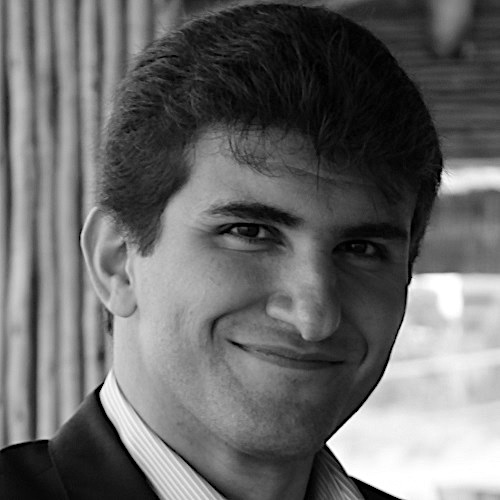
\includegraphics[width=2in]{../media/contributors/MF.jpg} & \textbf{Mohammadali Foroozandeh} \newline \textit{Simon's Ph.D. supervisor} \\

\includegraphics[width=2in]{../media/contributors/TM.png} & \textbf{Thomas Moss} \newline \textit{MChem Student Jan 2020 - June 2020} \newline Helped in extending NMR-EsPy to support 2D data \\
\end{tabular}
\end{center}

\renewcommand{\indexname}{Python Module Index}
\begin{sphinxtheindex}
\let\bigletter\sphinxstyleindexlettergroup
\bigletter{n}
\item\relax\sphinxstyleindexentry{nmrespy.\_cols}\sphinxstyleindexpageref{references/cols:\detokenize{module-nmrespy._cols}}
\item\relax\sphinxstyleindexentry{nmrespy.\_errors}\sphinxstyleindexpageref{references/errors:\detokenize{module-nmrespy._errors}}
\item\relax\sphinxstyleindexentry{nmrespy.\_misc}\sphinxstyleindexpageref{references/misc:\detokenize{module-nmrespy._misc}}
\item\relax\sphinxstyleindexentry{nmrespy.core}\sphinxstyleindexpageref{references/core:\detokenize{module-nmrespy.core}}
\item\relax\sphinxstyleindexentry{nmrespy.freqfilter}\sphinxstyleindexpageref{references/freqfilter:\detokenize{module-nmrespy.freqfilter}}
\item\relax\sphinxstyleindexentry{nmrespy.load}\sphinxstyleindexpageref{references/load:\detokenize{module-nmrespy.load}}
\item\relax\sphinxstyleindexentry{nmrespy.mpm}\sphinxstyleindexpageref{references/mpm:\detokenize{module-nmrespy.mpm}}
\item\relax\sphinxstyleindexentry{nmrespy.nlp.\_funcs}\sphinxstyleindexpageref{references/nlp/_funcs:\detokenize{module-nmrespy.nlp._funcs}}
\item\relax\sphinxstyleindexentry{nmrespy.nlp.nlp}\sphinxstyleindexpageref{references/nlp/nlp:\detokenize{module-nmrespy.nlp.nlp}}
\item\relax\sphinxstyleindexentry{nmrespy.plot}\sphinxstyleindexpageref{references/plot:\detokenize{module-nmrespy.plot}}
\item\relax\sphinxstyleindexentry{nmrespy.sig}\sphinxstyleindexpageref{references/sig:\detokenize{module-nmrespy.sig}}
\item\relax\sphinxstyleindexentry{nmrespy.write}\sphinxstyleindexpageref{references/write:\detokenize{module-nmrespy.write}}
\end{sphinxtheindex}

\renewcommand{\indexname}{Index}
\printindex
\end{document}